% Options for packages loaded elsewhere
\PassOptionsToPackage{unicode}{hyperref}
\PassOptionsToPackage{hyphens}{url}
%
\documentclass[
]{book}
\usepackage{amsmath,amssymb}
\usepackage{iftex}
\ifPDFTeX
  \usepackage[T1]{fontenc}
  \usepackage[utf8]{inputenc}
  \usepackage{textcomp} % provide euro and other symbols
\else % if luatex or xetex
  \usepackage{unicode-math} % this also loads fontspec
  \defaultfontfeatures{Scale=MatchLowercase}
  \defaultfontfeatures[\rmfamily]{Ligatures=TeX,Scale=1}
\fi
\usepackage{lmodern}
\ifPDFTeX\else
  % xetex/luatex font selection
\fi
% Use upquote if available, for straight quotes in verbatim environments
\IfFileExists{upquote.sty}{\usepackage{upquote}}{}
\IfFileExists{microtype.sty}{% use microtype if available
  \usepackage[]{microtype}
  \UseMicrotypeSet[protrusion]{basicmath} % disable protrusion for tt fonts
}{}
\makeatletter
\@ifundefined{KOMAClassName}{% if non-KOMA class
  \IfFileExists{parskip.sty}{%
    \usepackage{parskip}
  }{% else
    \setlength{\parindent}{0pt}
    \setlength{\parskip}{6pt plus 2pt minus 1pt}}
}{% if KOMA class
  \KOMAoptions{parskip=half}}
\makeatother
\usepackage{xcolor}
\usepackage{listings}
\newcommand{\passthrough}[1]{#1}
\lstset{defaultdialect=[5.3]Lua}
\lstset{defaultdialect=[x86masm]Assembler}
\usepackage{longtable,booktabs,array}
\usepackage{calc} % for calculating minipage widths
% Correct order of tables after \paragraph or \subparagraph
\usepackage{etoolbox}
\makeatletter
\patchcmd\longtable{\par}{\if@noskipsec\mbox{}\fi\par}{}{}
\makeatother
% Allow footnotes in longtable head/foot
\IfFileExists{footnotehyper.sty}{\usepackage{footnotehyper}}{\usepackage{footnote}}
\makesavenoteenv{longtable}
\usepackage{graphicx}
\makeatletter
\newsavebox\pandoc@box
\newcommand*\pandocbounded[1]{% scales image to fit in text height/width
  \sbox\pandoc@box{#1}%
  \Gscale@div\@tempa{\textheight}{\dimexpr\ht\pandoc@box+\dp\pandoc@box\relax}%
  \Gscale@div\@tempb{\linewidth}{\wd\pandoc@box}%
  \ifdim\@tempb\p@<\@tempa\p@\let\@tempa\@tempb\fi% select the smaller of both
  \ifdim\@tempa\p@<\p@\scalebox{\@tempa}{\usebox\pandoc@box}%
  \else\usebox{\pandoc@box}%
  \fi%
}
% Set default figure placement to htbp
\def\fps@figure{htbp}
\makeatother
\setlength{\emergencystretch}{3em} % prevent overfull lines
\providecommand{\tightlist}{%
  \setlength{\itemsep}{0pt}\setlength{\parskip}{0pt}}
\setcounter{secnumdepth}{5}
\usepackage{booktabs}

\lstset{
  breaklines=true
  basicstyle=\ttfamily
}
\usepackage{booktabs}
\usepackage{longtable}
\usepackage{array}
\usepackage{multirow}
\usepackage{wrapfig}
\usepackage{float}
\usepackage{colortbl}
\usepackage{pdflscape}
\usepackage{tabu}
\usepackage{threeparttable}
\usepackage{threeparttablex}
\usepackage[normalem]{ulem}
\usepackage{makecell}
\usepackage{xcolor}
\usepackage[]{natbib}
\bibliographystyle{apalike}
\usepackage{bookmark}
\IfFileExists{xurl.sty}{\usepackage{xurl}}{} % add URL line breaks if available
\urlstyle{same}
\hypersetup{
  pdftitle={Uncovering Data Science with R},
  hidelinks,
  pdfcreator={LaTeX via pandoc}}

\title{Uncovering Data Science with R}
\author{}
\date{\vspace{-2.5em}2025-02-06}

\usepackage{amsthm}
\newtheorem{theorem}{Theorem}[chapter]
\newtheorem{lemma}{Lemma}[chapter]
\newtheorem{corollary}{Corollary}[chapter]
\newtheorem{proposition}{Proposition}[chapter]
\newtheorem{conjecture}{Conjecture}[chapter]
\theoremstyle{definition}
\newtheorem{definition}{Definition}[chapter]
\theoremstyle{definition}
\newtheorem{example}{Example}[chapter]
\theoremstyle{definition}
\newtheorem{exercise}{Exercise}[chapter]
\theoremstyle{definition}
\newtheorem{hypothesis}{Hypothesis}[chapter]
\theoremstyle{remark}
\newtheorem*{remark}{Remark}
\newtheorem*{solution}{Solution}
\begin{document}
\maketitle

{
\setcounter{tocdepth}{1}
\tableofcontents
}
\chapter*{Preface}\label{preface}
\addcontentsline{toc}{chapter}{Preface}

\textbf{Data science is transforming the way we solve problems, make decisions, and uncover insights from data.} Whether you're a beginner or an experienced professional, \emph{Uncovering Data Science with R} provides an intuitive and practical introduction to this exciting field---no prior analytics or programming experience required.

This book is a work in progress, and we welcome feedback from readers. If you have any comments, suggestions, or corrections, please feel free to contact us at \href{mailto:a.mohammadi@uva.nl}{Contact Us}.

\section*{Why This Book?}\label{why-this-book}
\addcontentsline{toc}{section}{Why This Book?}

Data science is a rapidly evolving field that leverages computational tools and techniques to transform raw data into actionable insights. In this book, we introduce the fundamental skills needed to work with \textbf{R}, a powerful and freely available statistical programming language widely used for data analysis, visualization, and machine learning.

Unlike many other books on data science, our focus is on accessibility. We aim to provide an intuitive and practical introduction, making \textbf{R} and data science concepts understandable for those with little or no technical background. Our hands-on approach ensures that you will not only learn theoretical concepts but also gain experience applying them to real-world datasets.

Compared to commercial software like SAS or SPSS, \textbf{R} provides a free, open-source, and highly extensible platform for statistical computing and machine learning. Its rich ecosystem of packages makes it an excellent alternative to proprietary data mining tools.

Inspired by the Free and Open Source Software (FOSS) movement, the content of this book is open and transparent, ensuring reproducibility. The code, datasets, and materials are hosted on \href{https://cran.r-project.org/web/packages/liver/index.html}{CRAN} and are accessible via the \textbf{liver} package (\url{https://CRAN.R-project.org/package=liver}), allowing readers to engage with the book interactively.

\section*{Who Should Read This Book?}\label{who-should-read-this-book}
\addcontentsline{toc}{section}{Who Should Read This Book?}

This book is for anyone interested in learning about data science, particularly those new to the field. It is designed for:

\begin{itemize}
\tightlist
\item
  Business professionals who want to leverage data for decision-making,\\
\item
  Students and researchers looking to apply data analysis in their work,\\
\item
  Beginners with no prior programming experience,\\
\item
  Anyone interested in data science and machine learning using \textbf{R}.
\end{itemize}

\section*{What You Will Learn}\label{what-you-will-learn}
\addcontentsline{toc}{section}{What You Will Learn}

The primary goal of this book is to introduce data science concepts using \textbf{R} as a tool for data analysis and machine learning. \textbf{R} is an open-source language and environment for statistical computing and graphics, offering a vast collection of packages for data mining, visualization, and modeling.

Through hands-on examples and real-world datasets, you will learn:

\begin{itemize}
\tightlist
\item
  The basics of \textbf{R} and how to set up your environment,\\
\item
  The core principles of data science and the Data Science Methodology,\\
\item
  How to clean, transform, and explore data,\\
\item
  The fundamentals of statistical analysis, machine learning, and data visualization,\\
\item
  How to build and evaluate machine learning models, including classification, regression, clustering, and neural networks,\\
\item
  How to apply these techniques to real-world datasets.
\end{itemize}

\section*{The Data Science Process}\label{the-data-science-process}
\addcontentsline{toc}{section}{The Data Science Process}

Data science follows an iterative and structured methodology for analyzing and extracting insights from data. This book follows this framework:

\begin{enumerate}
\def\labelenumi{\arabic{enumi}.}
\tightlist
\item
  \textbf{Problem Understanding} -- Defining the objective and understanding the data.\\
\item
  \textbf{Data Preparation} -- Preparing raw data for analysis.\\
\item
  \textbf{Exploratory Data Analysis (EDA)} -- Identifying patterns and relationships in data.\\
\item
  \textbf{Preparing Data for Modeling} -- Transforming data for machine learning models.\\
\item
  \textbf{Modeling} -- Building predictive models using machine learning algorithms.\\
\item
  \textbf{Evaluation} -- Assessing model performance using various metrics.\\
\item
  \textbf{Deployment} -- Applying the trained model to real-world scenarios.
\end{enumerate}

By the end of this book, you will have a solid understanding of these phases and be able to apply them effectively.

\section*{How This Book Is Structured}\label{how-this-book-is-structured}
\addcontentsline{toc}{section}{How This Book Is Structured}

This book is structured as a \textbf{hands-on guide}, designed to take you from beginner to practitioner in \textbf{R} and data science. The chapters follow a logical progression, starting with foundational concepts and gradually introducing more advanced techniques.

We use \textbf{real-world datasets} (see Table \ref{tab:data-table}) throughout the book to illustrate key concepts. These datasets are available in the \textbf{liver} package and can be accessed easily. Below is a brief overview of the book's chapters:

\begin{itemize}
\tightlist
\item
  \textbf{Chapter \ref{chapter-into-R}} -- Introduction to \textbf{R}, including installation and basic operations.\\
\item
  \textbf{Chapter \ref{chapter-intro-DS}} -- Introduction to Data Science and its methodology.\\
\item
  \textbf{Chapter \ref{chapter-data-prep}} -- Data preparation techniques.\\
\item
  \textbf{Chapter \ref{chapter-EDA}} -- Exploratory Data Analysis (EDA) using visualization and summary statistics.\\
\item
  \textbf{Chapter \ref{chapter-statistics}} -- Basics of statistical analysis, including descriptive statistics and hypothesis testing.\\
\item
  \textbf{Chapter \ref{chapter-modeling}} -- Overview of machine learning models.\\
\item
  \textbf{Chapter \ref{chapter-knn}} -- k-Nearest Neighbors (k-NN) algorithm.\\
\item
  \textbf{Chapter \ref{chapter-evaluation}} -- Model evaluation metrics and techniques.\\
\item
  \textbf{Chapter \ref{chapter-bayes}} -- Naïve Bayes classifier for probabilistic modeling.\\
\item
  \textbf{Chapter \ref{chapter-regression}} -- Linear regression for predictive modeling.\\
\item
  \textbf{Chapter \ref{chapter-tree}} -- Decision trees and Random Forests.\\
\item
  \textbf{Chapter \ref{chapter-nn}} -- Neural networks and deep learning basics.\\
\item
  \textbf{Chapter \ref{chapter-cluster}} -- Clustering techniques, including k-means.
\end{itemize}

At the end of each chapter, you will find \textbf{practical exercises and labs} to reinforce your learning. These exercises use real-world datasets and provide step-by-step guidance to ensure hands-on experience.

\section*{How to Use This Book}\label{how-to-use-this-book}
\addcontentsline{toc}{section}{How to Use This Book}

This book is designed for \textbf{both self-study and classroom use}. You can read it cover to cover or jump to the chapters that interest you most. Each chapter builds on the previous ones, so beginners are encouraged to follow the sequence for a smooth learning experience.

To get the most out of this book:

\begin{itemize}
\tightlist
\item
  \textbf{Run the code examples} -- All code snippets are designed to be executed interactively in \textbf{R}.\\
\item
  \textbf{Complete the exercises} -- Practical exercises reinforce key concepts and improve problem-solving skills.\\
\item
  \textbf{Modify and experiment} -- Try changing the code to explore different scenarios.\\
\item
  \textbf{Use it as a reference} -- Once you're familiar with the basics, use this book as a guide for working with real-world data.
\end{itemize}

This book has also been used in \textbf{data science courses} at the University of Amsterdam. It can serve as a textbook for similar courses or as a supplementary resource for more advanced analytics training.

\section*{Datasets Used in This Book}\label{datasets-used-in-this-book}
\addcontentsline{toc}{section}{Datasets Used in This Book}

Table \ref{tab:data-table} lists the datasets used in this book. These real-world datasets are used to illustrate key concepts and are available in the \textbf{liver} package, which can be downloaded from CRAN.

\begin{table}
\centering
\caption{\label{tab:data-table}List of datasets used for case studies in different chapters. Available in the R package liver.}
\centering
\begin{tabular}[t]{>{}l>{\raggedright\arraybackslash}p{20em}l}
\toprule
Name & Description & Chapter\\
\midrule
\textcolor{black}{\textbf{churn}} & Customer churn dataset. & Chapters 4, 6, 8, 10\\
\textcolor{black}{\textbf{bank}} & Direct marketing data from a Portuguese bank. & Chapter 7, 12\\
\textcolor{black}{\textbf{adult}} & US Census data for income prediction. & Chapter 11\\
\textcolor{black}{\textbf{risk}} & Credit risk dataset. & Chapter 9\\
\textcolor{black}{\textbf{marketing}} & Marketing campaign performance data. & Chapter 10\\
\addlinespace
\textcolor{black}{\textbf{house}} & House price prediction dataset. & Chapter 10\\
\textcolor{black}{\textbf{diamonds}} & Diamond pricing dataset. & Chapter 3\\
\textcolor{black}{\textbf{cereal}} & Nutritional information for 77 breakfast cereals. & Chapter 13\\
\bottomrule
\end{tabular}
\end{table}

\section*{Prerequisites}\label{prerequisites}
\addcontentsline{toc}{section}{Prerequisites}

No prior programming experience is required, but a basic understanding of numbers and logic will be helpful. To run the code in this book, you need to install \textbf{R}, \textbf{RStudio}, and several \textbf{R} packages.

\chapter{The Basics for R}\label{chapter-into-R}

Before you can analyze data, you need a way to communicate with your computer. That's where programming languages like R and Python come in. Many data science teams use a mix of languages, but R is a great starting point because it is designed specifically for data analysis and statistical computing.

R offers a rich ecosystem of libraries and tools tailored for data science. It has a simple yet expressive syntax, making it easy to explore and manipulate data. Unlike general-purpose programming languages, R was built for statistical analysis, allowing data scientists to perform everything from basic calculations to advanced machine learning with just a few lines of code.

Beyond its capabilities, R is:

\begin{itemize}
\tightlist
\item
  Free \& Open Source -- Available to everyone, with a vibrant community of contributors.\\
\item
  Cross-Platform -- Runs on Windows, macOS, and Linux.\\
\item
  Flexible \& Powerful -- Supports interactive data exploration, visualization, and machine learning.
\end{itemize}

While R is the language, RStudio is the tool that makes working with R easier. RStudio is an integrated development environment (IDE) that provides:

\begin{itemize}
\tightlist
\item
  A console for running R commands,\\
\item
  A script editor with syntax highlighting and auto-completion,\\
\item
  Built-in tools for data visualization, debugging, and package management.
\end{itemize}

In this chapter, you will learn the fundamental skills needed to work with R, from installation to running your first commands. Let's begin! 🚀

\section{How to Install R}\label{how-to-install-r}

To get started with R, you first need to install it on your computer. Follow these steps:

\begin{enumerate}
\def\labelenumi{\arabic{enumi}.}
\tightlist
\item
  Go to the \href{https://cran.r-project.org}{CRAN website} -- The Comprehensive R Archive Network.\\
\item
  Select your operating system -- Click the link for Windows, macOS, or Linux.\\
\item
  Download and install R -- Follow the on-screen instructions to complete the installation.
\end{enumerate}

\subsection*{Keeping R Up to Date}\label{keeping-r-up-to-date}
\addcontentsline{toc}{subsection}{Keeping R Up to Date}

R receives a major update once a year, along with 2-3 minor updates annually. While updating R---especially major versions---requires reinstalling your packages, staying up to date ensures you:

✅ Access the latest features and improvements,\\
✅ Maintain compatibility with new packages,\\
✅ Benefit from security patches and performance enhancements.

Keeping R updated might feel like a hassle, but postponing updates can make the process more cumbersome later. It's best to update regularly to ensure smooth performance and compatibility.

\section{How to Install RStudio}\label{how-to-install-rstudio}

RStudio is an open-source integrated development environment (IDE) that makes working with R easier, more interactive, and more efficient. It provides a user-friendly interface, an advanced script editor, and various tools for plotting, debugging, and workspace management---all of which significantly enhance the R programming experience.

\subsection*{Installing RStudio}\label{installing-rstudio}
\addcontentsline{toc}{subsection}{Installing RStudio}

Follow these steps to install RStudio:

\begin{enumerate}
\def\labelenumi{\arabic{enumi}.}
\tightlist
\item
  Go to the \href{http://www.rstudio.com/download}{RStudio website}.\\
\item
  Download the latest version of RStudio Desktop (the free, open-source edition).\\
\item
  Run the installer and follow the on-screen instructions.\\
\item
  Launch RStudio, and you're ready to start coding in R!
\end{enumerate}

RStudio is updated several times a year, and it will notify you when a new version is available. Keeping RStudio up to date is recommended to take advantage of new features and performance improvements.

\subsection*{Exploring the RStudio Interface}\label{exploring-the-rstudio-interface}
\addcontentsline{toc}{subsection}{Exploring the RStudio Interface}

When you open RStudio, you will see a window similar to Figure \ref{fig:RStudio-window-1}.

\begin{figure}

{\centering 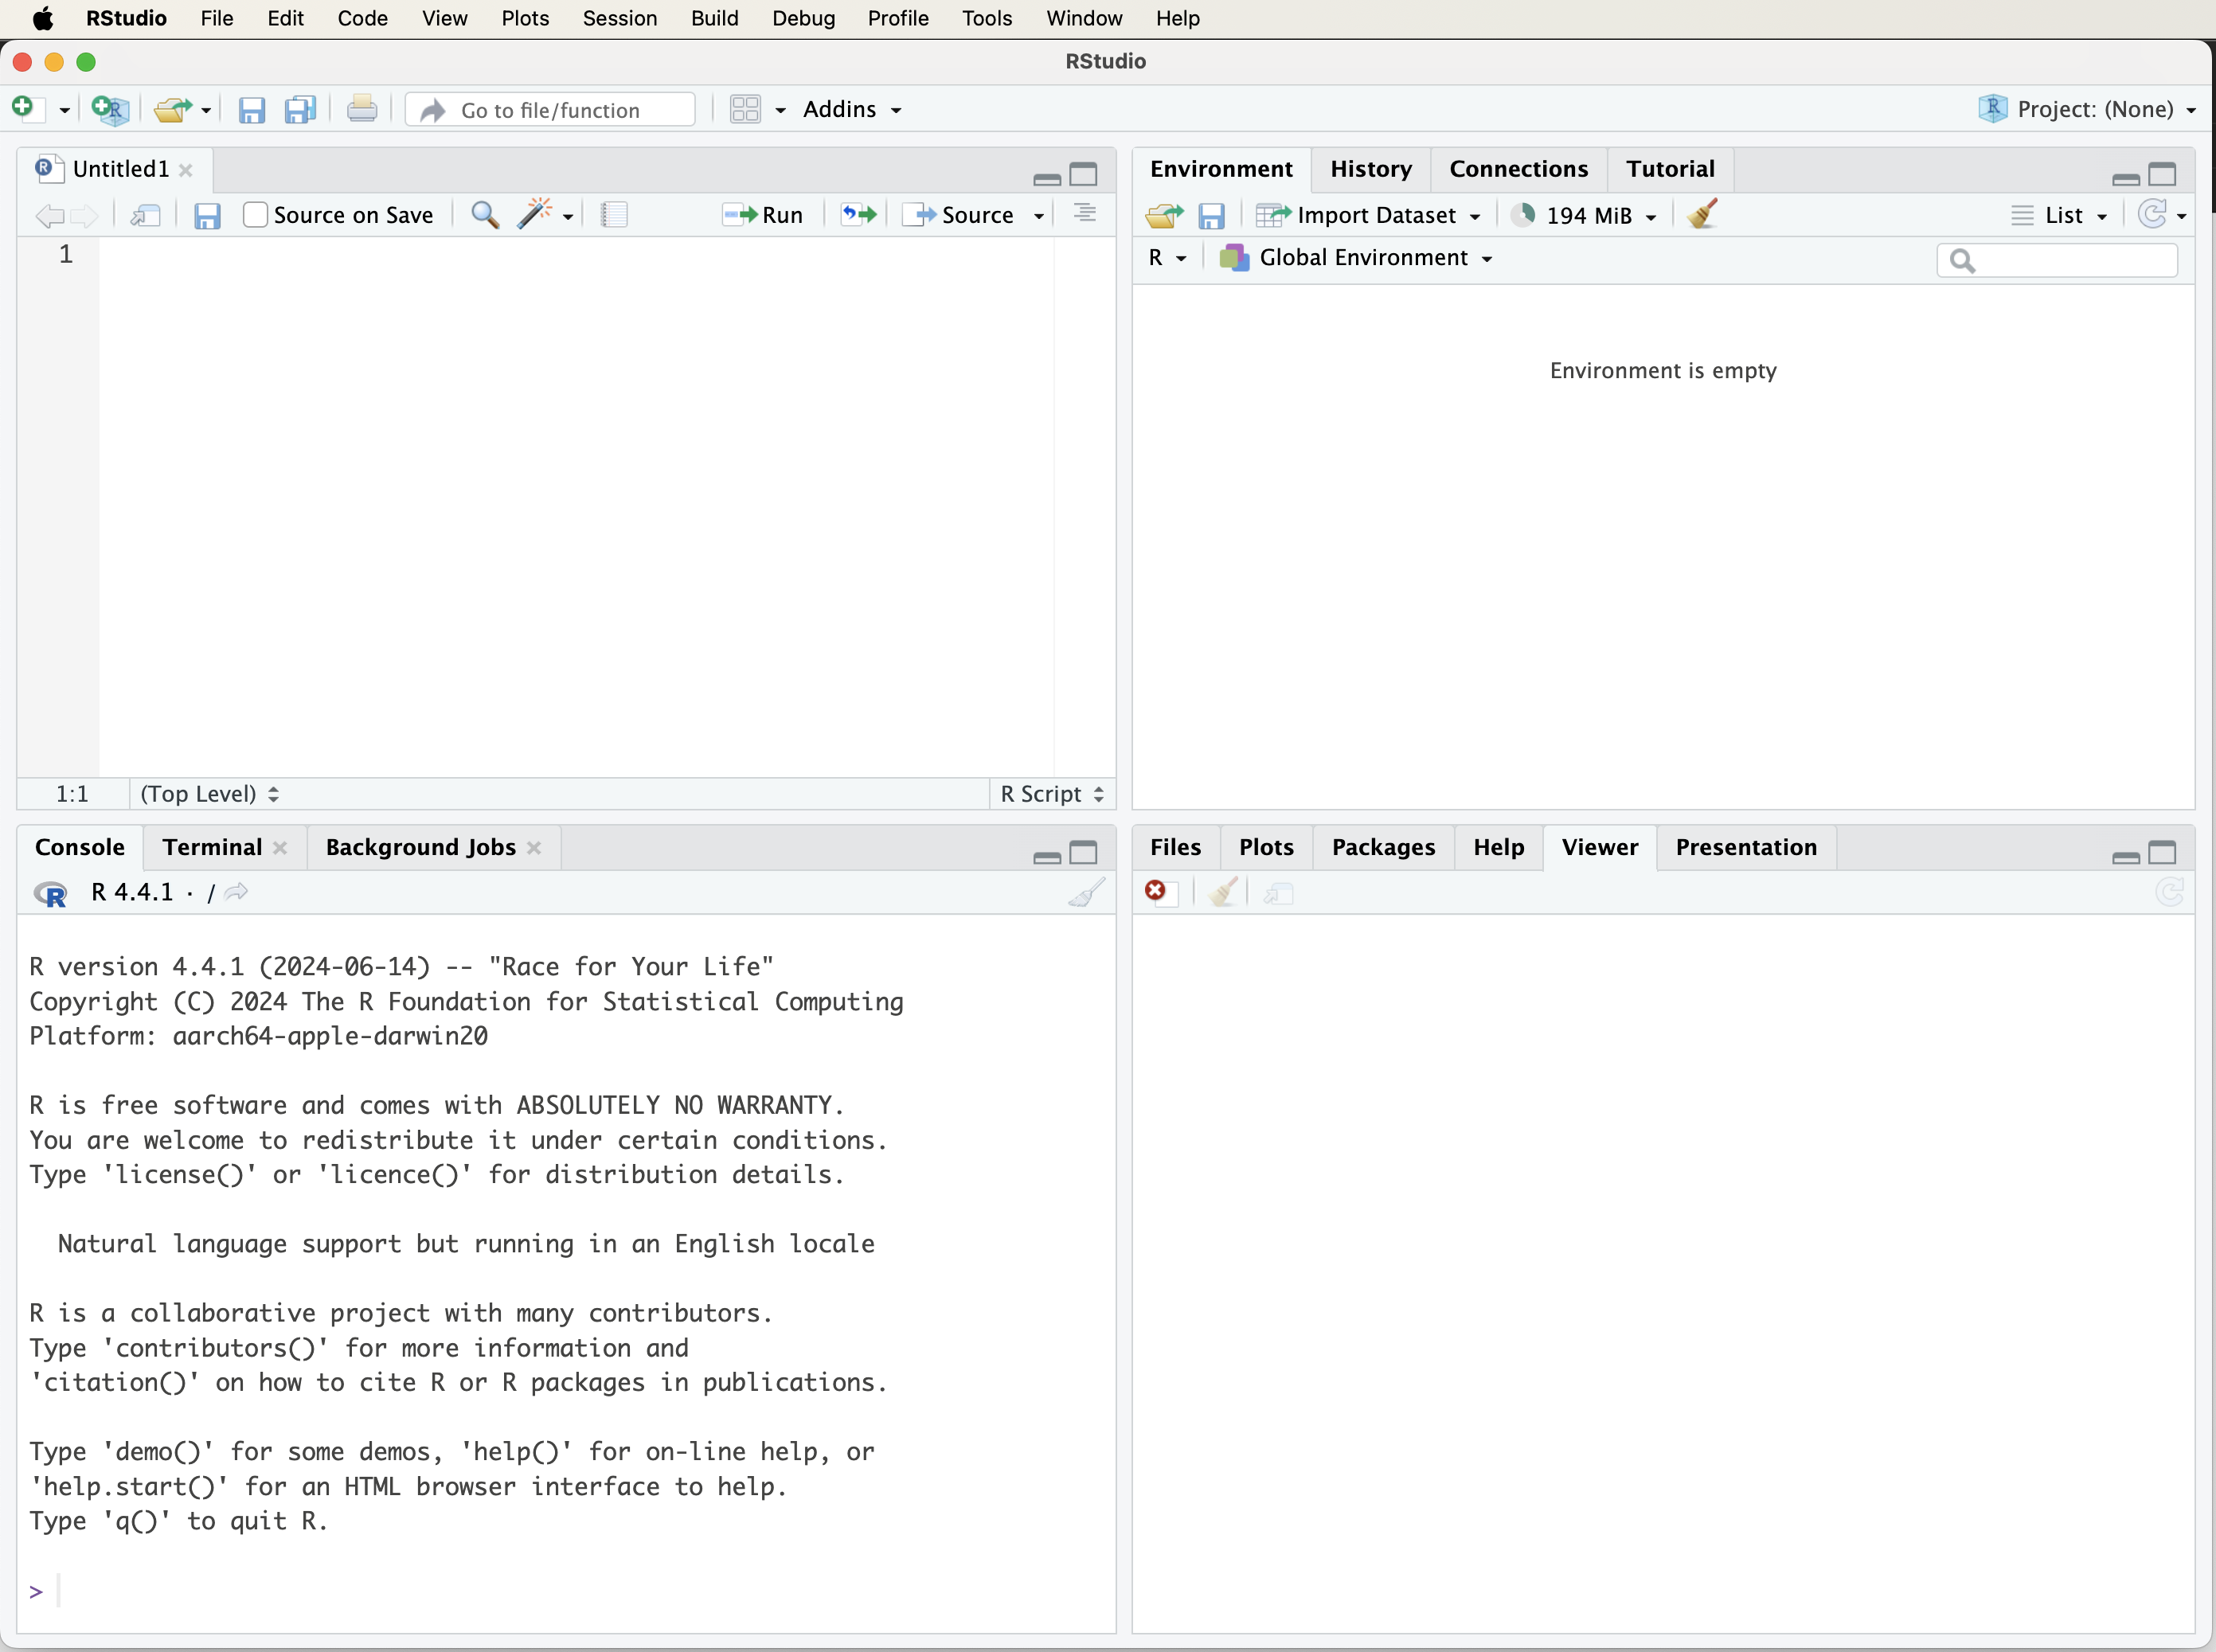
\includegraphics[width=0.7\linewidth]{images/RStudio-window-1} 

}

\caption{The RStudio window when you first launch the program.}\label{fig:RStudio-window-1}
\end{figure}

If you see only three panels, add a fourth by selecting \emph{File \textgreater{} New File \textgreater{} R Script}. This opens a script editor where you can write and save R code. Here's a quick overview of RStudio's panels:

\begin{itemize}
\tightlist
\item
  Top-left: Script Editor -- Write and save your R code.\\
\item
  Bottom-left: Console -- Run R commands and see output.\\
\item
  Top-right: Environment \& History -- View variables, datasets, and past commands.\\
\item
  Bottom-right: Plots, Help, \& Files -- Display graphs, access documentation, and manage files.
\end{itemize}

For now, just know that you can type R code into the console and press Enter to run it. As you progress through the book, you'll become more familiar with RStudio's features and learn how to efficiently write, run, and debug R code.

\subsection*{Customizing RStudio}\label{customizing-rstudio}
\addcontentsline{toc}{subsection}{Customizing RStudio}

RStudio is highly customizable, allowing you to tailor it to your workflow. To adjust settings, go to:

\begin{itemize}
\tightlist
\item
  Tools \textgreater{} Global Options -- Access general settings.\\
\item
  Appearance \textgreater{} Editor Theme -- Change the editor's theme (e.g., ``Tomorrow Night 80'' for a dark mode).\\
\item
  Font \& Layout Settings -- Modify font size, panel positions, and other interface options.\\
  A comfortable coding environment enhances productivity---so feel free to explore and tweak the settings to suit your preferences!
\end{itemize}

\section{How to Learn R}\label{how-to-learn-r}

Learning R is an exciting and rewarding journey that opens doors to data science, statistics, and machine learning. Fortunately, there are numerous resources---books, online courses, tutorials, and forums---that can help you get started and advance your skills.

\subsection*{1. Video Tutorials}\label{video-tutorials}
\addcontentsline{toc}{subsection}{1. Video Tutorials}

If you prefer learning by watching, YouTube offers a wealth of R tutorials, ranging from beginner to advanced levels:

\begin{itemize}
\tightlist
\item
  \href{https://www.youtube.com/channel/UCJ7w9dVjTOJi8Z7j0y9v6Qw}{R Programming} -- Covers R basics and data science concepts.\\
\item
  \href{https://www.youtube.com/user/dataschool}{Data School} -- Focuses on data analysis, machine learning, and practical R applications.
\end{itemize}

\subsection*{2. Books}\label{books}
\addcontentsline{toc}{subsection}{2. Books}

Books are a great way to build a deep understanding of R. Here are some top recommendations:

\begin{itemize}
\tightlist
\item
  For Absolute Beginners: \href{https://rstudio-education.github.io/hopr/}{\emph{Hands-On Programming with R}} by Garrett Grolemund\citep{grolemund2014hands} -- A practical introduction for those new to programming.\\
\item
  For Data Science with R: \href{https://r4ds.had.co.nz}{\emph{R for Data Science}} by Hadley Wickham and Garrett Grolemund \citep{wickham2017r} -- Covers data visualization, wrangling, and modeling.\\
\item
  For Machine Learning: \href{https://www.packtpub.com/product/machine-learning-with-r/9781782162148}{\emph{Machine Learning with R}} by Brett Lantz\citep{lantz2013machine} -- A comprehensive guide to machine learning techniques using R.
\end{itemize}

\subsection*{3. Online Courses}\label{online-courses}
\addcontentsline{toc}{subsection}{3. Online Courses}

If you prefer structured learning with hands-on exercises, online courses offer interactive experiences:

\begin{itemize}
\tightlist
\item
  \href{https://www.datacamp.com}{DataCamp} -- Features beginner-friendly courses like \href{https://learn.datacamp.com/courses/free-introduction-to-r}{\emph{Introduction to R}}.\\
\item
  \href{https://www.coursera.org}{Coursera} -- Offers courses such as \href{https://www.coursera.org/learn/r-programming}{\emph{R Programming}} and the \href{https://www.coursera.org/specializations/jhu-data-science}{\emph{Data Science Specialization}}.
\end{itemize}

\subsection*{4. R Communities \& Forums}\label{r-communities-forums}
\addcontentsline{toc}{subsection}{4. R Communities \& Forums}

Engaging with online communities is a great way to learn from others, ask questions, and get support:

\begin{itemize}
\tightlist
\item
  \href{https://stackoverflow.com/questions/tagged/r}{Stack Overflow} -- Find answers to R-related coding questions.\\
\item
  \href{https://community.rstudio.com/}{RStudio Community} -- Connect with other R users and participate in discussions.
\end{itemize}

\subsection*{5. Practice Regularly}\label{practice-regularly}
\addcontentsline{toc}{subsection}{5. Practice Regularly}

The best way to learn R is through consistent practice. Start with simple exercises, explore real-world datasets, and experiment with R code. By combining structured learning with hands-on experience, you'll quickly develop confidence and proficiency in R.

🚀 Start today! Choose one of the resources above and begin your R learning journey.

\section{Getting Help and Learning More}\label{getting-help-and-learning-more}

As you begin your journey with R, you'll likely encounter challenges and questions along the way. Fortunately, there are many resources available to help you troubleshoot problems, deepen your understanding, and continue learning. Whether you're stuck on an error message, exploring a new function, or looking for best practices, a combination of built-in documentation, online communities, and external learning materials can guide you.

R comes with extensive built-in documentation that provides details on functions, packages, and programming techniques. To quickly look up a function, type \passthrough{\lstinline!?!} followed by the function name in the R console. This will bring up official documentation, including usage examples, argument details, and additional references. You can also use \passthrough{\lstinline!help()!} or \passthrough{\lstinline!example()!} to get more context on how a function works.

Beyond R's internal help system, the R community is an invaluable resource. If you have a question, chances are someone has already asked (and answered) it. Platforms like Stack Overflow, RStudio Community, and the R-help mailing list contain thousands of discussions on common and advanced topics in R programming, data science, and machine learning. Searching these forums can often lead you to quick and reliable solutions. If you don't find an existing answer, posting your question with a clear explanation and a reproducible example will increase your chances of getting helpful responses.

A simple Google search is often the fastest way to troubleshoot issues. Searching for an error message or function name will usually direct you to blog posts, documentation, or forum discussions with relevant explanations. Additionally, AI tools like ChatGPT can assist with R programming questions, debugging, and conceptual explanations. While AI-generated solutions aren't always perfect, they can provide useful insights, suggest alternative approaches, and help clarify difficult concepts.

Ultimately, the best way to master R is through hands-on experience. Don't be afraid to experiment---write code, test different functions, and explore new datasets. Mistakes are a natural part of learning, and each one helps reinforce your understanding. The more you practice, the more confident and proficient you'll become in R. Keep coding, keep exploring, and enjoy the journey!

\section{Data Science with R}\label{data-science-with-r}

R provides a strong foundation for data science, but its real power comes from its extensive ecosystem of packages---collections of functions, datasets, and documentation that extend R's capabilities. While the base version of R includes many essential tools, it does not come preloaded with all the statistical and machine learning algorithms you may need. Instead, these algorithms are developed and shared by a large community of researchers and practitioners as free and open-source R packages.

A package is a modular, reusable library that enhances R's functionality. Packages include well-documented functions, usage instructions, and often sample datasets for testing and learning. In this book, we frequently use the \textbf{liver} package, which was developed specifically to accompany this book. It contains datasets and functions designed to illustrate key data science concepts and techniques. Additionally, for each machine learning algorithm covered in this book, we introduce and use the appropriate R packages that implement those methods.

For those interested in exploring further, the Comprehensive R Archive Network (CRAN) hosts thousands of packages for statistical computing, data visualization, and machine learning. The full list of available packages can be browsed on the \href{https://CRAN.R-project.org}{CRAN website}, providing access to tools tailored to various domains in data science and beyond.

\section{How to Install R Packages}\label{install-packages}

There are two ways to install R packages. The first method is through RStudio's graphical interface. Click on the ``Tools'' tab and select ``Install Packages\ldots{}''. In the dialog box that appears, enter the name of the package(s) you wish to install in the ``Packages'' field and click the ``Install'' button. Make sure to check the ``Install dependencies'' option to ensure that all necessary supporting packages are installed as well. See Figure \ref{fig:install-packages} for a visual guide.

\begin{figure}

{\centering 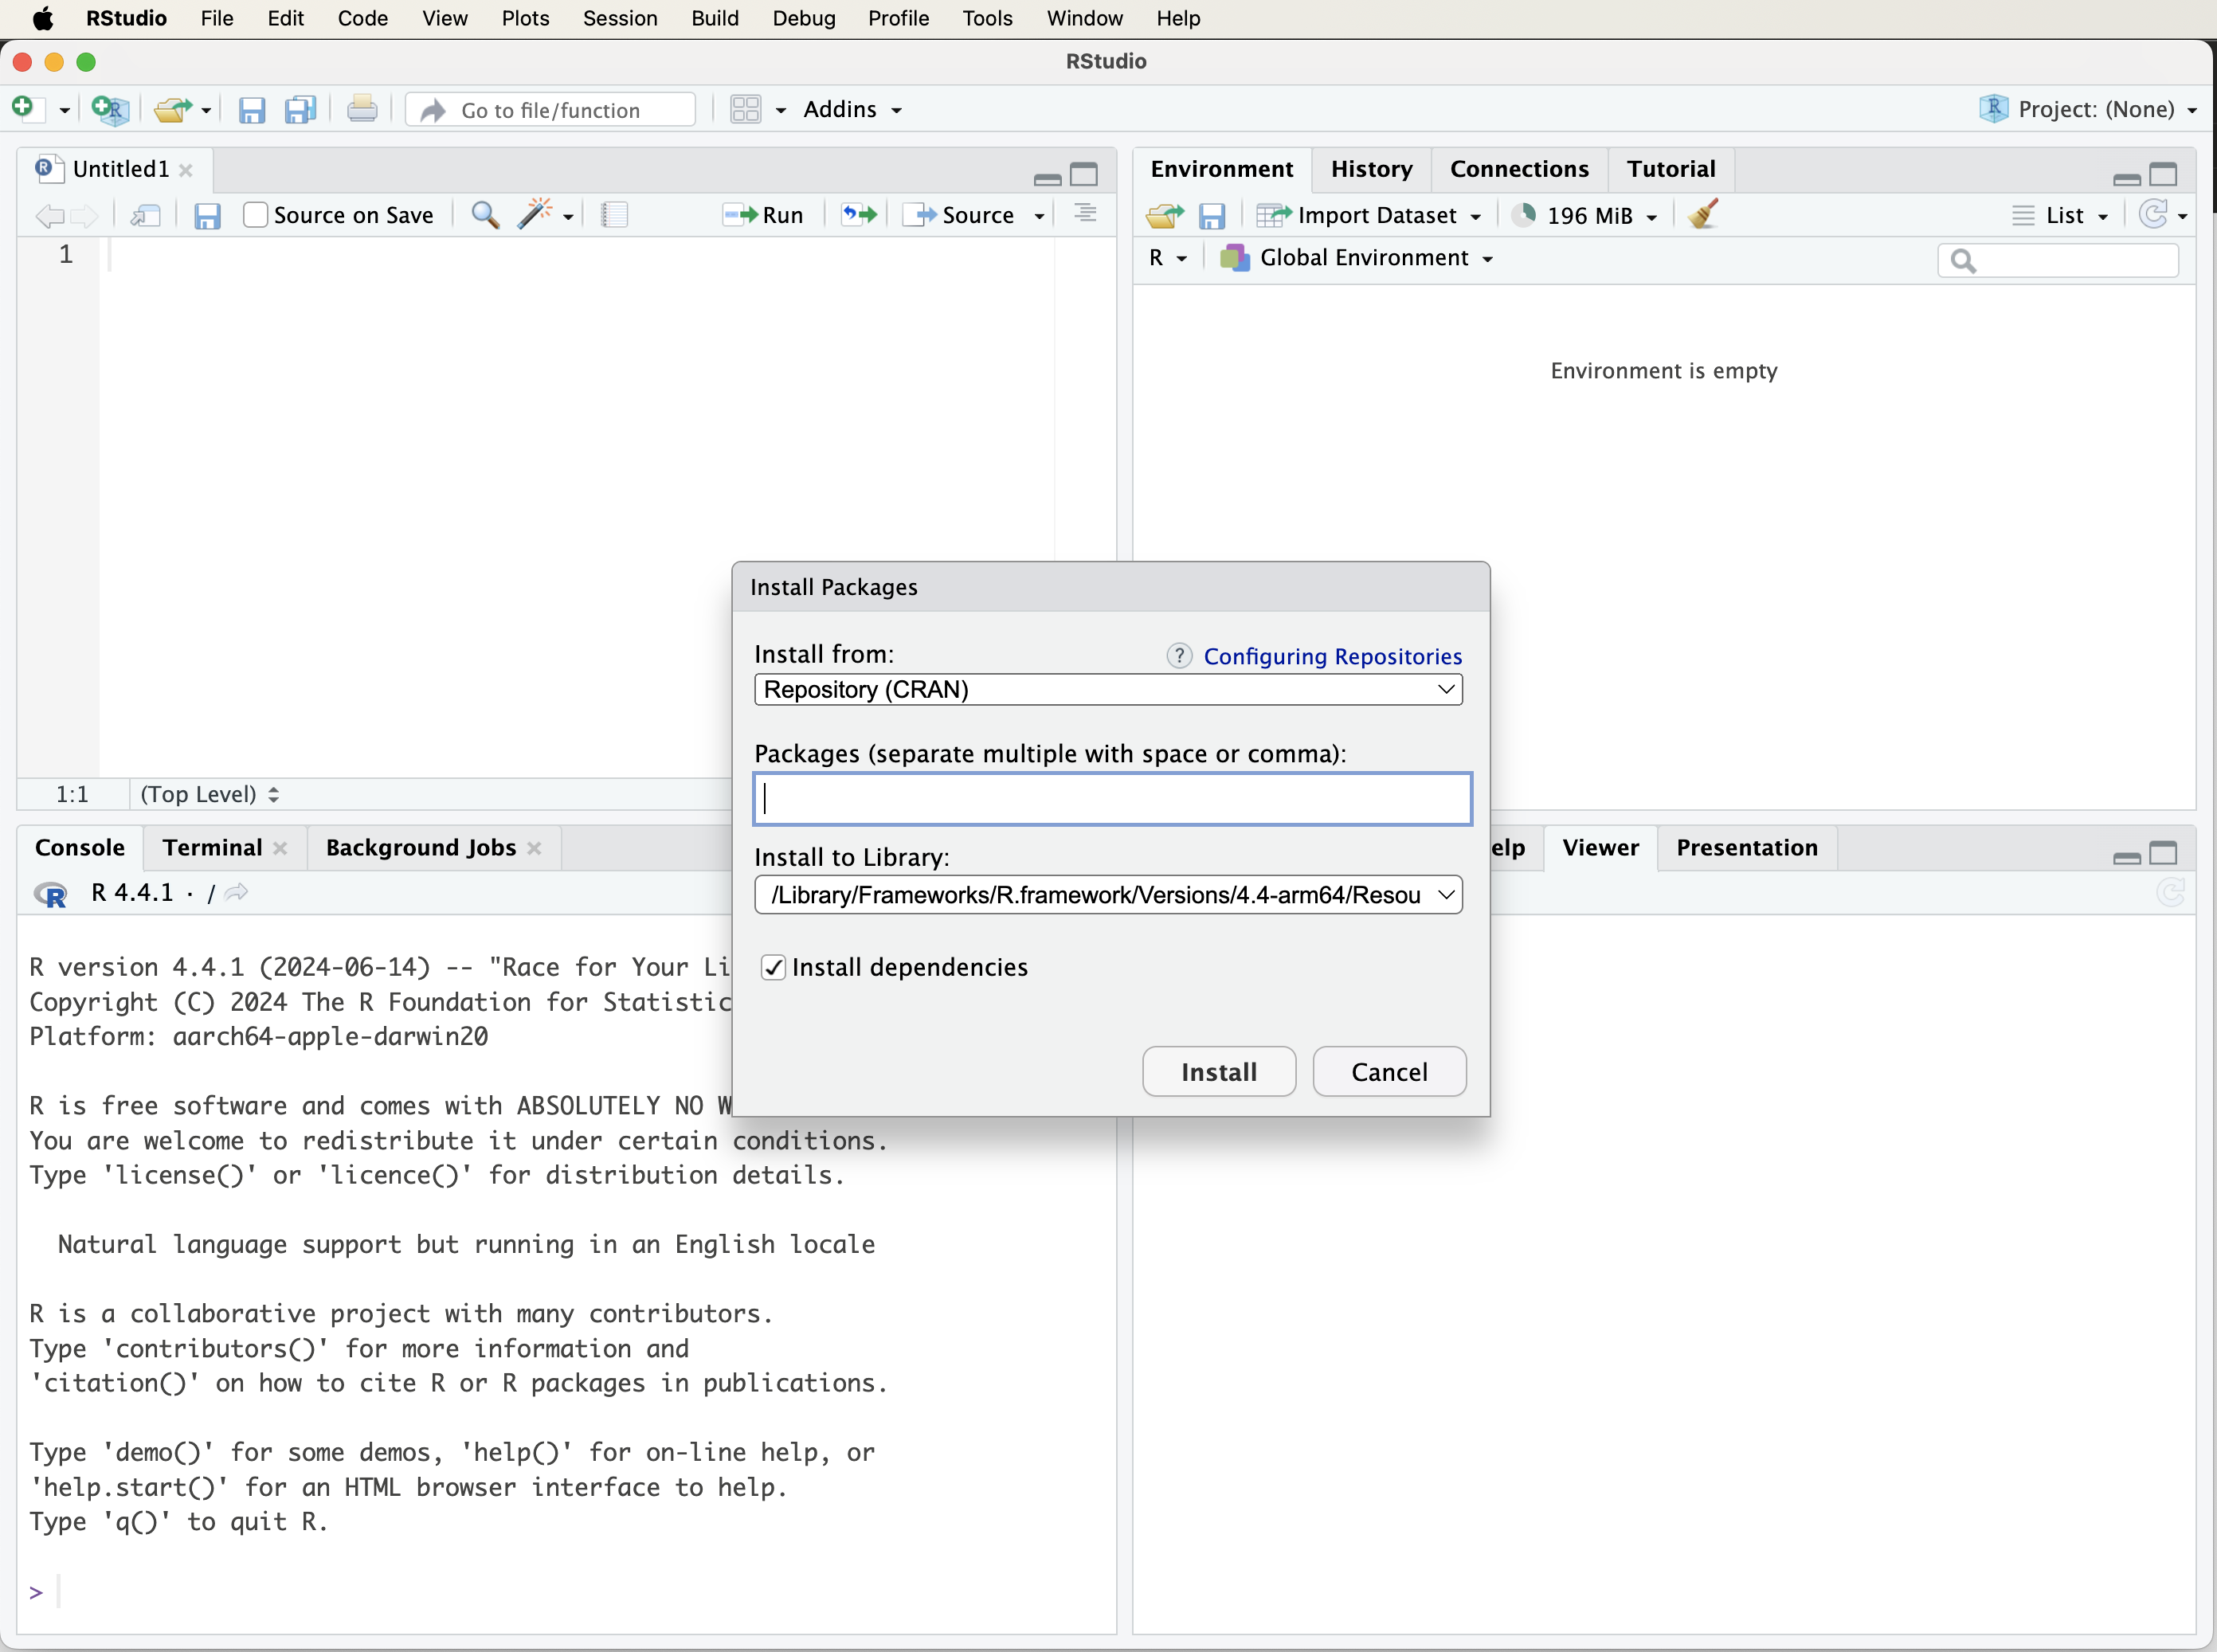
\includegraphics[width=0.7\linewidth]{images/RStudio-window-install} 

}

\caption{A visual guide to installing R packages using the 'Tools' tab in RStudio.}\label{fig:install-packages}
\end{figure}

The second method is to install packages directly using the \passthrough{\lstinline!install.packages()!} function. For example, to install the \textbf{liver} package, which provides datasets and functions used throughout this book, enter the following command in the R console:

\begin{lstlisting}[language=R]
install.packages("liver")
\end{lstlisting}

Press ``Enter'' to execute the command. R will connect to \href{https://cran.r-project.org}{CRAN} and download the package in the correct format for your operating system. If you encounter any issues during installation, ensure you are connected to the internet and that your proxy or firewall is not blocking access to CRAN. The first time you install a package, R may ask you to select a CRAN mirror. Choose one that is geographically close to you for faster downloads.

The \passthrough{\lstinline!install.packages()!} function also allows for customization, such as installing a package from a local file or a specific repository. To learn more, type the following command in the R console:

\begin{lstlisting}[language=R]
?install.packages()
\end{lstlisting}

Packages only need to be installed once. After installation, they must be loaded into each new R session using the \passthrough{\lstinline!library()!} function. We will cover how to load packages in the next section.

\section{How to Load R Packages}\label{how-to-load-r-packages}

To optimize memory usage, R does not automatically load all installed packages. Instead, you must explicitly load the necessary packages in each new R session. This ensures that only relevant functions and datasets are available, minimizing resource consumption.\\
To load a package, use the \passthrough{\lstinline!library()!} or \passthrough{\lstinline!require()!} function. These functions locate the package on your system and make its functions, datasets, and documentation accessible. For example, to load the \textbf{liver} package, enter the following command in the R console:

\begin{lstlisting}[language=R]
library(liver)
\end{lstlisting}

Press \emph{Enter} to execute the command. If an error message appears stating that the package is not found (e.g., \passthrough{\lstinline!"there is no package called 'liver'"!}), it indicates that the package has not been installed. In such cases, refer to the previous section on installing packages.

Beyond \textbf{liver}, this book utilizes several other R packages, which will be introduced progressively throughout the chapters as needed. However, some R packages contain functions with identical names. For instance, both the \textbf{liver* and }dplyr** packages include a \passthrough{\lstinline!select()!} function. When multiple packages are loaded, R defaults to using the function from the most recently loaded package.

To explicitly specify which package a function should be sourced from, use the \passthrough{\lstinline!::!} operator. This ensures clarity and prevents conflicts. For example, to use the \passthrough{\lstinline!select()!} function from the \textbf{liver} package, enter:

\begin{lstlisting}[language=R]
liver::select()
\end{lstlisting}

This approach is particularly useful in complex projects where multiple packages are required, preventing unintended overwrites of functions with the same name.

\section{Running R Code}\label{running-r-code}

R is an interactive language, allowing you to type commands directly into the console and see the results immediately. For example, you can perform basic arithmetic operations such as addition, subtraction, multiplication, and division. To add two numbers, type the following in the R console:

\begin{lstlisting}[language=R]
2 + 3
   [1] 5
\end{lstlisting}

Press \emph{Enter} to execute the command. R will compute the sum and display the result. You can also store this result in a variable for later use:

\begin{lstlisting}[language=R]
result <- 2 + 3
\end{lstlisting}

Here, \passthrough{\lstinline!<-!} is the assignment operator in R, used to assign values to variables. Some users prefer the \passthrough{\lstinline!=!} operator (\passthrough{\lstinline!result = 2 + 3!}), which also works in most cases, but \passthrough{\lstinline!<-!} remains the recommended convention in R programming.

Variables in R store values for later use, allowing you to perform calculations efficiently. For example, you can multiply \passthrough{\lstinline!result!} by 4:

\begin{lstlisting}[language=R]
result * 4
   [1] 20
\end{lstlisting}

R will retrieve the stored value of \passthrough{\lstinline!result!} and compute the multiplication.

\subsection*{Using Comments in R}\label{using-comments-in-r}
\addcontentsline{toc}{subsection}{Using Comments in R}

Comments are used to explain your code and make it easier to understand. In R, a comment starts with \passthrough{\lstinline!\#!}, and everything following it on that line is ignored by the interpreter.

\begin{lstlisting}[language=R]
# Store the sum of 2 and 3 in the variable `result`
result <- 2 + 3
\end{lstlisting}

Comments do not affect the execution of your code but are essential for documentation, especially when working on complex projects or collaborating with others.

\subsection{Functions in R}\label{functions-in-r}

R provides a rich set of built-in functions to perform specific tasks. A function takes \textbf{input(s)} (arguments), processes them, and returns an \textbf{output}. For example, the \passthrough{\lstinline!c()!} function creates vectors:

\begin{lstlisting}[language=R]
x <- c(1, 2, 3, 4, 5)  # Create a vector
\end{lstlisting}

You can then apply functions to this vector. For example, to compute the average of the numbers in \passthrough{\lstinline!x!}, use the \passthrough{\lstinline!mean()!} function:

\begin{lstlisting}[language=R]
mean(x)  # Calculate the mean of x
   [1] 3
\end{lstlisting}

Functions in R follow a simple structure:

\begin{lstlisting}[language=R]
function_name(arguments)
\end{lstlisting}

Some functions require arguments, while others are optional. To learn more about a function, use \passthrough{\lstinline!?!} followed by the function name:

\begin{lstlisting}[language=R]
?mean  # or help(mean)
\end{lstlisting}

This will open R's help documentation, providing details about the function's purpose, usage, arguments, and examples.

Functions are essential in R programming, helping to simplify complex operations and making code more reusable and efficient. As you progress, you will also learn how to write your own functions to automate tasks and improve workflow.

\section{How to Import Data into R}\label{how-to-import-data-into-r}

Before performing any analysis, you first need to load data into R. R can read data from multiple sources, including text files, Excel files, and online datasets. Depending on the file format and data source, you can choose from several methods for importing data into R.

\subsection*{Using RStudio's Graphical Interface}\label{using-rstudios-graphical-interface}
\addcontentsline{toc}{subsection}{Using RStudio's Graphical Interface}

The easiest way to import data into R is through RStudio's graphical interface. Click on the \emph{Import Dataset} button in the top-right panel of RStudio (see Figure \ref{fig:load-data} for a visual guide). This will open a dialog box where you can choose the file type:\\
- \textbf{From Text (base)} -- for CSV or tab-delimited files.\\
- \textbf{From Excel} -- for Microsoft Excel files.\\
- Other formats are available, depending on installed packages.

After selecting your file, RStudio will display an import settings window (see Figure \ref{fig:load-data-2}). Here, you can adjust column names, data types, and other options. If the first row contains column names, select \emph{Yes} under the \emph{Heading} option. Click \emph{Import}, and the dataset will appear in RStudio's Environment panel, ready for analysis.

\begin{figure}

{\centering 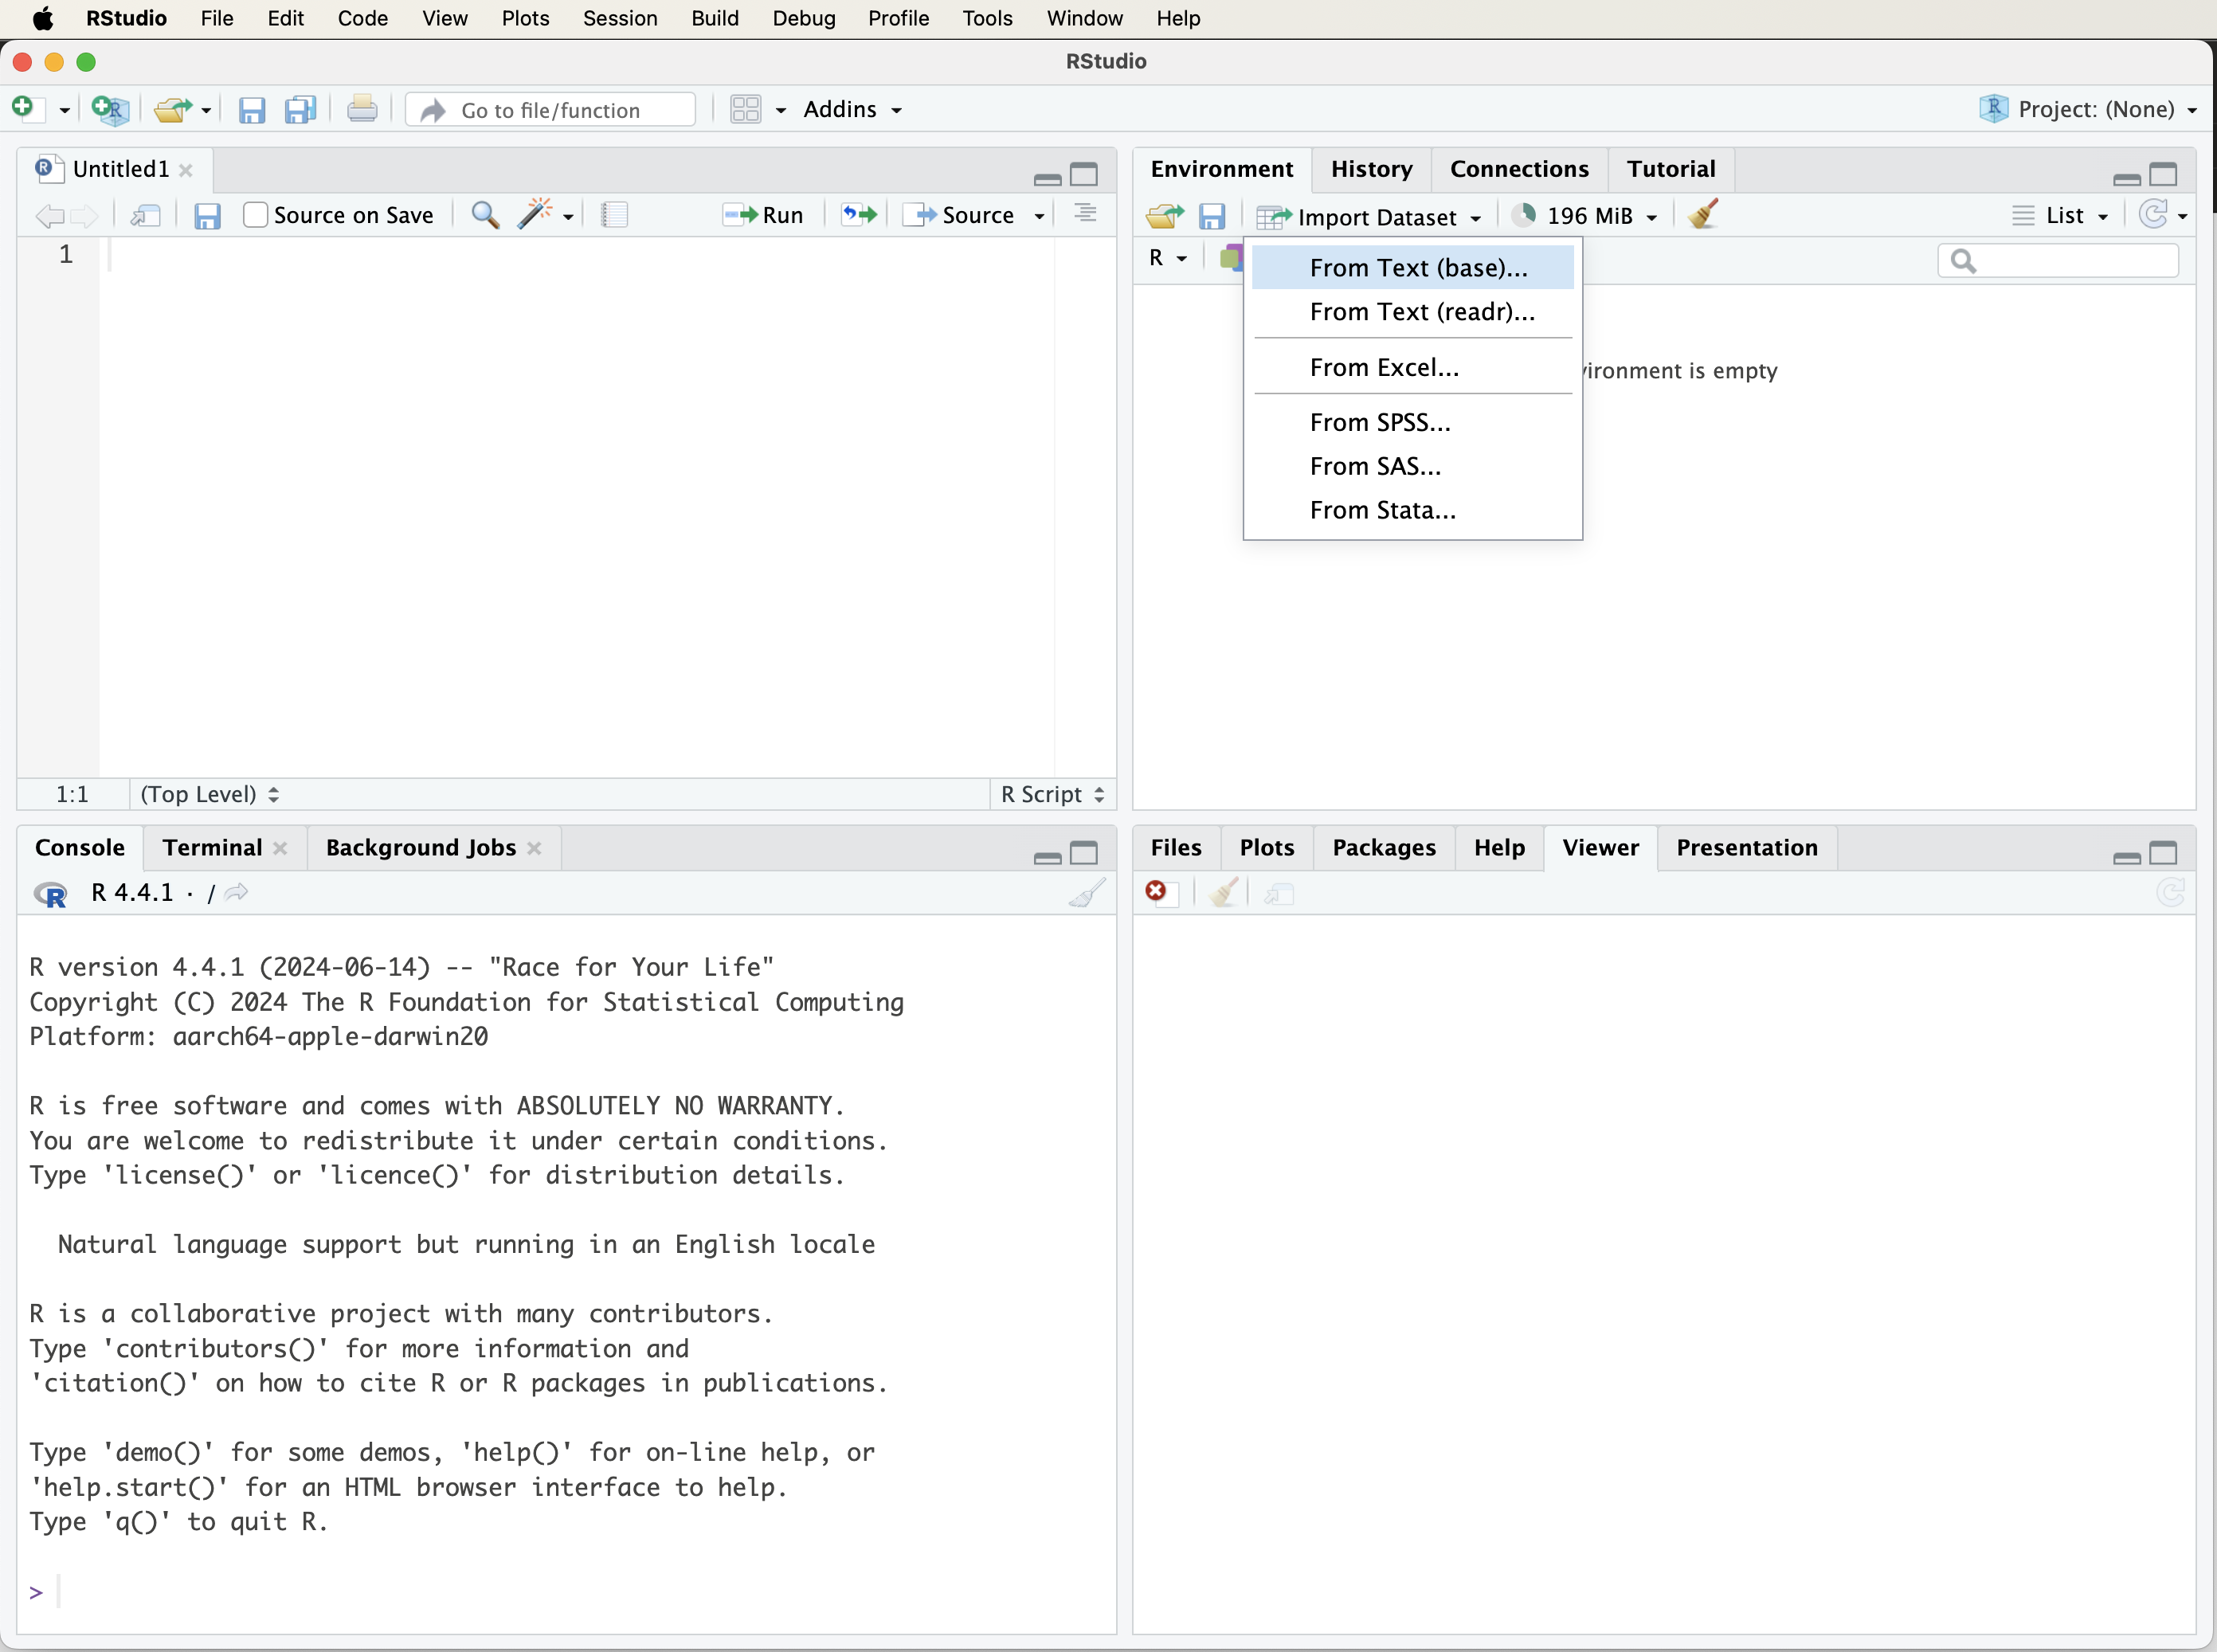
\includegraphics[width=0.7\linewidth]{images/RStudio-window-data-1} 

}

\caption{A visual guide to loading a dataset into R using the 'Import Dataset' tab in RStudio.}\label{fig:load-data}
\end{figure}

\begin{figure}

{\centering 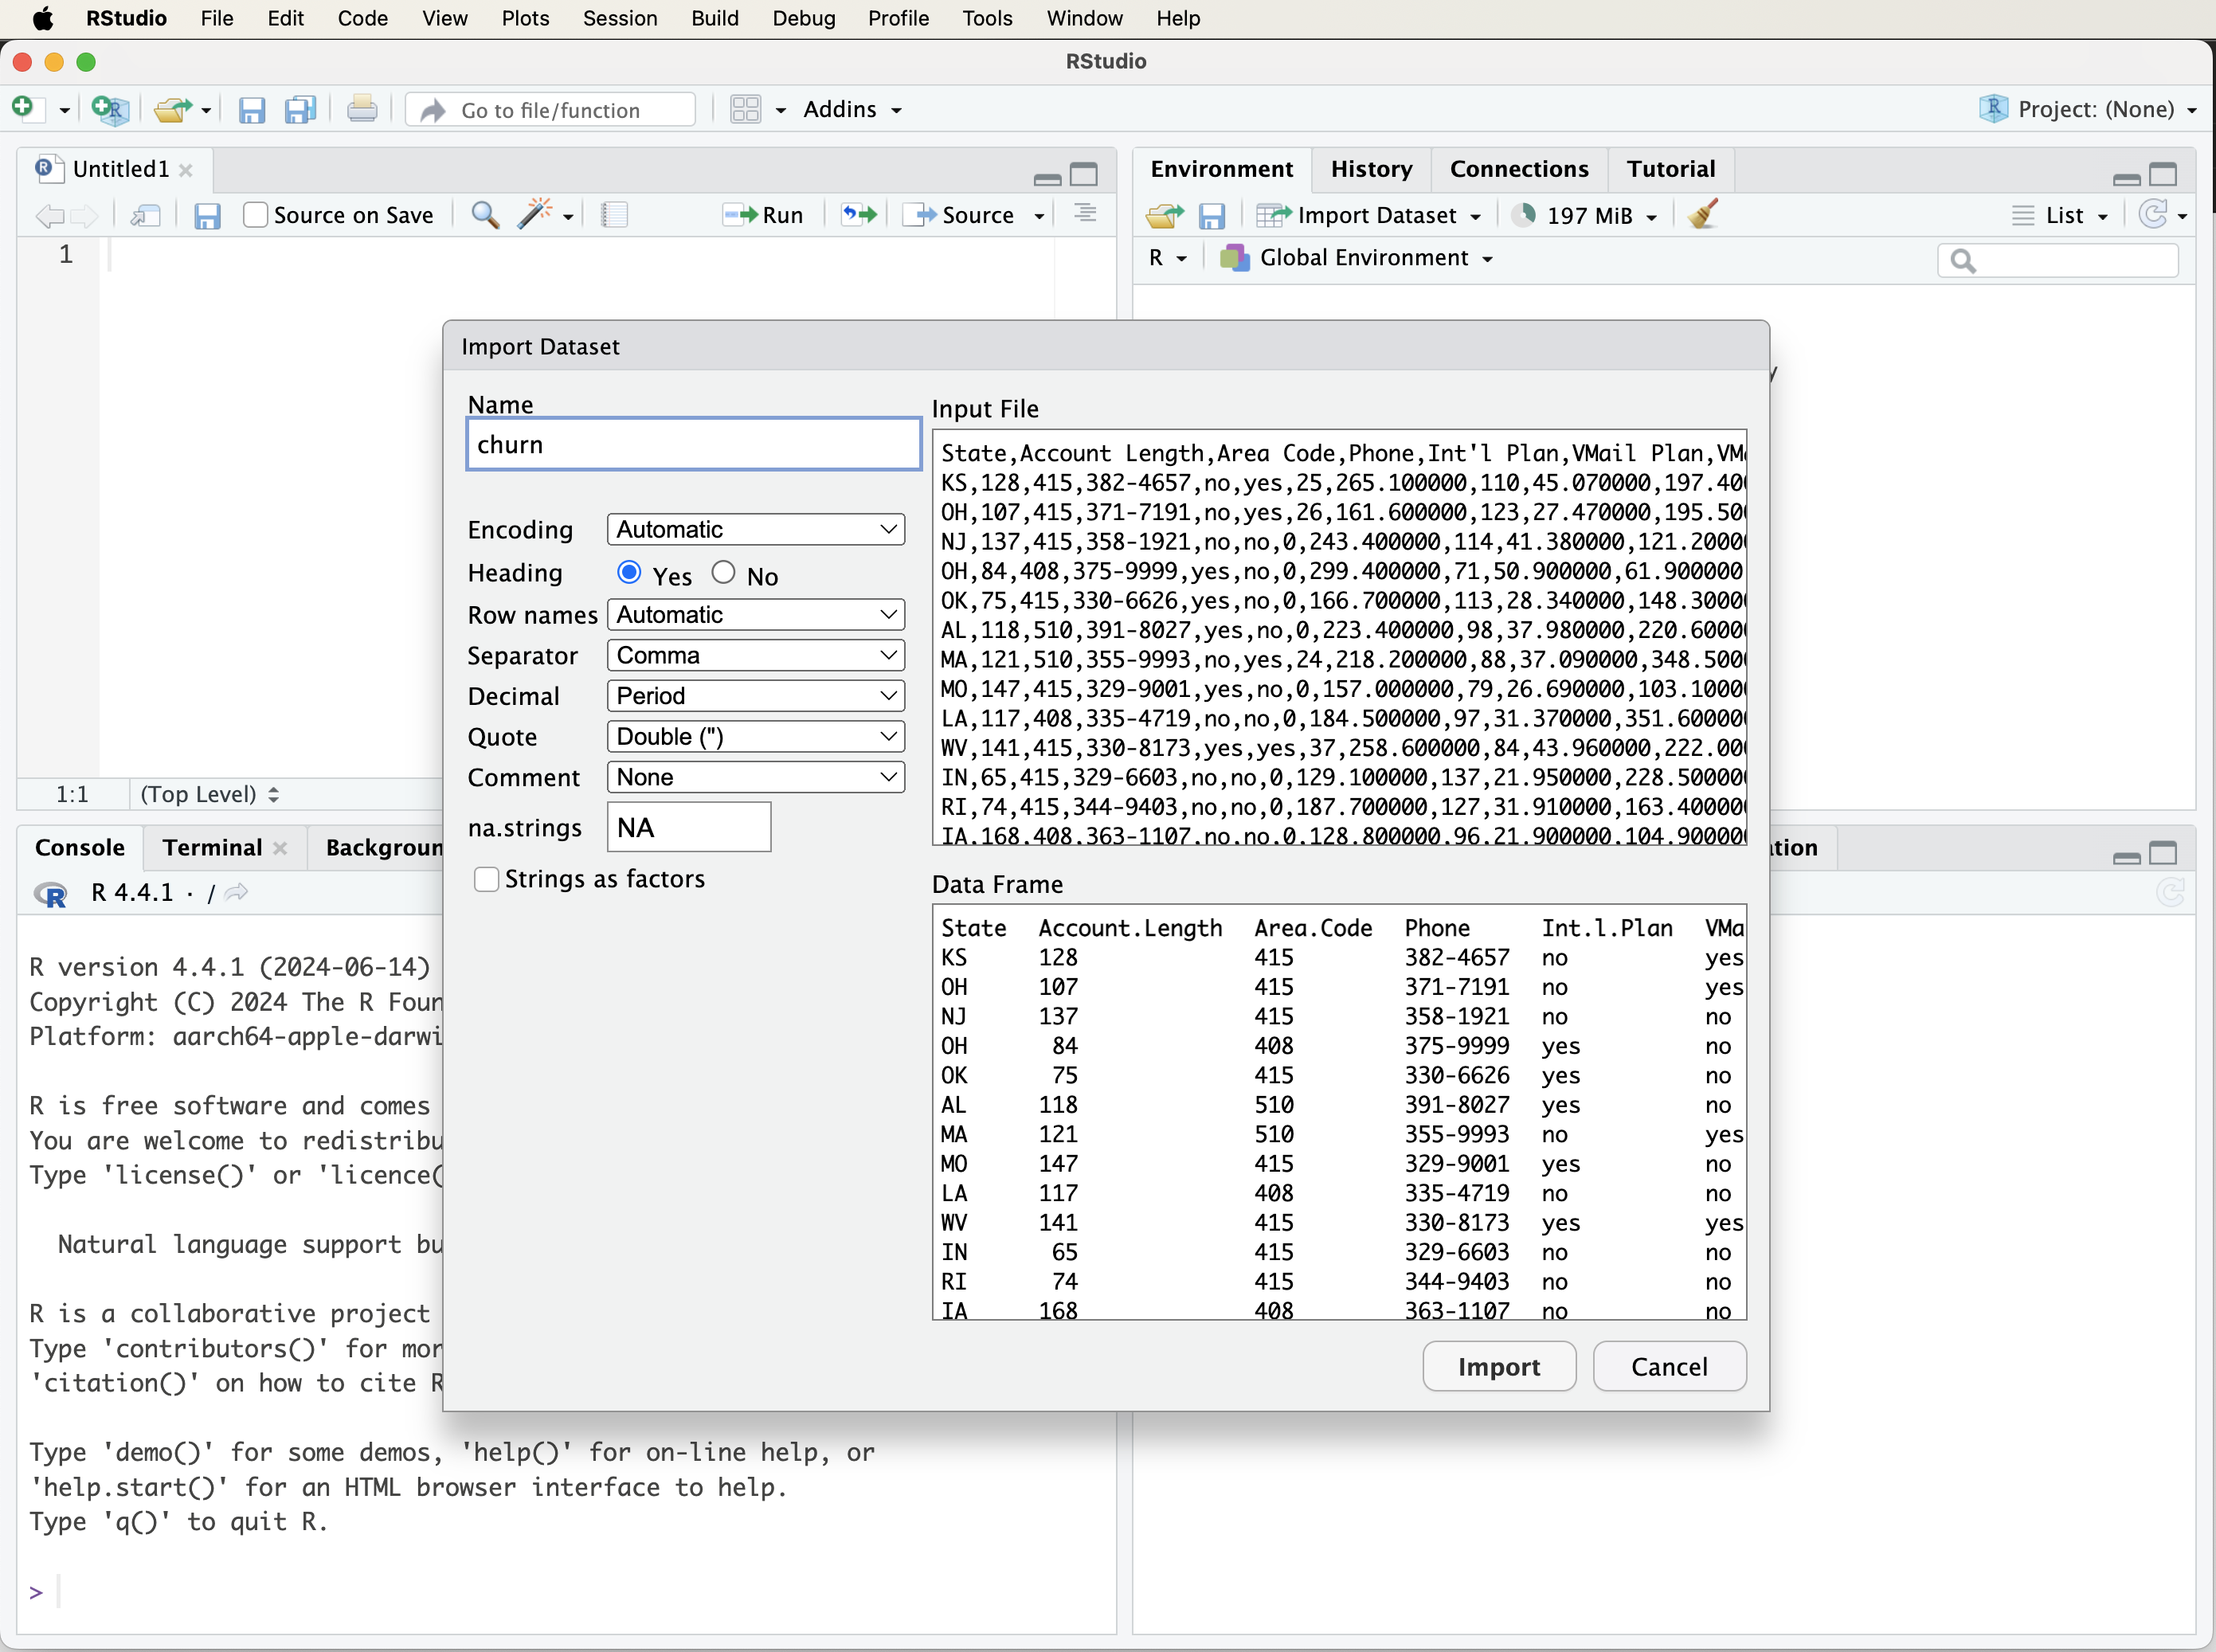
\includegraphics[width=0.7\linewidth]{images/RStudio-window-data} 

}

\caption{A visual guide to customizing the import settings when loading a dataset into R using the 'Import Dataset' tab in RStudio.}\label{fig:load-data-2}
\end{figure}

\subsection*{\texorpdfstring{Using \texttt{read.csv()}}{Using read.csv()}}\label{using-read.csv}
\addcontentsline{toc}{subsection}{Using \texttt{read.csv()}}

You can also import data directly using the \passthrough{\lstinline!read.csv()!} function, which reads tabular data (such as CSV files) into R as a data frame. If your data file is stored locally, you can load it as follows:

\begin{lstlisting}[language=R]
data <- read.csv("path/to/your/file.csv")
\end{lstlisting}

Replace \passthrough{\lstinline!"path/to/your/file.csv"!} with the actual file path. If your file does not contain column names, use:

\begin{lstlisting}[language=R]
data <- read.csv("path/to/your/file.csv", header = FALSE)
\end{lstlisting}

\subsection*{Setting the Working Directory}\label{setting-the-working-directory}
\addcontentsline{toc}{subsection}{Setting the Working Directory}

By default, R looks for files in the current working directory. If your data is located elsewhere, you can specify the full path in \passthrough{\lstinline!read.csv()!} or set the working directory.

To check your current working directory:

\begin{lstlisting}[language=R]
getwd()
\end{lstlisting}

To set a new working directory:

\begin{lstlisting}[language=R]
setwd("~/Documents")  # Adjust the path based on your system
\end{lstlisting}

Alternatively, in RStudio, go to \emph{Session \textgreater{} Set Working Directory \textgreater{} Choose Directory\ldots{}} and select the desired folder.

\subsection*{\texorpdfstring{Using \texttt{file.choose()} with \texttt{read.csv()}}{Using file.choose() with read.csv()}}\label{using-file.choose-with-read.csv}
\addcontentsline{toc}{subsection}{Using \texttt{file.choose()} with \texttt{read.csv()}}

To interactively select a file instead of typing its path manually, use \passthrough{\lstinline!file.choose()!}:

\begin{lstlisting}[language=R]
data <- read.csv(file.choose())
\end{lstlisting}

This will open a file selection dialog, making it a convenient option when working with multiple datasets.

\subsection*{Loading Data from Online Sources}\label{loading-data-from-online-sources}
\addcontentsline{toc}{subsection}{Loading Data from Online Sources}

R also allows direct import of datasets from web sources. For example, to load a publicly available COVID-19 dataset:

\begin{lstlisting}[language=R]
corona_data <- read.csv("https://opendata.ecdc.europa.eu/covid19/casedistribution/csv", 
                        na.strings = "", fileEncoding = "UTF-8-BOM")
\end{lstlisting}

This approach is useful for accessing open datasets from research institutions or government agencies.

\subsection*{\texorpdfstring{Using \texttt{read\_excel()} for Excel Files}{Using read\_excel() for Excel Files}}\label{using-read_excel-for-excel-files}
\addcontentsline{toc}{subsection}{Using \texttt{read\_excel()} for Excel Files}

To import Excel files, use the \passthrough{\lstinline!read\_excel()!} function from the \textbf{readxl} package. First, install and load the package:

\begin{lstlisting}[language=R]
install.packages("readxl")

library(readxl)
\end{lstlisting}

Then, import the Excel file:

\begin{lstlisting}[language=R]
data <- read_excel("path/to/your/file.xlsx")
\end{lstlisting}

Unlike \passthrough{\lstinline!read.csv()!}, \passthrough{\lstinline!read\_excel()!} supports multiple sheets within an Excel file, which can be specified using the \passthrough{\lstinline!sheet!} argument.\\
\#\#\# Loading Data from R Packages \{-\}

Some datasets are available directly in R packages and do not require importing from an external file. For example, the \textbf{liver} package, developed for this book, contains multiple datasets. To access the \emph{churn} dataset:

\begin{lstlisting}[language=R]
library(liver)
data(churn)
\end{lstlisting}

Since many of the datasets used in this book are included in the \textbf{liver} package (see Table \ref{tab:data-table}), we will frequently use this package for examples and demonstrations.

This section is well-structured and clearly explains the fundamental data types in R. It is concise and informative, making it accessible to beginners while maintaining a professional tone suitable for a Springer publication. Below are some minor refinements to improve clarity, consistency, and readability.

\section{Data Types in R}\label{data-types-in-r}

Data in R can take various forms, and correctly identifying these types is essential for effective data manipulation, visualization, and analysis. Each data type has specific properties that determine how R processes it, so understanding them helps avoid errors and ensures accurate results.

Here are the most common data types in R:

\begin{itemize}
\tightlist
\item
  \textbf{Numeric}: Represents real numbers, such as \passthrough{\lstinline!3.14!} or \passthrough{\lstinline!-5.67!}. This type is used for continuous numerical values, like heights, weights, or temperatures.\\
\item
  \textbf{Integer}: Represents whole numbers without decimals, such as \passthrough{\lstinline!1!}, \passthrough{\lstinline!42!}, or \passthrough{\lstinline!-10!}. This type is useful for count-based data, such as the number of customers or items sold.\\
\item
  \textbf{Character}: Represents text or string data, such as \passthrough{\lstinline!"Data Science"!} or \passthrough{\lstinline!"R Programming"!}. This type is commonly used for categorical labels, names, and descriptive values.\\
\item
  \textbf{Logical}: Represents Boolean values: \passthrough{\lstinline!TRUE!} or \passthrough{\lstinline!FALSE!}. Logical data is often used in conditional statements and filtering operations.\\
\item
  \textbf{Factor}: Represents categorical data with predefined levels. Factors are commonly used for storing variables such as \passthrough{\lstinline!"Male"!} or \passthrough{\lstinline!"Female"!} in a dataset and are particularly useful in statistical modeling.
\end{itemize}

To check the data type of a variable, use the \passthrough{\lstinline!class()!} function. For example, to determine the type of the variable \passthrough{\lstinline!result!}, type:

\begin{lstlisting}[language=R]
class(result)
   [1] "numeric"
\end{lstlisting}

Press \emph{Enter}, and R will display the variable's data type.

Recognizing different data types is essential for choosing the right analytical and visualization techniques. As we will explore in later chapters (e.g., Chapters \ref{chapter-EDA} and \ref{chapter-statistics}), numerical and categorical variables require different approaches when performing descriptive statistics, hypothesis testing, and data visualization.

\section{Data Structures in R}\label{data-structures-in-r}

Data structures are fundamental to working with data in R. They define how data is stored and manipulated, which directly impacts the efficiency and accuracy of data analysis. The most commonly used data structures in R are vectors, matrices, data frames, and lists, as illustrated in Figure \ref{fig:load-data-2}.

\begin{figure}

{\centering 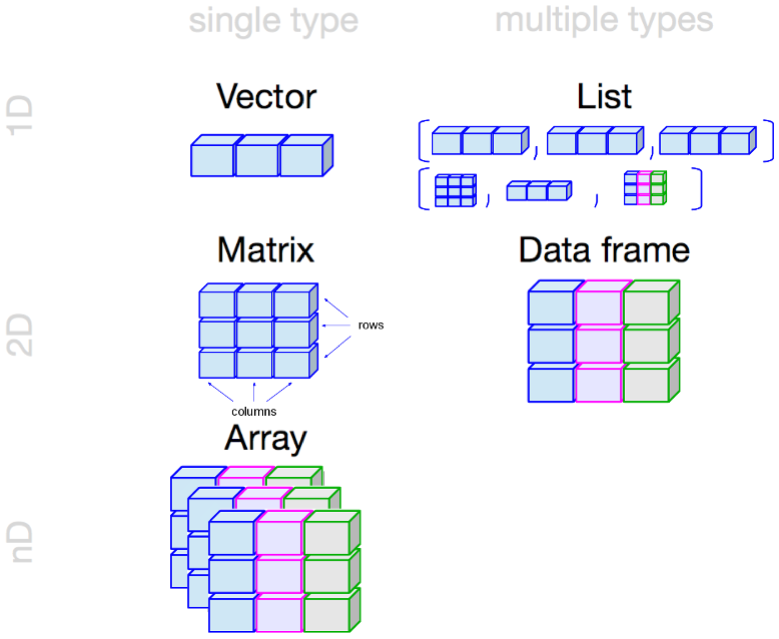
\includegraphics[width=0.6\linewidth]{images/R-objects} 

}

\caption{A visual guide to different types of data structures in R.}\label{fig:R-objects}
\end{figure}

\subsection*{Vectors in R}\label{vectors-in-r}
\addcontentsline{toc}{subsection}{Vectors in R}

A vector is the simplest data structure in R. It is a one-dimensional array that holds elements of the same type (numeric, character, or logical). Vectors are the building blocks of other data structures. You can create a vector using the \passthrough{\lstinline!c()!} function:

\begin{lstlisting}[language=R]
# Create a numeric vector
x <- c(1, 2, 0, -3, 5)

# Display the vector
x
   [1]  1  2  0 -3  5

# Check if x is a vector
is.vector(x)
   [1] TRUE

# Check the length of the vector
length(x)
   [1] 5
\end{lstlisting}

Here, \passthrough{\lstinline!x!} is a numeric vector containing five elements. The \passthrough{\lstinline!is.vector()!} function confirms that \passthrough{\lstinline!x!} is indeed a vector, while \passthrough{\lstinline!length(x)!} returns the number of elements in the vector.

\subsection*{Matrices in R}\label{matrices-in-r}
\addcontentsline{toc}{subsection}{Matrices in R}

A matrix is a two-dimensional array where all elements must be of the same type. Matrices are useful for mathematical operations and structured numerical data. You can create a matrix using the \passthrough{\lstinline!matrix()!} function:

\begin{lstlisting}[language=R]
# Create a matrix with 2 rows and 3 columns
m <- matrix(c(1, 2, 3, 4, 5, 6), nrow = 2, ncol = 3, byrow = TRUE)

# Display the matrix
m
        [,1] [,2] [,3]
   [1,]    1    2    3
   [2,]    4    5    6

# Check if m is a matrix
is.matrix(m)
   [1] TRUE

# Check the dimensions of the matrix
dim(m)
   [1] 2 3
\end{lstlisting}

This matrix \passthrough{\lstinline!m!} consists of two rows and three columns, filled row-wise. The \passthrough{\lstinline!dim()!} function returns the dimensions of the matrix. To fill the matrix column-wise, set \passthrough{\lstinline!byrow = FALSE!}.

\subsection*{Data Frames in R}\label{data-frames-in-r}
\addcontentsline{toc}{subsection}{Data Frames in R}

A data frame is a two-dimensional table where each column can contain a different data type (numeric, character, or logical). This makes data frames ideal for storing tabular data, similar to spreadsheets. You can create a data frame using the \passthrough{\lstinline!data.frame()!} function:

\begin{lstlisting}[language=R]
# Create vectors for student data
student_id <- c(101, 102, 103, 104)
name       <- c("Emma", "Bob", "Alice", "Noah")
age        <- c(20, 21, 19, 22)
grade      <- c("A", "B", "A", "C")

# Create a data frame from the vectors
students_df <- data.frame(student_id, name, age, grade)

# Display the data frame
students_df
     student_id  name age grade
   1        101  Emma  20     A
   2        102   Bob  21     B
   3        103 Alice  19     A
   4        104  Noah  22     C
\end{lstlisting}

This data frame \passthrough{\lstinline!students\_df!} consists of four columns: \passthrough{\lstinline!student\_id!}, \passthrough{\lstinline!name!}, \passthrough{\lstinline!age!}, and \passthrough{\lstinline!grade!}. The \passthrough{\lstinline!class()!} function confirms that an object is a data frame, while \passthrough{\lstinline!is.data.frame()!} checks its structure.

To inspect the first few rows of a data frame, use the \passthrough{\lstinline!head()!} function. For example, to display the first six rows of the \emph{churn} dataset from the \textbf{liver} package:

\begin{lstlisting}[language=R]
library(liver)  # Load the liver package
data(churn)     # Load the churn dataset

# Check the structure of the dataset
str(churn)
   'data.frame':    5000 obs. of  20 variables:
    $ state         : Factor w/ 51 levels "AK","AL","AR",..: 17 36 32 36 37 2 20 25 19 50 ...
    $ area.code     : Factor w/ 3 levels "area_code_408",..: 2 2 2 1 2 3 3 2 1 2 ...
    $ account.length: int  128 107 137 84 75 118 121 147 117 141 ...
    $ voice.plan    : Factor w/ 2 levels "yes","no": 1 1 2 2 2 2 1 2 2 1 ...
    $ voice.messages: int  25 26 0 0 0 0 24 0 0 37 ...
    $ intl.plan     : Factor w/ 2 levels "yes","no": 2 2 2 1 1 1 2 1 2 1 ...
    $ intl.mins     : num  10 13.7 12.2 6.6 10.1 6.3 7.5 7.1 8.7 11.2 ...
    $ intl.calls    : int  3 3 5 7 3 6 7 6 4 5 ...
    $ intl.charge   : num  2.7 3.7 3.29 1.78 2.73 1.7 2.03 1.92 2.35 3.02 ...
    $ day.mins      : num  265 162 243 299 167 ...
    $ day.calls     : int  110 123 114 71 113 98 88 79 97 84 ...
    $ day.charge    : num  45.1 27.5 41.4 50.9 28.3 ...
    $ eve.mins      : num  197.4 195.5 121.2 61.9 148.3 ...
    $ eve.calls     : int  99 103 110 88 122 101 108 94 80 111 ...
    $ eve.charge    : num  16.78 16.62 10.3 5.26 12.61 ...
    $ night.mins    : num  245 254 163 197 187 ...
    $ night.calls   : int  91 103 104 89 121 118 118 96 90 97 ...
    $ night.charge  : num  11.01 11.45 7.32 8.86 8.41 ...
    $ customer.calls: int  1 1 0 2 3 0 3 0 1 0 ...
    $ churn         : Factor w/ 2 levels "yes","no": 2 2 2 2 2 2 2 2 2 2 ...

# Display the first six rows
head(churn)
     state     area.code account.length voice.plan voice.messages intl.plan
   1    KS area_code_415            128        yes             25        no
   2    OH area_code_415            107        yes             26        no
   3    NJ area_code_415            137         no              0        no
   4    OH area_code_408             84         no              0       yes
   5    OK area_code_415             75         no              0       yes
   6    AL area_code_510            118         no              0       yes
     intl.mins intl.calls intl.charge day.mins day.calls day.charge eve.mins
   1      10.0          3        2.70    265.1       110      45.07    197.4
   2      13.7          3        3.70    161.6       123      27.47    195.5
   3      12.2          5        3.29    243.4       114      41.38    121.2
   4       6.6          7        1.78    299.4        71      50.90     61.9
   5      10.1          3        2.73    166.7       113      28.34    148.3
   6       6.3          6        1.70    223.4        98      37.98    220.6
     eve.calls eve.charge night.mins night.calls night.charge customer.calls churn
   1        99      16.78      244.7          91        11.01              1    no
   2       103      16.62      254.4         103        11.45              1    no
   3       110      10.30      162.6         104         7.32              0    no
   4        88       5.26      196.9          89         8.86              2    no
   5       122      12.61      186.9         121         8.41              3    no
   6       101      18.75      203.9         118         9.18              0    no
\end{lstlisting}

This code loads the \textbf{liver} package, retrieves the \emph{churn} dataset, and provides an overview of its structure. The \passthrough{\lstinline!str()!} function is particularly useful for summarizing data frames, as it displays data types and column values.

\subsection*{Lists in R}\label{lists-in-r}
\addcontentsline{toc}{subsection}{Lists in R}

A list is a flexible data structure that can contain elements of different types, including vectors, matrices, data frames, or even other lists. Lists are useful for storing complex objects in a structured way. You can create a list using the \passthrough{\lstinline!list()!} function:

\begin{lstlisting}[language=R]
# Create a list containing a vector, matrix, and data frame
my_list <- list(vector = x, matrix = m, data_frame = students_df)

# Display the list
my_list
   $vector
   [1]  1  2  0 -3  5
   
   $matrix
        [,1] [,2] [,3]
   [1,]    1    2    3
   [2,]    4    5    6
   
   $data_frame
     student_id  name age grade
   1        101  Emma  20     A
   2        102   Bob  21     B
   3        103 Alice  19     A
   4        104  Noah  22     C
\end{lstlisting}

This list \passthrough{\lstinline!my\_list!} stores a vector, a matrix, and a data frame within a single object. Lists allow for efficient organization of heterogeneous data. To explore the structure of a list, use the \passthrough{\lstinline!str()!} function:

\begin{lstlisting}[language=R]
str(my_list)
   List of 3
    $ vector    : num [1:5] 1 2 0 -3 5
    $ matrix    : num [1:2, 1:3] 1 4 2 5 3 6
    $ data_frame:'data.frame':  4 obs. of  4 variables:
     ..$ student_id: num [1:4] 101 102 103 104
     ..$ name      : chr [1:4] "Emma" "Bob" "Alice" "Noah"
     ..$ age       : num [1:4] 20 21 19 22
     ..$ grade     : chr [1:4] "A" "B" "A" "C"
\end{lstlisting}

Lists are powerful tools in R, especially for handling nested or hierarchical data. For further exploration, use \passthrough{\lstinline!?list!} to access the documentation and additional examples.

\section{Accessing Records or Variables in R}\label{accessing-records-or-variables-in-r}

Once you've imported data into R, you can easily access specific records or variables using the \passthrough{\lstinline!$!} and \passthrough{\lstinline![]!} operators. These tools are essential for extracting data from data frames and lists.

The \passthrough{\lstinline!$!} operator allows you to extract a specific column from a data frame or a specific element from a list. For example, to access the \passthrough{\lstinline!name!} column in the \passthrough{\lstinline!students\_df!} data frame, you would use:

\begin{lstlisting}[language=R]
students_df$name
   [1] "Emma"  "Bob"   "Alice" "Noah"
\end{lstlisting}

This command retrieves and displays the \passthrough{\lstinline!name!} column from the \passthrough{\lstinline!students\_df!} data frame.

Similarly, you can use the \passthrough{\lstinline!$!} operator to access elements within a list. For example, to access the \passthrough{\lstinline!vector!} element in the \passthrough{\lstinline!my\_list!} list:

\begin{lstlisting}[language=R]
my_list$vector
   [1]  1  2  0 -3  5
\end{lstlisting}

This command retrieves and displays the \passthrough{\lstinline!vector!} element from the \passthrough{\lstinline!my\_list!} list. The \passthrough{\lstinline!$!} operator is a straightforward and powerful way to access specific variables or elements within data frames and lists.

Another method for accessing specific records or variables is through the \passthrough{\lstinline![]!} operator, which allows you to subset data frames, matrices, and lists based on specific conditions. For example, to extract the first three rows of the \passthrough{\lstinline!students\_df!} data frame, you can use:

\begin{lstlisting}[language=R]
students_df[1:3, ]
     student_id  name age grade
   1        101  Emma  20     A
   2        102   Bob  21     B
   3        103 Alice  19     A
\end{lstlisting}

This command will display the first three rows of the \passthrough{\lstinline!students\_df!} data frame.

You can also use the \passthrough{\lstinline![]!} operator to extract specific columns. For instance, to select the \passthrough{\lstinline!name!} and \passthrough{\lstinline!grade!} columns from the \passthrough{\lstinline!students\_df!} data frame:

\begin{lstlisting}[language=R]
students_df[, c("name", "grade")]
      name grade
   1  Emma     A
   2   Bob     B
   3 Alice     A
   4  Noah     C
\end{lstlisting}

This command retrieves and displays only the \passthrough{\lstinline!name!} and \passthrough{\lstinline!grade!} columns from the \passthrough{\lstinline!students\_df!} data frame.

The \passthrough{\lstinline![]!} operator is versatile, enabling you to subset data frames, matrices, and lists with precision. Both the \passthrough{\lstinline!$!} and \passthrough{\lstinline![]!} operators are fundamental tools for data manipulation in R, allowing you to efficiently access and manage the data you need.

\section{Visualizing Data in R}\label{visualizing-data-in-r}

Data visualization is a powerful tool for exploring and communicating insights from data. It plays a crucial role in exploratory data analysis (EDA), which we will delve into in Chapter \ref{chapter-EDA}. As the saying goes, ``a picture is worth a thousand words,'' and in data science, this is especially true. R provides a broad array of tools for creating high-quality plots and visualizations, allowing you to effectively present your findings.

In R, there are two primary ways to create plots: using base R graphics and using the \textbf{ggplot2} package. Base R graphics offer a simple and direct way to generate plots, while \textbf{ggplot2} provides greater flexibility and customization. This book primarily uses \textbf{ggplot2}, as it follows a structured approach based on the \emph{grammar of graphics}, which breaks down plots into three key components:

\begin{itemize}
\tightlist
\item
  Data: The dataset to be visualized, which should be in a data frame format when using \textbf{ggplot2}.\\
\item
  Aesthetics: The visual properties of the data points, such as color, shape, and size.\\
\item
  Geometries: The type of plot to be created, such as scatter plots, bar plots, or line plots.
\end{itemize}

To create a plot using \textbf{ggplot2}, first install and load the package. Instructions for installing packages are provided in Section \ref{install-packages}. To load \textbf{ggplot2}, use the following command:

\begin{lstlisting}[language=R]
library(ggplot2)
\end{lstlisting}

Next, define the data, aesthetics, and geometries for your plot. For example, to create a scatter plot of miles per gallon (\passthrough{\lstinline!mpg!}) versus horsepower (\passthrough{\lstinline!hp!}) using the built-in \emph{mtcars} dataset:

\begin{lstlisting}[language=R]
ggplot(data = mtcars) +
  geom_point(mapping = aes(x = mpg, y = hp))
\end{lstlisting}

\begin{center}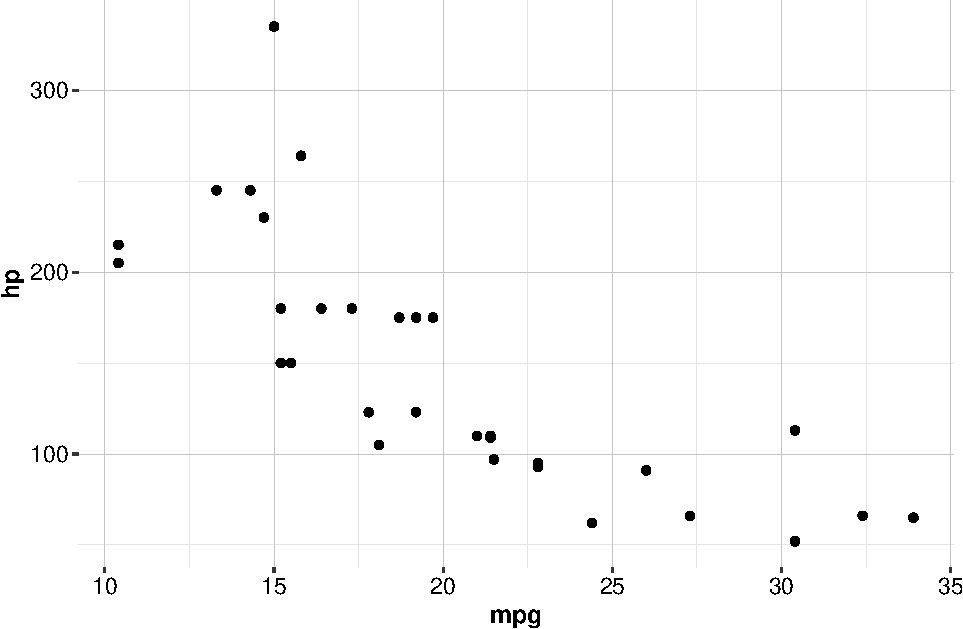
\includegraphics{Intro-R_files/figure-latex/unnamed-chunk-32-1} \end{center}

This code initializes the plot with the \passthrough{\lstinline!ggplot()!} function, specifying the dataset (\passthrough{\lstinline!mtcars!}). The \passthrough{\lstinline!geom\_point()!} function adds points to the plot, and the \passthrough{\lstinline!aes()!} function maps \passthrough{\lstinline!mpg!} to the x-axis and \passthrough{\lstinline!hp!} to the y-axis.

The general template for creating plots with \textbf{ggplot2} follows this structure:

\begin{lstlisting}[language=R]
ggplot(data = <DATA>) +
  <GEOM_FUNCTION>(mapping = aes(<MAPPINGS>))
\end{lstlisting}

Using this template, a variety of visualizations can be created.

\subsection*{Geom Functions in ggplot2}\label{geom-functions-in-ggplot2}
\addcontentsline{toc}{subsection}{Geom Functions in ggplot2}

Geom functions determine the type of plot created in \textbf{ggplot2}. Some commonly used geom functions include:

\begin{itemize}
\tightlist
\item
  \passthrough{\lstinline!geom\_point()!} for scatter plots\\
\item
  \passthrough{\lstinline!geom\_bar()!} for bar plots\\
\item
  \passthrough{\lstinline!geom\_line()!} for line plots\\
\item
  \passthrough{\lstinline!geom\_boxplot()!} for box plots\\
\item
  \passthrough{\lstinline!geom\_histogram()!} for histograms\\
\item
  \passthrough{\lstinline!geom\_density()!} for density plots\\
\item
  \passthrough{\lstinline!geom\_smooth()!} for adding smoothed conditional means to plots
\end{itemize}

For example, to create a smoothed line plot of \passthrough{\lstinline!mpg!} versus \passthrough{\lstinline!hp!}:

\begin{lstlisting}[language=R]
ggplot(data = mtcars) +
  geom_smooth(mapping = aes(x = mpg, y = hp))
\end{lstlisting}

\begin{center}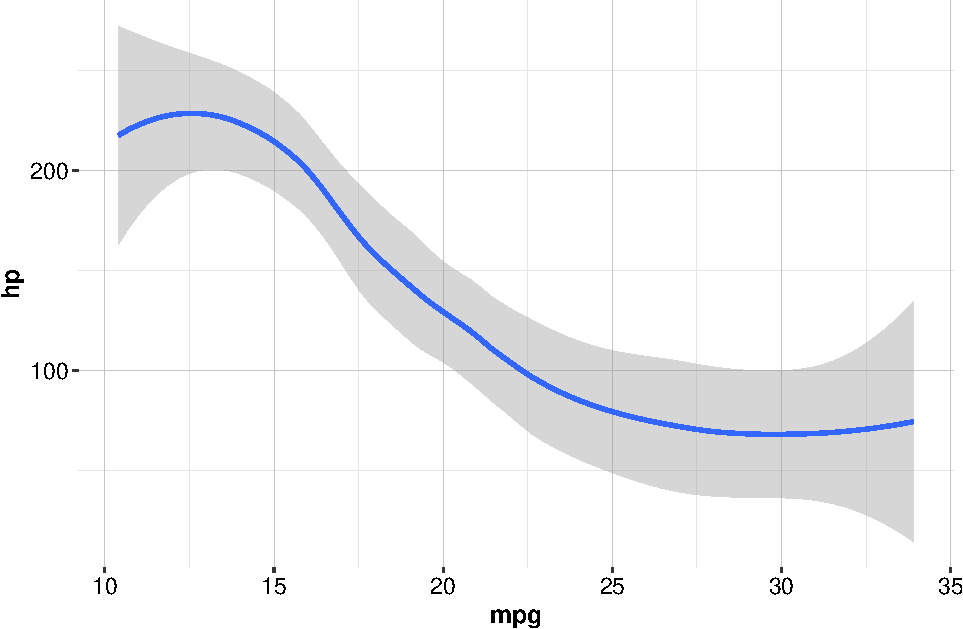
\includegraphics{Intro-R_files/figure-latex/unnamed-chunk-34-1} \end{center}

Multiple geom functions can be combined in a single plot. To overlay a scatter plot on the smoothed line:

\begin{lstlisting}[language=R]
ggplot(data = mtcars) +
  geom_smooth(mapping = aes(x = mpg, y = hp)) + 
  geom_point(mapping = aes(x = mpg, y = hp))
\end{lstlisting}

\begin{center}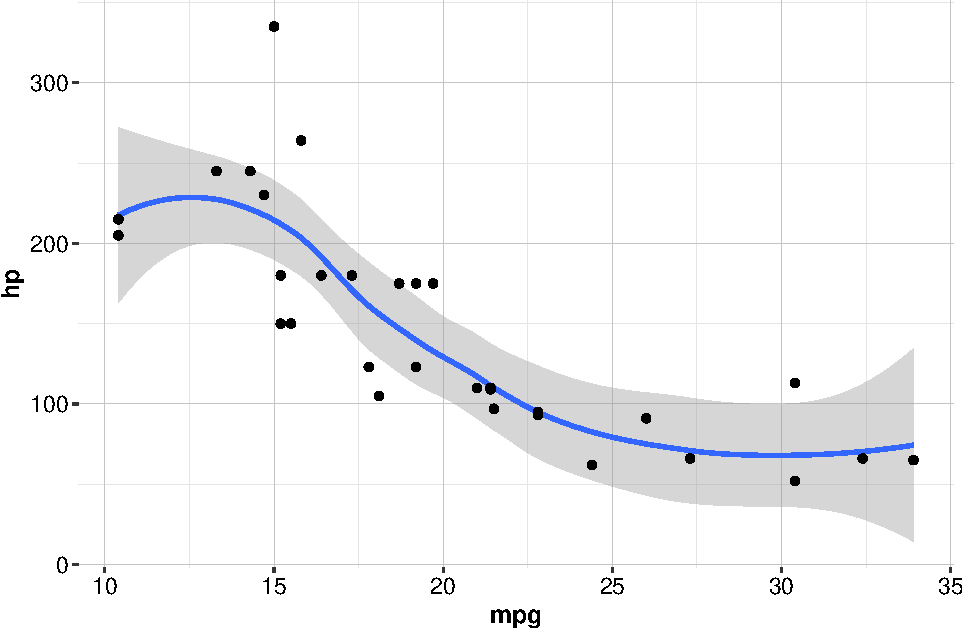
\includegraphics{Intro-R_files/figure-latex/unnamed-chunk-35-1} \end{center}

Alternatively, the \passthrough{\lstinline!aes()!} function can be placed inside \passthrough{\lstinline!ggplot()!} to streamline the code:

\begin{lstlisting}[language=R]
ggplot(data = mtcars, mapping = aes(x = mpg, y = hp)) +
  geom_smooth() + 
  geom_point()
\end{lstlisting}

Additional visualization examples can be found in Chapter \ref{chapter-EDA}. For a complete list of geom functions, refer to the \href{https://ggplot2.tidyverse.org}{\textbf{ggplot2} documentation}.

\subsection*{Aesthetics in ggplot2}\label{aesthetics-in-ggplot2}
\addcontentsline{toc}{subsection}{Aesthetics in ggplot2}

Aesthetics control the visual properties of data points, such as color, size, and shape. These properties are specified within the \passthrough{\lstinline!aes()!} function. For example:

\begin{lstlisting}[language=R]
ggplot(data = mtcars) +
  geom_point(mapping = aes(x = mpg, y = hp, color = cyl))
\end{lstlisting}

\begin{center}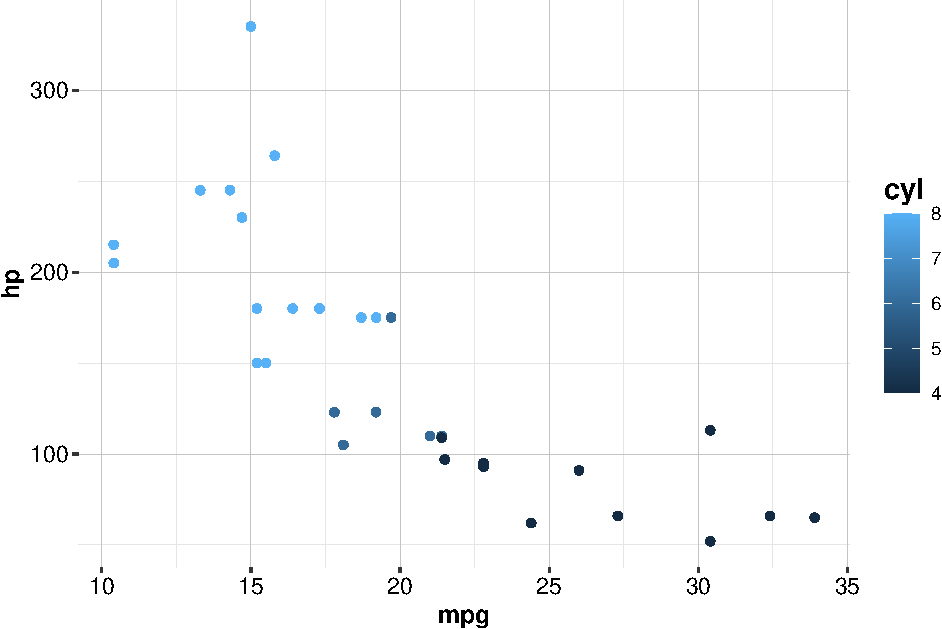
\includegraphics{Intro-R_files/figure-latex/unnamed-chunk-37-1} \end{center}

Here, \passthrough{\lstinline!color = cyl!} maps the color of the points to the number of cylinders (\passthrough{\lstinline!cyl!}) in the \textbf{mtcars} dataset. \textbf{ggplot2} automatically assigns a unique color to each category and adds a corresponding legend.

In addition to \passthrough{\lstinline!color!}, other aesthetics such as \passthrough{\lstinline!size!} and \passthrough{\lstinline!alpha!} (transparency) can be used:

\begin{lstlisting}[language=R]
# Left plot: using the size aesthetic
ggplot(data = mtcars) +
  geom_point(mapping = aes(x = mpg, y = hp, size = cyl))

# Right plot: using the alpha aesthetic
ggplot(data = mtcars) +
  geom_point(mapping = aes(x = mpg, y = hp, alpha = cyl))
\end{lstlisting}

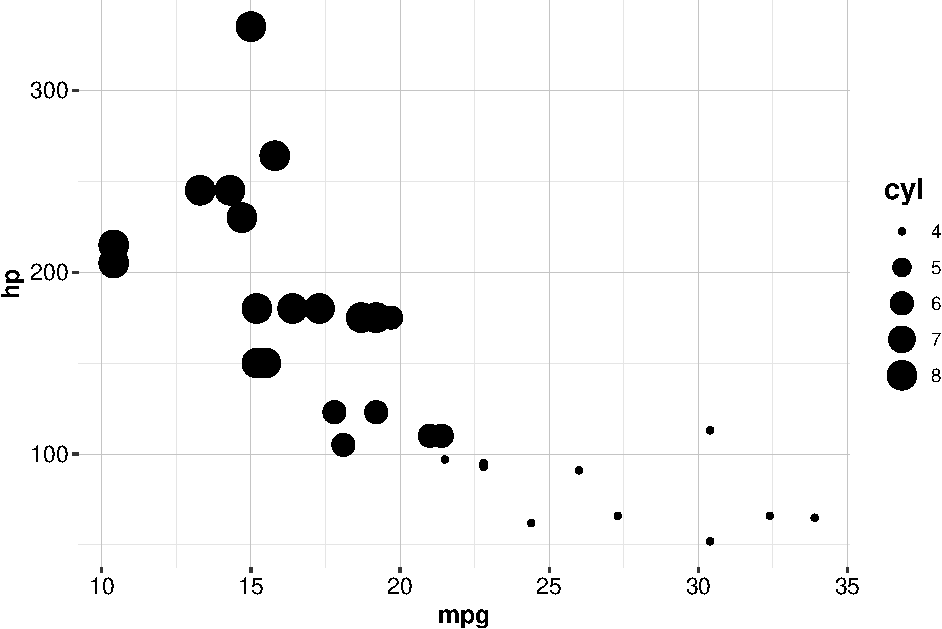
\includegraphics[width=0.5\linewidth]{Intro-R_files/figure-latex/unnamed-chunk-38-1} 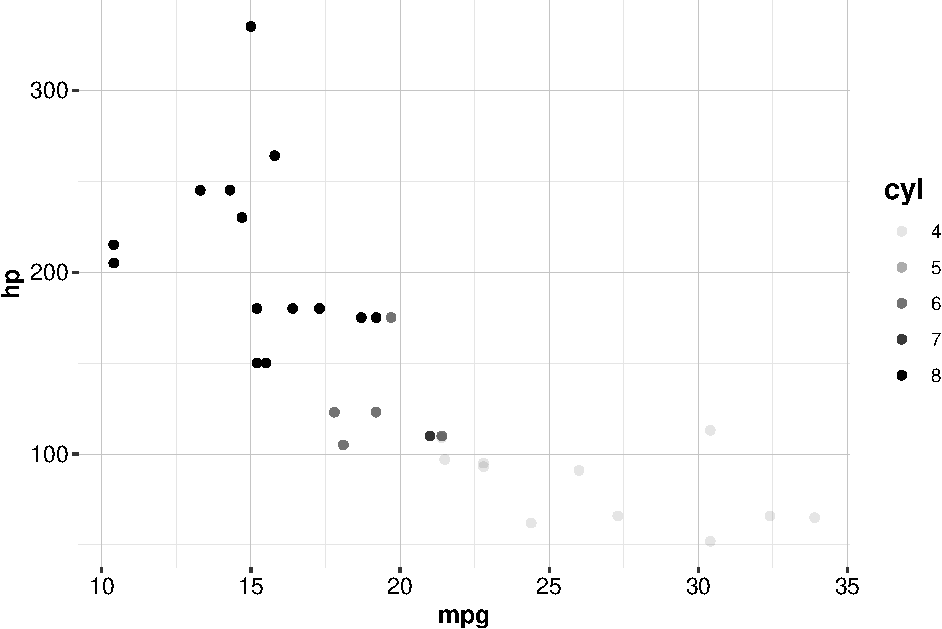
\includegraphics[width=0.5\linewidth]{Intro-R_files/figure-latex/unnamed-chunk-38-2}

Aesthetics can also be set directly inside geom functions. For example, to make all points blue triangles of size 3:

\begin{lstlisting}[language=R]
ggplot(data = mtcars) +
  geom_point(mapping = aes(x = mpg, y = hp), 
             color = "blue", size = 3, shape = 2)
\end{lstlisting}

\begin{center}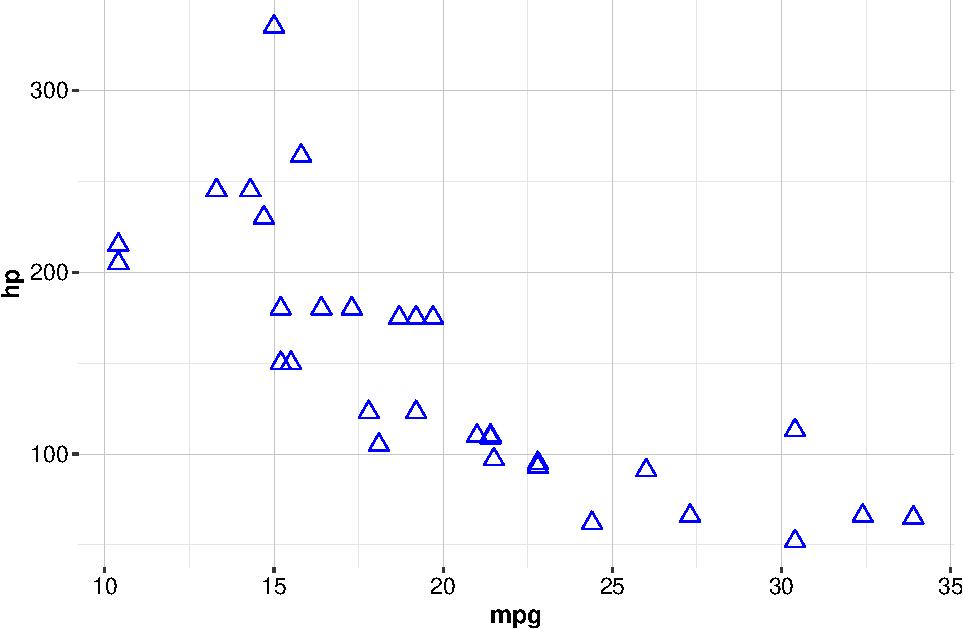
\includegraphics{Intro-R_files/figure-latex/unnamed-chunk-39-1} \end{center}

This section introduced the fundamentals of data visualization in R using \textbf{ggplot2}. The next chapters will explore how visualization plays a crucial role in exploratory data analysis (Chapter \ref{chapter-EDA}) and how to refine plots for communication and reporting. For more details on visualization techniques, see the \href{https://ggplot2.tidyverse.org}{\textbf{ggplot2} documentation}. For interactive graphics, consider exploring the \textbf{plotly} package or \textbf{Shiny} for web applications.

\section{Formula in R}\label{sec-formula-in-R}

Formulas in R provide a concise and intuitive way to specify relationships between variables for statistical modeling. They are widely used in functions for regression, classification, and machine learning to define how a response variable depends on one or more predictors.

In R, formulas use the tilde symbol \passthrough{\lstinline!\~!} to express relationships between variables, where the response variable appears on the left-hand side and predictor variables on the right-hand side. For example, the formula \passthrough{\lstinline!y \~ x!} specifies that \passthrough{\lstinline!y!} is modeled as a function of \passthrough{\lstinline!x!}. When there are multiple predictors, they are separated by \passthrough{\lstinline!+!}.\\
For instance, using the \passthrough{\lstinline!diamonds!} dataset, the formula:

\begin{lstlisting}[language=R]
price ~ carat + cut + color
\end{lstlisting}

models the \passthrough{\lstinline!price!} of a diamond based on its \passthrough{\lstinline!carat!}, \passthrough{\lstinline!cut!}, and \passthrough{\lstinline!color!}.

To include all other variables in the dataset as predictors, we can use the shorthand notation:

\begin{lstlisting}[language=R]
price ~ .
\end{lstlisting}

This approach is particularly useful in large datasets where listing all predictors manually would be impractical.

A formula in R acts as a \textbf{quoting operator}, instructing R to interpret the variables symbolically rather than evaluating them immediately. The variable on the left-hand side of \passthrough{\lstinline!\~!} is the \textbf{dependent variable} (or response variable), while the variables on the right-hand side are the \textbf{independent variables} (or predictor variables).

\begin{example}
\protect\hypertarget{exm:ex-formula}{}\label{exm:ex-formula}To illustrate, suppose we want to predict the \passthrough{\lstinline!price!} of a diamond using a linear regression model. We can pass the formula into the \passthrough{\lstinline!lm()!} function:

\begin{lstlisting}[language=R]
model <- lm(price ~ carat + cut + color, data = diamonds)
\end{lstlisting}

Here, the formula \passthrough{\lstinline!price \~ carat + cut + color!} defines the relationship, and the \passthrough{\lstinline!data!} argument specifies the dataset to use.
\end{example}

Once defined, formulas can be used in various R functions for statistical modeling and machine learning. As you progress through later chapters, you will encounter formulas in functions for regression, classification, and more (e.g., Chapters \ref{chapter-knn}, \ref{chapter-bayes}, and \ref{chapter-regression}). Mastering formula syntax will enable you to efficiently build, customize, and interpret models throughout this book.

\section{Reporting with R Markdown}\label{reporting-with-r-markdown}

Thus far, this book has covered how to interact with R and RStudio for data analysis. This section focuses on an equally important aspect: effectively communicating analytical findings. Data scientists must present results clearly to teams, stakeholders, and clients. Regardless of the depth of an analysis, its impact is limited if it is not communicated effectively. R Markdown facilitates this process by enabling the seamless integration of code, text, and output into dynamic, reproducible reports.

R Markdown allows users to write and execute R code within a document, producing reports, presentations, and dashboards. It employs Markdown, a lightweight markup language designed for ease of reading and writing. This entire book was written in R Markdown, with all source files available on GitHub. R Markdown streamlines report generation, ensuring that text, code, and visualizations remain synchronized as data changes.

R Markdown documents can be exported into multiple formats, including HTML, PDF, Word, and PowerPoint, making it adaptable to various audiences and reporting needs. Furthermore, it supports the creation of interactive documents using Shiny, allowing users to build web applications that facilitate exploratory data analysis.

To get started, the following resources provide useful references:

\begin{itemize}
\tightlist
\item
  \textbf{R Markdown Cheat Sheet}: The \href{https://rstudio.com/wp-content/uploads/2016/03/rmarkdown-cheatsheet-2.0.pdf}{R Markdown Cheat Sheet} offers a concise reference for creating documents, including syntax, formatting, and output options. It is available in RStudio under \emph{Help \textgreater{} Cheatsheets \textgreater{} R Markdown Cheat Sheet}.\\
\item
  \textbf{R Markdown Reference Guide}: The \href{https://rstudio.com/wp-content/uploads/2015/03/rmarkdown-reference.pdf}{R Markdown Reference Guide} provides a detailed overview of R Markdown's features, including document structure and customization.
\end{itemize}

\subsection*{R Markdown Basics}\label{r-markdown-basics}
\addcontentsline{toc}{subsection}{R Markdown Basics}

R Markdown follows a literate programming approach, combining text and executable code in a single document. Unlike word processors where formatting is visible during writing, R Markdown requires compilation to generate the final report. This approach ensures automation, as plots and figures are generated dynamically and inserted into the document. Since the code is embedded, analyses are fully reproducible.

To create an R Markdown document in RStudio:

File \textgreater{} New File \textgreater{} R Markdown

A dialog box will appear, allowing the selection of a document type. For a standard report, choose ``Document.'' Other options include ``Presentation'' for slides, ``Shiny'' for interactive applications, and ``From Template'' for predefined formats. After selecting the document type, enter a title and author name. The output format can be set to HTML, PDF, or Word; HTML is often recommended for debugging.

R Markdown files use the \passthrough{\lstinline!.Rmd!} extension, distinguishing them from \passthrough{\lstinline!.R!} script files. A newly created file contains a template that can be modified with custom text, code, and formatting.

\subsection*{The Header}\label{the-header}
\addcontentsline{toc}{subsection}{The Header}

The header defines metadata such as the document's title, author, date, and output format. It is enclosed within three dashes (\passthrough{\lstinline!---!}).

\begin{lstlisting}
---
title: "An Analysis of Customer Churn"
author: "Reza Mohammadi"
date: "Aug 12, 2024"
output: html_document
---
\end{lstlisting}

\begin{itemize}
\tightlist
\item
  \textbf{Title}: The document's title.\\
\item
  \textbf{Author}: The name of the author.\\
\item
  \textbf{Date}: The date of creation.\\
\item
  \textbf{Output format}: The format of the final document (\passthrough{\lstinline!html\_document!}, \passthrough{\lstinline!pdf\_document!}, or \passthrough{\lstinline!word\_document!}).
\end{itemize}

Additional metadata can be included for customization, such as table of contents options and formatting preferences.

\subsection*{Code Chunks and Inline Code}\label{code-chunks-and-inline-code}
\addcontentsline{toc}{subsection}{Code Chunks and Inline Code}

R Markdown integrates R code within documents using code chunks, which are enclosed in triple backticks (\passthrough{\lstinline!```\{r\}!}) followed by the code. For example:

\begin{lstlisting}

```r
2 + 3
   [1] 5
```
\end{lstlisting}

When compiled, R executes the code and displays the output within the document. Code chunks are used for analysis, visualizations, and modeling. The ``Run'' button in RStudio allows individual execution of chunks. See Figure \ref{fig:run-chunk} for a visual guide.

\begin{figure}

{\centering 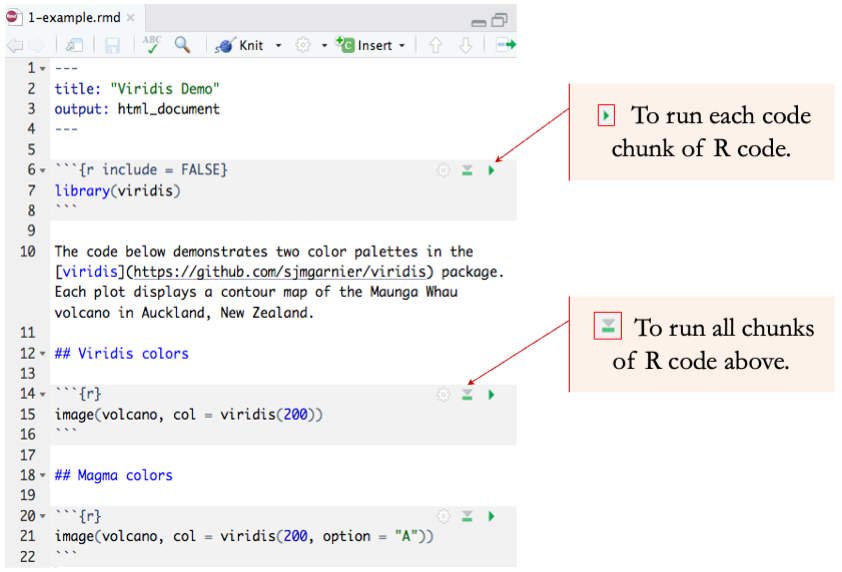
\includegraphics[width=0.9\linewidth]{images/run-chunk} 

}

\caption{Executing a code chunk in R Markdown using the 'Run' button in RStudio.}\label{fig:run-chunk}
\end{figure}

Common chunk options include:

\begin{itemize}
\tightlist
\item
  \passthrough{\lstinline!echo = FALSE!}: Displays output but hides the code.\\
\item
  \passthrough{\lstinline!eval = FALSE!}: Shows the code but does not execute it.\\
\item
  \passthrough{\lstinline!message = FALSE!}: Suppresses messages.\\
\item
  \passthrough{\lstinline!warning = FALSE!}: Suppresses warnings.\\
\item
  \passthrough{\lstinline!error = FALSE!}: Hides error messages.\\
\item
  \passthrough{\lstinline!include = FALSE!}: Omits both code and output.
\end{itemize}

For inline calculations, use backticks and the \passthrough{\lstinline!r!} keyword:

\begin{lstlisting}
The factorial of 5 is 120.
\end{lstlisting}

This renders dynamically as:

\begin{lstlisting}
The factorial of 5 is 120.
\end{lstlisting}

\subsection*{Styling Text}\label{styling-text}
\addcontentsline{toc}{subsection}{Styling Text}

R Markdown supports various text formatting options:

\begin{itemize}
\tightlist
\item
  \textbf{Headings}: Use \passthrough{\lstinline!\#!} for section titles.\\
\item
  \textbf{Bold}: Enclose text in double asterisks (\passthrough{\lstinline!**bold**!}).\\
\item
  \textbf{Italic}: Use single asterisks (\passthrough{\lstinline!*italic*!}).\\
\item
  \textbf{Lists}: Use \passthrough{\lstinline!*!} for bullet points.\\
\item
  \textbf{Links}: \passthrough{\lstinline![R Markdown website](https://rmarkdown.rstudio.com)!}\\
\item
  \textbf{Images}: \passthrough{\lstinline"![Alt text](path/to/image.png)"}
\end{itemize}

For mathematical notation, use LaTeX-style equations:

\begin{lstlisting}
Inline: $y = \beta_0 + \beta_1 x$  
Block: $$ y = \beta_0 + \beta_1 x $$
\end{lstlisting}

\subsection*{Mastering R Markdown}\label{mastering-r-markdown}
\addcontentsline{toc}{subsection}{Mastering R Markdown}

For further learning:

\begin{itemize}
\tightlist
\item
  \textbf{Books}: \href{https://bookdown.org/yihui/rmarkdown/}{\emph{R Markdown: The Definitive Guide}}.\\
\item
  \textbf{Tutorials}: \href{https://rmarkdown.rstudio.com/lesson-1.html}{R Markdown website}.\\
\item
  \textbf{Courses}: \href{https://www.datacamp.com/courses/reporting-with-r-markdown}{DataCamp R Markdown course}.\\
\item
  \textbf{Forums}: \href{https://community.rstudio.com/c/rmarkdown/9}{RStudio Community}.
\end{itemize}

By leveraging R Markdown, data scientists can produce high-quality, reproducible reports that enhance collaboration and communication.

\section{Exercises}\label{exercises}

This section provides hands-on exercises to reinforce your understanding of the fundamental concepts covered in this chapter.

\subsection*{Basic Exercises}\label{basic-exercises}
\addcontentsline{toc}{subsection}{Basic Exercises}

\begin{enumerate}
\def\labelenumi{\arabic{enumi}.}
\tightlist
\item
  Install \textbf{R} and \textbf{RStudio} on your computer.\\
\item
  Use the \passthrough{\lstinline!getwd()!} function to check your current working directory. Then, change it to a new directory using \passthrough{\lstinline!setwd()!}.\\
\item
  Install and load the \textbf{liver} package in R. If you encounter any errors, check your internet connection and ensure CRAN is accessible.\\
\item
  Create a numeric vector named \passthrough{\lstinline!numbers!} containing the values \passthrough{\lstinline!5, 10, 15, 20, 25!}. Then, calculate the mean and standard deviation of the vector.\\
\item
  Write a comment in R explaining the purpose of the following line of code:
\end{enumerate}

\begin{lstlisting}[language=R]
result <- 2 + 3
\end{lstlisting}

\begin{enumerate}
\def\labelenumi{\arabic{enumi}.}
\setcounter{enumi}{5}
\tightlist
\item
  Create a character vector containing the names of three programming languages you would like to learn. Print the vector.\\
\item
  Convert the following vector into a factor:
\end{enumerate}

\begin{lstlisting}[language=R]
cities <- c("Amsterdam", "Berlin", "London", "Amsterdam", "Berlin")
\end{lstlisting}

\begin{enumerate}
\def\labelenumi{\arabic{enumi}.}
\setcounter{enumi}{7}
\tightlist
\item
  Create a matrix with 3 rows and 4 columns, filled with numbers from 1 to 12.\\
\item
  Create a data frame containing the following variables:

  \begin{itemize}
  \tightlist
  \item
    \passthrough{\lstinline!student\_id!} (integer)\\
  \item
    \passthrough{\lstinline!name!} (character)\\
  \item
    \passthrough{\lstinline!score!} (numeric)\\
  \item
    \passthrough{\lstinline!passed!} (logical, where \passthrough{\lstinline!TRUE!} means the student passed and \passthrough{\lstinline!FALSE!} means they failed)\\
    Print the first few rows of the data frame using \passthrough{\lstinline!head()!}.\\
  \end{itemize}
\item
  Load the built-in \textbf{mtcars} dataset and display the structure of the dataset using the \passthrough{\lstinline!str()!} function.
\end{enumerate}

\subsection*{Intermediate Exercises}\label{intermediate-exercises}
\addcontentsline{toc}{subsection}{Intermediate Exercises}

\begin{enumerate}
\def\labelenumi{\arabic{enumi}.}
\setcounter{enumi}{10}
\tightlist
\item
  Import a CSV file into R using the \passthrough{\lstinline!read.csv()!} function. Print the first six rows of the dataset.\\
\item
  Create a scatter plot using \textbf{ggplot2} that visualizes the relationship between \passthrough{\lstinline!mpg!} and \passthrough{\lstinline!hp!} in the \textbf{mtcars} dataset.\\
\item
  Using the \textbf{liver} package, load the \emph{churn} dataset and display the summary statistics of the numerical variables.\\
\item
  Create a boxplot to compare the distribution of \passthrough{\lstinline!mpg!} across different values of \passthrough{\lstinline!cyl!} in the \textbf{mtcars} dataset.\\
\item
  Use the \passthrough{\lstinline!mean()!} function to compute the mean of the \passthrough{\lstinline!mpg!} variable in the \textbf{mtcars} dataset. Then, calculate the mean of \passthrough{\lstinline!mpg!} for cars with \passthrough{\lstinline!cyl == 4!}.\\
\item
  Use a formula in R to fit a linear model predicting \passthrough{\lstinline!mpg!} based on \passthrough{\lstinline!hp!} in the \textbf{mtcars} dataset. Display a summary of the model using \passthrough{\lstinline!summary()!}.\\
\item
  Create an R Markdown document that includes a title, author, and a small analysis of the \textbf{mtcars} dataset. Generate an HTML report.
\end{enumerate}

\subsection*{More Challenges Exercise}\label{more-challenges-exercise}
\addcontentsline{toc}{subsection}{More Challenges Exercise}

\begin{enumerate}
\def\labelenumi{\arabic{enumi}.}
\setcounter{enumi}{17}
\tightlist
\item
  The formula syntax in R is essential for statistical modeling. Write formulas for the following relationships:

  \begin{itemize}
  \tightlist
  \item
    A linear model predicting \passthrough{\lstinline!mpg!} using \passthrough{\lstinline!hp!} and \passthrough{\lstinline!wt!} in \textbf{mtcars}.\\
  \item
    A logistic regression model predicting \passthrough{\lstinline!vs!} using all other variables in \textbf{mtcars}.\\
  \end{itemize}
\item
  Modify the dataset below to replace the \passthrough{\lstinline!score!} column with letter grades (\passthrough{\lstinline!A!}, \passthrough{\lstinline!B!}, \passthrough{\lstinline!C!}, or \passthrough{\lstinline!D!}) based on the following rules:

  \begin{itemize}
  \tightlist
  \item
    \passthrough{\lstinline!score >= 90!}: ``A''\\
  \item
    \passthrough{\lstinline!score >= 75!}: ``B''\\
  \item
    \passthrough{\lstinline!score >= 60!}: ``C''\\
  \item
    Otherwise: ``D''
  \end{itemize}
\end{enumerate}

\begin{lstlisting}[language=R]
student_df <- data.frame(
  student_id = 1:5,
  name = c("Alice", "Bob", "Charlie", "David", "Eva"),
  score = c(95, 88, 72, 60, 45)
)
\end{lstlisting}

\begin{enumerate}
\def\labelenumi{\arabic{enumi}.}
\setcounter{enumi}{19}
\tightlist
\item
  Create a function in R that takes a numeric vector as input and returns a list containing the mean, median, and standard deviation of the vector.
\end{enumerate}

\subsection*{More Challenges Exercise}\label{more-challenges-exercise-1}
\addcontentsline{toc}{subsection}{More Challenges Exercise}

\begin{enumerate}
\def\labelenumi{\arabic{enumi}.}
\setcounter{enumi}{20}
\tightlist
\item
  The following R code generates a simulated dataset with 200 observations and three variables:

  \begin{itemize}
  \tightlist
  \item
    \passthrough{\lstinline!Age!} (numeric)\\
  \item
    \passthrough{\lstinline!Ratio!} (Sodium/Potassium ratio)\\
  \item
    \passthrough{\lstinline!Type!} (a factor with three levels: \passthrough{\lstinline!"A"!}, \passthrough{\lstinline!"B"!}, \passthrough{\lstinline!"C"!})
  \end{itemize}

  Run the code and report the summary statistics of the data.
\end{enumerate}

\begin{lstlisting}[language=R]
# Simulate data for kNN
set.seed(10)

n  = 200         # Number of patients
n1 = 90          # Number of patients with drug A
n2 = 60          # Number of patients with drug B 
n3 = n - n1 - n2 # Number of patients with drug C

# Generate Age variable between 15 and 75
Age = sample(x = 15:75, size = n, replace = TRUE)

# Generate Drug Type variable with three levels
Type = sample(x = c("A", "B", "C"), size = n, replace = TRUE, 
              prob = c(n1, n2, n3))

# Generate Sodium/Potassium Ratio based on Drug Type
Ratio = numeric(n)

Ratio[Type == "A"] = sample(x = 10:40, size = sum(Type == "A"), 
                            replace = TRUE)
Ratio[Type == "B"] = sample(x =  5:15, size = sum(Type == "B"), 
                            replace = TRUE)
Ratio[Type == "C"] = sample(x =  5:15, size = sum(Type == "C"), 
                            replace = TRUE)

# Create a data frame with the generated variables
drug_data = data.frame(Age = Age, Ratio = Ratio, Type = Type)
\end{lstlisting}

Visualize the data using the following \textbf{ggplot2} code:

\begin{lstlisting}[language=R]
ggplot(data = drug_data, aes(x = Age, y = Ratio)) +
  geom_point(aes(color = Type, shape = Type)) + 
  labs(title = "Age vs. Sodium/Potassium Ratio", 
       x = "Age", y = "Sodium/Potassium Ratio")
\end{lstlisting}

\begin{center}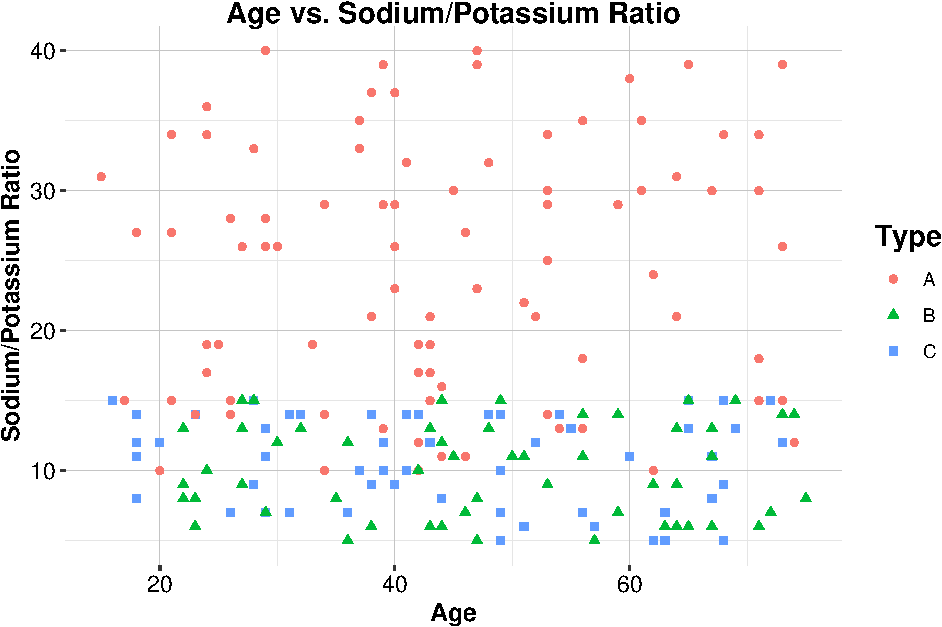
\includegraphics{Intro-R_files/figure-latex/unnamed-chunk-48-1} \end{center}

\begin{enumerate}
\def\labelenumi{\arabic{enumi}.}
\setcounter{enumi}{21}
\tightlist
\item
  Extend the dataset \passthrough{\lstinline!drug\_data!} by adding a new variable named \passthrough{\lstinline!Outcome!}, which is a factor with two levels (\passthrough{\lstinline!"Good"!} and \passthrough{\lstinline!"Bad"!}).

  \begin{itemize}
  \tightlist
  \item
    Patients with \passthrough{\lstinline!Type == "A"!} should have a higher probability of \passthrough{\lstinline!"Good"!} outcomes.\\
  \item
    Patients with \passthrough{\lstinline!Type == "B"!} and \passthrough{\lstinline!Type == "C"!} should have a lower probability of \passthrough{\lstinline!"Good"!} outcomes.\\
  \item
    Use \passthrough{\lstinline!sample()!} with appropriate probabilities to generate the \passthrough{\lstinline!Outcome!} variable.
  \end{itemize}
\end{enumerate}

\chapter{Introduction to Data Science}\label{chapter-intro-DS}

\emph{Data Science} is a rapidly evolving field that is transforming industries by leveraging computational, statistical, and analytical techniques. In the 21st century, data has become one of the most valuable resources, often called the \emph{``new oil''} due to its potential to drive innovation and reshape the future.

Data science is the key to unlocking this potential. By applying computational, statistical, and analytical techniques, data scientists extract insights from vast amounts of data, enabling organizations to make informed decisions, optimize processes, predict trends, and develop intelligent systems. This has led to groundbreaking advancements in fields such as healthcare, finance, marketing, artificial intelligence (AI), and beyond.

Given its rapid growth and increasing demand, data science is more critical than ever. In this chapter, we'll explore the fundamentals of data science, discuss its significance in modern society, and introduce the Data Science Workflow---a structured approach that data scientists use to transform raw data into actionable insights.

This section is well-structured and provides a clear introduction to data science. It effectively conveys the interdisciplinary nature of the field and highlights its core components. However, there are some areas where clarity, consistency, and flow can be improved. Below are my suggestions:

\section{What is Data Science?}\label{what-is-data-science}

Data science is an interdisciplinary field that integrates computer science, statistics, and domain expertise to extract insights from data. It involves using analytical and computational techniques to process vast amounts of raw data, transforming them into meaningful information that supports decision-making and strategic planning.

\begin{figure}

{\centering 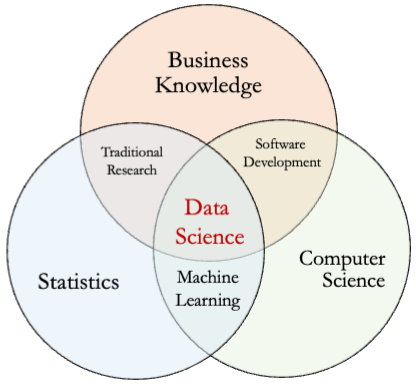
\includegraphics[width=0.5\linewidth]{images/data_science} 

}

\caption{Data science is a multidisciplinary field that applies computational and statistical methods to extract insights from data.}\label{fig:Data-Science}
\end{figure}

Although the term ``data science'' is relatively new, its foundations lie in well-established disciplines such as statistics, data analysis, and machine learning. With the exponential growth of digital data, advancements in computational power, and the increasing demand for data-driven decision-making, data science has emerged as a distinct and essential field.

At its core, data science is concerned with extracting knowledge from data using a combination of statistical techniques, machine learning algorithms, and domain-specific methodologies. It helps organizations manage and understand the vast amounts of information generated in the digital age.

\subsection*{Key Components of Data Science}\label{key-components-of-data-science}
\addcontentsline{toc}{subsection}{Key Components of Data Science}

The field of data science encompasses three main components:

\begin{itemize}
\tightlist
\item
  \textbf{Data Engineering}: The foundation of data science, responsible for collecting, storing, and structuring large datasets. This includes the development of data pipelines and infrastructure to enable efficient analysis. While crucial, data engineering is beyond the scope of this book.\\
\item
  \textbf{Data Analysis and Statistics}: The application of statistical methods to explore and analyze data. This includes data visualization, hypothesis testing, and predictive modeling. More details on this topic are covered in the \hyperref[chapter-statistics]{Statistical Inference and Hypothesis Testing} and \hyperref[chapter-EDA]{Exploratory Data Analysis} chapters.\\
\item
  \textbf{Machine Learning and Artificial Intelligence}: The use of algorithms to identify patterns, make predictions, and extract deeper insights. This includes supervised and unsupervised learning, deep learning, and natural language processing. These concepts are discussed in the \hyperref[chapter-modeling]{Modeling Process} chapter.
\end{itemize}

\section{Why Data Science Matters}\label{why-data-science-matters}

In the digital age, data has become one of the most valuable resources and is often referred to as the ``new oil'' of the 21st century. This comparison makes sense, as some of the world's most valuable companies today---including OpenAI, Google, and Apple---are driven by artificial intelligence and data science. Just as the wealthiest companies of the 20th century were those that controlled oil and energy, today's leading enterprises leverage data as a key asset for innovation and competitive advantage.

Across industries, data-driven decision-making has become essential. Organizations generate vast amounts of data every day, and without the right tools and techniques, much of this data would remain untapped. Data science helps organizations uncover patterns, detect trends, and make informed decisions that enhance efficiency, reduce costs, and improve customer experiences.

Data science plays a crucial role in a wide range of sectors, including:

\begin{itemize}
\tightlist
\item
  \emph{Finance}: Financial institutions leverage data science for risk assessment, fraud detection, and algorithmic trading. Machine learning models identify anomalies in transaction patterns, improving fraud detection and regulatory compliance.\\
\item
  \emph{Marketing}: Businesses use data science to analyze customer behavior, segment audiences, and create targeted marketing campaigns. Platforms such as Facebook and Google Ads leverage sophisticated algorithms to match advertisements with the most relevant audiences, improving engagement and conversion rates.\\
\item
  \emph{Retail and E-commerce}: Companies like Amazon and Walmart use data science to optimize inventory management, predict demand, and personalize recommendations. By analyzing purchase history and browsing behavior, retailers can offer tailored promotions and enhance customer satisfaction.\\
\item
  \emph{Healthcare}: Hospitals and medical researchers use data science for disease diagnosis, patient risk prediction, and personalized treatment plans. By analyzing large datasets of medical records, institutions can identify high-risk patients and take preventative measures to improve health outcomes.
\end{itemize}

For example, Netflix applies data science to analyze viewing patterns and recommend personalized content to users, while supply chain optimization at Amazon ensures faster deliveries by leveraging predictive analytics.

\section{The Data Science Workflow}\label{the-data-science-workflow}

The \emph{data science workflow} follows an \emph{iterative} and \emph{cyclical} approach, where insights gained at each stage inform and refine subsequent steps. Unlike a strictly linear process, data science involves continuous refinement to enhance accuracy and efficiency. This structured approach ensures that data-driven projects are conducted systematically, balancing exploratory analysis, model building, and evaluation to derive meaningful conclusions.

A \emph{data science workflow} follows a phased, adaptive approach within a scientific framework, transforming raw data into actionable knowledge. This transformation is often conceptualized using the \emph{DIKW Pyramid} (Data → Information → Knowledge → Wisdom), as illustrated in Figure \ref{fig:DIKW-Pyramid}.

\begin{figure}

{\centering 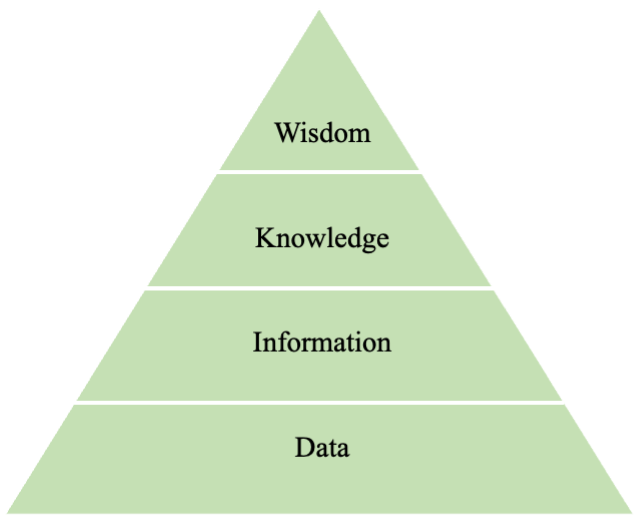
\includegraphics[width=0.4\linewidth]{images/DIKW-Pyramid} 

}

\caption{The DIKW Pyramid illustrates the transformation of raw data into actionable insights, progressing from data to information, knowledge, and ultimately wisdom.}\label{fig:DIKW-Pyramid}
\end{figure}

While the specifics may vary across projects, most data science workflows follow a common structure. In this book, we adopt the \emph{Data Science Workflow} as a guiding framework for structuring data science projects. This workflow is inspired by the \emph{Cross-Industry Standard Process for Data Mining (CRISP-DM)} model, a widely recognized methodology for data-driven projects. It is a \emph{cyclic} framework that guides data scientists through the following key stages (see Figure \ref{fig:CRISP-DM}):

\begin{enumerate}
\def\labelenumi{\arabic{enumi}.}
\tightlist
\item
  \textbf{Problem Understanding} -- Defining the business or research question and outlining objectives.\\
\item
  \textbf{Data Preparation} -- Collecting, cleaning, transforming, and organizing data to ensure it is suitable for analysis. This step includes handling missing values, addressing inconsistencies, detecting outliers, and preparing features through scaling, encoding, and transformation.\\
\item
  \textbf{Exploratory Data Analysis (EDA)} -- Identifying patterns, distributions, and relationships within the data.\\
\item
  \textbf{Preparing Data for Modeling} -- Engineering relevant features, normalizing data, and selecting meaningful variables.\\
\item
  \textbf{Modeling} -- Applying machine learning or statistical techniques to develop predictive or descriptive models.\\
\item
  \textbf{Evaluation} -- Assessing model performance using appropriate metrics and validation techniques.\\
\item
  \textbf{Deployment} -- Integrating the model into a production environment and monitoring its performance over time.
\end{enumerate}

\begin{figure}

{\centering 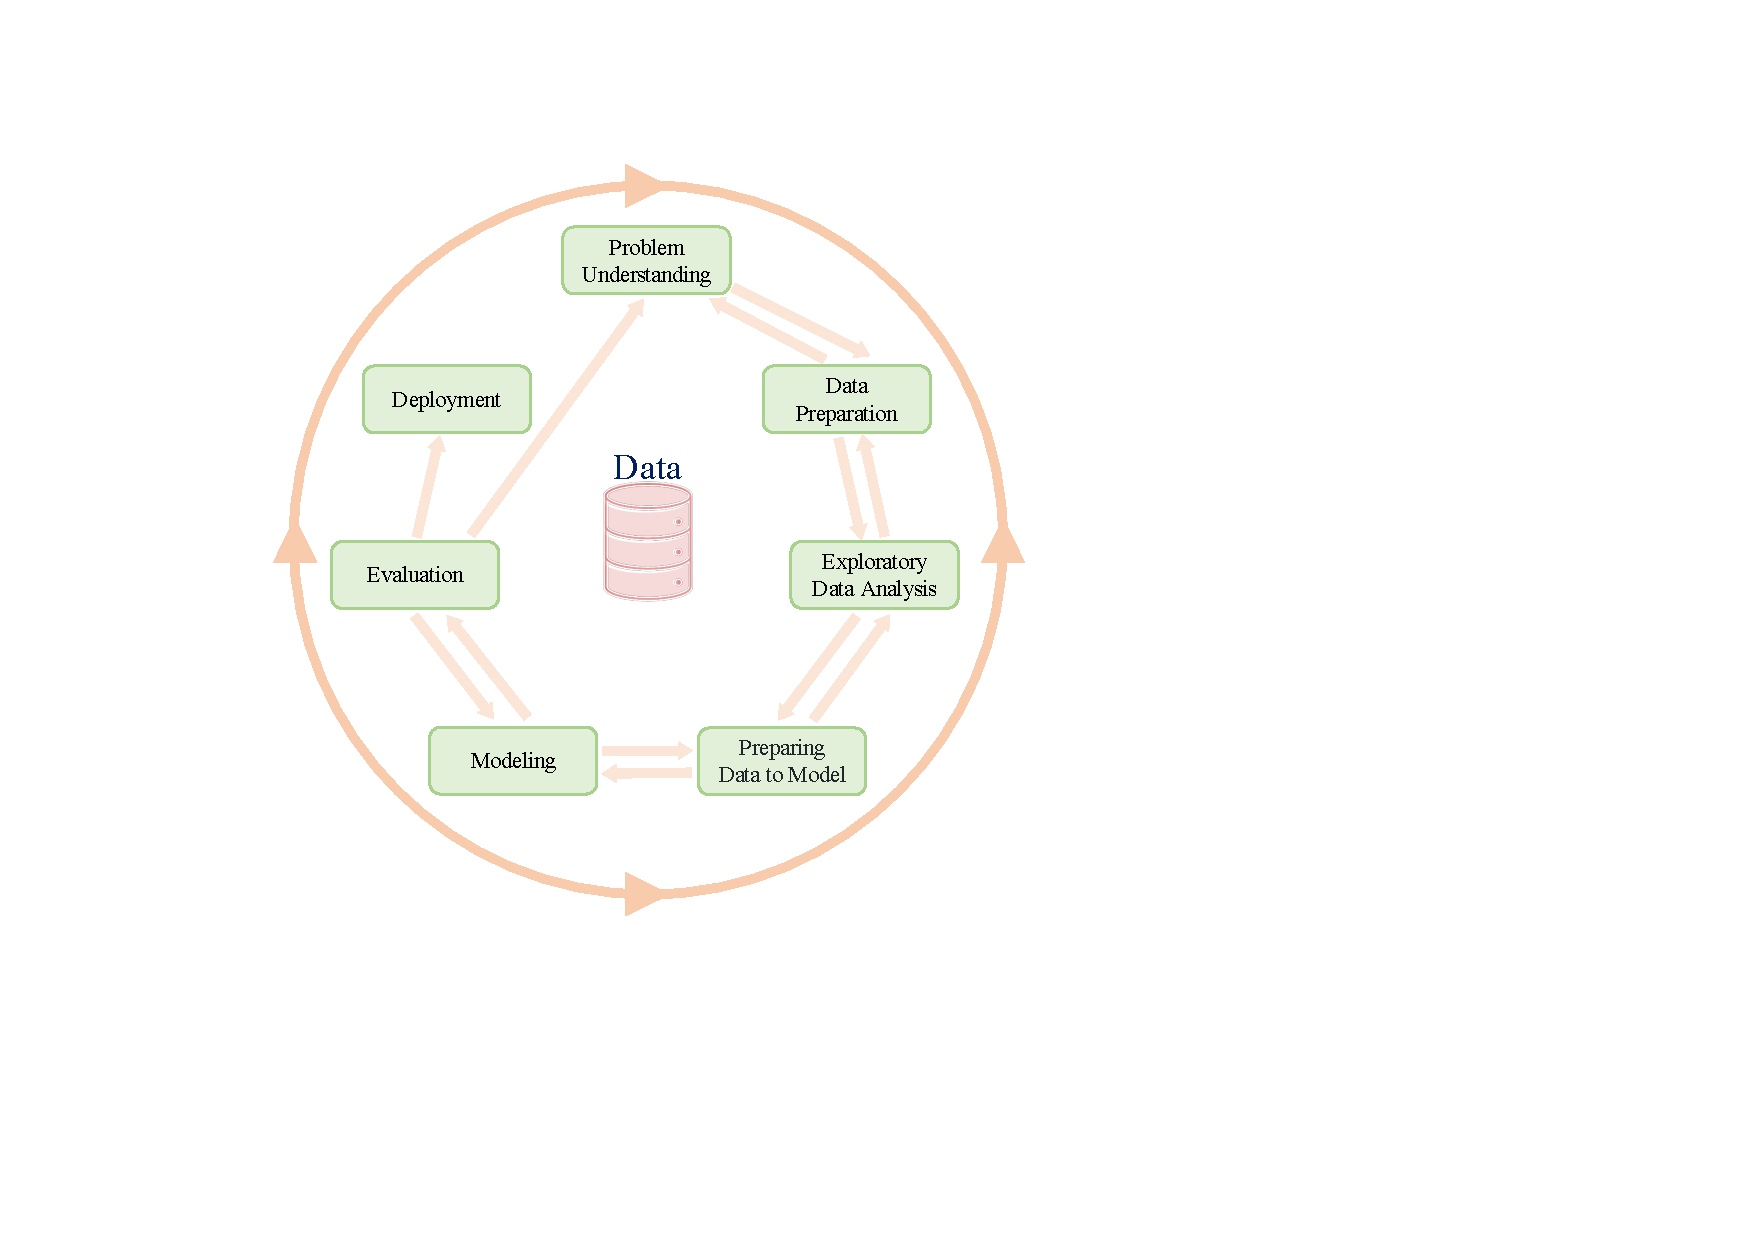
\includegraphics[width=0.6\linewidth]{images/DSW} 

}

\caption{The Data Science Workflow is an iterative framework for structuring data science and machine learning projects. Inspired by the CRISP-DM model, it ensures systematic problem-solving and continuous refinement.}\label{fig:CRISP-DM}
\end{figure}

Because data science is inherently \emph{iterative}, these steps are often revisited multiple times within a single project. The \emph{feedback loops} between stages allow for continuous refinement---adjusting data preprocessing, modifying features, or retraining models as new insights emerge. By following a structured workflow, data scientists can ensure rigor, accuracy, and efficiency in transforming data into valuable insights.

\section{Problem Understanding}\label{problem-understanding}

The first step in any data science project is to clearly define the problem---whether it is a business challenge or a research question. This phase is crucial because data science is not just about building models; it is about solving real-world problems using data-driven approaches. A well-defined problem ensures that efforts are aligned with meaningful objectives, improving the likelihood of delivering actionable insights.

At this stage, data scientists work closely with stakeholders to understand the goals, clarify expectations, and define success criteria. The following questions help frame the problem:

\begin{itemize}
\tightlist
\item
  \textbf{Why} is this research or business question important?\\
\item
  \textbf{What} is the desired outcome or impact?\\
\item
  \textbf{How} can data science techniques contribute to addressing this question?
\end{itemize}

Focusing on the \emph{why} and \emph{what} before diving into the \emph{how} is essential. As Simon Sinek emphasizes in his TED talk \href{https://www.ted.com/talks/simon_sinek_how_great_leaders_inspire_action?utm_campaign=tedspread&utm_medium=referral&utm_source=tedcomshare}{``How Great Leaders Inspire Action''}, ``People don't buy what you do; they buy why you do it.'' This concept applies to data science as well---understanding the deeper motivation behind a project provides clarity and direction.

For example, a data science team in a business analytics department may be approached by a client who wants a predictive model but lacks clarity on the specific problem they are trying to solve. Without a clear \emph{why}, it becomes difficult to develop a solution that delivers real value. Similarly, students working on research projects often focus on \emph{what} they want to build rather than \emph{why} it is needed.

Suppose a company aims to reduce customer churn. A well-defined objective might be to develop a predictive model that identifies customers at risk of leaving so that targeted retention strategies can be implemented. This initial understanding helps frame the problem and guides the selection of relevant data, modeling techniques, and evaluation metrics.

Problem understanding is both an analytical and creative process. While data science provides tools and methodologies, defining the right problem requires domain expertise and critical thinking. The following steps help ensure a structured approach:

\begin{enumerate}
\def\labelenumi{\arabic{enumi}.}
\tightlist
\item
  \textbf{Clearly articulate the project objectives} and requirements in terms of the overall goals of the business or research entity.
\item
  \textbf{Break down the objectives} to outline specific expectations and desired outcomes.
\item
  \textbf{Translate these objectives into a data science problem} that can be addressed using analytical techniques.
\item
  \textbf{Draft a preliminary strategy} for how to achieve these objectives, considering potential approaches and methodologies.
\end{enumerate}

By thoroughly defining the problem, data scientists set the stage for an effective workflow, ensuring that subsequent analysis and modeling efforts remain aligned with meaningful outcomes.

\section{Data Preparation}\label{data-preparation}

Once the problem is well-defined, the next step is \emph{data preparation}, ensuring the data is accurate, complete, and well-structured. Raw data often contains \emph{missing values, inconsistencies, and outliers}, making this phase critical for reliable analysis. Poorly prepared data can lead to misleading insights, even with sophisticated models.

Data can originate from various sources, including databases, spreadsheets, APIs, and web scraping. It may be \emph{structured} (e.g., numerical data in databases) or \emph{unstructured} (e.g., text, images). Preprocessing is essential before analysis.

Key steps in data preparation include:

\begin{itemize}
\tightlist
\item
  \emph{Data Collection and Integration}: Merging data from multiple sources while ensuring consistency.\\
\item
  \emph{Handling Missing Values}: Removing, imputing, or flagging incomplete data.\\
\item
  \emph{Outlier Detection}: Identifying and managing extreme values using visualization.\\
\item
  \emph{Resolving Inconsistencies}: Standardizing formats, correcting errors, and aligning categorical values.\\
\item
  \emph{Feature Engineering}: Transforming data through encoding, scaling, and normalization for model compatibility.\\
\item
  \emph{Data Summarization}: Checking variable types, computing summary statistics, and detecting duplicates.
\end{itemize}

Though time-consuming, data preparation is essential for accurate modeling and meaningful analysis. In Chapter \ref{chapter-data-prep}, we explore these techniques further with real-world examples.

\section{Exploratory Data Analysis (EDA)}\label{exploratory-data-analysis-eda}

Exploratory Data Analysis (EDA) is a fundamental step in the data science workflow, providing an initial understanding of the dataset before formal modeling. The primary objective of EDA is to uncover patterns, relationships, and anomalies in the data, helping data scientists refine hypotheses and validate assumptions. By systematically examining the data, EDA ensures that the subsequent modeling process is informed by a solid understanding of the dataset's structure and characteristics.

Several key techniques are commonly used in EDA:

\begin{itemize}
\tightlist
\item
  \emph{Summary statistics} -- Measures such as the mean, median, standard deviation, and interquartile range provide insights into the distribution and central tendencies of numerical variables.\\
\item
  \emph{Data visualization} -- Graphical techniques, including histograms, scatter plots, and box plots, reveal data distributions, trends, and potential outliers.\\
\item
  \emph{Correlation analysis} -- Examining relationships between numerical features using correlation coefficients helps identify dependencies that may influence modeling decisions.
\end{itemize}

EDA serves both diagnostic and exploratory functions. It helps detect data quality issues, such as missing values or inconsistencies, while also guiding feature selection and engineering. For instance, if a strong correlation exists between certain features and the target variable, these features may be prioritized in the modeling phase.

A thorough EDA process not only improves the quality of the dataset but also enhances the interpretability and reliability of analytical results. In Chapter \ref{chapter-EDA}, we will explore EDA techniques in greater detail, applying them to real-world datasets to illustrate practical applications.

\section{Preparing Data for Modeling}\label{preparing-data-for-modeling}

With insights from EDA, the next step is to \emph{prepare the data for modeling}. This stage involves \emph{feature engineering}, \emph{feature selection}, and \emph{data splitting}---all of which are crucial for building effective models.

\begin{itemize}
\tightlist
\item
  \emph{Feature Engineering}: Creating new features or transforming existing ones to enhance model performance. For example, deriving new variables by combining existing ones or applying transformations can provide additional predictive power.\\
\item
  \emph{Feature Selection}: Identifying and selecting the most relevant features to improve model efficiency and prevent overfitting. Removing irrelevant or redundant features simplifies the model and enhances interpretability.\\
\item
  \emph{Data Splitting}: Dividing the dataset into training, validation, and testing sets. The training set is used to develop the model, the validation set helps fine-tune parameters, and the test set assesses final model performance.
\end{itemize}

By the end of this stage, the data should be in a structured and well-prepared format, ensuring that models can learn effectively. In Chapter \ref{chapter-modeling}, we will explore these techniques in more detail and apply them to real-world datasets.

\section{Modeling}\label{modeling}

Modeling is the stage where data scientists apply machine learning or statistical techniques to the prepared data to create a predictive or descriptive model. The goal is to build a model that effectively captures relationships within the data and generalizes well to new, unseen data.

The modeling process typically involves:

\begin{itemize}
\tightlist
\item
  \emph{Choosing a Model}: Selecting an appropriate model based on the problem type (e.g., regression, classification, clustering) and the characteristics of the dataset.\\
\item
  \emph{Training the Model}: Fitting the model to the training data to learn patterns and relationships.\\
\item
  \emph{Tuning Hyperparameters}: Adjusting model parameters to optimize performance on the validation set.
\end{itemize}

Common algorithms include linear regression (Chapter \ref{chapter-regression}), decision trees (Chapter \ref{chapter-tree}), Naïve Bayes classifier (Chapter \ref{chapter-bayes}), k-Nearest Neighbors (k-NN) algorithm (Chapter \ref{chapter-knn}), and neural networks (Chapter \ref{chapter-nn}). Each method has its strengths and limitations, and selecting the most suitable model depends on the nature of the problem, data quality, and computational constraints. Often, multiple models are tested and compared to determine the best-performing approach.

\section{Evaluation}\label{evaluation}

Once a model is built, it must be rigorously evaluated to ensure its accuracy, generalizability, and robustness before deployment. The evaluation process relies on well-defined performance metrics, which vary depending on the type of problem. For classification models, commonly used metrics include accuracy, precision, recall, F1-score, and the area under the receiver operating characteristic curve (ROC-AUC). In regression tasks, measures such as mean squared error (MSE), mean absolute error (MAE), and the coefficient of determination (\(R^2\)) assess model effectiveness.

To ensure the model is not overfitting to the training data, cross-validation techniques, such as k-fold cross-validation, are employed. These methods provide a more reliable estimate of a model's performance by partitioning the data into multiple subsets for training and validation. Beyond numerical evaluation, error analysis plays a crucial role in diagnosing weaknesses, particularly through confusion matrix interpretation for classification problems and residual analysis for regression. A careful examination of errors often reveals underlying biases, data inconsistencies, or model limitations that require refinement.

If the model fails to meet expectations, adjustments may be necessary, such as feature selection, hyperparameter tuning, or exploring alternative modeling approaches. In Chapter \ref{chapter-evaluation}, we will explore these techniques in detail and apply them to real-world datasets.

\section{Deployment}\label{deployment}

Once the model has been evaluated and meets the project goals, the final step is deployment, where it is integrated into a production environment to generate real-time insights or predictions. This phase is crucial for ensuring that the model contributes tangible value, whether by supporting decision-making processes or by automating tasks within operational systems. Models can be deployed in various ways, such as embedding them in web applications, integrating them into enterprise software, or automating processes in large-scale data pipelines.

Beyond initial integration, continuous monitoring is essential to track the model's performance and detect potential issues. As real-world data evolves, models may experience \emph{concept drift}, where their predictive accuracy deteriorates due to changes in underlying patterns. To mitigate this, periodic model updates and retraining are necessary to maintain reliability. Additionally, implementing robust logging and performance tracking mechanisms helps ensure that discrepancies between predicted and actual outcomes are quickly identified and addressed.

Deployment is not a one-time event but an ongoing process. Effective deployment strategies account for scalability, interpretability, and maintainability, allowing models to remain useful in dynamic environments. As the field of data science advances, the ability to manage deployed models effectively will continue to be a critical factor in transforming analytical insights into real-world impact.

\section{Machine Learning}\label{machine-learning}

Data science relies on machine learning techniques to extract insights from data, make predictions, and uncover patterns. These methods enable data scientists to move beyond descriptive analysis and explore predictive and prescriptive approaches, which are essential for real-world applications. In this section, we provide an overview of machine learning, including its main types---\emph{supervised learning} and \emph{unsupervised learning}---and discuss how machine learning differs from statistical learning.

Machine learning is a branch of artificial intelligence that focuses on developing algorithms that learn from data and make predictions. Rather than being explicitly programmed for each task, machine learning models identify patterns within data and use them to make informed decisions. This approach is particularly useful for complex problems where rule-based programming would be impractical.

For instance, rather than defining a fixed set of rules to detect spam emails, a machine learning model can be trained on a labeled dataset of emails classified as ``spam'' or ``not spam.'' The model learns distinguishing patterns and can classify new emails with high accuracy. This ability to generalize from data makes machine learning invaluable in fields such as finance, healthcare, and marketing.

\subsection*{Machine Learning Tasks: Supervised vs.~Unsupervised Learning}\label{machine-learning-tasks-supervised-vs.-unsupervised-learning}
\addcontentsline{toc}{subsection}{Machine Learning Tasks: Supervised vs.~Unsupervised Learning}

Machine learning tasks can be broadly categorized into \emph{supervised learning} and \emph{unsupervised learning}, which differ in terms of how models learn from data and the objectives of the analysis.

\textbf{Supervised learning} involves training a model on a labeled dataset, where each data point is associated with a known output. The goal is for the model to learn the relationship between input features and the corresponding output, enabling it to make accurate predictions on new data. Common supervised learning tasks include classification and numeric prediction. In classification, the model assigns data points to predefined categories, such as detecting whether an email is spam or identifying whether a patient has a particular disease. This book covers classification techniques such as decision trees (Chapter \ref{chapter-tree}), the Naïve Bayes classifier (Chapter \ref{chapter-bayes}), and the k-Nearest Neighbors (k-NN) algorithm (Chapter \ref{chapter-knn}). Numeric prediction, also known as regression, focuses on estimating continuous values, such as forecasting house prices based on location and size. A detailed discussion of regression techniques is provided in Chapter \ref{chapter-regression}.

\textbf{Unsupervised learning}, on the other hand, is applied to datasets that lack labeled outputs. The objective is to uncover hidden patterns, relationships, or structures within the data. Clustering, a common unsupervised learning technique, groups data points based on similarity, such as segmenting customers according to purchasing behavior. Another important unsupervised learning method is pattern discovery, also known as association rule learning, which identifies relationships between variables. This technique is widely used in market basket analysis to detect frequently co-purchased items. These concepts are explored in further detail in Chapter \ref{chapter-cluster}.

In summary, supervised learning is used when labeled data is available and a specific predictive outcome is required, while unsupervised learning is beneficial for exploratory data analysis, where the goal is to identify underlying structures in unlabeled data. The distinction between these two approaches is fundamental to selecting appropriate machine learning techniques for a given data science problem.

\section{Exercises}\label{exercises-1}

The following exercises will help reinforce the key concepts covered in this chapter. The questions range from fundamental definitions to applied problem-solving related to data science, the data science workflow, and machine learning.

\begin{enumerate}
\def\labelenumi{\arabic{enumi}.}
\item
  Define \emph{data science} and explain its interdisciplinary nature.\\
\item
  Why is data often referred to as the \emph{``new oil''}? Provide examples of industries that benefit from data science.\\
\item
  What are the three key components of data science? Briefly describe their roles.\\
\item
  How does data-driven decision-making impact businesses? Give an example of a real-world application.\\
\item
  Explain the significance of the \emph{DIKW Pyramid} in data science.
\item
  What are the main stages of the data science workflow? Why is it considered an \emph{iterative} process?\\
\item
  Describe the importance of \emph{problem understanding} in a data science project. Provide an example.\\
\item
  Why is \emph{data cleaning} a critical step before analysis? What are some common data quality issues?\\
\item
  How does \emph{exploratory data analysis (EDA)} help in data science? Name two EDA techniques.\\
\item
  Explain the difference between \emph{descriptive analytics}, \emph{predictive analytics}, and \emph{prescriptive analytics}.
\item
  Define \emph{machine learning} and explain how it differs from traditional programming.\\
\item
  What is the key difference between \emph{supervised learning} and \emph{unsupervised learning}? Provide an example of each.\\
\item
  In the context of machine learning, what is a \emph{training dataset} and a \emph{test dataset}? Why are they important?\\
\item
  What is \emph{classification}, and how does it differ from \emph{regression} in supervised learning?\\
\item
  Explain what \emph{clustering} is and provide a real-world scenario where it is useful.
\item
  What is \emph{model evaluation}, and why is it important before deploying a model?\\
\item
  Name and describe two common metrics for evaluating classification models.\\
\item
  What is \emph{cross-validation}, and how does it help assess a model's performance?\\
\item
  Why is \emph{concept drift} a concern in deployed machine learning models? How can it be addressed?\\
\item
  Why is deployment considered an \emph{ongoing process} rather than a one-time step in data science?
\end{enumerate}

\chapter{Data Preparation}\label{chapter-data-prep}

Data preparation is a foundational step in any data science project, ensuring that raw data is transformed into a clean and structured format suitable for analysis. This process is often the most time-consuming yet crucial stage, as the quality of data directly influences the accuracy of insights and the effectiveness of predictive models.

This chapter explores key data preparation techniques, including \emph{handling missing values}, \emph{detecting outliers}, \emph{transforming data}, and \emph{feature engineering}. By the end of this chapter, you will have a clear understanding of how to preprocess raw data, enabling robust statistical modeling and machine learning applications.

To illustrate these concepts, we will use the \emph{diamonds} dataset from the \textbf{ggplot2} package. This dataset contains detailed attributes of diamonds, such as carat, cut, color, clarity, and price, making it an excellent case study for data preprocessing. In this chapter, we focus on the first two steps of the Data Science Workflow---data cleaning and transformation---laying the groundwork for further analysis in subsequent chapters.

\section{Problem Understanding}\label{problem-understanding}

Before preparing data for analysis, it is essential to define the problem and establish clear objectives. In this case, we aim to analyze the \emph{diamonds} dataset to gain insights into \emph{diamond pricing}, a critical factor in industries such as \emph{jewelry retail, gemology, and e-commerce}. The dataset includes attributes that influence diamond value, allowing us to explore the key factors affecting pricing.

\subsection*{Objectives and Key Questions}\label{objectives-and-key-questions}
\addcontentsline{toc}{subsection}{Objectives and Key Questions}

Our primary objectives with the \emph{diamonds} dataset are to:

\begin{enumerate}
\def\labelenumi{\arabic{enumi}.}
\tightlist
\item
  \emph{Examine relationships} between diamond attributes (e.g., carat, cut, color, clarity) and price.\\
\item
  \emph{Identify patterns} that could improve price estimation.\\
\item
  \emph{Assess data quality}, ensuring consistency and detecting missing values or outliers that may affect analysis.
\end{enumerate}

To achieve these objectives, we will address key questions such as:

\begin{itemize}
\tightlist
\item
  Which attributes have the most significant influence on price?\\
\item
  Are there pricing trends based on characteristics such as \emph{carat weight} or \emph{cut quality}?\\
\item
  Are there inconsistencies, errors, or missing values that need to be corrected?
\end{itemize}

\subsection*{Framing the Problem as a Data Science Task}\label{framing-the-problem-as-a-data-science-task}
\addcontentsline{toc}{subsection}{Framing the Problem as a Data Science Task}

From a business perspective, understanding diamond pricing can provide valuable insights for \emph{jewelers, e-commerce platforms, and gemologists}. From a \emph{data science} perspective, this problem can be approached in two ways:

\begin{enumerate}
\def\labelenumi{\arabic{enumi}.}
\tightlist
\item
  \emph{Predictive modeling}: Developing a model that estimates \emph{diamond price} based on its attributes.\\
\item
  \emph{Exploratory data analysis (EDA)}: Identifying trends and relationships without building a predictive model.
\end{enumerate}

Clearly defining these objectives ensures that our data preparation efforts align with the intended analytical approach. This structured problem framing will guide decisions during data cleaning, transformation, and feature engineering, ensuring that our analysis remains focused and actionable.

\section{diamonds Dataset Overview}\label{diamonds-dataset-overview}

The \emph{diamonds} dataset, included in the \textbf{ggplot2} package, provides structured information on various characteristics of diamonds. Each row represents a unique diamond, with 54,940 entries in total, and contains 10 descriptive variables, including \emph{price}, \emph{carat}, \emph{cut}, \emph{clarity}, and \emph{color}. The goal of our analysis is to gain deeper insights into the factors that influence diamond pricing, understand the distribution of data across these attributes, and explore both quantitative and qualitative relationships between variables.

To use the \emph{diamonds} dataset in \textbf{R}, first ensure that the \textbf{ggplot2} package is installed. If not, install it using:

\begin{lstlisting}[language=R]
install.packages("ggplot2") 
\end{lstlisting}

Then, load the package and dataset:

\begin{lstlisting}[language=R]
library(ggplot2)  # Load ggplot2 package
data(diamonds)    # Load diamonds dataset
\end{lstlisting}

To inspect the dataset structure, use:

\begin{lstlisting}[language=R]
str(diamonds)   
   tibble [53,940 x 10] (S3: tbl_df/tbl/data.frame)
    $ carat  : num [1:53940] 0.23 0.21 0.23 0.29 0.31 0.24 0.24 0.26 0.22 0.23 ...
    $ cut    : Ord.factor w/ 5 levels "Fair"<"Good"<..: 5 4 2 4 2 3 3 3 1 3 ...
    $ color  : Ord.factor w/ 7 levels "D"<"E"<"F"<"G"<..: 2 2 2 6 7 7 6 5 2 5 ...
    $ clarity: Ord.factor w/ 8 levels "I1"<"SI2"<"SI1"<..: 2 3 5 4 2 6 7 3 4 5 ...
    $ depth  : num [1:53940] 61.5 59.8 56.9 62.4 63.3 62.8 62.3 61.9 65.1 59.4 ...
    $ table  : num [1:53940] 55 61 65 58 58 57 57 55 61 61 ...
    $ price  : int [1:53940] 326 326 327 334 335 336 336 337 337 338 ...
    $ x      : num [1:53940] 3.95 3.89 4.05 4.2 4.34 3.94 3.95 4.07 3.87 4 ...
    $ y      : num [1:53940] 3.98 3.84 4.07 4.23 4.35 3.96 3.98 4.11 3.78 4.05 ...
    $ z      : num [1:53940] 2.43 2.31 2.31 2.63 2.75 2.48 2.47 2.53 2.49 2.39 ...
\end{lstlisting}

This function reveals that the dataset has 53940 observations and 10 variables. Below is a summary of the key attributes:

\begin{itemize}
\tightlist
\item
  \passthrough{\lstinline!price!}: price in US dollars (\$326--\$18,823).
\item
  \passthrough{\lstinline!carat!}: weight of the diamond (0.2--5.01).
\item
  \passthrough{\lstinline!cut!}: quality of the cut (Fair, Good, Very Good, Premium, Ideal).
\item
  \passthrough{\lstinline!color!}: diamond color, from D (best) to J (worst).
\item
  \passthrough{\lstinline!clarity!}: a measurement of how clear the diamond is (I1 (worst), SI2, SI1, VS2, VS1, VVS2, VVS1, IF (best)).
\item
  \passthrough{\lstinline!x!}: length in mm (0--10.74).
\item
  \passthrough{\lstinline!y!}: width in mm (0--58.9).
\item
  \passthrough{\lstinline!z!}: depth in mm (0--31.8).
\item
  \passthrough{\lstinline!depth!}: total depth percentage = \passthrough{\lstinline!2 * z / (x + y)!}.
\item
  \passthrough{\lstinline!table!}: width of the top of the diamond relative to its widest point.
\end{itemize}

\subsection*{\texorpdfstring{Types of Features in the \texttt{diamonds} Dataset}{Types of Features in the diamonds Dataset}}\label{types-of-features-in-the-diamonds-dataset}
\addcontentsline{toc}{subsection}{Types of Features in the \texttt{diamonds} Dataset}

Understanding the types of features in the dataset is essential for determining the appropriate data preparation steps:

\begin{enumerate}
\def\labelenumi{\arabic{enumi}.}
\tightlist
\item
  \emph{Quantitative (or Numerical) Variables}: These are represented by numbers and can be continuous or discrete.

  \begin{itemize}
  \tightlist
  \item
    \emph{Continuous Variables}: These variables can take any value within a range. In this dataset, \passthrough{\lstinline!carat!}, \passthrough{\lstinline!price!}, \passthrough{\lstinline!x!}, \passthrough{\lstinline!y!}, \passthrough{\lstinline!z!}, and \passthrough{\lstinline!depth!} are continuous.
  \item
    \emph{Discrete Variables}: These variables take countable values, often integers. For example, a count of customers or the number of purchases would be discrete, though this dataset doesn't include such a variable.
  \end{itemize}
\item
  \emph{Categorical (or Qualitative) Variables}: These describe data that fits into categories rather than having a numerical value. They are divided into three types:

  \begin{itemize}
  \tightlist
  \item
    \emph{Ordinal Variables}: Categorical variables with a meaningful order, but where the intervals between categories are not equal. For instance, \passthrough{\lstinline!cut!}, \passthrough{\lstinline!color!}, and \passthrough{\lstinline!clarity!} are ordinal variables in this dataset. The ordering of levels in these variables (e.g., from ``Fair'' to ``Ideal'' in \passthrough{\lstinline!cut!}) has meaning.
  \item
    \emph{Nominal Variables}: Categorical variables without any intrinsic ordering among categories. In other datasets, examples might include ``gender'' or ``product type,'' but the \emph{diamonds} dataset does not contain any nominal variables.
  \item
    \emph{Binary Variables}: Variables with only two levels, often coded as 0 and 1. While the \emph{diamonds} dataset doesn't contain binary variables, an example could be a feature like ``has\_certificate'' with values ``yes'' or ``no.''
  \end{itemize}
\end{enumerate}

Knowing the type of each feature guides decisions about data preparation. For instance:
- \emph{Numerical variables} can be normalized or standardized using techniques like Min-Max Scaling or Z-score Scaling.
- \emph{Ordinal variables} may be encoded using ordinal encoding or one-hot encoding, depending on whether the model should recognize the order.
- \emph{Categorical variables} without a meaningful order are typically one-hot encoded.

By understanding the types of variables in the \emph{diamonds} dataset, we can select appropriate transformations and encoding methods to prepare the data effectively for analysis and modeling.

\subsection*{Key Considerations for Data Preparation}\label{key-considerations-for-data-preparation}
\addcontentsline{toc}{subsection}{Key Considerations for Data Preparation}

With our objectives in mind, here are the main priorities for preparing this dataset:

\begin{itemize}
\tightlist
\item
  \emph{Data Quality}: Ensure that the data is accurate, consistent, and free from major issues. This involves checking for missing values, outliers, and inconsistencies that could bias our analysis.
\item
  \emph{Feature Engineering}: Explore the possibility of creating new features to improve predictive accuracy. For instance, calculating \emph{volume} (using the product of \emph{x}, \emph{y}, and \emph{z} dimensions) could provide an additional measure of a diamond's size.
\item
  \emph{Data Transformation}: Ensure that all features are in appropriate formats. Categorical variables like \emph{cut} and \emph{color} may need to be converted into numeric codes or dummy variables to work with machine learning algorithms effectively.
\end{itemize}

\section{Outliers}\label{outliers}

Outliers are data points that significantly deviate from the general distribution of a dataset. They can arise due to measurement variability, data entry errors, or genuinely unique observations. Identifying and handling outliers is crucial, as they can skew statistical analyses, affect model performance, and lead to misleading insights.

Outliers play a critical role in multiple industries:

\begin{itemize}
\tightlist
\item
  \emph{Finance}: Outliers in transaction data can indicate fraud. Detecting unusually high spending patterns is key to fraud detection models.
\item
  \emph{Healthcare}: Medical records often contain anomalous lab results, which may indicate rare diseases or measurement errors.
\item
  \emph{Manufacturing}: Sensors in factories may detect equipment failures through unusual temperature spikes.
\end{itemize}

In many cases, outliers are not errors but signals of important events. Understanding their role in data analysis ensures that we don't remove valuable insights unintentionally.

\subsection*{Identifying Outliers Using Visualization Techniques}\label{identifying-outliers-using-visualization-techniques}
\addcontentsline{toc}{subsection}{Identifying Outliers Using Visualization Techniques}

\subsubsection*{Boxplots: Detecting Extreme Values}\label{boxplots-detecting-extreme-values}
\addcontentsline{toc}{subsubsection}{Boxplots: Detecting Extreme Values}

Boxplots are a visual tool for detecting extreme values. Below is a boxplot of the \passthrough{\lstinline!y!} variable (diamond width) by using the \textbf{ggplot()} and \passthrough{\lstinline!geom\_boxplot()!} functions from the \textbf{ggplot2} package:

\begin{lstlisting}[language=R]
ggplot(data = diamonds) +
    geom_boxplot(mapping = aes(y = y))
\end{lstlisting}

\begin{center}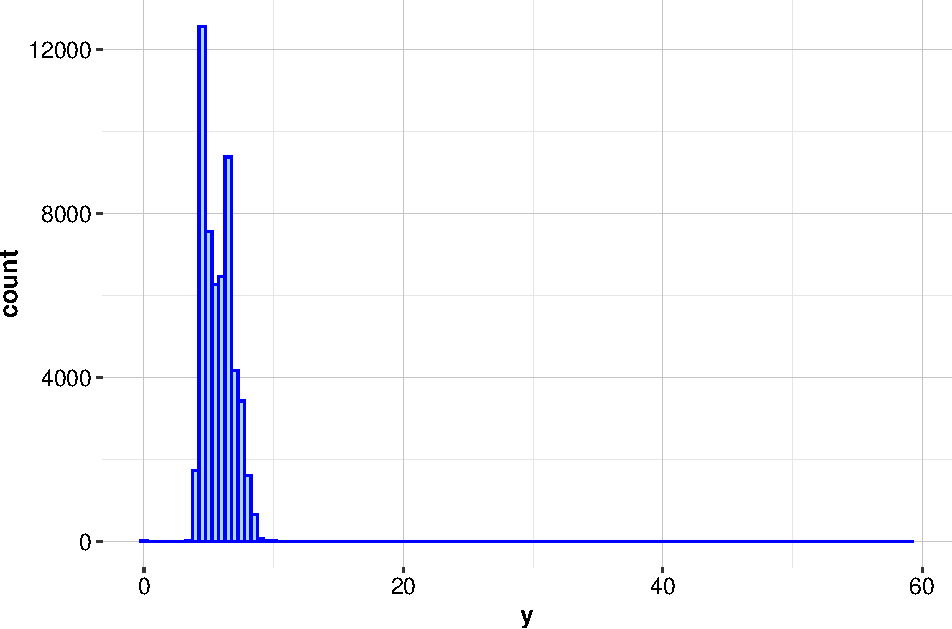
\includegraphics[width=0.7\linewidth]{data-preparation_files/figure-latex/unnamed-chunk-5-1} \end{center}

Here, boxplots highlight values beyond the whiskers, which may indicate potential outliers. Since diamonds cannot have a width of 0 mm, values like 32 mm or 59 mm likely result from data entry errors.

\subsubsection*{Histograms: Understanding Outlier Distribution}\label{histograms-understanding-outlier-distribution}
\addcontentsline{toc}{subsubsection}{Histograms: Understanding Outlier Distribution}

Histograms provide another visual approach to detecting outliers by displaying the frequency distribution of values. Below is a histogram of the \passthrough{\lstinline!y!} variable by using the \emph{ggplot()} and \emph{geom\_histogram()} functions:

\begin{lstlisting}[language=R]
ggplot(data = diamonds) +
    geom_histogram(aes(x = y), binwidth = 0.5, color = 'blue', fill = "lightblue")
\end{lstlisting}

\begin{center}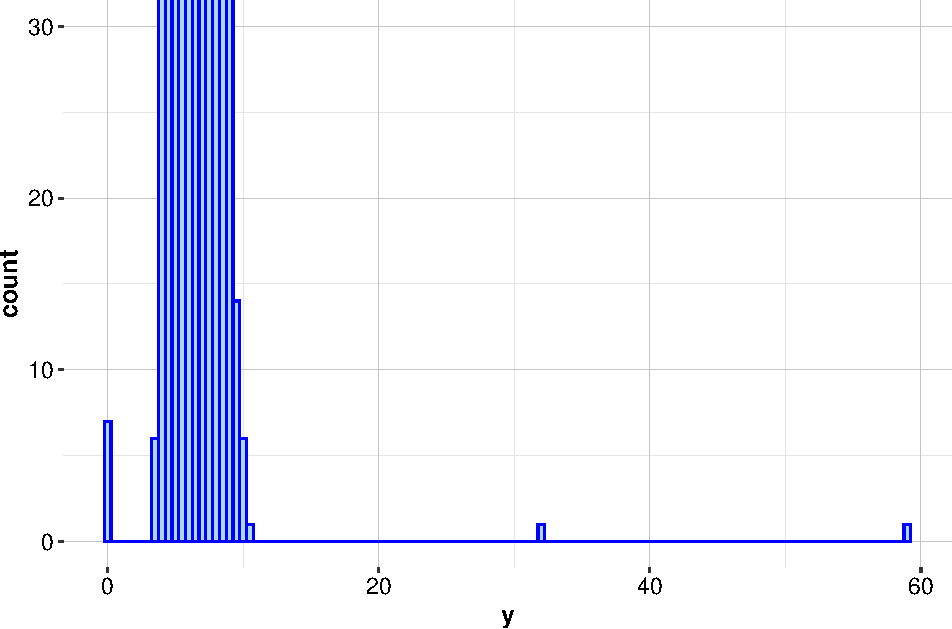
\includegraphics[width=0.7\linewidth]{data-preparation_files/figure-latex/unnamed-chunk-6-1} \end{center}

To enhance visibility, we can zoom in on smaller frequencies by using the \emph{coord\_cartesian()} function from the \textbf{ggplot2} package:

\begin{lstlisting}[language=R]
ggplot(data = diamonds) +
    geom_histogram(mapping = aes(x = y), binwidth = 0.5, color = 'blue', fill = "lightblue") + 
    coord_cartesian(ylim = c(0, 30))
\end{lstlisting}

\begin{center}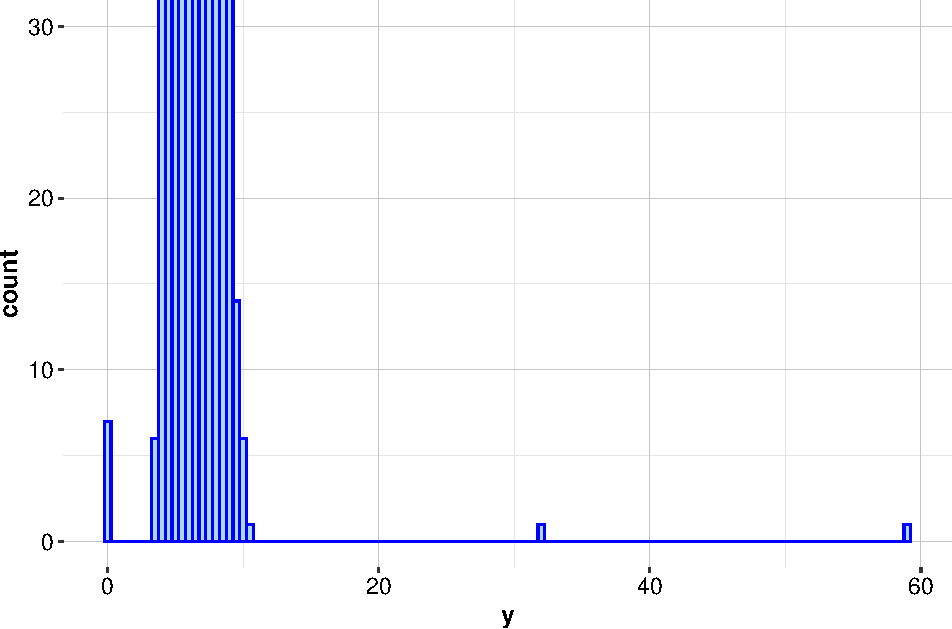
\includegraphics[width=0.7\linewidth]{data-preparation_files/figure-latex/unnamed-chunk-7-1} \end{center}

Other useful visualization techniques include:

\begin{itemize}
\tightlist
\item
  Violin plots -- Show both outliers and density distributions.
\item
  Density plots -- Provide smoother insights into rare values and multimodal distributions.
\end{itemize}

\subsection*{Handling Outliers: Best Practices}\label{handling-outliers-best-practices}
\addcontentsline{toc}{subsection}{Handling Outliers: Best Practices}

Once outliers are identified, there are several strategies for handling them:

\begin{enumerate}
\def\labelenumi{\arabic{enumi}.}
\tightlist
\item
  \emph{Removing outliers}: This is appropriate when an outlier is clearly an error (e.g., negative height, duplicate data entry).
\item
  \emph{Transforming values}: Techniques such as log transformation or square root scaling can reduce the influence of extreme values while preserving trends.
\item
  \emph{Winsorization}: Instead of removing outliers, replace them with the nearest percentile-based value (e.g., capping extreme values at the 95th percentile).
\item
  \emph{Using robust statistical methods}: Some algorithms, like median-based regression or random forests, are less sensitive to outliers.
\item
  \emph{Treating outliers as a separate category}: In fraud detection or rare event prediction, outliers may contain valuable insights and should not be removed.
\end{enumerate}

Choosing the right strategy depends on the context of the analysis and the potential impact of the outlier.

\subsection*{Expanded Code Example: Handling Outliers in R}\label{expanded-code-example-handling-outliers-in-r}
\addcontentsline{toc}{subsection}{Expanded Code Example: Handling Outliers in R}

After detecting outliers, we can choose to either replace them with \passthrough{\lstinline!NA!} values or remove them. For this, we could consider using the \passthrough{\lstinline!mutate()!} function from the \textbf{dplyr} package. Here's an example of treating outliers as missing values using \passthrough{\lstinline!mutate()!} and \passthrough{\lstinline!ifelse()!}:

\begin{lstlisting}[language=R]
diamonds_2 <- mutate(diamonds, y = ifelse(y == 0 | y > 30, NA, y))
\end{lstlisting}

Here's how to verify the update:

\begin{lstlisting}[language=R]
summary(diamonds_2$y)
      Min. 1st Qu.  Median    Mean 3rd Qu.    Max.    NA's 
     3.680   4.720   5.710   5.734   6.540  10.540       9
\end{lstlisting}

This method ensures that outliers do not distort the dataset while allowing for further imputation or analysis.

\section{Missing Values}\label{missing-values}

Missing values pose significant challenges in data analysis, as they can lead to biased results, reduce statistical power, and impact the performance of machine learning models. When handling missing data, we typically consider two approaches:

\begin{enumerate}
\def\labelenumi{\arabic{enumi}.}
\tightlist
\item
  Imputation: Replacing missing values with estimated values to retain data integrity.\\
\item
  Removal: Deleting records with missing values, though this may lead to data loss and potential bias.
\end{enumerate}

\subsection*{Imputation Techniques}\label{imputation-techniques}
\addcontentsline{toc}{subsection}{Imputation Techniques}

There are several strategies for imputing missing values, each with different use cases:

\begin{itemize}
\tightlist
\item
  Mean, median, or mode imputation: Replaces missing values with the mean, median, or mode of the corresponding column.\\
\item
  Random sampling: Fills missing values with random observations drawn from the existing data distribution.\\
\item
  Predictive imputation: Uses machine learning models such as regression or k-nearest neighbors to estimate missing values.\\
\item
  Multiple imputation: Generates several possible values for missing entries and averages the results to reduce uncertainty.\\
  \#\#\# Example: Random Sampling Imputation in R \{-\}
\end{itemize}

To impute missing values in \passthrough{\lstinline!y!} using random sampling, we use the \passthrough{\lstinline!impute()!} function from the \textbf{Hmisc} package:

\begin{lstlisting}[language=R]
diamonds_2$y <- impute(diamonds_2$y, "random")
\end{lstlisting}

The \passthrough{\lstinline!impute()!} function replaces missing values with randomly sampled values from the existing distribution of \passthrough{\lstinline!y!}, maintaining the overall statistical properties of the dataset.

\subsection*{Best Practices}\label{best-practices}
\addcontentsline{toc}{subsection}{Best Practices}

\begin{itemize}
\tightlist
\item
  Use mean or median imputation for numerical variables when the missing values are missing at random (MAR).\\
\item
  Use mode imputation for categorical variables.\\
\item
  Consider predictive models when the dataset is large and missing values are not completely random.\\
\item
  Always assess the proportion of missing data---if too many values are missing, removing the variable may be a better approach than imputation.
\end{itemize}

\section{Feature Scaling}\label{feature-scaling}

Feature scaling, also known as normalization or standardization, is a crucial step in data preprocessing. It adjusts the range and distribution of numerical features so they are on a similar scale. Many machine learning algorithms, especially those based on distance metrics such as k-nearest neighbors, benefit significantly from scaled input features, as this prevents variables with larger ranges from disproportionately influencing the model's outcome.

For instance, in the \emph{diamonds} dataset, the \passthrough{\lstinline!carat!} variable ranges from 0.2 to 5, while \passthrough{\lstinline!price!} ranges from 326 to 18823. Without scaling, variables like \passthrough{\lstinline!price!} with a wider range can dominate the model's predictions, potentially leading to suboptimal results. To address this, we apply feature scaling techniques to bring all numeric variables onto a comparable scale. In this section, we explore two common scaling methods:

\begin{enumerate}
\def\labelenumi{\arabic{enumi}.}
\tightlist
\item
  \emph{Min-Max Scaling}: Also known as min-max normalization or min-max transformation.
\item
  \emph{Z-score Scaling}: Also known as standardization or Z-score normalization.
\end{enumerate}

Feature scaling provides several benefits:

\begin{itemize}
\tightlist
\item
  \emph{Improved Model Performance}: Ensures that features contribute equally to the model, preventing features with larger numerical ranges from dominating learning algorithms.
\item
  \emph{Better Model Convergence}: Particularly useful for gradient-based optimization methods such as logistic regression and neural networks.
\item
  \emph{More Effective Distance-Based Learning}: Algorithms such as k-means clustering and support vector machines rely on distance calculations, making feature scaling essential.
\item
  \emph{Consistent Feature Interpretation}: By standardizing numerical values, models become easier to compare and interpret.
\end{itemize}

However, feature scaling also has some drawbacks:

\begin{itemize}
\tightlist
\item
  \emph{Potential Loss of Information}: In some cases, scaling can obscure meaningful differences between data points.
\item
  \emph{Impact on Outliers}: Min-max scaling, in particular, is sensitive to extreme values, which can distort the scaled representation.
\item
  \emph{Additional Computation}: Scaling adds preprocessing overhead, particularly when working with large datasets.
\item
  \emph{Reduced Interpretability}: The original units of measurement are lost, making it harder to relate scaled values to real-world meanings.
\end{itemize}

Selecting the right scaling method depends on the characteristics of the data and the requirements of the model. In the next sections, we will explore these methods in more detail and apply them to the \emph{diamonds} dataset.

\section{Min-Max Scaling}\label{min-max-scaling}

Min-Max Scaling transforms the values of a feature to a fixed range, typically \([0, 1]\). This transformation ensures that the minimum value of each feature becomes 0 and the maximum value becomes 1. It is especially useful for algorithms that rely on distance metrics, as it equalizes the contributions of all features, making comparisons more balanced.

The formula for Min-Max Scaling is:

\[
x_{\text{scaled}} = \frac{x - x_{\text{min}}}{x_{\text{max}} - x_{\text{min}}},
\]
where \(x\) is the original feature value, \(x_{\text{min}}\) and \(x_{\text{max}}\) are the minimum and maximum values of the feature, and \(x_{\text{scaled}}\) is the scaled value, ranging between 0 and 1.

Min-Max Scaling is particularly useful for models that require bounded input values, such as neural networks and algorithms relying on gradient-based optimization. However, this method is sensitive to outliers, as extreme values significantly affect the scaled distribution.

\begin{example}
\protect\hypertarget{exm:ex-min-max}{}\label{exm:ex-min-max}To demonstrate Min-Max Scaling, we'll apply it to the \passthrough{\lstinline!carat!} variable in the \emph{diamonds} dataset, where \passthrough{\lstinline!carat!} values range from approximately 0.2 to 5. Using the \passthrough{\lstinline!minmax()!} function from the \textbf{liver} package, we can scale \passthrough{\lstinline!carat!} values to fit within the range {[}0, 1{]}.

\begin{lstlisting}[language=R]
ggplot(data = diamonds) +
  geom_histogram(mapping = aes(x = carat), bins = 30,
                 color = 'blue', fill = "lightblue") +
  ggtitle("Histogram for `carat` without scaling") + 
  xlab("Values for variable `carat`")

ggplot(data = diamonds) +
  geom_histogram(mapping = aes(x = minmax(carat)), bins = 30,
                 color = 'blue', fill = "lightblue") +
  ggtitle("Histogram for `carat` with Min-Max Scaling") + 
  xlab("Values for variable `carat`")
\end{lstlisting}

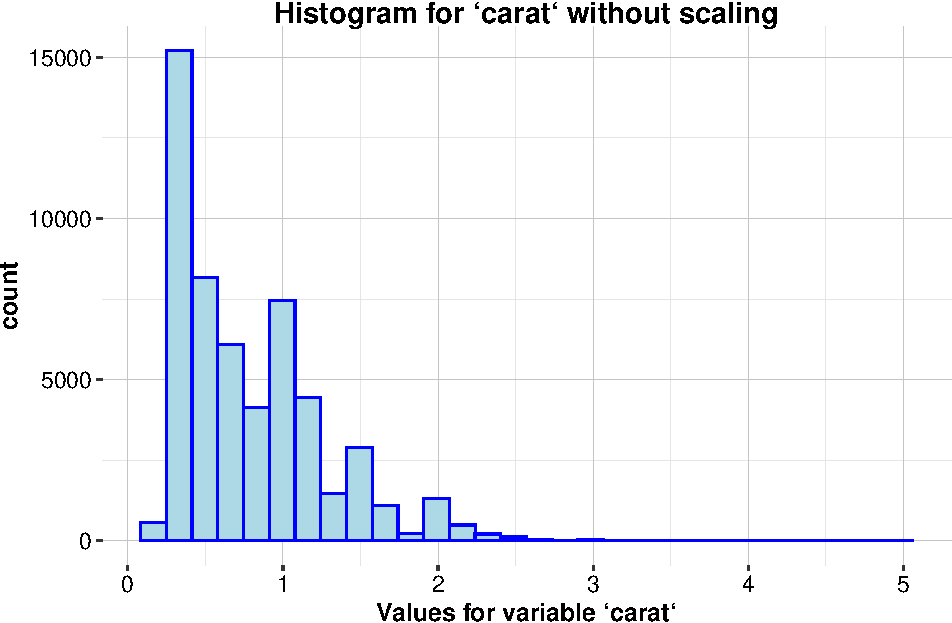
\includegraphics[width=0.5\linewidth]{data-preparation_files/figure-latex/unnamed-chunk-11-1} 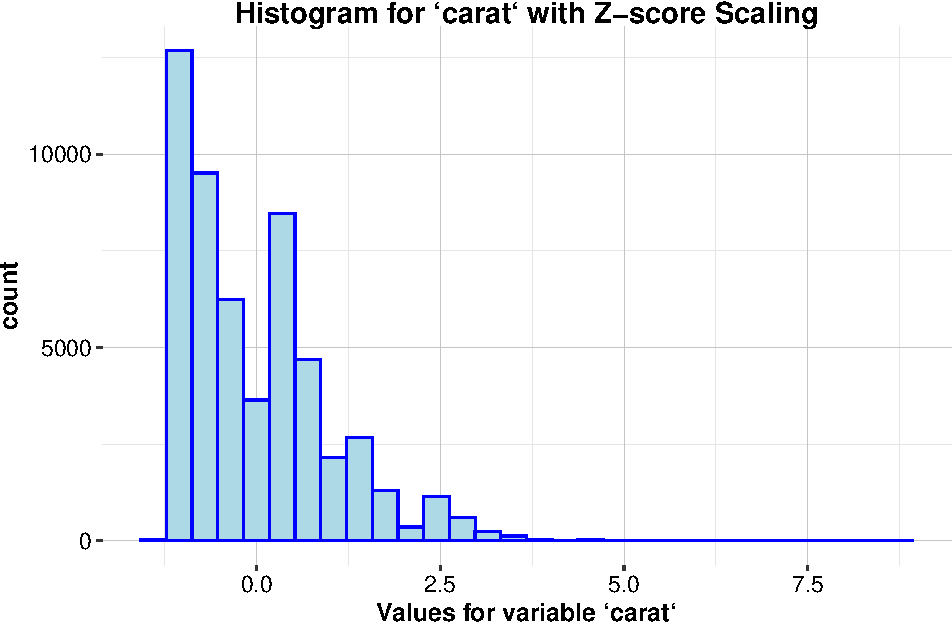
\includegraphics[width=0.5\linewidth]{data-preparation_files/figure-latex/unnamed-chunk-11-2}

The first histogram (left) shows the distribution of \passthrough{\lstinline!carat!} without scaling, while the second histogram (right) shows it after Min-Max Scaling. After scaling, the \passthrough{\lstinline!carat!} values are compressed to a range between 0 and 1, allowing it to be more comparable to other features that may have different original scales. This scaling method is particularly beneficial for distance-based algorithms, as it prevents features with wider ranges from having undue influence.
\end{example}

\section{Z-score Scaling}\label{z-score-scaling}

Z-score Scaling, also known as standardization, transforms feature values so they have a mean of 0 and a standard deviation of 1. This method is particularly useful for algorithms that assume normally distributed data, such as linear regression and logistic regression, because it centers the data around 0 and normalizes the spread of values.

The formula for Z-score Scaling is:

\[
x_{\text{scaled}} = \frac{x - \text{mean}(x)}{\text{sd}(x)}
\]

where \(x\) is the original feature value, \(\text{mean}(x)\) is the mean of the feature, \(\text{sd}(x)\) is the standard deviation of the feature, and \(x_{\text{scaled}}\) is the standardized value, now having a mean of 0 and a standard deviation of 1.

Z-score Scaling is particularly beneficial for models that assume normality or use gradient-based optimization, ensuring that all numerical features contribute equally. However, since it relies on mean and standard deviation, it is \textbf{sensitive to outliers}, which can distort the transformation.

\begin{example}
\protect\hypertarget{exm:ex-zscore}{}\label{exm:ex-zscore}Applying Z-score Scaling to the \passthrough{\lstinline!carat!} variable in the \emph{diamonds} dataset, where the mean and standard deviation of \passthrough{\lstinline!carat!} are approximately 0.8 and 0.47, respectively. We use the \passthrough{\lstinline!zscore()!} function from the \textbf{liver} package to standardize these values.

\begin{lstlisting}[language=R]
ggplot(data = diamonds) +
  geom_histogram(mapping = aes(x = carat), bins = 30,
                 color = 'blue', fill = "lightblue") +
  ggtitle("Histogram for `carat` without scaling") + 
  xlab("Values for variable `carat`")

ggplot(data = diamonds) +
  geom_histogram(mapping = aes(x = zscore(carat)), bins = 30,
                 color = 'blue', fill = "lightblue") +
  ggtitle("Histogram for `carat` with Z-score Scaling") + 
  xlab("Values for variable `carat`")
\end{lstlisting}

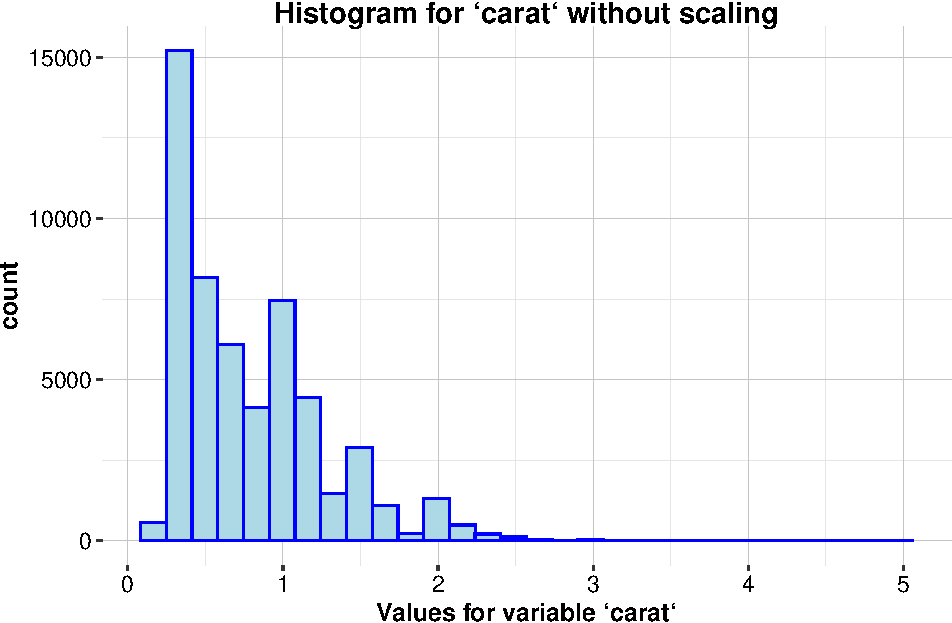
\includegraphics[width=0.5\linewidth]{data-preparation_files/figure-latex/unnamed-chunk-12-1} 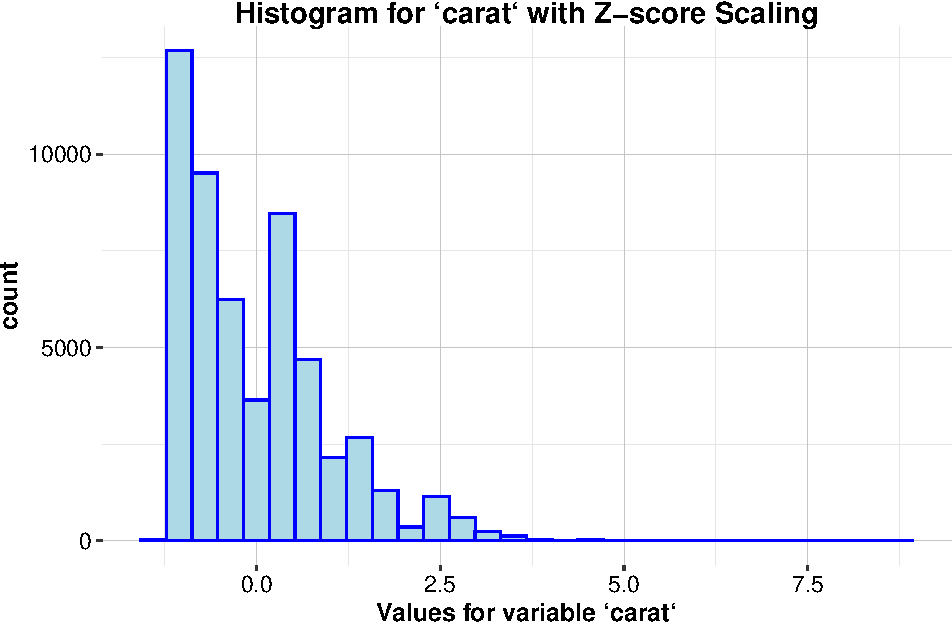
\includegraphics[width=0.5\linewidth]{data-preparation_files/figure-latex/unnamed-chunk-12-2}

The first histogram (left) displays the distribution of \passthrough{\lstinline!carat!} without scaling, while the second histogram (right) shows the distribution after Z-score Scaling. This transformation makes feature values comparable across different scales and ensures that each feature contributes equally to distance-based computations and model training.
\end{example}

\begin{quote}
Note: A common misconception is that after Z-score Scaling, the data follows a standard normal distribution. While Z-score Scaling centers the data to a mean of 0 and scales it to a standard deviation of 1, it does not alter the shape of the distribution. If the original distribution is skewed, it will remain skewed after scaling, as seen in the histograms above.
\end{quote}

The choice between Min-Max Scaling and Z-score Scaling depends on the requirements of the model and the characteristics of the data. Min-Max Scaling is preferable for algorithms that require a fixed input range, while Z-score Scaling is better suited for models that assume normally distributed features. By selecting the appropriate scaling method, we ensure balanced feature contributions and improved model performance.

\section{How to Reexpress Categorical Field Values}\label{how-to-reexpress-categorical-field-values}

In data science, categorical features often need to be transformed into a numeric format before they can be used in machine learning models. Algorithms like decision trees, neural networks, and linear regression require numeric inputs to process the data effectively. Converting categorical variables into numerical representations ensures that all features contribute appropriately to the model, rather than being ignored or treated incorrectly.

This process of reexpressing categorical values is a crucial part of data preparation, as it enables us to leverage the full range of features in our dataset. In this section, we explore several methods to convert categorical fields into numeric representations, with a focus on techniques like one-hot encoding and ordinal encoding. We demonstrate these techniques using the \emph{diamonds} dataset, which includes several categorical features such as \passthrough{\lstinline!cut!}, \passthrough{\lstinline!color!}, and \passthrough{\lstinline!clarity!}.

\subsection{Why Reexpress Categorical Fields?}\label{why-reexpress-categorical-fields}

Categorical fields, also known as nominal or ordinal variables, often represent qualitative aspects of data, such as product types, user locations, or levels of satisfaction. In the \emph{diamonds} dataset, for example:

\begin{itemize}
\tightlist
\item
  \passthrough{\lstinline!cut!} indicates the quality of the diamond's cut (e.g., ``Fair,'' ``Good,'' ``Very Good,'' ``Premium,'' ``Ideal'').
\item
  \passthrough{\lstinline!color!} represents the diamond's color grade (e.g., ``D,'' ``E,'' ``F,'' with ``D'' being the most colorless and thus most valuable).
\item
  \passthrough{\lstinline!clarity!} describes the diamond's clarity, reflecting the absence of internal or external flaws.
\end{itemize}

These fields are essential for understanding and predicting diamond pricing, but in their raw form as text labels, they are not suitable for most machine learning algorithms. Transforming them into numeric form allows us to include these valuable insights in our analysis.

\subsection{Techniques for Reexpressing Categorical Variables}\label{techniques-for-reexpressing-categorical-variables}

There are several approaches to converting categorical variables into numeric representations. The method we choose depends on the type of categorical variable and the nature of the data.

\subsubsection*{Ordinal Encoding}\label{ordinal-encoding}
\addcontentsline{toc}{subsubsection}{Ordinal Encoding}

Ordinal encoding is suitable when the categorical variable has a meaningful order. For example, the \passthrough{\lstinline!cut!} feature in the \emph{diamonds} dataset is ordinal, as there is a natural hierarchy from ``Fair'' to ``Ideal.'' In ordinal encoding, each category is assigned a unique integer based on its rank or level of importance.

In this example, we might assign values as follows:

\begin{itemize}
\tightlist
\item
  ``Fair'' → 1
\item
  ``Good'' → 2
\item
  ``Very Good'' → 3
\item
  ``Premium'' → 4
\item
  ``Ideal'' → 5
\end{itemize}

This approach preserves the order of the categories, which can be useful in models that interpret numeric values in a relative way, such as linear regression. However, it is important to apply ordinal encoding only when the order is meaningful. For non-ordinal variables, other methods like one-hot encoding are more appropriate.

\subsubsection*{One-Hot Encoding}\label{one-hot-encoding}
\addcontentsline{toc}{subsubsection}{One-Hot Encoding}

One-hot encoding is the preferred technique for nominal variables---categorical fields without an intrinsic order. In this approach, each unique category in a field is transformed into a new binary (0 or 1) feature. This method is particularly useful for variables like \passthrough{\lstinline!color!} and \passthrough{\lstinline!clarity!} in the \emph{diamonds} dataset, where the categories do not follow a clear sequence.

For example, if we one-hot encode the \passthrough{\lstinline!color!} feature, we create a set of binary columns, one for each color grade:

\begin{itemize}
\tightlist
\item
  \passthrough{\lstinline!color\_D!}: 1 if the diamond color is ``D,'' 0 otherwise.
\item
  \passthrough{\lstinline!color\_E!}: 1 if the diamond color is ``E,'' 0 otherwise.
\item
  \passthrough{\lstinline!color\_F!}: 1 if the diamond color is ``F,'' 0 otherwise.
\end{itemize}

One-hot encoding avoids introducing false ordinal relationships, ensuring that the model treats each category as an independent entity. However, one downside is that it can significantly increase the dimensionality of the dataset if the categorical field has many unique values.

\begin{quote}
Note: Many machine learning libraries automatically drop one of the binary columns to avoid multicollinearity (perfect correlation among features). For instance, if we have seven color categories, only six binary columns are created, and the missing category is implied when all columns are zero. This approach, known as dummy encoding, helps avoid redundancy and keeps the model simpler.
\end{quote}

\subsubsection*{Frequency Encoding}\label{frequency-encoding}
\addcontentsline{toc}{subsubsection}{Frequency Encoding}

Another useful approach, especially for high-cardinality categorical variables (those with many unique values), is frequency encoding. This technique replaces each category with its frequency in the dataset, allowing the model to capture information about how common each category is. Frequency encoding can be particularly helpful for fields like \passthrough{\lstinline!clarity!} if you want to give the model an indication of how prevalent each level is.

For example:

\begin{itemize}
\tightlist
\item
  If ``VS2'' appears 10,000 times in the dataset, it would be encoded as 10,000.
\item
  If ``IF'' appears only 500 times, it would be encoded as 500.
\end{itemize}

Frequency encoding is less commonly used in basic machine learning workflows but can be valuable when dealing with very large datasets, or when one-hot encoding would introduce too many columns. However, be cautious with this approach, as it may inadvertently add an implicit weight to more common categories.

\subsection{Choosing the Right Encoding Technique}\label{choosing-the-right-encoding-technique}

Selecting the appropriate encoding technique depends on the nature of your categorical variable and the requirements of your analysis:

\begin{itemize}
\tightlist
\item
  Ordinal variables (like \passthrough{\lstinline!cut!}): Use ordinal encoding to preserve the natural order.
\item
  Nominal variables with few unique values (like \passthrough{\lstinline!color!} and \passthrough{\lstinline!clarity!}): Use one-hot encoding to represent each category as a binary column.
\item
  High-cardinality categorical variables: Consider frequency encoding if one-hot encoding would introduce too many features.
\end{itemize}

\begin{example}
\protect\hypertarget{exm:ex-encoding}{}\label{exm:ex-encoding}

Applying these techniques to the \emph{diamonds} dataset:

\begin{lstlisting}[language=R]
# Example: Ordinal encoding for `cut`
diamonds <- diamonds %>%
  mutate(cut_encoded = as.integer(factor(cut, levels = c("Fair", "Good", "Very Good", "Premium", "Ideal"))))

# Example: One-hot encoding for `color`
diamonds <- diamonds %>%
  mutate(
    color_D = ifelse(color == "D", 1, 0),
    color_E = ifelse(color == "E", 1, 0),
    color_F = ifelse(color == "F", 1, 0),
    color_G = ifelse(color == "G", 1, 0),
    color_H = ifelse(color == "H", 1, 0),
    color_I = ifelse(color == "I", 1, 0),
    color_J = ifelse(color == "J", 1, 0)
  )
\end{lstlisting}

In this example:

\begin{itemize}
\tightlist
\item
  Ordinal Encoding: We have encoded the \passthrough{\lstinline!cut!} variable based on its quality hierarchy.
\item
  One-Hot Encoding: We have applied one-hot encoding to \passthrough{\lstinline!color!}, creating binary columns for each color grade.
\end{itemize}

\end{example}

By encoding the categorical fields in this way, we transform the dataset into a format compatible with most machine learning algorithms while preserving the essential information about each categorical feature.

With our dataset now cleaned, scaled, and encoded, we are ready to move into the next stage of data analysis. In the upcoming chapter, we will explore Exploratory Data Analysis (EDA), where we will use visualizations and summary statistics to gain insights into the structure and relationships within the data. By combining the prepared data with EDA techniques, we can better understand which features may hold predictive value for our model and set the stage for successful machine learning outcomes.

\section{Exercises}\label{exercises-2}

To reinforce your understanding of data preparation concepts, answer the following questions:

\begin{enumerate}
\def\labelenumi{\arabic{enumi}.}
\tightlist
\item
  What is the primary goal of data preparation in a data science workflow?
\item
  Why is it important to understand the problem context before preparing data?
\item
  What are the key attributes in the \emph{diamonds} dataset, and why are they relevant for analysis?
\item
  How can we inspect the structure of a dataset in \textbf{R}?
\item
  What is the difference between continuous and discrete numerical variables?
\item
  How do ordinal categorical variables differ from nominal categorical variables?
\item
  Why is handling missing values crucial in data analysis?
\item
  What are two common strategies for dealing with missing values?
\item
  How does the \passthrough{\lstinline!impute()!} function from \textbf{Hmisc} help in handling missing values?
\item
  What are outliers, and how can they impact a dataset?
\item
  How can we detect outliers using a boxplot for the \passthrough{\lstinline!y!} variable in \textbf{ggplot2}?
\item
  How can we detect outliers using a boxplot for the \passthrough{\lstinline!z!} variable in \textbf{ggplot2}?
\item
  How can we detect outliers using a histogram for the \passthrough{\lstinline!x!} variable in \textbf{ggplot2}?
\item
  What are some alternative visualization methods for identifying outliers?
\item
  Why is it sometimes necessary to transform outliers rather than remove them?
\item
  What are the advantages and disadvantages of Min-Max Scaling?
\item
  When should Min-Max Scaling be preferred over Z-score Scaling?
\item
  What is the main purpose of Z-score Scaling, and how does it work?
\item
  How does the presence of outliers impact Z-score Scaling?
\item
  Which machine learning models are most sensitive to unscaled features?
\item
  What are the differences between one-hot encoding and ordinal encoding?
\item
  When is it appropriate to use frequency encoding for categorical variables?
\item
  How does one-hot encoding increase the dimensionality of a dataset?
\item
  How can we encode the \passthrough{\lstinline!cut!} variable in the \emph{diamonds} dataset using ordinal encoding?
\item
  How can we encode the \passthrough{\lstinline!color!} variable in the \emph{diamonds} dataset using one-hot encoding?
\end{enumerate}

\chapter{Exploratory Data Analysis}\label{chapter-EDA}

\textbf{Exploratory Data Analysis (EDA)} is the process of examining and exploring data to gain insights, identify patterns, and understand relationships between variables---all before applying formal hypotheses or machine learning algorithms. This critical step allows us to ``get to know'' the data, using a mix of summary statistics, visualizations, and preliminary analysis to reveal structure and potential insights. EDA is foundational to data science because it helps generate hypotheses and informs the decisions we'll make in later stages of analysis.

EDA is not a rigid process with strict rules; rather, it is a flexible, iterative approach that encourages curiosity and open-ended exploration. At this stage, it's important to remain open to investigating any ideas that arise. Some explorations may lead to dead ends, but others can uncover valuable insights that guide the rest of the project. Over time, as you become more familiar with the data, you'll naturally focus on the most promising leads, which will help shape your final analysis and conclusions.

EDA is primarily about exploration and discovery---it's a way to find clues and patterns in the data rather than proving any particular theory. Using tools like summary statistics, visualizations, and basic correlations, we can generate hypotheses and start to understand the underlying structure of the data. However, these insights are just preliminary observations, not formal conclusions; they provide direction for further analysis, where more rigorous testing can confirm or refine what we uncover during EDA.

When interpreting patterns in EDA, it's essential to balance statistical significance with practical relevance. In large datasets, even small correlations or patterns may be statistically significant, but they might not have meaningful implications for the problem at hand. For example, a variable might show a slight but statistically significant association with churn; however, if this association is weak, it may not be actionable in a real-world context. EDA encourages us to consider both perspectives: while statistical tests can highlight interesting relationships, we also need to interpret these findings in a way that aligns with practical goals and domain knowledge.

EDA also overlaps significantly with data preparation and cleaning. For example, you may notice missing values during EDA and decide to address them by imputing or removing data points. While this is technically part of data cleaning, it's also an aspect of exploration, as we examine the data to make the best decision for handling these issues. Identifying these issues early on allows us to refine the data and set a strong foundation for analysis.

EDA involves choosing the appropriate tools and techniques to answer each question we pose about the data. The choice of visualization or statistical summary depends on the type of data and the specific aspect of the data we're examining. For example, histograms and box plots are helpful for understanding distributions of individual variables, while scatter plots and correlation matrices are better for exploring relationships between pairs of variables. In the following sections, we'll see examples of visualizations and summaries that help answer different types of questions within EDA. We'll also apply these techniques to our churn dataset, which will help illustrate how to use EDA to uncover patterns relevant to customer retention.

\section{Key Areas of Focus in EDA}\label{key-areas-of-focus-in-eda}

During EDA, our primary goals are to:

\begin{enumerate}
\def\labelenumi{\arabic{enumi}.}
\tightlist
\item
  \textbf{Understand the structure of the data}: Determine the data types, range, and number of observations, and identify any missing values or anomalies.
\item
  \textbf{Analyze individual variable distributions}: Explore each variable to understand its distribution, central tendency, and spread.
\item
  \textbf{Explore relationships between variables}: Identify correlations, dependencies, or interactions that may exist between features.
\item
  \textbf{Identify patterns and outliers}: Spot unusual data points and decide whether they require special handling or removal.
\end{enumerate}

These objectives serve as a guide to ensure that we gain a comprehensive understanding of the dataset before moving on to modeling.

\section{Types of EDA Questions}\label{types-of-eda-questions}

When performing EDA, it's helpful to approach the data with specific questions in mind. These questions typically fall into two broad categories: \textbf{univariate questions} and \textbf{multivariate questions}.

\begin{enumerate}
\def\labelenumi{\arabic{enumi}.}
\tightlist
\item
  \textbf{Univariate Questions}: These questions focus on understanding the distribution of individual variables. Examples include:
\end{enumerate}

\begin{itemize}
\tightlist
\item
  What is the distribution of the target variable?
\item
  How are predictor variables like \textbf{age}, \textbf{income}, or \textbf{education} distributed?
\item
  Are there any missing values, and how are they distributed across variables?
\end{itemize}

Answering univariate questions helps you understand each variable in isolation, which is essential for detecting skewness, outliers, and data ranges. You can use \textbf{histograms}, \textbf{box plots}, and \textbf{summary statistics} to explore these characteristics.

\begin{enumerate}
\def\labelenumi{\arabic{enumi}.}
\setcounter{enumi}{1}
\tightlist
\item
  \textbf{Multivariate Questions}: These questions examine the relationships between multiple variables. Examples include:
\end{enumerate}

\begin{itemize}
\tightlist
\item
  What is the relationship between the target variable and predictors?
\item
  Are certain predictors correlated with each other, indicating potential multicollinearity?
\item
  Is there any relationship between missing values in different variables?
\end{itemize}

To answer multivariate questions, use \textbf{scatter plots}, \textbf{correlation matrices}, and \textbf{pair plots} to visualize relationships. These tools reveal interactions between features and can help you detect patterns that could be important for building predictive models.

These questions guide the exploratory process and allow you to uncover insights that will inform later analysis. Keep in mind that EDA is primarily about exploration---finding clues rather than proving theories.

Note that to answer to these types of questions we can use different types of visualizations and statistical summaries. But \emph{how to we know which visualization to use?} This is a question that I hear a lot from my students and the answer it: \emph{It depends on the type of data you have and the question you want to answer}. To be more specific, in the following sections we will see some examples of visualizations and statistical summaries that can be used to answer univariate and multi-variate questions. And we will also see how to use them in practice with the churn dataset. And at the end of this chapter we have a guide line to specificity answer this question.

\section{EDA as Data Storytelling}\label{eda-as-data-storytelling}

EDA is not only a technical exercise but also a form of \textbf{data storytelling}. Data storytelling combines data, visuals, and narrative to communicate insights in a structured, compelling way. This skill is invaluable in data science, as it enables you to present complex findings to audiences in an accessible manner.

Many scientific reports, journalistic pieces, and public presentations rely on data storytelling to convey insights effectively. Figures like the ones below demonstrate how data visualization can bring a narrative to life:

\begin{itemize}
\tightlist
\item
  \textbf{Figure \ref{fig:EDA-fig-1}} illustrates global mean surface temperature changes over the Common Era, using visual cues to communicate a story about temperature anomalies over time. This visualization, taken from \citet{neukom2019consistent}, shows how data can be transformed into a compelling visual narrative.
\end{itemize}

\begin{figure}

{\centering 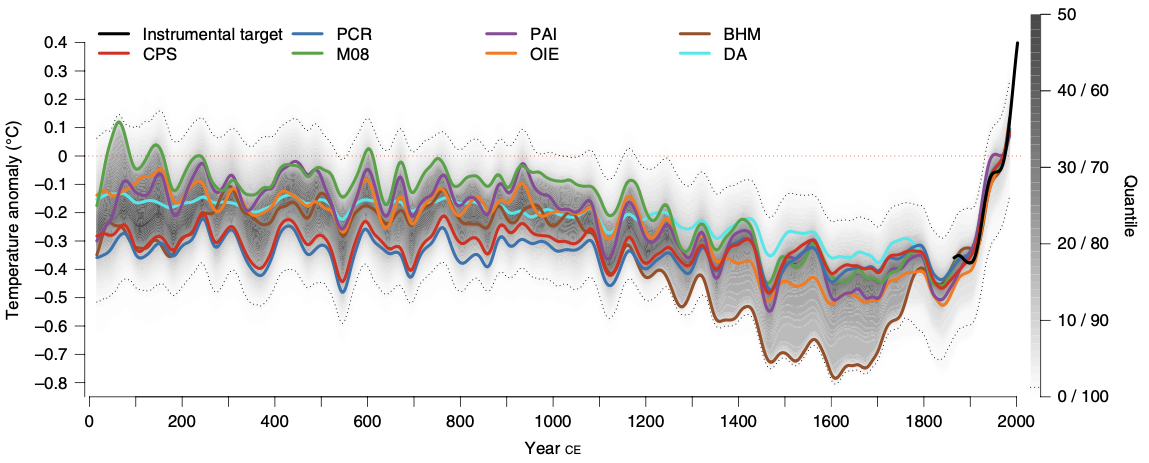
\includegraphics[width=1\linewidth]{images/EDA_fig_1} 

}

\caption{Global mean surface temperature history over the Common Era. Temperature anomalies with respect to 1961–1990 CE. The coloured lines represent 30-year low-pass-filtered ensemble medians for the individual reconstruction methods.}\label{fig:EDA-fig-1}
\end{figure}

\begin{itemize}
\tightlist
\item
  \textbf{Figure \ref{fig:EDA-fig-2}} shows an animated scatter plot of fertility rate versus life expectancy at birth for different world regions between 1960 and 2015. Adapted from Hans Rosling's TED Talk \href{https://www.ted.com/talks/hans_rosling_new_insights_on_poverty?subtitle=en}{``New insights on poverty''}, this visualization effectively illustrates trends in global health and demography through dynamic, multi-dimensional storytelling.
\end{itemize}

\begin{figure}

{\centering 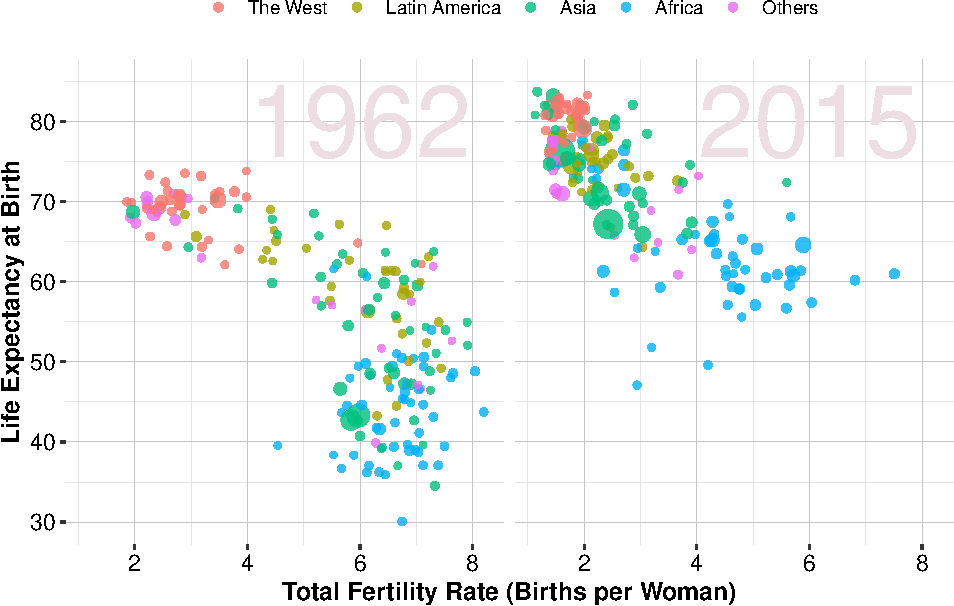
\includegraphics[width=0.8\linewidth]{EDA_files/figure-latex/EDA-fig-2-1} 

}

\caption{Animated scatter plot of fertility rate and life expectancy at birth for different regions of the world from 1960 to 2015.}\label{fig:EDA-fig-2}
\end{figure}

By learning to interpret and create such visualizations, you'll be better equipped to uncover key insights and communicate your findings persuasively.

\section{\texorpdfstring{EDA in Practice: Working with the \emph{Churn} Dataset}{EDA in Practice: Working with the Churn Dataset}}\label{eda-in-practice-working-with-the-churn-dataset}

In this book, we will use the \textbf{churn} dataset to illustrate the EDA process. The churn dataset contains information on customer behavior, including whether a customer has ``churned'' (i.e., left the service) and various demographic and behavioral attributes.

Through EDA, we aim to:

\begin{enumerate}
\def\labelenumi{\arabic{enumi}.}
\tightlist
\item
  Uncover patterns related to customer churn.
\item
  Identify important predictors that influence customer retention.
\item
  Gain insights into the structure of the data that will guide us in building predictive models.
\end{enumerate}

In the next sections, we'll walk through specific techniques for exploring the churn dataset, from calculating summary statistics to creating visualizations. By following these steps, you'll be able to turn raw data into actionable insights, building a strong foundation for further analysis and modeling. But before we shortly the frist and second steps of Data Science workflow.

\subsection{Problem/Business Understanding}\label{problembusiness-understanding}

Companies are interested to know who is gonna get churned so they can proactively go to the customer to provide them better services and turn customers' decisions in the opposite direction. Companies are interested to know:

\begin{itemize}
\tightlist
\item
  \textbf{Why} are we losing them?
\item
  \textbf{What} are the causes or reasons of losing customers?
\item
  \textbf{How} do we stop them from leaving the company?
\end{itemize}

EDA will help us to answer these questions and provide insights to the company to take actions.

\subsection{Data Understanding}\label{data-understanding}

This dataset comes from IBM Sample Data Sets. The data set contains 5000 rows (customers) and 20 columns (features). The ``churn'' column is our target which indicates whether the customer churned (left the company) or not.
The 20 variables are:

\begin{quote}
\begin{enumerate}
\def\labelenumi{\arabic{enumi}.}
\tightlist
\item
  \passthrough{\lstinline!state!}: Categorical, for the 51 states and the District of Columbia.
\item
  \passthrough{\lstinline!area.code!}: Categorical.
\item
  \passthrough{\lstinline!account.length!}: count, how long account has been active.
\item
  \passthrough{\lstinline!voice.plan!}: Categorical, yes or no, voice mail plan.
\item
  \passthrough{\lstinline!voice.messages!}: Count, number of voice mail messages.
\item
  \passthrough{\lstinline!intl.plan!}: Categorical, yes or no, international plan.
\item
  \passthrough{\lstinline!intl.mins!}: Continuous, minutes customer used service to make international calls.
\item
  \passthrough{\lstinline!intl.calls!}: Count, total number of international calls.
\item
  \passthrough{\lstinline!intl.charge!}: Continuous, total international charge.
\item
  \passthrough{\lstinline!day.mins!}: Continuous, minutes customer used service during the day.
\item
  \passthrough{\lstinline!day.calls!}: Count, total number of calls during the day.
\item
  \passthrough{\lstinline!day.charge!}: Continuous, total charge during the day.
\item
  \passthrough{\lstinline!eve.mins!}: Continuous, minutes customer used service during the evening.
\item
  \passthrough{\lstinline!eve.calls!}: Count, total number of calls during the evening.
\item
  \passthrough{\lstinline!eve.charge!}: Continuous, total charge during the evening.
\item
  \passthrough{\lstinline!night.mins!}: Continuous, minutes customer used service during the night.
\item
  \passthrough{\lstinline!night.calls!}: Count, total number of calls during the night.
\item
  \passthrough{\lstinline!night.charge!}: Continuous, total charge during the night.
\item
  \passthrough{\lstinline!customer.calls!}: Count, number of calls to customer service.
\item
  \passthrough{\lstinline!churn!}: Categorical, yes or no. Indicator of whether the customer has left the company (yes or no).
\end{enumerate}
\end{quote}

We import the dataset in \textbf{R} as follows:

\begin{lstlisting}[language=R]
library(liver)

data(churn) # load the "churn" dataset
\end{lstlisting}

To see the overview of the dataset in \textbf{R} we are using function \passthrough{\lstinline!str()!} as follows:

\begin{lstlisting}[language=R]
str(churn)   # Compactly display the structure of the data
   'data.frame':    5000 obs. of  20 variables:
    $ state         : Factor w/ 51 levels "AK","AL","AR",..: 17 36 32 36 37 2 20 25 19 50 ...
    $ area.code     : Factor w/ 3 levels "area_code_408",..: 2 2 2 1 2 3 3 2 1 2 ...
    $ account.length: int  128 107 137 84 75 118 121 147 117 141 ...
    $ voice.plan    : Factor w/ 2 levels "yes","no": 1 1 2 2 2 2 1 2 2 1 ...
    $ voice.messages: int  25 26 0 0 0 0 24 0 0 37 ...
    $ intl.plan     : Factor w/ 2 levels "yes","no": 2 2 2 1 1 1 2 1 2 1 ...
    $ intl.mins     : num  10 13.7 12.2 6.6 10.1 6.3 7.5 7.1 8.7 11.2 ...
    $ intl.calls    : int  3 3 5 7 3 6 7 6 4 5 ...
    $ intl.charge   : num  2.7 3.7 3.29 1.78 2.73 1.7 2.03 1.92 2.35 3.02 ...
    $ day.mins      : num  265 162 243 299 167 ...
    $ day.calls     : int  110 123 114 71 113 98 88 79 97 84 ...
    $ day.charge    : num  45.1 27.5 41.4 50.9 28.3 ...
    $ eve.mins      : num  197.4 195.5 121.2 61.9 148.3 ...
    $ eve.calls     : int  99 103 110 88 122 101 108 94 80 111 ...
    $ eve.charge    : num  16.78 16.62 10.3 5.26 12.61 ...
    $ night.mins    : num  245 254 163 197 187 ...
    $ night.calls   : int  91 103 104 89 121 118 118 96 90 97 ...
    $ night.charge  : num  11.01 11.45 7.32 8.86 8.41 ...
    $ customer.calls: int  1 1 0 2 3 0 3 0 1 0 ...
    $ churn         : Factor w/ 2 levels "yes","no": 2 2 2 2 2 2 2 2 2 2 ...
\end{lstlisting}

It shows that data are as a \emph{data.frame} object in \textbf{R} with 5000 observations and 20 variables. The last column (with name \emph{churn}) is the \emph{target variable} that indicates whether customers churned (left the company) or not.

By using the function \passthrough{\lstinline!summary()!} in \textbf{R}, we can see the summary of the dataset as follows

\begin{lstlisting}[language=R]
summary(churn)
        state              area.code    account.length  voice.plan
    WV     : 158   area_code_408:1259   Min.   :  1.0   yes:1323  
    MN     : 125   area_code_415:2495   1st Qu.: 73.0   no :3677  
    AL     : 124   area_code_510:1246   Median :100.0             
    ID     : 119                        Mean   :100.3             
    VA     : 118                        3rd Qu.:127.0             
    OH     : 116                        Max.   :243.0             
    (Other):4240                                                  
    voice.messages   intl.plan    intl.mins       intl.calls      intl.charge   
    Min.   : 0.000   yes: 473   Min.   : 0.00   Min.   : 0.000   Min.   :0.000  
    1st Qu.: 0.000   no :4527   1st Qu.: 8.50   1st Qu.: 3.000   1st Qu.:2.300  
    Median : 0.000              Median :10.30   Median : 4.000   Median :2.780  
    Mean   : 7.755              Mean   :10.26   Mean   : 4.435   Mean   :2.771  
    3rd Qu.:17.000              3rd Qu.:12.00   3rd Qu.: 6.000   3rd Qu.:3.240  
    Max.   :52.000              Max.   :20.00   Max.   :20.000   Max.   :5.400  
                                                                                
       day.mins       day.calls     day.charge       eve.mins       eve.calls    
    Min.   :  0.0   Min.   :  0   Min.   : 0.00   Min.   :  0.0   Min.   :  0.0  
    1st Qu.:143.7   1st Qu.: 87   1st Qu.:24.43   1st Qu.:166.4   1st Qu.: 87.0  
    Median :180.1   Median :100   Median :30.62   Median :201.0   Median :100.0  
    Mean   :180.3   Mean   :100   Mean   :30.65   Mean   :200.6   Mean   :100.2  
    3rd Qu.:216.2   3rd Qu.:113   3rd Qu.:36.75   3rd Qu.:234.1   3rd Qu.:114.0  
    Max.   :351.5   Max.   :165   Max.   :59.76   Max.   :363.7   Max.   :170.0  
                                                                                 
      eve.charge      night.mins     night.calls      night.charge   
    Min.   : 0.00   Min.   :  0.0   Min.   :  0.00   Min.   : 0.000  
    1st Qu.:14.14   1st Qu.:166.9   1st Qu.: 87.00   1st Qu.: 7.510  
    Median :17.09   Median :200.4   Median :100.00   Median : 9.020  
    Mean   :17.05   Mean   :200.4   Mean   : 99.92   Mean   : 9.018  
    3rd Qu.:19.90   3rd Qu.:234.7   3rd Qu.:113.00   3rd Qu.:10.560  
    Max.   :30.91   Max.   :395.0   Max.   :175.00   Max.   :17.770  
                                                                     
    customer.calls churn     
    Min.   :0.00   yes: 707  
    1st Qu.:1.00   no :4293  
    Median :1.00             
    Mean   :1.57             
    3rd Qu.:2.00             
    Max.   :9.00             
   
# skim(churn)
\end{lstlisting}

It shows the summary of all the 20 variables. The dataset has 19 predictors along with the target variable \passthrough{\lstinline!churn!}. The type of variables are as follows:

\begin{longtable}[]{@{}lcl@{}}
\toprule\noalign{}
Variable & R Datatype & Statistical Datatype \\
\midrule\noalign{}
\endhead
\bottomrule\noalign{}
\endlastfoot
\passthrough{\lstinline!state!} & \passthrough{\lstinline!Factor!} & categorical - nominal \\
\passthrough{\lstinline!area.code!} & \passthrough{\lstinline!Factor!} & categorical - nominal \\
\passthrough{\lstinline!account.length!} & \passthrough{\lstinline!int!} & numerical - discrete \\
\passthrough{\lstinline!voice.plan!} & \passthrough{\lstinline!Factor!} & categorical - binary \\
\passthrough{\lstinline!voice.messages!} & \passthrough{\lstinline!int!} & numerical - discrete \\
\passthrough{\lstinline!intl.plan!} & \passthrough{\lstinline!Factor!} & categorical - binary \\
\passthrough{\lstinline!intl.mins!} & \passthrough{\lstinline!num!} & numerical - continuous \\
\passthrough{\lstinline!intl.calls!} & \passthrough{\lstinline!int!} & numerical - discrete \\
\passthrough{\lstinline!intl.charge!} & \passthrough{\lstinline!num!} & numerical - continuous \\
\passthrough{\lstinline!day.mins!} & \passthrough{\lstinline!num!} & numerical - continuous \\
\passthrough{\lstinline!day.calls!} & \passthrough{\lstinline!int!} & numerical - discrete \\
\passthrough{\lstinline!day.charge!} & \passthrough{\lstinline!num!} & numerical - continuous \\
\passthrough{\lstinline!eve.mins!} & \passthrough{\lstinline!num!} & numerical - continuous \\
\passthrough{\lstinline!eve.calls!} & \passthrough{\lstinline!int!} & numerical - discrete \\
\passthrough{\lstinline!eve.charge!} & \passthrough{\lstinline!num!} & numerical - continuous \\
\passthrough{\lstinline!night.mins!} & \passthrough{\lstinline!num!} & numerical - continuous \\
\passthrough{\lstinline!night.calls!} & \passthrough{\lstinline!int!} & numerical - discrete \\
\passthrough{\lstinline!night.charge!} & \passthrough{\lstinline!num!} & numerical - continuous \\
\passthrough{\lstinline!customer.calls!} & \passthrough{\lstinline!int!} & numerical - discrete \\
\passthrough{\lstinline!churn!} & \passthrough{\lstinline!Factor!} & categorical - binary \\
\end{longtable}

This dataset is clean and ready for EDA. In the upcoming chapter, we'll dive into Exploratory Data Analysis (EDA), where we'll use visualizations and summary statistics to gain insights into the structure and relationships within the data. By combining the prepared data with EDA techniques, we can better understand which features may hold predictive value for our model and set the stage for successful machine learning outcomes.

We wonder how it can be that there are 51 states in the dataset with just 3 area codes! We are still just getting to know the data set.

\section{Investigating Categorical Variables}\label{chapter-EDA-categorical}

Categorical variables are those that represent discrete values, such as names, labels, or categories. In the churn dataset, the variables \passthrough{\lstinline!state!}, \passthrough{\lstinline!area.code!}, \passthrough{\lstinline!voice.plan!}, and \passthrough{\lstinline!intl.plan!} are categorical. To explore these variables, we can use bar plots, pie charts, and frequency tables to visualize their distributions. Here we start with the target variable \passthrough{\lstinline!churn!} as follows:

\begin{lstlisting}[language=R]
ggplot(data = churn, aes(x = churn, label = scales::percent(prop.table(stat(count))))) +
  geom_bar(fill = c("palevioletred1", "darkseagreen1")) + 
  geom_text(stat = 'count', vjust = 0.2, size = 6)
\end{lstlisting}

\begin{center}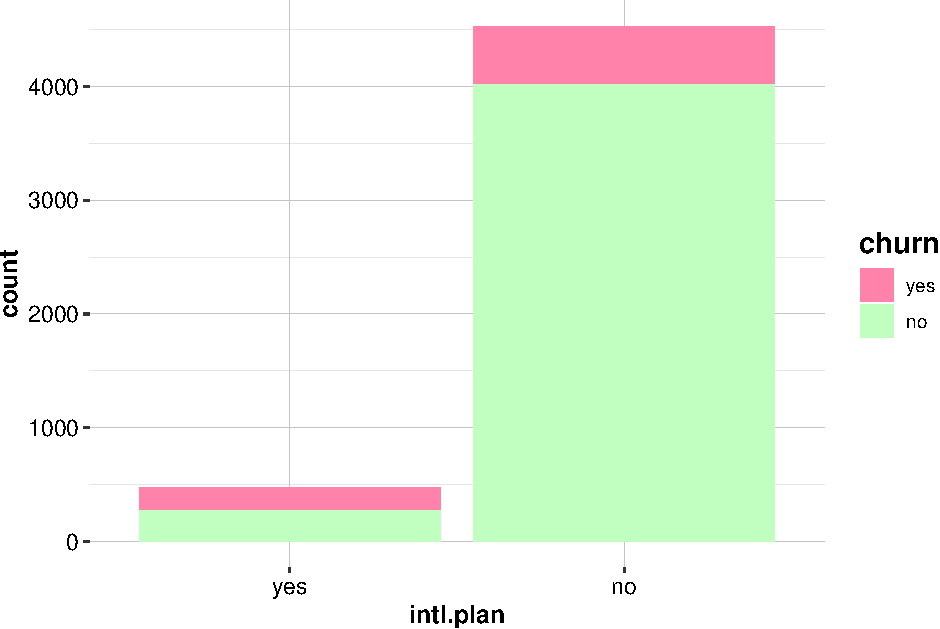
\includegraphics{EDA_files/figure-latex/unnamed-chunk-5-1} \end{center}

The bar plot above presents the distribution of the target variable \passthrough{\lstinline!churn!}, which indicates whether a customer has churned (left the company). The plot reveals that the dataset is imbalanced, with more customers staying (\passthrough{\lstinline!churn = "no"!}) than leaving (\passthrough{\lstinline!churn = "yes"!}); It presents that the proportion of churner (\passthrough{\lstinline!churn = "yes"!}) is 1.4 percent while the proportion of non-churner (\passthrough{\lstinline!churn = "yes"!}) is 8.6 percent. This information is crucial for building predictive models, as imbalance can affect model performance and accuracy. Besides, one of our objective is \emph{to reduce the proportion of churners}. For this we need \emph{to identify patterns in the data related to customer churn}, so we need to investigate the relationship between the target variable and other predictors.

The primary purpose of exploratory data analysis (EDA) is to gain a thorough understanding of the variables in the dataset by examining the distributions of categorical variables, analyzing histograms of numerical variables, and exploring relationships between variables. While EDA focuses on uncovering patterns and understanding data structure, our ultimate goal for this data mining project is to develop a predictive model that identifies customers likely to churn, or switch to a competitor. Today's data analysis tools allow us to familiarize ourselves with the dataset and investigate potential associations with churn, helping us explore the data while keeping the project's objective in mind. We begin by examining the categorical variables and their relationship to churn, as this foundational analysis will guide us in building an effective predictive model.

We begin our analysis with the \passthrough{\lstinline!intl.plan!} (International Plan) variable, which indicates whether a customer has subscribed to an international calling plan. As a binary variable, it provides two categories---those with an international plan and those without. To explore the relationship between this feature and customer churn, we can use bar plots to visualize the distribution of churners and non-churners based on the international plan selection:

\begin{lstlisting}[language=R]
ggplot(data = churn) + 
  geom_bar(aes(x = intl.plan, fill = churn)) +
  scale_fill_manual(values = c("palevioletred1", "darkseagreen1")) 

ggplot(data = churn) + 
  geom_bar(aes(x = intl.plan, fill = churn), position = "fill") +
  scale_fill_manual(values = c("palevioletred1", "darkseagreen1")) 
\end{lstlisting}

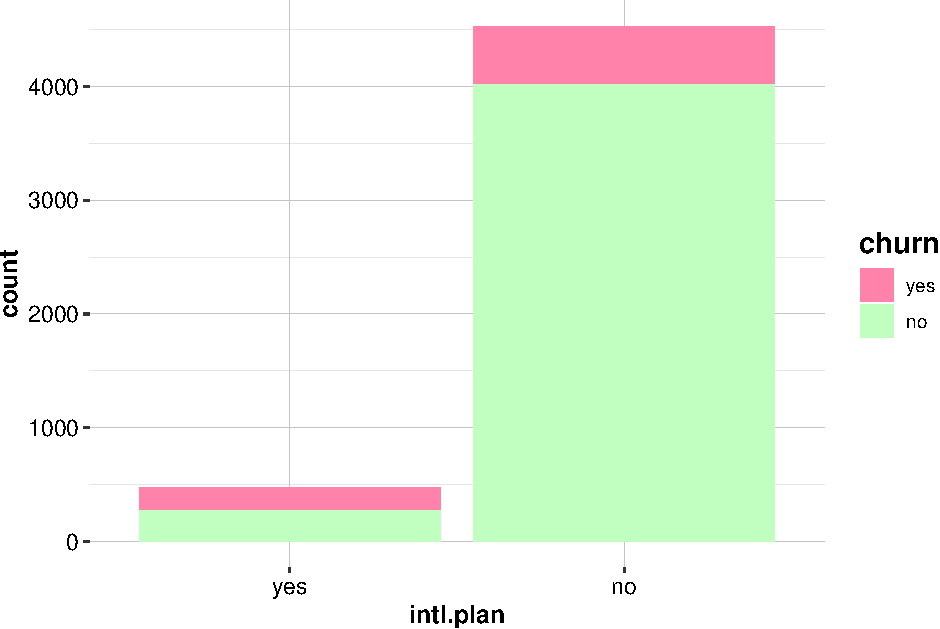
\includegraphics[width=0.5\linewidth]{EDA_files/figure-latex/unnamed-chunk-6-1} 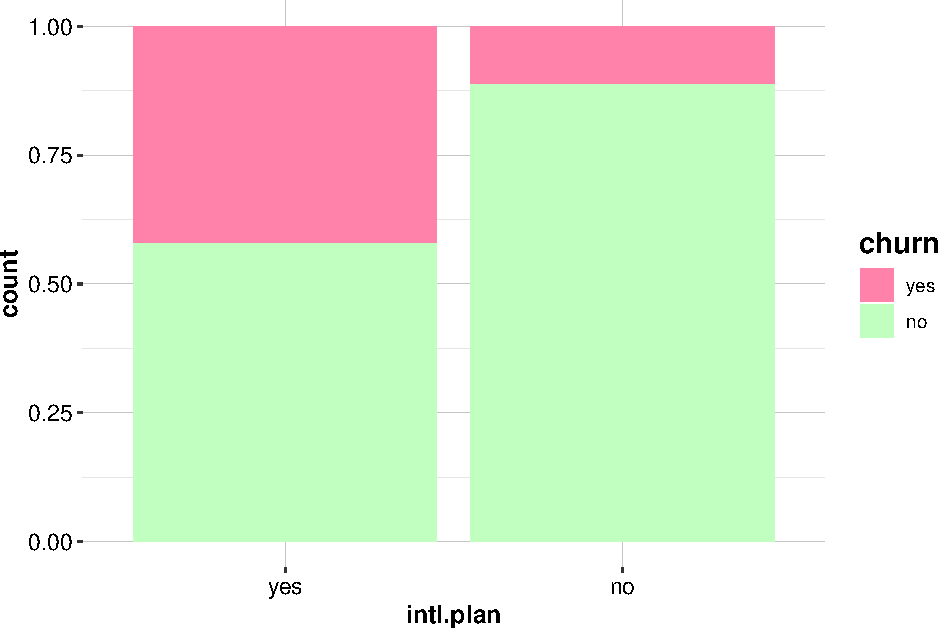
\includegraphics[width=0.5\linewidth]{EDA_files/figure-latex/unnamed-chunk-6-2}

The first plot (on the left) shows the distribution of churners and non-churners across the two categories of the international plan. This plot allows us to directly compare the raw counts of churners and non-churners among customers with and without the plan. The second plot (on the right) displays the proportions of churners and non-churners within each category, with the y-axis scaled from 0 to 1. This proportion plot is particularly useful for comparing churn rates, as it normalizes for differences in group sizes. From these plots, we observe that customers with the international plan have a noticeably higher churn rate than those without it, suggesting a potential link between the international plan and customer attrition.

To quantify this relationship, we can examine a contingency table, which provides a detailed breakdown of churners and non-churners by international plan status. Since both \passthrough{\lstinline!intl.plan!} and \passthrough{\lstinline!churn!} are categorical variables, this table helps us summarize and compare the distribution across categories:

\begin{lstlisting}[language=R]
addmargins(table(churn$churn, churn$intl.plan, 
                 dnn = c("Churn", "International Plan")))
        International Plan
   Churn  yes   no  Sum
     yes  199  508  707
     no   274 4019 4293
     Sum  473 4527 5000
\end{lstlisting}

This contingency table shows the count of churners and non-churners for customers with and without the international plan. If we wish to view these counts as proportions, we can use the \passthrough{\lstinline!prop.table()!} function, which converts the counts into percentages and provides a clearer view of the relative churn rates within each category.

In summary, our exploratory analysis of the International Plan variable suggests two key takeaways:

\begin{enumerate}
\def\labelenumi{\arabic{enumi}.}
\tightlist
\item
  There is a clear association between having an international plan and an increased likelihood of churn. This may warrant further investigation to understand what aspects of the international plan could be driving customers away.
\item
  We can expect that the international plan variable will likely play an important role in any predictive model for churn, as it shows a strong relationship with the target variable. Whatever data mining algorithm we choose, it's probable that the model will include this feature as a significant predictor of customer churn.
\end{enumerate}

By examining the relationship between the international plan and churn, we've taken an important first step toward understanding the dataset and identifying potential predictors of customer attrition. This initial analysis lays the groundwork for building predictive models that can help companies proactively address factors influencing churn and ultimately improve customer retention.

Next, we'll continue our exploration by investigating the \passthrough{\lstinline!voice.plan!} (Voice Mail Plan) variable and its relationship to churn. Applying a similar approach---visualizing and summarizing the data---will provide additional insights into customer behavior and allow us to refine our understanding of the dataset. To start, we visualize the distribution of churners and non-churners based on the Voice Mail Plan with the following bar plots:

\begin{lstlisting}[language=R]
ggplot(data = churn) + 
  geom_bar(aes(x = voice.plan, fill = churn)) +
  scale_fill_manual(values = c("palevioletred1", "darkseagreen1")) 

ggplot(data = churn) + 
  geom_bar(aes(x = voice.plan, fill = churn), position = "fill") +
  scale_fill_manual(values = c("palevioletred1", "darkseagreen1")) 
\end{lstlisting}

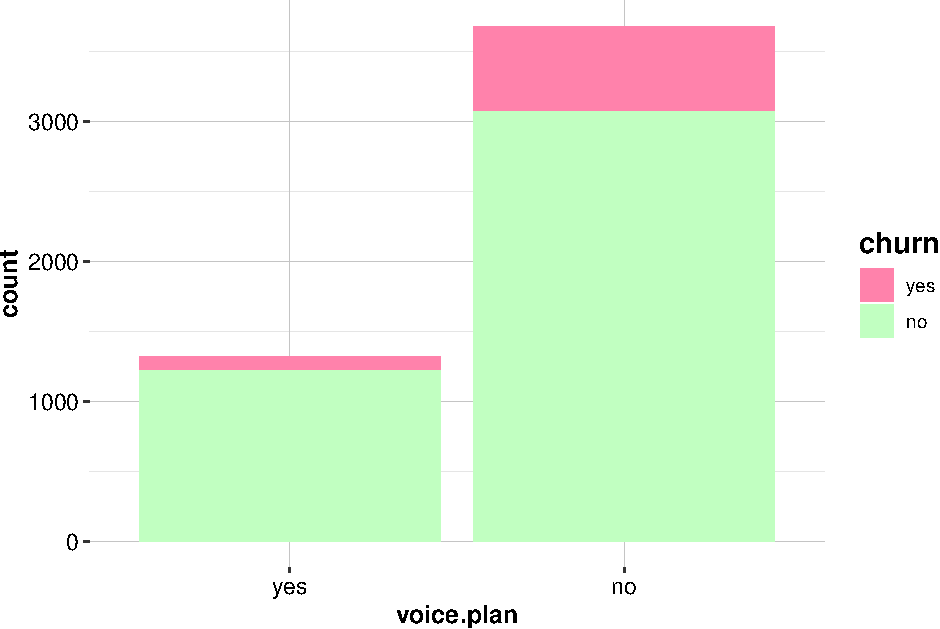
\includegraphics[width=0.5\linewidth]{EDA_files/figure-latex/unnamed-chunk-8-1} 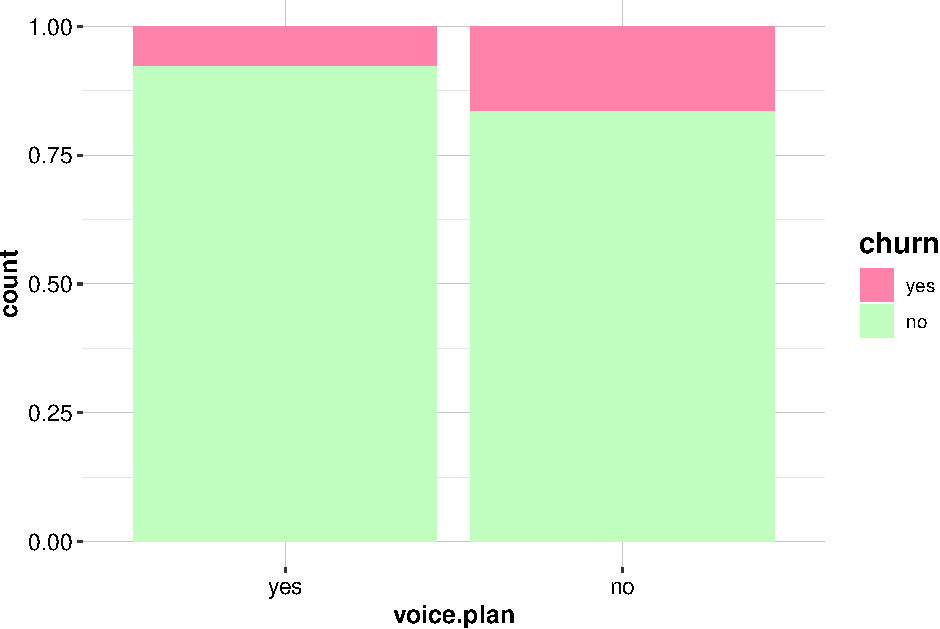
\includegraphics[width=0.5\linewidth]{EDA_files/figure-latex/unnamed-chunk-8-2}

The first plot (on the left) shows the raw counts of churners and non-churners among customers with and without a Voice Mail Plan, while the second plot (on the right) displays the proportions. From these plots, we observe that customers without a Voice Mail Plan appear more likely to churn than those who have opted in for this feature.

To quantify this observation, we can create a contingency table to summarize the counts of churners and non-churners by Voice Mail Plan status:

\begin{lstlisting}[language=R]
addmargins(table(churn$churn, churn$voice.plan, dnn = c("Churn", "Voice Mail Plan")))
        Voice Mail Plan
   Churn  yes   no  Sum
     yes  102  605  707
     no  1221 3072 4293
     Sum 1323 3677 5000
\end{lstlisting}

This table shows the number of churners and non-churners for customers with and without a Voice Mail Plan. For example, it reveals that 102 customers with a Voice Mail Plan did not churn, while 1221 did. Similarly, we can see the counts for customers without a Voice Mail Plan. The higher proportion of churners among those without a Voice Mail Plan suggests that this feature may indeed be a relevant predictor of customer attrition.

In summary, this EDA on the Voice Mail Plan variable suggests two key takeaways:

\begin{enumerate}
\def\labelenumi{\arabic{enumi}.}
\tightlist
\item
  Enhancing the Voice Mail Plan or encouraging more customers to subscribe to it may help improve customer retention, as the plan seems to be associated with lower churn rates.
\item
  We can expect that the Voice Mail Plan variable will likely contribute meaningfully to any predictive model we develop for churn, though its influence may not be as strong as that of the International Plan.
\end{enumerate}

These insights reinforce the importance of EDA in uncovering patterns that inform both strategic decisions and model-building efforts, helping companies address churn more effectively.

\section{Investigating Numerical Variables}\label{investigating-numerical-variables}

Next, we turn to an exploration of the numeric predictive variables. Refer back to summary statistics of the various predictors. We start with the variable \passthrough{\lstinline!service.calls!} (Customer Service Calls), which represents the number of calls made to customer service. This variable is numerical and discrete, making it suitable for histogram analysis. We can use histograms to visualize the distribution of customer service calls as follows:

\begin{lstlisting}[language=R]
ggplot(data = churn) +
  geom_histogram(aes(x = customer.calls), 
                 bins = 10, fill = "skyblue", color = "black")
\end{lstlisting}

\begin{center}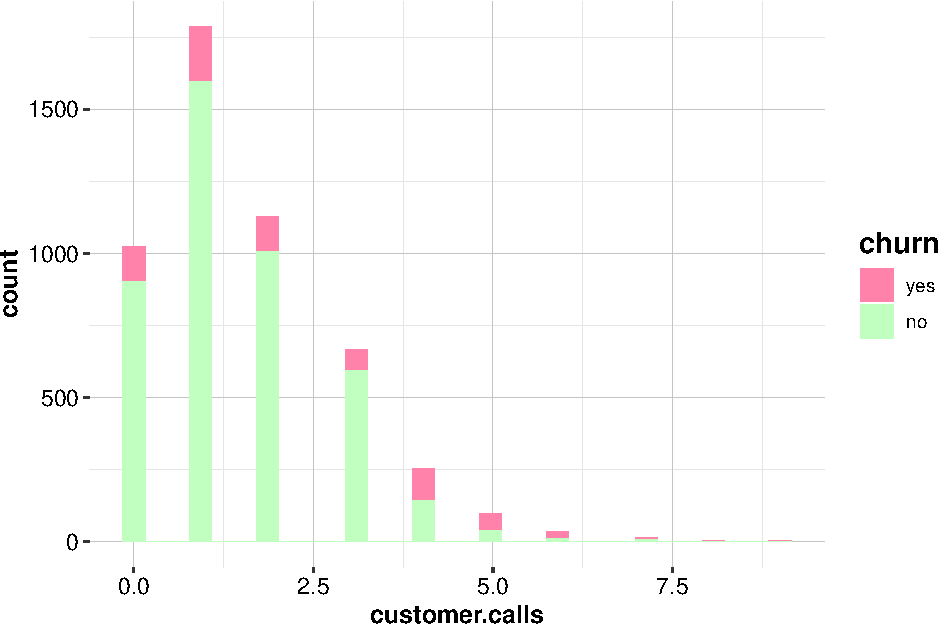
\includegraphics{EDA_files/figure-latex/unnamed-chunk-10-1} \end{center}

The histogram above displays the distribution of customer service calls, with the x-axis representing the number of calls and the y-axis showing the count of customers. This visualization allows us to observe the frequency of different call counts. For example, we can see that the range of calls is between 0 and maximum 9 with the majority of customers calls to customer service numeric times and that the distribution is right-skewed, with a long tail to the right. This skewness indicates that a few customers made a large number of calls, potentially signaling dissatisfaction or issues that need to be addressed.

The initial histogram gives a basic overview of the distribution of customer service calls, but to investigate its association with churn, we need to incorporate the target variable in the visualization. Overlaying the histogram with the target variable provides a clearer picture of how this predictor relates to churn. By coloring the histogram bars according to churn status, we can better discern patterns that might suggest a relationship between customer service calls and the likelihood of churn. Here's the code to create these overlay histograms:

\begin{lstlisting}[language=R]
ggplot(data = churn) +
  geom_histogram(aes(x = customer.calls, fill = churn), position = "stack") +
  scale_fill_manual(values = c("palevioletred1", "darkseagreen1")) 
  
ggplot(data = churn) +
  geom_histogram(aes(x = customer.calls, fill = churn), position = "fill") +
  scale_fill_manual(values = c("palevioletred1", "darkseagreen1")) 
\end{lstlisting}

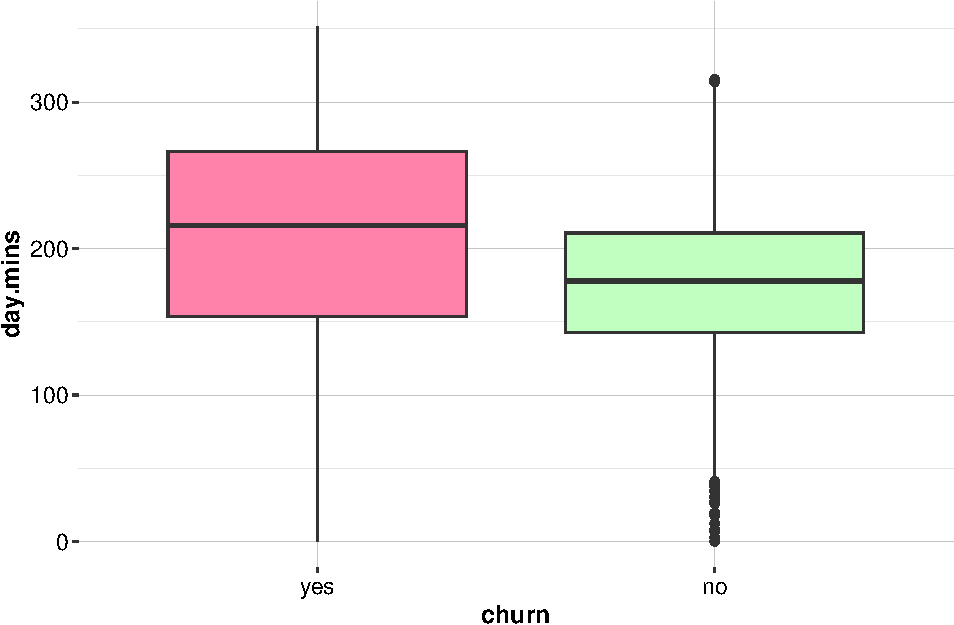
\includegraphics[width=0.5\linewidth]{EDA_files/figure-latex/unnamed-chunk-11-1} 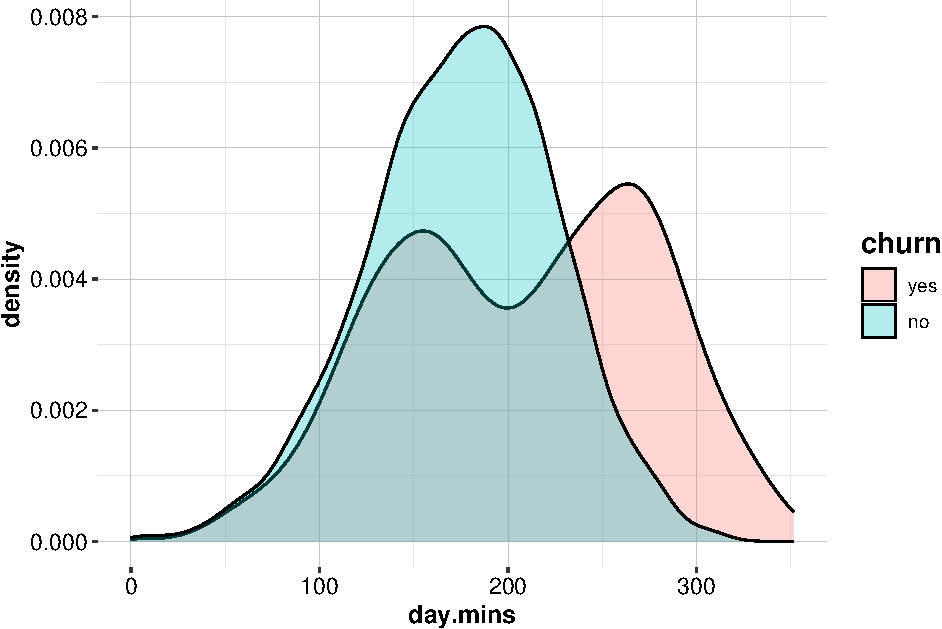
\includegraphics[width=0.5\linewidth]{EDA_files/figure-latex/unnamed-chunk-11-2}

The first plot (left) shows the distribution of churners and non-churners for each level of customer service calls, while the second plot (right) presents these values as proportions within each call count. In the left plot, there is a suggestion that churn is more prevalent among customers with higher call counts, but the pattern isn't immediately clear. The normalized histogram on the right, however, makes the relationship much more apparent by standardizing each bar to a height of 1, allowing us to easily compare the relative proportions of churners within each call level.

From the normalized plot, we can see a striking pattern: customers who have made three or fewer calls to customer service have a notably lower churn rate than those who have made four or more calls. This visualization indicates that frequent customer service interactions are a strong indicator of churn risk.

This analysis of the customer service calls variable suggests the following actionable insights:

\begin{enumerate}
\def\labelenumi{\arabic{enumi}.}
\tightlist
\item
  \textbf{Customer Retention Strategy}: Monitor the number of customer service calls closely. By the third call, it may be beneficial to offer specialized retention incentives, as the likelihood of churn increases significantly after the fourth call.
\item
  \textbf{Predictive Modeling}: We should expect that the number of customer service calls will be an important predictor in any model designed to forecast churn, as it appears to be highly indicative of customer dissatisfaction.
\end{enumerate}

Let's now examine the remaining numerical variables in the dataset, starting with \passthrough{\lstinline!day.mins!} (Day Minutes). Since \passthrough{\lstinline!day.mins!} is a continuous variable, we can visualize its distribution using both a box plot and a density plot, each providing different insights. Below, we present these two plots side by side:

\begin{lstlisting}[language=R]
ggplot(data = churn) +
    geom_boxplot(aes(x = churn, y = day.mins), 
                 fill = c("palevioletred1", "darkseagreen1"))

ggplot(data = churn) +
    geom_density(aes(x = day.mins, fill = churn), alpha = 0.3)
\end{lstlisting}

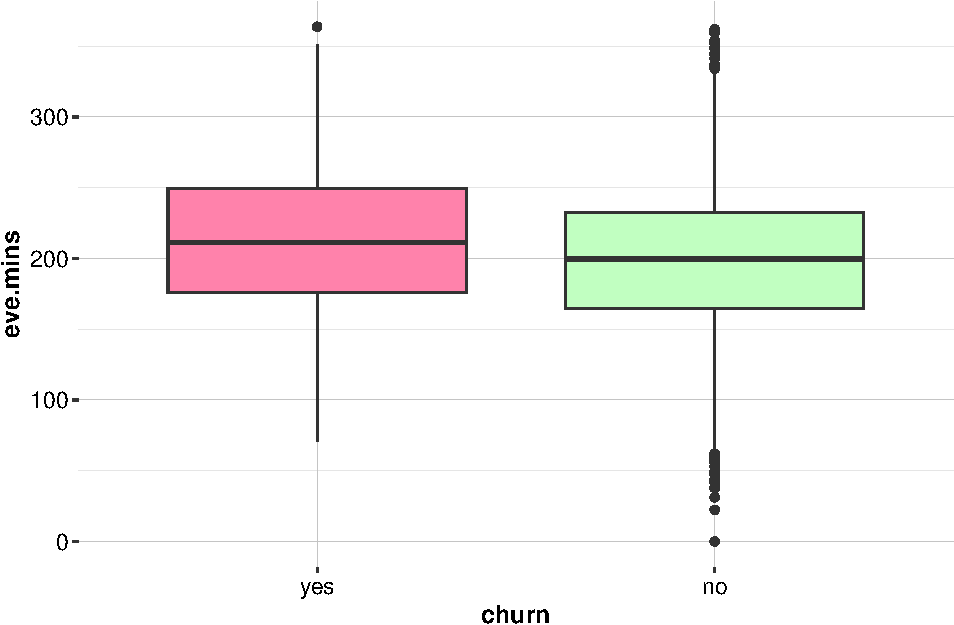
\includegraphics[width=0.5\linewidth]{EDA_files/figure-latex/unnamed-chunk-12-1} 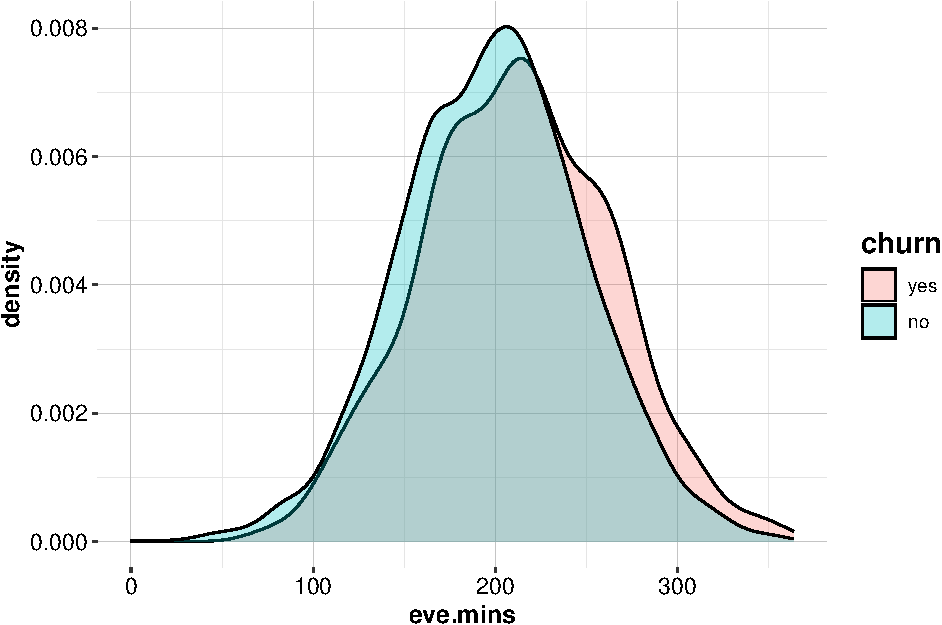
\includegraphics[width=0.5\linewidth]{EDA_files/figure-latex/unnamed-chunk-12-2}

The box plot on the left allows us to compare the distribution of \passthrough{\lstinline!day.mins!} between churners and non-churners, highlighting any differences in median, spread, and potential outliers. The density plot on the right provides a smooth visualization of the distribution, making it easier to spot patterns in day usage across both groups.

From these plots, we observe that high day-minute users are more likely to churn. The density plot, in particular, shows a noticeable peak among churners at higher \passthrough{\lstinline!day.mins!} values, suggesting that heavy daytime usage may be linked to customer dissatisfaction or unmet needs.

This analysis suggests the following actions:

\begin{enumerate}
\def\labelenumi{\arabic{enumi}.}
\tightlist
\item
  \textbf{Monitor High Day-Minute Users}: Track customers whose day-minute usage exceeds 200 minutes, as these high-usage customers appear to be at greater risk of churning.
\item
  \textbf{Investigate Reasons for Churn Among Heavy Users}: Explore why heavy daytime users are more inclined to leave. Are they experiencing issues with service quality, pricing, or value?
\item
  \textbf{Include \passthrough{\lstinline!day.mins!} in Churn Prediction Models}: Given its apparent predictive power, \passthrough{\lstinline!day.mins!} should be considered as a key feature in any churn prediction model, as it may help identify high-risk customers.
\end{enumerate}

In summary, analyzing \passthrough{\lstinline!day.mins!} has provided valuable insights into customer behavior, highlighting an opportunity to improve customer retention by focusing on heavy daytime users. By including this variable in predictive models, we can enhance the model's accuracy and take proactive steps to reduce churn among high-usage customers.

To examine the relationship between the \passthrough{\lstinline!eve.mins!} (Evening Minutes) variable and churn, we can use both a box plot and a density plot to visualize the distribution of evening minutes for churners and non-churners:

\begin{lstlisting}[language=R]
ggplot(data = churn) +
    geom_boxplot(aes(x = churn, y = eve.mins), fill = c("palevioletred1", "darkseagreen1"))

ggplot(data = churn) +
    geom_density(aes(x = eve.mins, fill = churn), alpha = 0.3)
\end{lstlisting}

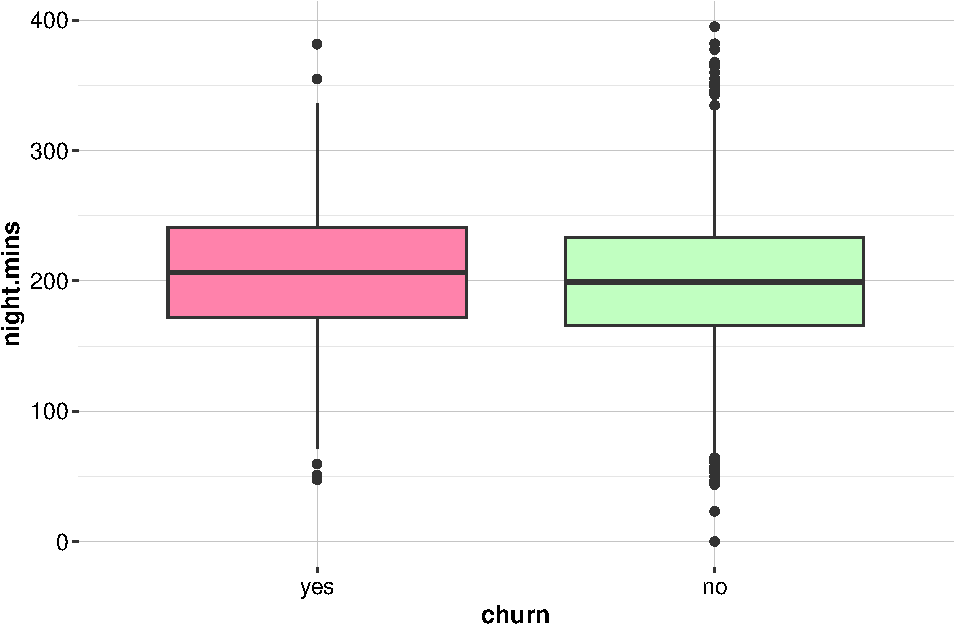
\includegraphics[width=0.5\linewidth]{EDA_files/figure-latex/unnamed-chunk-13-1} 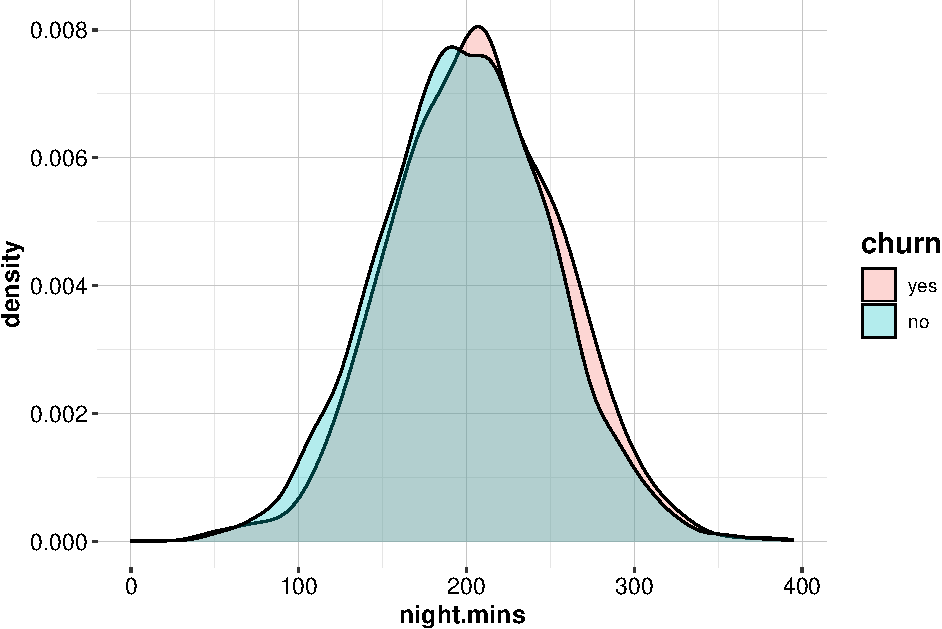
\includegraphics[width=0.5\linewidth]{EDA_files/figure-latex/unnamed-chunk-13-2}

The box plot (left) and density plot (right) offer different perspectives on the distribution of evening minutes across the churn and non-churn groups. The box plot provides a summary of the median, interquartile range, and potential outliers, while the density plot shows the overall shape of the distribution for each group.

From these plots, we observe a slight tendency for customers with higher evening minutes to have a greater likelihood of churning. However, this pattern is subtle, and the graphical evidence alone is not strong enough to make a definitive conclusion about the relationship between evening usage and churn. In situations like this, where the visual trends are ambiguous, it's prudent to withhold policy recommendations until we have more robust evidence from statistical analyses or predictive models.

In summary, while there may be an association between evening usage and churn, we need additional evidence before drawing conclusions. Proceeding with caution is essential in data analysis, particularly when visual trends are weak or uncertain. A data-driven approach will allow us to validate these findings before making any data-backed recommendations for policy or customer retention strategies.

To explore the relationship between \passthrough{\lstinline!night.mins!} (Night Minutes) and churn, we can visualize the data using a box plot and a density plot:

\begin{lstlisting}[language=R]
ggplot(data = churn) +
    geom_boxplot(aes(x = churn, y = night.mins), fill = c("palevioletred1", "darkseagreen1"))

ggplot(data = churn) +
    geom_density(aes(x = night.mins, fill = churn), alpha = 0.3)
\end{lstlisting}

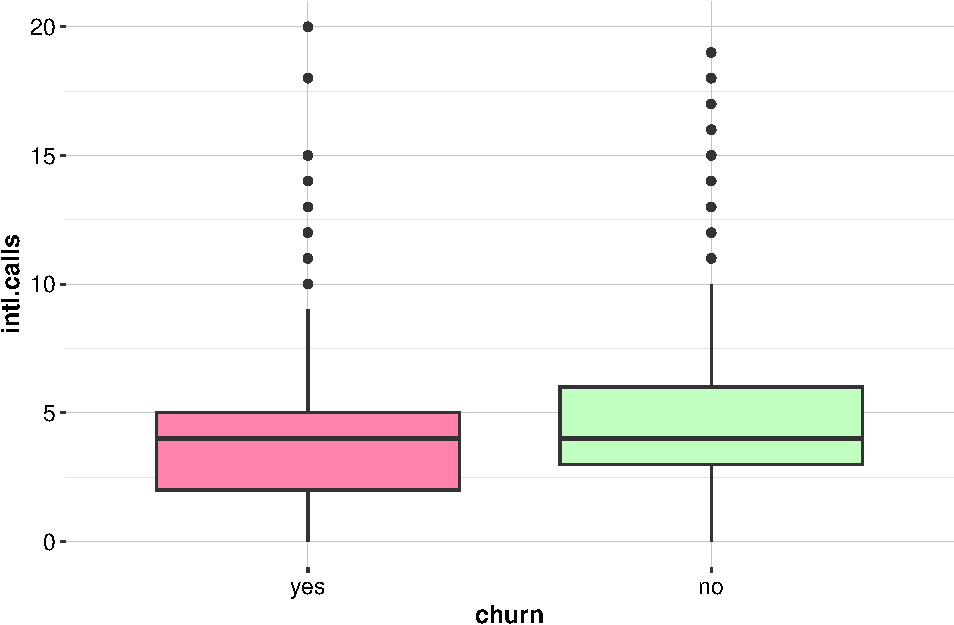
\includegraphics[width=0.5\linewidth]{EDA_files/figure-latex/unnamed-chunk-14-1} 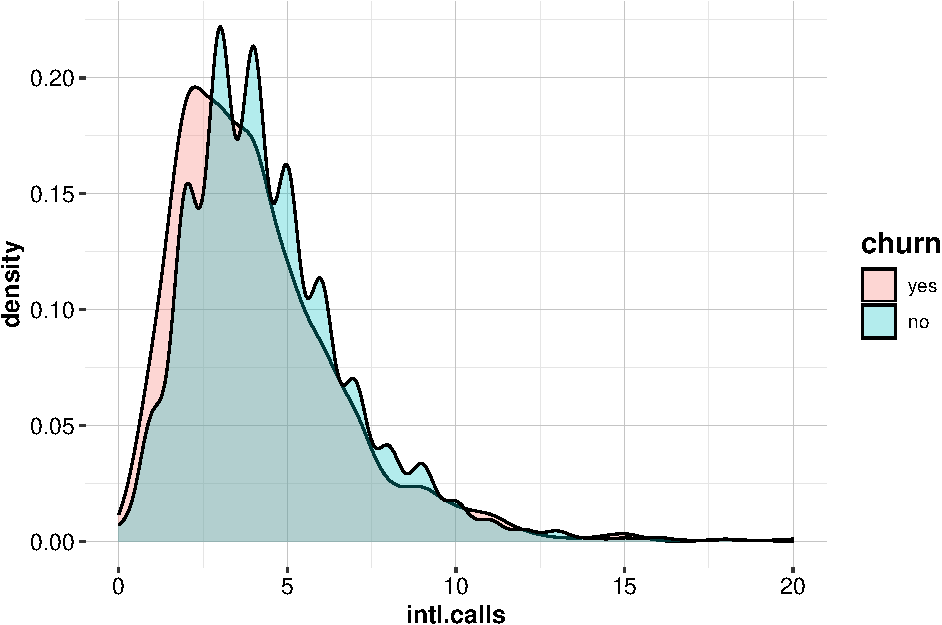
\includegraphics[width=0.5\linewidth]{EDA_files/figure-latex/unnamed-chunk-14-2}

The box plot (on the left) and density plot (on the right) both suggest that there is little to no discernible association between churn and night minutes. The distributions of night minutes for churners and non-churners are quite similar, with no significant differences in median, spread, or overall shape. This lack of variation implies that \passthrough{\lstinline!night.mins!} may not be a strong predictor of customer churn.

In fact, this pattern of minimal association with churn appears to hold for several of the remaining numeric variables in the dataset. While we have examined only a subset of variables in detail, you may wish to further investigate others to confirm whether they exhibit any meaningful relationship with churn. Identifying variables with little or no predictive value is a valuable part of the EDA process, as it allows us to focus on features that are more likely to enhance our model's accuracy.

Ultimately, EDA serves as a guide to prioritize which features are worth closer examination and inclusion in predictive modeling. For features like \passthrough{\lstinline!night.mins!}, where EDA indicates no obvious link to churn, we might consider excluding them from our final model or keeping them as secondary variables.

\textbf{Note:} The absence of an obvious association between a predictor and the target variable during EDA is not, on its own, a sufficient reason to exclude that predictor from our model. For instance, although the box plot and density plot for \passthrough{\lstinline!night.mins!} (Night Minutes) show no clear visual relationship with churn, this does not necessarily mean that \passthrough{\lstinline!night.mins!} lacks predictive value. Data mining models may still uncover useful patterns involving this variable, particularly if it interacts with other features or contributes to complex, higher-dimensional associations. Therefore, unless there is a compelling reason to discard a variable outright, it is generally best to include it in the initial stages of modeling and allow the model itself to determine its predictive importance.

As an example, while \passthrough{\lstinline!night.mins!} does not display a strong association with churn in the EDA visuals, further analysis using statistical tests may reveal otherwise. A t-test, for instance, could show a statistically significant difference in the mean number of Night Minutes between churners and non-churners (see Chapter 3 for details). This finding would suggest that \passthrough{\lstinline!night.mins!} may indeed have predictive power for identifying churn, even though this was not immediately apparent in the visualizations. Excluding the variable based solely on its lack of obvious association at the EDA stage could lead to a less accurate model, as subtle but meaningful patterns might go unrecognized.

To confirm whether any observed differences are statistically significant, we will delve into hypothesis testing and other statistical techniques in the next chapter. These methods fall under the domain of statistical inference and model building, extending beyond the scope of exploratory data analysis. We mention them here to emphasize that EDA is only one step in the modeling process; some variables may reveal their importance only under more formal analysis. For this reason, it's essential not to prematurely discard predictors simply because their relationship with the target variable isn't immediately apparent in EDA.

\section{Envestigating Multivarate Relationships}\label{envestigating-multivarate-relationships}

We examine potential multivariate associations between numeric variables and churn using scatter plots. While univariate exploration gives us insights into individual variables, multivariate graphics can reveal interaction effects that may not be apparent when examining variables in isolation.

For instance, consider the scatter plot of \passthrough{\lstinline!day.mins!} (Day Minutes) versus \passthrough{\lstinline!eve.mins!} (Evening Minutes), with churn overlaid:

\begin{lstlisting}[language=R]
ggplot(data = churn) +
    geom_point(aes(x = eve.mins, y = day.mins, color = churn), size = 0.7, alpha = 0.8) +
    scale_color_manual(values = c("palevioletred1", "darkseagreen1")) +
    geom_abline(intercept = 400, slope = -0.6, color = "blue", size = 1)
\end{lstlisting}

\begin{center}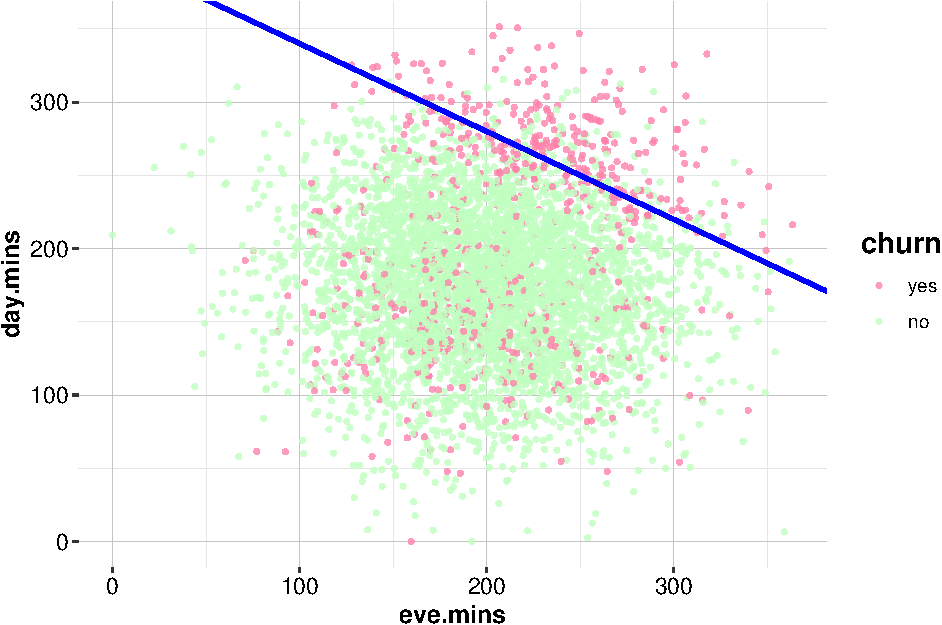
\includegraphics{EDA_files/figure-latex/unnamed-chunk-15-1} \end{center}

Notice the diagonal line partitioning the plot. This line, represented by the equation:

\[
\text{day.mins} = 400 - 0.6 \times \text{eve.mins}
\]

separates the upper-right section of the graph, where we observe a higher concentration of churners. This region, encompassing customers with both high day minutes and high evening minutes, appears to be a high-churn zone compared to the rest of the data.

To further investigate, we isolate this high-churn region and visualize the churn distribution within it:

\begin{lstlisting}[language=R]
sub_churn = subset(churn, (day.mins > 400 - 0.6 * eve.mins))

ggplot(data = sub_churn, aes(x = churn, label = scales::percent(prop.table(stat(count))))) +
    geom_bar(fill = c("palevioletred1", "darkseagreen1")) + 
    geom_text(stat = 'count', vjust = 0.2, size = 6)
\end{lstlisting}

\begin{center}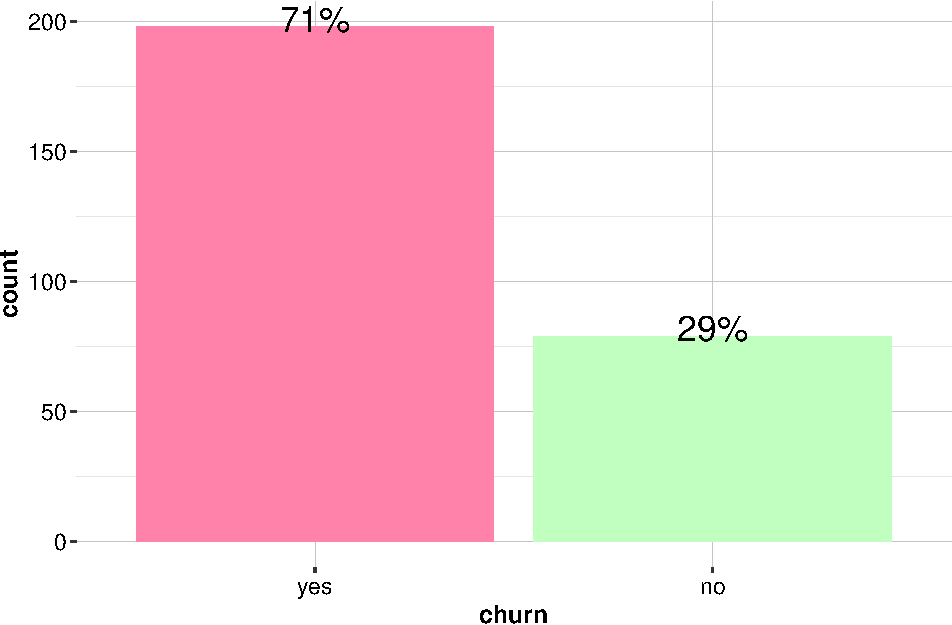
\includegraphics{EDA_files/figure-latex/unnamed-chunk-16-1} \end{center}

In this high-churn subset, the churn rate is approximately 29\%, which is significantly higher than the churn rate of 86\% observed across the entire dataset---around five times the overall churn rate. This stark increase in churn rate among customers with both high day and evening usage suggests a strong interaction effect that wasn't fully apparent in the univariate analyses.

Interestingly, while the univariate exploration of \passthrough{\lstinline!eve.mins!} alone did not clearly indicate a high churn rate, this multivariate analysis reveals that evening minutes do play a role in churn---particularly when combined with high day minutes. This demonstrates the value of multivariate exploration in uncovering hidden patterns and interactions, providing us with more nuanced insights into the factors influencing customer churn.

We can further investigate multivariate relationships by examining the scatter plot of \passthrough{\lstinline!customer.calls!} versus \passthrough{\lstinline!day.mins!}, with churn status overlaid:

\begin{lstlisting}[language=R]
ggplot(data = churn) +
  geom_point(aes(x = day.mins, y = customer.calls, color = churn), alpha = 0.8) +
  scale_color_manual(values = c("palevioletred1", "darkseagreen1"))
\end{lstlisting}

\begin{center}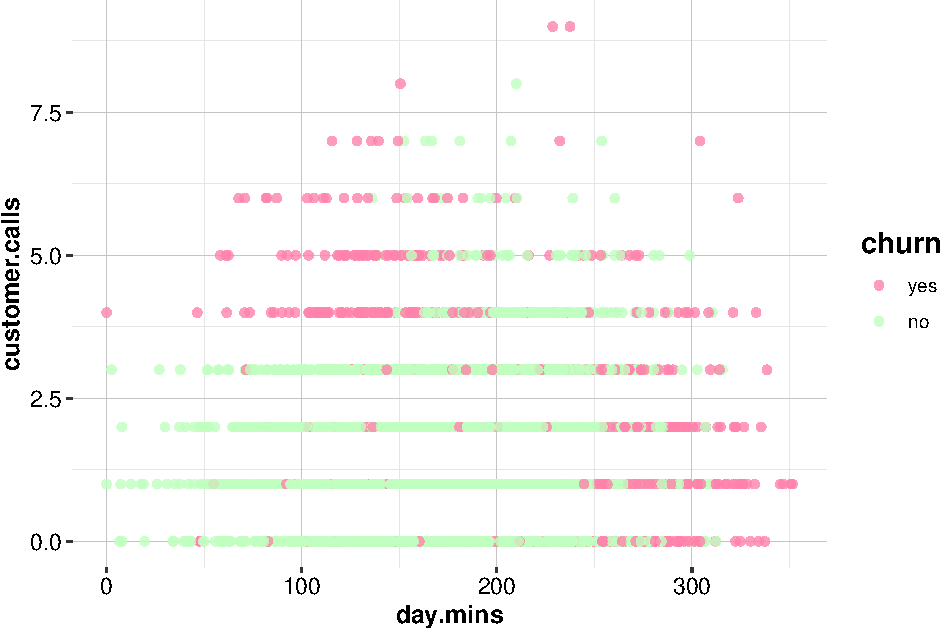
\includegraphics{EDA_files/figure-latex/unnamed-chunk-17-1} \end{center}

This plot reveals an interesting high-churn region in the upper left section, where customers have made numerous calls to customer service but have relatively low day minutes. This group of customers, characterized by frequent customer service interactions yet low usage, might represent a dissatisfied segment prone to leaving. Such insights would be difficult to uncover through univariate analysis alone, as they stem from the interaction between two variables rather than the behavior of any one variable in isolation.

In summary, our previous univariate analysis showed that customers who make many calls to customer service tend to have a higher churn rate. However, this scatter plot adds nuance to that finding. Among the high-call customers, those with high day minutes seem somewhat ``protected'' from churning---they are more likely to stay compared to those with lower day minutes. In other words, the upper right area of the plot, where day minutes are high and customer calls are also high, shows a lower churn rate than the upper left, where high customer calls coincide with low day minutes.

This interaction suggests that high usage (indicated by high day minutes) may offset the negative effect of frequent customer service calls, perhaps reflecting a more engaged or ``sticky'' customer segment. But how do we quantify these observations from the scatter plot?

In the next chapter, we'll delve into statistical techniques that allow us to rigorously test and quantify these multivariate relationships, determining whether they have significant predictive value for our churn model. This will help us transition from exploratory insights to actionable, data-driven decisions.

\subsection{Investigating Correlated Variables}\label{investigating-correlated-variables}

In data analysis, \textbf{correlation} measures the relationship between two variables---specifically, the extent to which one variable changes in relation to another. Correlation helps us understand whether increases or decreases in one variable are associated with increases or decreases in another. There are three main types of correlation outcomes: \textbf{positive correlation} (both variables move in the same direction), \textbf{negative correlation} (one variable increases as the other decreases), and \textbf{no correlation} (no clear relationship between the variables).

For example, if you've ever wondered whether the number of hours you study is related to your exam scores, you're thinking about correlation. A positive correlation would mean that more hours of studying are associated with higher scores, while a negative correlation would imply that more studying is associated with lower scores (which would be unusual, but not impossible). Correlation doesn't imply causation, but it can reveal interesting associations worth exploring.

The strength and direction of a linear relationship between two variables \(x\) and \(y\) can be quantified using the \textbf{correlation coefficient} \(r\). This value ranges from -1 to 1:
- \textbf{\(r = 1\)} indicates a perfect positive correlation, where increases in \(x\) are always associated with proportional increases in \(y\).
- \textbf{\(r = -1\)} indicates a perfect negative correlation, where increases in \(x\) are always associated with proportional decreases in \(y\).
- \textbf{\(r = 0\)} suggests no linear relationship between \(x\) and \(y\).

Below, Figure \ref{fig:correlation} shows examples of different correlation coefficients.

\begin{figure}

{\centering 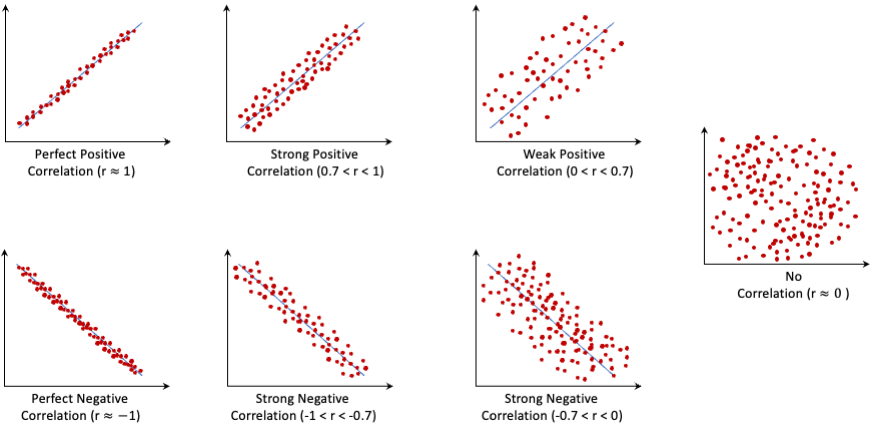
\includegraphics[width=1\linewidth]{images/correlation} 

}

\caption{Example scatterplots showing different correlation coefficients.}\label{fig:correlation}
\end{figure}

In large datasets---common in data science---even small values of \(r\) may be statistically significant. For datasets with over 1000 records, weak correlations (e.g., \(-0.1 \leq r \leq 0.1\)) can still hold statistical significance, though they may not always have practical importance. When evaluating correlations during exploratory data analysis (EDA), it's essential to consider both statistical and practical implications.

Using highly correlated predictors in a model can lead to several issues:
- \textbf{Overemphasis on Certain Data Patterns}: Strongly correlated predictors can cause certain patterns in the data to dominate the model's learning, potentially leading to biased outcomes.
- \textbf{Instability and Multicollinearity}: Highly correlated predictors introduce redundancy, which can destabilize models and make interpretation difficult. This problem, known as \textbf{multicollinearity}, is especially problematic in linear models and can result in unreliable coefficient estimates.

However, just because two variables are correlated doesn't mean that one should be automatically excluded from the model. Instead, during EDA, it's helpful to adopt a systematic approach for managing correlated variables.

To handle correlated variables effectively during EDA, consider the following strategies:

\begin{enumerate}
\def\labelenumi{\arabic{enumi}.}
\item
  \textbf{Identify Perfectly Correlated Variables}: If two variables have a perfect correlation (i.e., \(r = 1.0\) or \(r = -1.0\)), they contain identical information. Including both in the model would be redundant, so retaining only one is sufficient.
\item
  \textbf{Group Highly Correlated Variables}: Identify clusters of variables that are strongly correlated with each other. Later, during the modeling phase, you can apply \textbf{dimension reduction} techniques, such as \textbf{Principal Component Analysis (PCA)}, to combine these correlated variables into a smaller set of uncorrelated components. This approach reduces redundancy while retaining essential information.
\item
  \textbf{Consider Practical Relevance}: Correlation alone should not dictate variable inclusion or exclusion. For example, if two predictors are highly correlated but both have practical significance (e.g., \passthrough{\lstinline!age!} and \passthrough{\lstinline!years of experience!}), you may choose to retain both and evaluate their impact during the modeling phase.
\end{enumerate}

\begin{quote}
\textbf{Note}: This strategy applies to correlations among predictor variables, not between predictors and the target variable. Strong correlations between a predictor and the target variable are often desirable, as they suggest that the predictor may be informative for modeling the target.
\end{quote}

By following these steps, you can reduce the risk of multicollinearity and redundancy, helping to ensure that your models are both reliable and interpretable. This approach allows EDA to inform a thoughtful, data-driven selection of variables as you move into the modeling phase.

Let's apply this process to our dataset. For each of the categories \textbf{day}, \textbf{evening}, \textbf{night}, and \textbf{international}, we have three variables: \textbf{minutes}, \textbf{calls}, and \textbf{charge}. According to the data description, the \textbf{charge} variables are likely calculated based on \textbf{minutes} and \textbf{calls} for each time period, which would naturally result in high correlations between them. To verify this, we'll compute the correlation matrix for these variables and visualize it using a correlation plot.

\begin{lstlisting}[language=R]
library(ggcorrplot) # For correlation plots (ggcorrplot)
variable_list = c("intl.mins",  "intl.calls",  "intl.charge", 
                  "day.mins",   "day.calls",   "day.charge",
                  "eve.mins",   "eve.calls",   "eve.charge",
                  "night.mins", "night.calls", "night.charge")

cor_matrix = cor(churn[, variable_list])

ggcorrplot(cor_matrix, type = "lower", lab = TRUE, lab_size = 3)
\end{lstlisting}

\begin{center}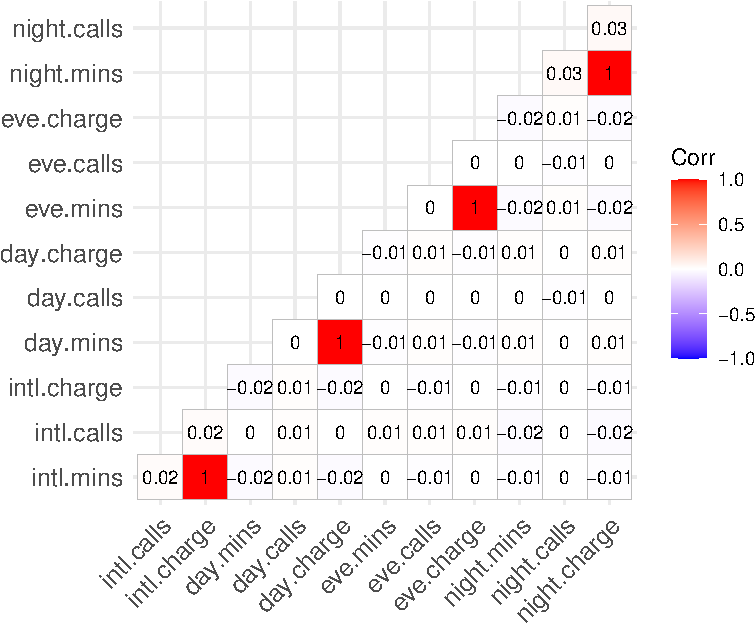
\includegraphics{EDA_files/figure-latex/unnamed-chunk-18-1} \end{center}

The correlation matrix reveals several key insights:
- \textbf{Perfect Correlations}: We observe perfect correlations (r = 1) between \passthrough{\lstinline!day.mins!} and \passthrough{\lstinline!day.charge!}, \passthrough{\lstinline!eve.mins!} and \passthrough{\lstinline!eve.charge!}, \passthrough{\lstinline!night.mins!} and \passthrough{\lstinline!night.charge!}, and \passthrough{\lstinline!intl.mins!} and \passthrough{\lstinline!intl.charge!}. This indicates that each \textbf{charge} variable is a direct linear function of the corresponding \textbf{minutes} variable.
- \textbf{No Correlation Between Minutes and Calls}: Interestingly, there is no significant correlation between \textbf{minutes} and \textbf{calls} within each time period (e.g., \passthrough{\lstinline!day.mins!} and \passthrough{\lstinline!day.calls!} are uncorrelated). While one might expect that customers making more calls would also spend more minutes on the phone, the data does not support this assumption.

Since \passthrough{\lstinline!day.charge!}, \passthrough{\lstinline!eve.charge!}, \passthrough{\lstinline!night.charge!}, and \passthrough{\lstinline!intl.charge!} are perfectly correlated with their respective \textbf{minutes} variables, we should remove one of each pair to avoid redundancy. We'll retain the \textbf{minutes} variables and eliminate the \textbf{charge} variables, thus reducing the number of predictors from 20 to 16. This helps prevent issues with multicollinearity and reduces the dimensionality of the data, which can improve model efficiency.

Had we proceeded to the modeling phase without identifying and addressing these correlations, our models could have produced unreliable results due to multicollinearity. High multicollinearity can distort the relationships between variables in a model, making it challenging to determine the true effect of each predictor. By removing redundant variables, we streamline the model and focus on the most meaningful predictors, leading to more stable and interpretable results.

\begin{quote}
\textbf{Important Note on Correlation vs.~Causation}: Remember that correlation does not imply causation. Just because two variables are correlated does not mean that one causes the other. Causation implies that changes in one variable directly result in changes in the other, while correlation simply indicates an association. Always be cautious in interpreting correlations, especially when considering them for causal inferences.
\end{quote}

In summary, by carefully investigating and addressing correlated variables during EDA, we enhance the reliability and interpretability of our models. This approach ensures that our modeling process is both data-driven and thoughtful, setting a solid foundation for the analyses and insights that follow.

\section{Key Findings and Insights}\label{key-findings-and-insights}

Through a thorough exploratory data analysis (EDA) of the churn dataset, we have gained valuable insights into the factors that may influence customer attrition. By examining each variable individually and in combination with others, we identified patterns and relationships that could inform predictive modeling and guide potential strategies for reducing churn. Here are the key takeaways from our analysis:

\begin{enumerate}
\def\labelenumi{\arabic{enumi}.}
\tightlist
\item
  \textbf{Redundant Variables}:
\end{enumerate}

\begin{itemize}
\tightlist
\item
  The \textbf{charge} fields (day, evening, night, and international) are perfectly correlated with their respective \textbf{minute} fields, as they are linear functions of those variables. To avoid redundancy and multicollinearity, we should exclude the charge fields from our analysis, retaining only the minute variables.
\item
  The \textbf{area code} and \textbf{state} fields appear to add little value and may be redundant or anomalous. Unless further clarification on their purpose is obtained, these fields should be omitted from the model.
\end{itemize}

\begin{enumerate}
\def\labelenumi{\arabic{enumi}.}
\setcounter{enumi}{1}
\tightlist
\item
  \textbf{Churn Insights}:
\end{enumerate}

\begin{itemize}
\tightlist
\item
  \textbf{International Plan}: Customers who have subscribed to the International Plan show a significantly higher churn rate. This suggests that the plan may not be meeting customer expectations, or it may be attracting a customer segment that is more prone to switching providers.
\item
  \textbf{Voice Mail Plan}: In contrast, customers with a Voice Mail Plan tend to churn less frequently, indicating that this service may enhance customer loyalty.
\item
  \textbf{Customer Service Calls}: A high number of customer service calls (four or more) is strongly associated with higher churn. Customers who have had to contact customer service multiple times may be experiencing unresolved issues or dissatisfaction, which ultimately leads them to leave.
\item
  \textbf{High Day and Evening Minutes}: Customers who have both high day minutes and high evening minutes churn at an elevated rate---up to six times the overall churn rate. This suggests that heavy usage during these time periods may correlate with dissatisfaction, possibly due to cost or quality issues.
\item
  \textbf{Combination of Low Day Minutes and High Customer Service Calls}: Customers who make frequent customer service calls but have relatively low day minutes also display a higher churn rate. This may indicate dissatisfaction among lower-usage customers who still face issues requiring support.
\item
  \textbf{International Calls}: Interestingly, customers with fewer international calls tend to churn more frequently than those who make more international calls. This could suggest that international usage may be a valuable service differentiator for certain customer segments.
\end{itemize}

\begin{enumerate}
\def\labelenumi{\arabic{enumi}.}
\setcounter{enumi}{2}
\tightlist
\item
  \textbf{Other Variables}:
\end{enumerate}

\begin{itemize}
\tightlist
\item
  For the remaining predictors, no obvious association with churn was identified through EDA. However, these variables are retained as potential inputs for downstream data mining models, as they may still contain useful predictive information in combination with other variables or within specific subsets of the data.
\end{itemize}

This exploratory analysis has highlighted the power of EDA in uncovering actionable insights before applying advanced modeling techniques. Without any sophisticated data mining algorithms, we have already identified several customer behaviors and attributes that correlate with churn. These findings provide a solid foundation for the next steps in our analysis, which will involve applying predictive modeling techniques to confirm and quantify the relationships we observed.

Additionally, the insights from EDA can be translated into actionable recommendations. For instance:
- The company could investigate the International Plan to understand why it correlates with higher churn and consider adjustments to make it more appealing.
- Specialized retention strategies could be deployed for customers who make frequent customer service calls, potentially offering tailored support to resolve their issues before they decide to leave.
- High-usage customers, particularly those with high day and evening minutes, could be targeted with incentives or loyalty programs to address any dissatisfaction related to cost or service quality.

By identifying and understanding these patterns, the company can take proactive steps to reduce churn and improve customer satisfaction, ultimately leading to a more loyal customer base.

\chapter{Statistical Inference and Hypothesis Testing}\label{chapter-statistics}

Statistical inference bridges the gap between \textbf{what we observe in a sample} and \textbf{what we want to understand about the population}. It allows us to assess whether the patterns we observed during EDA reflect true relationships in the broader population---or whether they're just the result of chance. In this chapter, we'll focus on the \textbf{practical side of statistical inference}: how to ask the right questions, apply the appropriate techniques, and use results to guide meaningful decisions.

The goals of statistical inference can be summarized into three fundamental tasks:

\begin{enumerate}
\def\labelenumi{\arabic{enumi}.}
\tightlist
\item
  \textbf{Estimating} unknown population characteristics, such as averages or proportions.\\
\item
  \textbf{Quantifying Uncertainty} to measure how confident we can be in our results.\\
\item
  \textbf{Testing Hypotheses} to evaluate whether observed patterns are statistically meaningful or simply due to random variation.
\end{enumerate}

These tasks lie at the heart of data analysis, providing the foundation for robust conclusions and data-driven decision-making. In this chapter, we'll explore these three pillars---estimation, uncertainty, and hypothesis testing---using intuitive explanations and practical examples.

But statistical inference isn't just about learning techniques---it's also about \textbf{critical thinking}. By the end of this chapter, you'll learn two essential skills:

\begin{itemize}
\tightlist
\item
  \textbf{How to detect when others are misusing statistics}, so you can identify misleading claims.\\
\item
  \textbf{How to avoid statistical missteps yourself}, or, if you're feeling mischievous, \emph{how to ``lie'' with statistics} effectively.
\end{itemize}

For those intrigued by the art of spotting statistical trickery, consider reading Darrell Huff's classic book, \href{https://www.goodreads.com/book/show/51291.How_to_Lie_with_Statistics}{\emph{How to Lie with Statistics}}. Although written with humor and journalistic insight, it offers timeless lessons in statistical skepticism---a valuable skill in an age of data overload.

Let's dive in and learn how to make inferences with confidence, curiosity, and just a touch of caution.

\section{Estimation: Using Data to Make Predictions}\label{estimation-using-data-to-make-predictions}

Estimation addresses the question: \emph{What can we infer about the population based on our sample?} For example, in the churn dataset, we may want to estimate:

\begin{itemize}
\tightlist
\item
  The \textbf{average number of customer service calls} among churners.
\item
  The \textbf{proportion of customers} subscribed to the International Plan.
\end{itemize}

Estimation comes in two main forms:

\begin{enumerate}
\def\labelenumi{\arabic{enumi}.}
\tightlist
\item
  \textbf{Point Estimation}: A single best guess for the population parameter (e.g., the sample mean or proportion).\\
\item
  \textbf{Interval Estimation}: A range of values (confidence interval) likely to contain the true population parameter.
\end{enumerate}

Let's explore some examples:

\begin{example}
\protect\hypertarget{exm:ex-est-churn-proportion}{}\label{exm:ex-est-churn-proportion}To estimate the \textbf{proportion of churners} in the dataset, we use the \textbf{sample proportion} as a point estimate for the population proportion. Here's how to calculate it in R:

\begin{lstlisting}[language=R]
# Calculate the proportion of churners
prop.table(table(churn$churn))["yes"]
      yes 
   0.1414
\end{lstlisting}

The proportion of churners in the dataset is \textbf{0.14}. This serves as our best single guess for the proportion of churners in the population.
\end{example}

\begin{example}
\protect\hypertarget{exm:ex-est-service-call}{}\label{exm:ex-est-service-call}let's estimate the \textbf{average number of customer service calls} for customers who churned. The \textbf{sample mean} acts as a point estimate for the population mean:

\begin{lstlisting}[language=R]
# Filter churners
churned_customers <- churn[churn$churn == "yes", ]

# Calculate the mean
mean_calls <- mean(churned_customers$customer.calls)
cat("Point Estimate: Average Customer Service Calls for Churners:", mean_calls)
   Point Estimate: Average Customer Service Calls for Churners: 2.254597
\end{lstlisting}

If the mean is \textbf{4 calls}, this is our best single guess for the average number of customer service calls among all churners in the population.
\end{example}

\begin{quote}
\textbf{Key Insight}: While point estimates are informative, they don't tell us how precise or reliable they are. For that, we turn to confidence intervals.
\end{quote}

\section{Quantifying Uncertainty: Confidence Intervals}\label{quantifying-uncertainty-confidence-intervals}

Confidence intervals (CIs) provide a way to \textbf{quantify uncertainty} by offering a range of plausible values for a population parameter. Instead of saying, ``The average number of customer service calls is 4,'' a confidence interval might state, ``We are 95\% confident that the true average is between 3.8 and 4.2.''

A confidence interval combines:

\begin{enumerate}
\def\labelenumi{\arabic{enumi}.}
\tightlist
\item
  A \textbf{point estimate} (e.g., sample mean or proportion).
\item
  A \textbf{margin of error}, which accounts for variability and uncertainty.
\end{enumerate}

The general form of a confidence interval is:

\[
\text{Point Estimate}  \pm \text{Margin of Error}
\]

For example, the confidence interval for a population mean is calculated as:

\[
\bar{x} \pm z_{\frac{\alpha}{2}} \times \left( \frac{s}{\sqrt{n}} \right),
\]
where the sample mean \(\bar{x}\) is the point estimate and the quantity \(z_{\frac{\alpha}{2}} \times \left( \frac{s}{\sqrt{n}} \right)\) is the margin of error. The z-score \(z_{\frac{\alpha}{2}}\) is determined by the desired confidence level (e.g., 1.96 for 95\% confidence), \(s\) is the sample standard deviation, and \(n\) = sample size.

This is visually represented in \ref{fig:confidence-interval}, showing the interval centered around the point estimate with the width determined by the margin of error.

\begin{figure}

{\centering 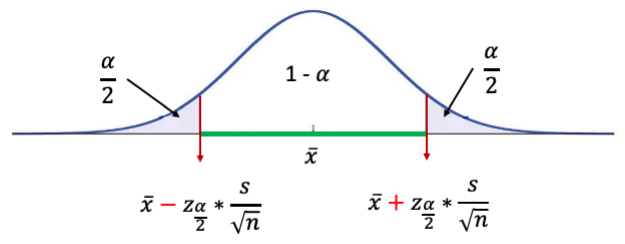
\includegraphics[width=0.8\linewidth]{images/confidence_interval} 

}

\caption{Confidence interval for the population mean. The interval is centered around the point estimate, with the width determined by the margin of error. The confidence level specifies the probability that the interval contains the true population parameter.}\label{fig:confidence-interval}
\end{figure}

Key Factors That Influence Confidence Intervals:

\begin{itemize}
\tightlist
\item
  \textbf{Sample Size}: Larger samples yield narrower intervals, increasing precision.\\
\item
  \textbf{Variability}: Higher variability in the data results in wider intervals.\\
\item
  \textbf{Confidence Level}: Higher confidence levels (e.g., 99\%) lead to wider intervals than lower levels (e.g., 90\%).
\end{itemize}

\begin{example}
\protect\hypertarget{exm:ex-confidence-service-call}{}\label{exm:ex-confidence-service-call}Let's calculate a 95\% confidence interval for the \textbf{average number of customer service calls} among churners:

\begin{lstlisting}[language=R]
# Calculate mean and standard error
mean_calls <- mean(churned_customers$customer.calls)
se_calls <- sd(churned_customers$customer.calls) / sqrt(nrow(churned_customers))

# Confidence Interval
z_score <- 1.96  # For 95% confidence
ci_lower <- mean_calls - z_score * se_calls
ci_upper <- mean_calls + z_score * se_calls

cat("95% Confidence Interval: [", ci_lower, ",", ci_upper, "]")
   95% Confidence Interval: [ 2.120737 , 2.388457 ]
\end{lstlisting}

If the confidence interval is \textbf{{[} 2.12, 2.39 {]}}, we are 95\% confident that the true average lies within this range.
\end{example}

For smaller sample sizes, use the \textbf{t-distribution} instead of the normal distribution. The t-distribution adjusts for the added uncertainty when estimating the population standard deviation. You can calculate confidence intervals for small samples in R using the \passthrough{\lstinline!t.test()!} function:

\begin{lstlisting}[language=R]
t.test(churned_customers$customer.calls, conf.level = 0.95)$conf.int
   [1] 2.120509 2.388685
   attr(,"conf.level")
   [1] 0.95
\end{lstlisting}

This approach automatically adjusts for the sample size and underlying variability in the data, making it a robust alternative to manual calculations.

\begin{quote}
\textbf{Interpretation}: If confidence intervals for different groups (e.g., churners vs.~non-churners) don't overlap significantly, it suggests meaningful differences in behavior between the groups.
\end{quote}

In summary, confidence intervals go beyond point estimates by providing a range of plausible values for the population parameter, helping us account for the uncertainty in our predictions. Narrower intervals indicate greater precision, which is achieved through larger sample sizes or lower variability in the data. Confidence levels, such as 95\%, quantify the degree of certainty that the interval contains the true population parameter. For smaller sample sizes, the t-distribution offers a more reliable approach by adjusting for the additional uncertainty inherent in limited data. Confidence intervals, therefore, serve as a critical tool for balancing precision and uncertainty in statistical inference.

\section{Hypothesis Testing}\label{hypothesis-testing}

Hypothesis testing is a cornerstone of inferential statistics, providing a structured framework for evaluating claims or assumptions about population parameters based on sample data. It allows us to assess whether observed patterns in the data are statistically significant or merely the result of random chance. This process lies at the heart of data-driven decision-making, empowering us to separate meaningful insights from noise.

At its core, hypothesis testing involves formulating two competing statements about a population parameter:

\begin{enumerate}
\def\labelenumi{\arabic{enumi}.}
\tightlist
\item
  \textbf{Null Hypothesis (\(H_0\))}: Represents the default assumption or status quo. For example, it might claim that there is no difference between two groups, no effect of a treatment, or no relationship between variables.
\item
  \textbf{Alternative Hypothesis (\(H_a\))}: Represents a competing claim that challenges the null hypothesis. For instance, it might state that there is a difference, an effect, or a relationship.
\end{enumerate}

The goal of hypothesis testing is to use evidence from the sample to decide whether to:

\begin{itemize}
\tightlist
\item
  \textbf{Reject \(H_0\)}: Conclude that the evidence supports \(H_a\), and the null hypothesis is unlikely to be true.
\item
  \textbf{Fail to reject \(H_0\)}: Conclude that there is insufficient evidence to refute \(H_0\), though this does not prove \(H_0\) to be true.
\end{itemize}

To make these decisions, we calculate a measure of evidence against the null hypothesis: the \textbf{p-value}.

The \textbf{p-value} quantifies the strength of the evidence against \(H_0\). Specifically, it represents the \textbf{probability of observing the sample data---or something more extreme---if the null hypothesis (\(H_0\)) were true}. Smaller p-values indicate stronger evidence against \(H_0\), as the observed data would be highly unlikely under the assumption that \(H_0\) is true. We interpret the p-value as follows:

\begin{itemize}
\tightlist
\item
  \textbf{Small p-value (e.g., \textless{} 0.05)}: The observed data is unlikely under \(H_0\). We reject \(H_0\) and conclude that there is evidence to support \(H_a\).
\item
  \textbf{Large p-value (e.g., \textgreater{} 0.05)}: The observed data is consistent with \(H_0\). We fail to reject \(H_0\) and conclude that there is insufficient evidence to support \(H_a\).
\end{itemize}

The \textbf{p-value} is compared against a predefined threshold known as the \textbf{significance level (\(\alpha\))}, which is commonly set at 0.05 (5\%). The significance level represents the maximum probability of committing a \textbf{Type I error}---rejecting \(H_0\) when it is actually true---that we are willing to tolerate. In certain fields, such as medicine or aerospace, where the cost of a Type I error is especially high, stricter thresholds (e.g., \(\alpha = 0.01\)) may be used to minimize this risk.

This leads us to a simple yet crucial takeaway, often referred to as the key decision rule for hypothesis testing. I often tell my students to remember this as the \textbf{core message} of the chapter:

\textbf{Reject \(H_0\) if the \(p\)-value \textless{} \(\alpha\)}.

Let's see how this works in practice:

\begin{itemize}
\tightlist
\item
  If \(p = 0.03\) and \(\alpha = 0.05\): \textbf{Reject \(H_0\)} because \(p < \alpha\). The evidence against \(H_0\) is strong enough to conclude that the alternative hypothesis is supported.
\item
  If \(p = 0.12\) and \(\alpha = 0.05\): \textbf{Fail to reject \(H_0\)} because \(p > \alpha\). The evidence is insufficient to refute \(H_0\), though this does not prove that \(H_0\) is true.
\end{itemize}

This decision-making framework ensures that hypothesis testing remains consistent, objective, and aligned with the predefined level of risk we are willing to accept for making errors.

While p-values are a useful tool, they are not without limitations:

\begin{enumerate}
\def\labelenumi{\arabic{enumi}.}
\tightlist
\item
  \textbf{p-value ≠ Importance}: A small p-value does not mean the effect is practically significant---it only indicates statistical significance. For example, a p-value of 0.02 might suggest a statistically detectable difference, but if the effect size is trivial, it may not justify action.
\item
  \textbf{Dependent on Sample Size}: Large samples can produce small p-values even for negligible effects, while small samples may fail to detect meaningful differences.
\item
  \textbf{Binary Nature}: The dichotomous ``reject/fail to reject'' decision oversimplifies the data, which often requires more nuanced interpretation.
\end{enumerate}

\begin{quote}
\textbf{Key Insight}: p-values provide a measure of how surprising the sample data is under \(H_0\), but they must be used alongside confidence intervals, effect sizes, and domain knowledge for robust conclusions.
\end{quote}

Hypothesis tests can take three forms depending on the research question and the nature of the alternative hypothesis (\(H_a\)):

\begin{enumerate}
\def\labelenumi{\arabic{enumi}.}
\item
  \textbf{Left-Tailed Test}: The alternative hypothesis states that the parameter is \textbf{less than} the null hypothesis value (\(H_a: \theta < \theta_0\)). This type of test focuses on the lower (left) tail of the distribution.\\
  Example: Testing whether the average number of customer service calls is \textbf{less than} 3.
\item
  \textbf{Right-Tailed Test}: The alternative hypothesis states that the parameter is \textbf{greater than} the null hypothesis value (\(H_a: \theta > \theta_0\)). This test focuses on the upper (right) tail of the distribution.\\
  Example: Testing whether the churn rate is \textbf{greater than} 30\%.
\item
  \textbf{Two-Tailed Test}: The alternative hypothesis states that the parameter is \textbf{not equal to} the null hypothesis value (\(H_a: \theta \neq \theta_0\)). This test evaluates both tails of the distribution to determine whether the parameter is either significantly lower or higher than the null value.\\
  Example: Testing whether the mean monthly charges are \textbf{different} from \$50.
\end{enumerate}

A helpful analogy for hypothesis testing is a criminal trial. The null hypothesis (\(H_0\)) represents the presumption of innocence, while the alternative hypothesis (\(H_a\)) represents guilt. The jury must weigh the evidence to decide whether to reject \(H_0\) (declare guilt) or fail to reject \(H_0\) (declare innocence due to insufficient evidence). Just as a jury can make errors, so too can hypothesis tests, with possible outcomes summarized in Table \ref{tab:hypothesis-errors}.

\begin{longtable}[]{@{}
  >{\raggedright\arraybackslash}p{(\linewidth - 4\tabcolsep) * \real{0.2680}}
  >{\raggedright\arraybackslash}p{(\linewidth - 4\tabcolsep) * \real{0.3711}}
  >{\raggedright\arraybackslash}p{(\linewidth - 4\tabcolsep) * \real{0.3608}}@{}}
\caption{\label{tab:hypothesis-errors} Possible outcomes of hypothesis testing with two correct decisions and two types of errors.}\tabularnewline
\toprule\noalign{}
\begin{minipage}[b]{\linewidth}\raggedright
\textbf{Decision}
\end{minipage} & \begin{minipage}[b]{\linewidth}\raggedright
\textbf{Reality: \(H_0\) is True}
\end{minipage} & \begin{minipage}[b]{\linewidth}\raggedright
\textbf{Reality: \(H_0\) is False}
\end{minipage} \\
\midrule\noalign{}
\endfirsthead
\toprule\noalign{}
\begin{minipage}[b]{\linewidth}\raggedright
\textbf{Decision}
\end{minipage} & \begin{minipage}[b]{\linewidth}\raggedright
\textbf{Reality: \(H_0\) is True}
\end{minipage} & \begin{minipage}[b]{\linewidth}\raggedright
\textbf{Reality: \(H_0\) is False}
\end{minipage} \\
\midrule\noalign{}
\endhead
\bottomrule\noalign{}
\endlastfoot
Fail to Reject \(H_0\) & {\textbf{Correct Decision}: Acquit an innocent person.} & {\textbf{Type II Error (\(\beta\))}: Acquit a guilty person.} \\
Reject \(H_0\) & {\textbf{Type I Error (\(\alpha\))}: Convict an innocent person.} & {\textbf{Correct Decision}: Convict a guilty person.} \\
\end{longtable}

A \textbf{Type I Error (\(\alpha\))} occurs when \(H_0\) is rejected even though it is true, akin to convicting an innocent person. The significance level (\(\alpha\)), typically set to 0.05, controls the probability of this error. Conversely, a \textbf{Type II Error (\(\beta\))} happens when \(H_0\) is not rejected even though it is false, akin to acquitting a guilty person. The likelihood of a Type II error depends on factors such as sample size and the power of the test.

This chapter introduces seven widely used hypothesis tests (Table \ref{tab:hypothesis-test}) applied across various data types and scenarios. Each test will be paired with practical examples to demonstrate its application and interpretation. By the end of this section, you will have the tools to confidently test hypotheses and make informed decisions based on statistical evidence.

\begin{longtable}[]{@{}
  >{\raggedright\arraybackslash}p{(\linewidth - 4\tabcolsep) * \real{0.2437}}
  >{\raggedright\arraybackslash}p{(\linewidth - 4\tabcolsep) * \real{0.3277}}
  >{\raggedright\arraybackslash}p{(\linewidth - 4\tabcolsep) * \real{0.4286}}@{}}
\caption{\label{tab:hypothesis-test} Seven commonly used hypothesis tests, their null hypotheses (\(H_0\)), and the types of variables they apply to.}\tabularnewline
\toprule\noalign{}
\begin{minipage}[b]{\linewidth}\raggedright
Test
\end{minipage} & \begin{minipage}[b]{\linewidth}\raggedright
\(H_0\)
\end{minipage} & \begin{minipage}[b]{\linewidth}\raggedright
Can be used for
\end{minipage} \\
\midrule\noalign{}
\endfirsthead
\toprule\noalign{}
\begin{minipage}[b]{\linewidth}\raggedright
Test
\end{minipage} & \begin{minipage}[b]{\linewidth}\raggedright
\(H_0\)
\end{minipage} & \begin{minipage}[b]{\linewidth}\raggedright
Can be used for
\end{minipage} \\
\midrule\noalign{}
\endhead
\bottomrule\noalign{}
\endlastfoot
One-sample t-test & \(H_0: \mu = \mu_0\) & A numerical variable \\
Test for Proportion & \(H_0: \pi = \pi_0\) & A categorical variable \\
Two-sample t-test & \(H_0: \mu_1 = \mu_2\) & A numerical and a binary variable \\
Two-sample Z-test & \(H_0: \pi_1 = \pi_2\) & Two binary variables \\
Chi-square Test & \(H_0: \pi_1 = \pi_2 = \pi_3\) & Two categorical variables (with \textgreater{} 2 categories) \\
Analysis of Variance (ANOVA) & \(H_0: \mu_1 = \mu_2 = \mu_3\) & A numerical and a categorical variable \\
Correlation Test & \(H_0: \rho = 0\) & Two numerical variables \\
\end{longtable}

Let's dive into each test with a practical example.

\subsection{One-sample T-test}\label{one-sample-t-test}

The \textbf{one-sample t-test} evaluates whether the mean (\(\mu\)) of a numerical variable in a population is equal to a specified value (\(\mu_0\)). It is often used to compare the sample mean to a benchmark or target. The term ``one-sample'' refers to the fact that we are comparing the sample mean to a single specified value, while ``t-test'' indicates that the test statistic follows a t-distribution, which is used to calculate the \(p\)-value.

The null hypothesis (\(H_0\)) and alternative hypothesis (\(H_a\)) are formulated based on the research question, and they can take the following forms:

\begin{itemize}
\tightlist
\item
  \textbf{Two-Tailed Test}:
  \[
  \bigg\{
  \begin{matrix}
          H_0:  \mu   =  \mu_0 \\
          H_a:  \mu \neq \mu_0
  \end{matrix}
  \]
\item
  \textbf{Left-Tailed Test}:
  \[
  \bigg\{
  \begin{matrix}
          H_0:  \mu \geq \mu_0 \\
          H_a:  \mu  <   \mu_0
  \end{matrix}
  \]
\item
  \textbf{Right-Tailed Test}:
  \[
  \bigg\{
  \begin{matrix}
          H_0:  \mu \leq \mu_0 \\
          H_a:  \mu >   \mu_0
  \end{matrix}
  \]
\end{itemize}

The \(p\)-value represents the probability of observing the sample mean (or something more extreme) under the assumption that the null hypothesis is true. A smaller \(p\)-value provides stronger evidence against \(H_0\). If the \(p\)-value is less than the significance level (\(\alpha = 0.05\)), we reject \(H_0\) and conclude that the sample mean differs significantly from the specified value. Otherwise, we fail to reject \(H_0\).

\begin{example}
\protect\hypertarget{exm:ex-one-sample-test}{}\label{exm:ex-one-sample-test}Suppose a company believes that, on average, customers make \textbf{2 service calls} before churning. We want to test whether the true average number of customer service calls among churners differs from this value.

To conduct the test, we set up the following hypotheses:

\begin{enumerate}
\def\labelenumi{\arabic{enumi}.}
\tightlist
\item
  \textbf{Null Hypothesis (\(H_0\))}: \(H_0: \mu = 2\) (The average number of customer service calls is 2.)\\
\item
  \textbf{Alternative Hypothesis (\(H_a\))}: \(H_a: \mu \neq 2\) (The average number of customer service calls is not 2.)
\end{enumerate}

We perform a \textbf{two-tailed one-sample t-test} in R using the \passthrough{\lstinline!t.test()!} function. Here's how it is implemented:

\begin{lstlisting}[language=R]
# Filter churned customers
churned_customers <- churn[churn$churn == "yes", ]

# Perform One-sample T-test
t_test <- t.test(churned_customers$customer.calls, mu = 2)
t_test
   
    One Sample t-test
   
   data:  churned_customers$customer.calls
   t = 3.7278, df = 706, p-value = 0.0002086
   alternative hypothesis: true mean is not equal to 2
   95 percent confidence interval:
    2.120509 2.388685
   sample estimates:
   mean of x 
    2.254597
\end{lstlisting}

The output of the t-test includes the \textbf{p-value}, the test statistic, the degrees of freedom, and a confidence interval for the population mean. Let's interpret the results step by step:

\begin{itemize}
\tightlist
\item
  If the \textbf{p-value} = \ensuremath{2\times 10^{-4}} is less than the significance level (\(\alpha = 0.05\)), we reject the null hypothesis (\(H_0\)). This would indicate that there is sufficient evidence, at the 5\% significance level, to conclude that the true average number of customer service calls differs from 2.\\
\item
  Conversely, if the \(p\)-value is greater than 0.05, we would fail to reject \(H_0\), concluding that there is insufficient evidence to support that the true mean is different from 2.
\end{itemize}

For example, if the \textbf{p-value} is small enough to reject \(H_0\), we conclude:\\
\emph{``There is sufficient evidence, at the 5\% significance level, to conclude that the population mean number of customer service calls among churners is different from 2.''}\\
If we fail to reject \(H_0\), the conclusion would be phrased as:\\
\emph{``There is insufficient evidence, at the 5\% significance level, to conclude that the population mean number of customer service calls among churners differs from 2.''}

Additionally, the test output provides the following useful information:
- \textbf{95\% Confidence Interval} = {[}2.12, 2.39{]}: This interval represents the range of plausible values for the true population mean. If the value of 2 lies outside this interval, it reinforces the rejection of \(H_0\).
- \textbf{Sample Mean} = 2.25: This is the point estimate of the population mean, calculated directly from the sample.

As a side note, the test statistic used to compute the p-value follows a \textbf{t-distribution} with \(n - 1\) degrees of freedom (df). In this case, the degrees of freedom are 706, which depend on the sample size. The test statistic is 3.73, and it quantifies how far the sample mean deviates from the hypothesized mean (\(2\)) in units of the standard error. A larger absolute value of the test statistic indicates stronger evidence against \(H_0\).

To summarize: The one-sample t-test not only tells us whether to reject \(H_0\), but also provides additional insights through the confidence interval, sample mean, and test statistic, giving a comprehensive view of the data and the strength of evidence.
\end{example}

\subsection{Hypothesis Testing for Proportion}\label{hypothesis-testing-for-proportion}

The \textbf{test for proportion} determines whether the proportion (\(\pi\)) of a category in the population matches a hypothesized value (\(\pi_0\)). It is especially useful for binary categorical variables, where each observation falls into one of two categories (e.g., churned vs.~not churned). This test allows us to assess whether the observed sample proportion deviates significantly from a specified benchmark, making it a practical tool in business and scientific contexts.

For example, a company might want to evaluate whether the proportion of churners in the population aligns with an expected value based on historical data or industry standards.

\begin{example}
\protect\hypertarget{exm:ex-test-proportion}{}\label{exm:ex-test-proportion}The company estimates that 15\% of customers churn. We aim to test whether the actual proportion of churners in the dataset differs from this estimate.

\textbf{Hypotheses}:\\
1. \textbf{Null Hypothesis (\(H_0\))}: \(\pi = 0.15\) (The population proportion of churners is 15\%.)\\
2. \textbf{Alternative Hypothesis (\(H_a\))}: \(\pi \neq 0.15\) (The population proportion of churners is not 15\%.)

We can perform the proportion test in R using the \passthrough{\lstinline!prop.test()!} function as follows:

\begin{lstlisting}[language=R]
# Perform a proportion test
prop_test <- prop.test(x = sum(churn$churn == "yes"), 
                       n = nrow(churn), 
                       p = 0.15)
prop_test
   
    1-sample proportions test with continuity correction
   
   data:  sum(churn$churn == "yes") out of nrow(churn), null probability 0.15
   X-squared = 2.8333, df = 1, p-value = 0.09233
   alternative hypothesis: true p is not equal to 0.15
   95 percent confidence interval:
    0.1319201 0.1514362
   sample estimates:
        p 
   0.1414
\end{lstlisting}

Interpreting the Output:

\begin{enumerate}
\def\labelenumi{\arabic{enumi}.}
\tightlist
\item
  \textbf{P-value}:\\
  If the \textbf{p-value} = 0.0923 is greater than \(\alpha = 0.05\), we fail to reject the null hypothesis. This means there is insufficient evidence to conclude that the proportion of churners in the population differs from 15\%. In this case, we would report:\\
  \emph{``There is no statistically significant evidence to suggest that the population proportion of churners deviates from 15\%.''}
\end{enumerate}

If the p-value had been smaller than 0.05, we would reject the null hypothesis and conclude that the proportion of churners is significantly different from 15\%.

\begin{enumerate}
\def\labelenumi{\arabic{enumi}.}
\setcounter{enumi}{1}
\item
  \textbf{Confidence Interval}:\\
  The test output provides a \textbf{95\% confidence interval} = {[}0.13, 0.15{]}, which represents the plausible range for the true population proportion (\(\pi\)). If the hypothesized value of 0.15 lies within this interval, it supports failing to reject \(H_0\). On the other hand, if 0.15 lies outside this interval, it strengthens the case for rejecting \(H_0\).
\item
  \textbf{Sample Proportion}:\\
  The test also provides the \textbf{sample proportion} = 0.14, which is the point estimate for the population proportion (\(\pi\)). This value represents the observed proportion of churners in the dataset, calculated directly from the sample.
\end{enumerate}

In summary, this hypothesis test helps determine whether the observed proportion of churners aligns with the company's estimate of 15\%. The confidence interval and sample proportion provide additional context, reinforcing the conclusion drawn from the p-value. Furthermore, the same approach can be extended to one-tailed tests (e.g., testing whether the churn rate is higher or lower than 15\%) or used with different confidence levels depending on the application.
\end{example}

\subsection{Two-sample T-test}\label{two-sample-t-test}

The \textbf{two-sample t-test}, also known as Student's t-test, is a statistical method used to compare the means of a numerical variable between two independent groups. It evaluates whether the observed difference between the group means is statistically significant or could simply be due to random variation. The test is named after \href{https://en.wikipedia.org/wiki/William_Sealy_Gosset}{William Sealy Gosset}, who worked at Guinness Brewery in Dublin. Gosset published his findings under the pseudonym ``Student'' because his employer wanted to maintain secrecy about their innovative use of statistics for quality control. This historical context highlights the t-test's original application in solving practical, real-world problems, such as evaluating raw materials with small samples.

In the context of the \emph{churn} dataset, we can use the two-sample t-test to determine whether the number of international calls differs significantly between customers who churned and those who did not. Understanding such differences can help businesses identify potential predictors of churn and design effective interventions.

To conduct a two-sample t-test, we first establish the hypotheses:

\begin{enumerate}
\def\labelenumi{\arabic{enumi}.}
\tightlist
\item
  \textbf{Null Hypothesis (\(H_0\))}: The mean number of international calls is the same for churners and non-churners (\(\mu_1 = \mu_2\)).
\item
  \textbf{Alternative Hypothesis (\(H_a\))}: The mean number of international calls differs between churners and non-churners (\(\mu_1 \neq \mu_2\)).
\end{enumerate}

This can also be expressed mathematically as:
\[
\bigg\{
\begin{matrix}
    H_0: \mu_1 = \mu_2   \\
    H_a: \mu_1 \neq \mu_2 
\end{matrix}
\]

To begin, let's visually explore the relationship between \emph{International Calls} (\passthrough{\lstinline!intl.calls!}) and churn status using a boxplot:

\begin{lstlisting}[language=R]
ggplot(data = churn) +
    geom_boxplot(aes(x = churn, y = intl.calls), fill = c("palevioletred1", "darkseagreen1"))
\end{lstlisting}

\begin{center}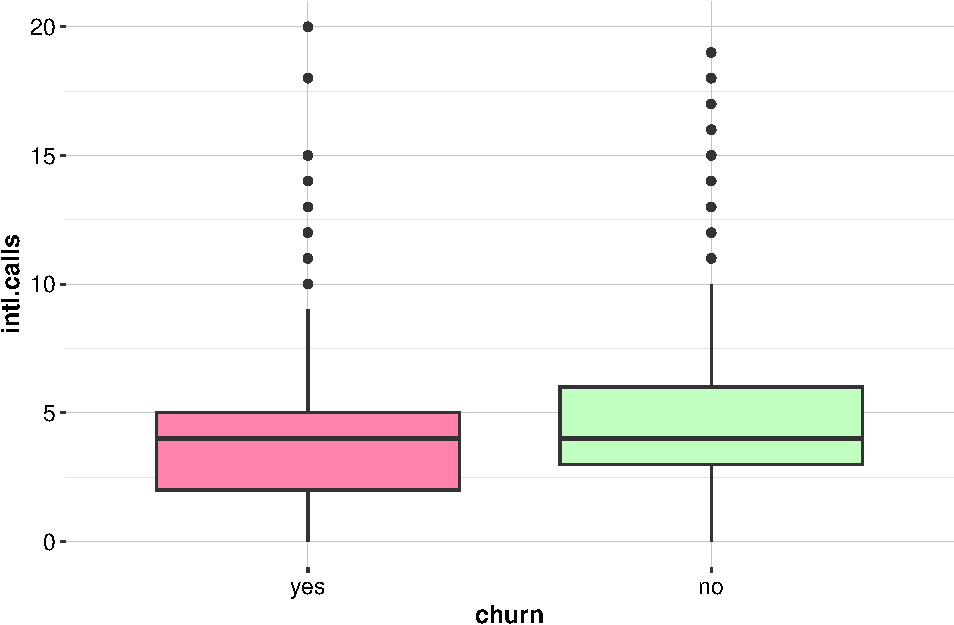
\includegraphics{statistics_files/figure-latex/unnamed-chunk-9-1} \end{center}

The boxplot compares the distribution of international calls for churners and non-churners. If the medians or spreads differ substantially, this may indicate that the variable has predictive importance. In this case, the plot does not reveal strong visual evidence of a difference, but to formally assess this, we proceed with the two-sample t-test.

To perform the test in \textbf{R}, we use the \passthrough{\lstinline!t.test()!} function:

\begin{lstlisting}[language=R]
t_test_calls <- t.test(intl.calls ~ churn, data = churn)
t_test_calls
   
    Welch Two Sample t-test
   
   data:  intl.calls by churn
   t = -3.2138, df = 931.13, p-value = 0.001355
   alternative hypothesis: true difference in means between group yes and group no is not equal to 0
   95 percent confidence interval:
    -0.5324872 -0.1287201
   sample estimates:
   mean in group yes  mean in group no 
            4.151344          4.481947
\end{lstlisting}

This function evaluates the difference in means between the two groups (\passthrough{\lstinline!churn = "yes"!} vs.~\passthrough{\lstinline!churn = "no"!}) and calculates a test statistic and corresponding p-value. Based on the output:

\begin{itemize}
\item
  The \textbf{p-value} = 0.0014. Since this value is less than the significance level (\(\alpha = 0.05\)), we \textbf{reject the null hypothesis (\(H_0\))}. This indicates that the mean number of international calls differs significantly between churners and non-churners.
\item
  The test also provides the \textbf{95\% confidence interval} = {[}-0.53, -0.13{]} for the difference in means. Since this interval does not include zero, it reinforces the conclusion that the difference is statistically significant. The confidence interval also quantifies the magnitude of the difference between the two groups.
\item
  Additionally, the \textbf{sample means} for the two groups are reported in the output:

  \begin{itemize}
  \tightlist
  \item
    Mean for churners = 4.15\\
  \item
    Mean for non-churners = 4.48
  \end{itemize}
\end{itemize}

These sample means allow us to directly compare the average number of international calls between churners and non-churners. For example, if churners made an average of 1.5 international calls while non-churners made 2.3 calls, this suggests that churners tend to make fewer international calls.

The two-sample t-test assumes that the two groups are independent, and that the numerical variable being compared (e.g., \passthrough{\lstinline!intl.calls!}) follows an approximately normal distribution within each group. While the test is robust to minor deviations from normality, these assumptions should always be checked, especially for small sample sizes.

From a practical standpoint, this result suggests that the number of international calls is a significant predictor of churn. Customers who churn tend to make fewer international calls on average. This insight can help businesses develop targeted strategies, such as offering discounts or improved international calling plans to customers who show low usage. Such interventions could potentially reduce churn rates by addressing factors associated with customer dissatisfaction.

Finally, it's worth noting that while this example uses a two-tailed test to detect any difference in means (higher or lower), one-tailed tests could be used if the research question specifies a directional hypothesis. For example, if the company specifically hypothesizes that churners make fewer international calls than non-churners, a one-tailed test could be performed to increase the test's sensitivity.

In summary, the two-sample t-test is a powerful and versatile tool for comparing group means and uncovering meaningful differences in data. By combining graphical exploration with statistical testing, we can make robust inferences and translate them into actionable business insights.

\subsection{Two-Sample Z-test}\label{two-sample-z-test}

The \textbf{two-sample Z-test} is used to compare the proportions of two groups to determine whether the observed difference in proportions is statistically significant. It is particularly useful for binary categorical variables, where the goal is to evaluate whether the proportions of success (or presence) in one group differ from those in another.

In the context of the \emph{churn} dataset, we can apply the two-sample Z-test to investigate whether there is a relationship between the target variable \emph{churn} and the variable \emph{Voice Mail Plan} (\passthrough{\lstinline!voice.plan!}). Specifically, we aim to test whether the proportion of churners who have a Voice Mail Plan differs from the proportion of non-churners with the plan.

First, let's visualize the relationship between \emph{Voice Mail Plan} and \emph{churn} using bar plots:

\begin{lstlisting}[language=R]
ggplot(data = churn) + 
  geom_bar(aes(x = voice.plan, fill = churn)) +
  scale_fill_manual(values = c("palevioletred1", "darkseagreen1")) 

ggplot(data = churn) + 
  geom_bar(aes(x = voice.plan, fill = churn), position = "fill") +
  scale_fill_manual(values = c("palevioletred1", "darkseagreen1")) 
\end{lstlisting}

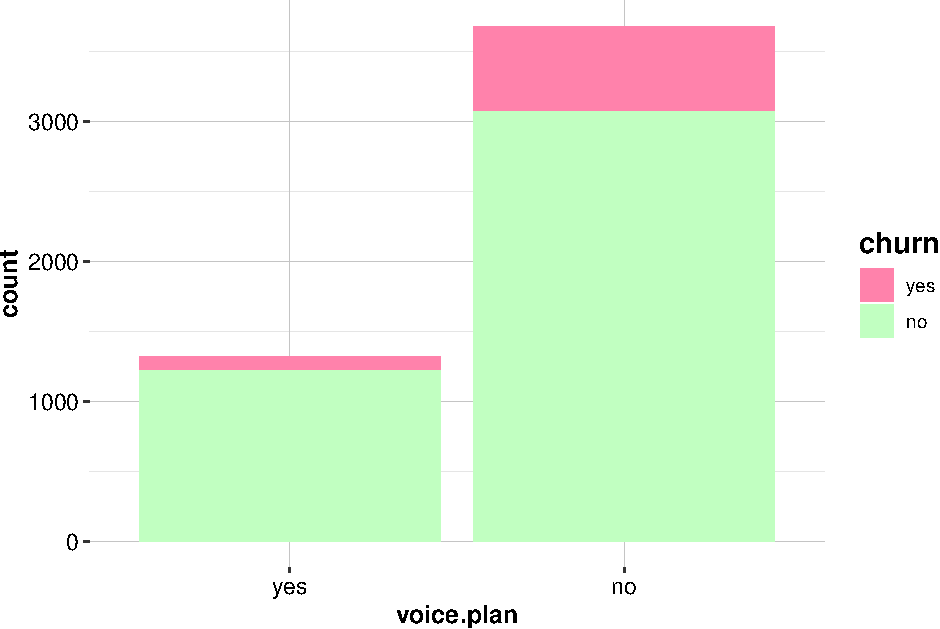
\includegraphics[width=0.5\linewidth]{statistics_files/figure-latex/unnamed-chunk-11-1} 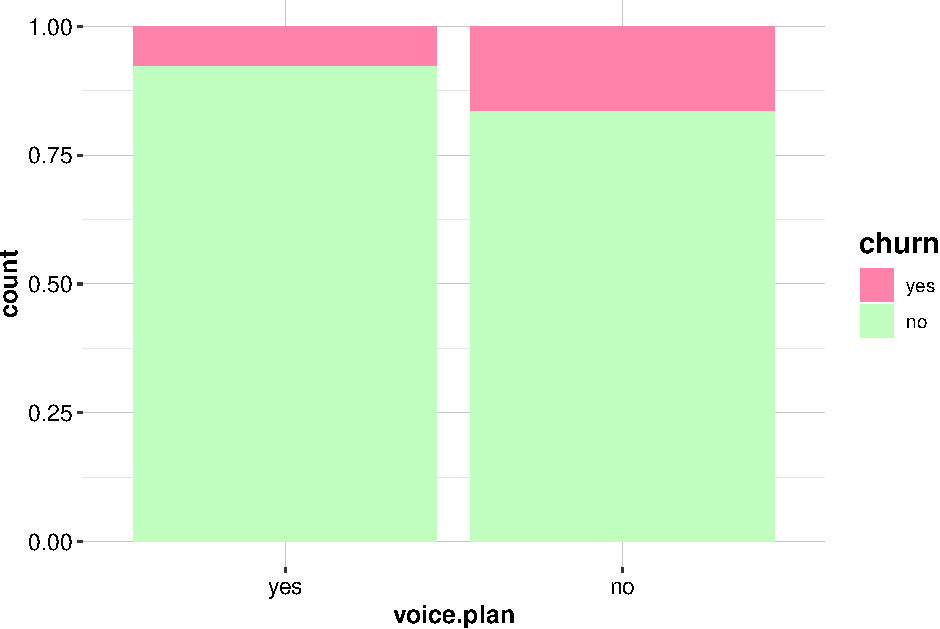
\includegraphics[width=0.5\linewidth]{statistics_files/figure-latex/unnamed-chunk-11-2}

The first bar plot shows the raw counts of churners and non-churners across the two categories of \emph{Voice Mail Plan} (Yes or No), while the second plot provides proportions, making it easier to compare the relative churn rates within each category. These visualizations suggest that the proportion of churners might differ based on whether they have a Voice Mail Plan, but a formal hypothesis test is needed to confirm this.

To test whether the proportions are significantly different, we set up the following hypotheses:

\begin{enumerate}
\def\labelenumi{\arabic{enumi}.}
\item
  \textbf{Null Hypothesis (\(H_0\))}: \(\pi_1 = \pi_2\)\\
  (The proportions of customers with a Voice Mail Plan are the same for churners and non-churners.)
\item
  \textbf{Alternative Hypothesis (\(H_a\))}: \(\pi_1 \neq \pi_2\)\\
  (The proportions of customers with a Voice Mail Plan differ between churners and non-churners.)
\end{enumerate}

These can also be expressed mathematically as:
\[
\bigg\{
\begin{matrix}
    H_0: \pi_1 = \pi_2   \\
    H_a: \pi_1 \neq \pi_2 
\end{matrix}
\]

To perform the Z-test in R, we first create a contingency table to summarize the counts of customers with and without a Voice Mail Plan in the churner and non-churner groups. This can be done using the \passthrough{\lstinline!table()!} function:

\begin{lstlisting}[language=R]
table_plan = table(churn$churn, churn$voice.plan, dnn = c("churn", "voice.plan"))
table_plan
        voice.plan
   churn  yes   no
     yes  102  605
     no  1221 3072
\end{lstlisting}

This table displays the count of customers for each combination of \emph{churn} and \emph{voice.plan}. For example, it might show how many churners and non-churners have subscribed to a Voice Mail Plan versus how many have not.

Next, we apply the \passthrough{\lstinline!prop.test()!} function to conduct the two-sample Z-test for the difference in proportions:

\begin{lstlisting}[language=R]
z_test = prop.test(table_plan)
z_test
   
    2-sample test for equality of proportions with continuity correction
   
   data:  table_plan
   X-squared = 60.552, df = 1, p-value = 7.165e-15
   alternative hypothesis: two.sided
   95 percent confidence interval:
    -0.1701734 -0.1101165
   sample estimates:
      prop 1    prop 2 
   0.1442716 0.2844165
\end{lstlisting}

The output of the test provides the \textbf{p-value}, the estimated proportions for each group, and the confidence interval for the difference in proportions. Based on the result:

\begin{itemize}
\item
  If the \textbf{p-value} (0) is less than the significance level (\(\alpha = 0.05\)), we reject the null hypothesis (\(H_0\)). This indicates that the difference in proportions is statistically significant, meaning the proportion of customers with a Voice Mail Plan differs between churners and non-churners.
\item
  The test also provides a \textbf{95\% confidence interval} = {[}-0.1702, -0.1101{]} for the difference in proportions. If this interval does not contain zero, it further confirms that the proportions are significantly different.
\end{itemize}

Additionally, the \textbf{sample proportions} for churners (0.1443) and non-churners (0.2844) are reported in the output. These represent the observed proportions of customers with a Voice Mail Plan in each group and allow for direct comparison.

Since the p-value is less than 0.05, we reject \(H_0\) and conclude that there is sufficient evidence to suggest that the proportion of Voice Mail Plan members differs between churners and non-churners. This result indicates that the variable \emph{Voice Mail Plan} is indeed useful for predicting churn.

From a business perspective, this insight suggests that customers without a Voice Mail Plan may be more likely to churn. Companies could leverage this information by promoting Voice Mail Plans to customers at risk of leaving or by investigating whether the feature is associated with improved customer satisfaction and retention.

In summary, the two-sample Z-test provides a formal method for comparing proportions between two groups. By combining visual exploration with hypothesis testing, we can identify significant relationships and use these findings to inform business strategies or further statistical modeling.

\subsection{Chi-square Test}\label{chi-square-test}

The \textbf{Chi-square test} is used to evaluate whether there is an association between two categorical variables. It assesses whether the observed frequencies in each category differ significantly from what would be expected under the assumption of independence. This test is particularly useful for variables with more than two categories, and it derives its name from the Chi-square (\(\chi^2\)) distribution on which it is based.

To illustrate, let's analyze whether there is a relationship between the variable \emph{marital} and the target variable \emph{deposit} in the \emph{bank} dataset (available in the \textbf{liver} package). The variable \passthrough{\lstinline!marital!} has three categories: ``divorced,'' ``married,'' and ``single,'' while the target variable \passthrough{\lstinline!deposit!} has two categories: ``yes'' (customers who purchased a deposit) and ``no'' (customers who did not). Our goal is to determine whether the marital status of customers is associated with their decision to make a deposit.

We start by visualizing the relationship between \passthrough{\lstinline!marital!} and \passthrough{\lstinline!deposit!} using bar plots:

\begin{lstlisting}[language=R]
ggplot(data = bank) + 
    geom_bar(aes(x = marital, fill = deposit)) +
    scale_fill_manual(values = c("palevioletred1", "darkseagreen1")) 

ggplot(data = bank) + 
    geom_bar(aes(x = marital, fill = deposit), position = "fill") +
    scale_fill_manual(values = c("palevioletred1", "darkseagreen1")) 
\end{lstlisting}

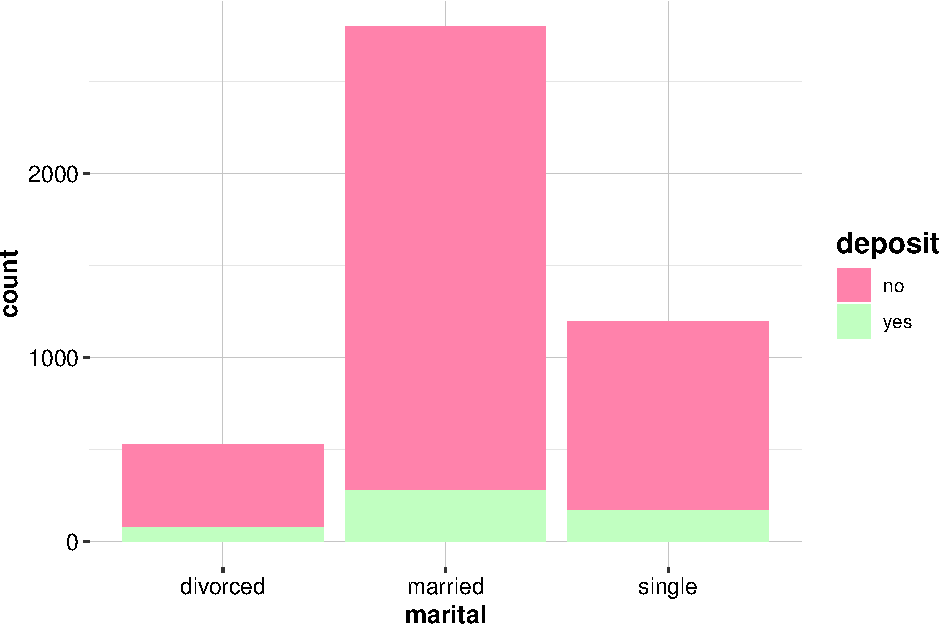
\includegraphics[width=0.5\linewidth]{statistics_files/figure-latex/unnamed-chunk-14-1} \includegraphics[width=0.5\linewidth]{statistics_files/figure-latex/unnamed-chunk-14-2}

The first bar plot shows the raw counts of deposits across marital categories, while the second plot shows the proportions within each marital group. These visualizations suggest that the marital status might influence the likelihood of making a deposit, but a formal hypothesis test is needed to confirm this.

We create a contingency table to summarize the counts of observations across the categories of \passthrough{\lstinline!marital!} and \passthrough{\lstinline!deposit!}:

\begin{lstlisting}[language=R]
table_marital <- table(bank$deposit, bank$marital, dnn = c("deposit", "marital"))
table_marital
          marital
   deposit divorced married single
       no       451    2520   1029
       yes       77     277    167
\end{lstlisting}

This table provides the observed frequencies of deposits (``yes'' and ``no'') across the marital categories. To test whether these proportions differ significantly, we use the Chi-square test with the following hypotheses:

\begin{enumerate}
\def\labelenumi{\arabic{enumi}.}
\tightlist
\item
  \textbf{Null Hypothesis (\(H_0\))}: The proportions of deposits are the same across all marital categories.\\
  Mathematically:\\
  \[
  \pi_{divorced, \ yes} = \pi_{married, \ yes} = \pi_{single, \ yes}
  \]
\item
  \textbf{Alternative Hypothesis (\(H_a\))}: At least one of the proportions differs from the others.
\end{enumerate}

The hypotheses can also be expressed as:
\[
\bigg\{
\begin{matrix}
    H_0: \text{Deposit rates are independent of marital status.} \\
    H_a: \text{Deposit rates depend on marital status.}
\end{matrix}
\]

We apply the Chi-square test using the \passthrough{\lstinline!chisq.test()!} function in R:

\begin{lstlisting}[language=R]
chisq_test <- chisq.test(table_marital)
chisq_test
   
    Pearson's Chi-squared test
   
   data:  table_marital
   X-squared = 19.03, df = 2, p-value = 7.374e-05
\end{lstlisting}

The output provides the Chi-square test statistic, degrees of freedom, and the \textbf{p-value}. Here, the \textbf{p-value} = \ensuremath{7.3735354\times 10^{-5}} is smaller than the significance level \(\alpha = 0.05\). Therefore, we reject the null hypothesis (\(H_0\)) and conclude that there is a statistically significant association between marital status and deposit behavior. In other words, the proportion of deposits differs across the marital categories.

Additionally, the output includes the expected frequencies under the null hypothesis, which can be compared with the observed frequencies to assess where the differences lie. These insights can guide further analysis, such as investigating which marital group contributes most to the association.

From a business perspective, this result indicates that marital status is a useful predictor of whether a customer will purchase a deposit. Marketing strategies can leverage this information by tailoring campaigns or offers to specific marital groups to increase deposit adoption rates.

In summary, the Chi-square test is a powerful tool for assessing relationships between categorical variables. By combining visualizations, contingency tables, and formal hypothesis testing, we can draw meaningful conclusions about the associations in our data and apply these insights to improve decision-making.

\subsection{Analysis of Variance (ANOVA) Test}\label{analysis-of-variance-anova-test}

The \textbf{Analysis of Variance (ANOVA)} test is used to compare the means of a numerical variable across more than two groups. It evaluates whether at least one group mean differs significantly from the others. ANOVA is especially useful when analyzing the relationship between a numerical variable and a categorical variable with multiple levels, providing a formal way to determine if the categorical variable impacts the numerical variable. The test relies on the F-distribution to assess whether the observed differences in means are statistically significant.

To illustrate, let's analyze the relationship between the variable \passthrough{\lstinline!cut!} and the target variable \passthrough{\lstinline!price!} in the popular \emph{diamonds} dataset (available in the \textbf{ggplot2} package). The variable \passthrough{\lstinline!cut!} has five categories (``Fair,'' ``Good,'' ``Very Good,'' ``Premium,'' and ``Ideal''), while \passthrough{\lstinline!price!} is numerical. Our objective is to test whether the mean price of diamonds differs across the five cut categories.

We begin with a box plot to visualize the distribution of diamond prices for each category of \passthrough{\lstinline!cut!}:

\begin{lstlisting}[language=R]
ggplot(data = diamonds) + 
  geom_boxplot(aes(x = cut, y = price, fill = cut)) +
  scale_fill_manual(values = c("palevioletred1", "darkseagreen1", "skyblue1", "gold1", "lightcoral"))
\end{lstlisting}

\begin{center}\includegraphics{statistics_files/figure-latex/unnamed-chunk-17-1} \end{center}

The box plot displays the spread and median prices for diamonds in each cut category. If the distributions appear distinct---for example, with noticeable differences in medians or ranges---this suggests that the cut might influence the price. However, visual inspection alone is insufficient to confirm whether these differences are statistically significant, so we proceed with an ANOVA test.

To formally test whether the mean prices differ by cut type, we set up the following hypotheses:

\begin{enumerate}
\def\labelenumi{\arabic{enumi}.}
\item
  \textbf{Null Hypothesis (\(H_0\))}: All group means are equal.\\
  Mathematically:\\
  \[
  \mu_1 = \mu_2 = \mu_3 = \mu_4 = \mu_5
  \]
  (The average prices are the same across all cut types.)
\item
  \textbf{Alternative Hypothesis (\(H_a\))}: At least one group mean is different.\\
  (Not all average prices are equal across the cut categories.)
\end{enumerate}

To conduct the ANOVA test in R, we use the \passthrough{\lstinline!aov()!} function as follows:

\begin{lstlisting}[language=R]
# Perform ANOVA
anova_test <- aov(price ~ cut, data = diamonds)
summary(anova_test)
                  Df    Sum Sq   Mean Sq F value Pr(>F)    
   cut             4 1.104e+10 2.760e+09   175.7 <2e-16 ***
   Residuals   53935 8.474e+11 1.571e+07                   
   ---
   Signif. codes:  0 '***' 0.001 '**' 0.01 '*' 0.05 '.' 0.1 ' ' 1
\end{lstlisting}

The output provides the test statistic (F-value), degrees of freedom, and the \textbf{p-value}. If the \textbf{p-value} is smaller than the significance level (\(\alpha = 0.05\)), we reject the null hypothesis (\(H_0\)). For instance, if the \textbf{p-value} = \ensuremath{8.4283073\times 10^{-150}}, we would reject \(H_0\) and conclude that not all group means are equal. This indicates that the variable \passthrough{\lstinline!cut!} has a significant impact on the price of diamonds.

It's important to note that rejecting \(H_0\) in ANOVA doesn't identify which specific groups differ. To determine this, we can conduct \textbf{post-hoc tests}, such as Tukey's Honestly Significant Difference (Tukey HSD) test, to pinpoint the pairs of categories that have significant differences in their means. In this example, we could apply Tukey's test to identify which cut categories (e.g., ``Ideal'' vs.~``Good'') drive the observed differences.

In summary, the ANOVA test confirms whether a categorical variable with multiple levels influences a numerical variable. In this case, the relationship between \passthrough{\lstinline!cut!} and \passthrough{\lstinline!price!} suggests that diamond cut type is an important predictor of price, providing valuable insight into how quality impacts cost.

\subsection{Correlation Test}\label{correlation-test}

The \textbf{correlation test} determines whether there is a significant linear relationship between two numerical variables by testing the null hypothesis that the population correlation coefficient (\(\rho\)) is equal to zero. This test evaluates both the direction and strength of the relationship between the variables.

In the diamonds dataset, let's explore whether there is a significant relationship between the variable \textbf{\passthrough{\lstinline!carat!}} (diamond weight) and the target variable \textbf{\passthrough{\lstinline!price!}} (diamond price). Visualizing the relationship between these two variables is often the first step in correlation analysis. Below is a scatter plot illustrating their relationship:

\begin{lstlisting}[language=R]
ggplot(data = diamonds) +
    geom_point(aes(x = carat, y = price), colour = "blue") +
    labs(x = "Carat", y = "Price") 
\end{lstlisting}

\begin{center}\includegraphics{statistics_files/figure-latex/unnamed-chunk-19-1} \end{center}

The scatter plot shows a clear upward trend, suggesting a positive relationship between \textbf{carat} and \textbf{price}---as the weight of the diamond increases, so does its price. To formally test whether this observed pattern is statistically significant, we establish the following hypotheses:

\begin{enumerate}
\def\labelenumi{\arabic{enumi}.}
\tightlist
\item
  \textbf{Null Hypothesis (\(H_0\))}: \(\rho = 0\) (There is no linear correlation between the variables.)
\item
  \textbf{Alternative Hypothesis (\(H_a\))}: \(\rho \neq 0\) (There is a significant linear correlation between the variables.)
\end{enumerate}

The hypotheses can be expressed as:
\[
\bigg\{
\begin{matrix}
    H_0: \rho   =  0 \\
    H_a: \rho \neq 0 
\end{matrix}
\]

To perform the correlation test in R, we use the \passthrough{\lstinline!cor.test()!} function:

\begin{lstlisting}[language=R]
cor_test <- cor.test(diamonds$carat, diamonds$price)
cor_test
   
    Pearson's product-moment correlation
   
   data:  diamonds$carat and diamonds$price
   t = 551.41, df = 53938, p-value < 2.2e-16
   alternative hypothesis: true correlation is not equal to 0
   95 percent confidence interval:
    0.9203098 0.9228530
   sample estimates:
         cor 
   0.9215913
\end{lstlisting}

The output of the correlation test includes the \textbf{p-value}, which quantifies the evidence against the null hypothesis. If the p-value = 0 is smaller than the significance level (\(\alpha = 0.05\)), we reject \(H_0\). In this case, the test result indicates strong evidence of a significant relationship between \textbf{\passthrough{\lstinline!carat!}} and \textbf{\passthrough{\lstinline!price!}}.

The test output also provides additional insights:

\begin{itemize}
\tightlist
\item
  \textbf{Correlation Coefficient}: The correlation coefficient (\(r = 0.92\)) measures the strength and direction of the relationship. A positive value near 1 indicates a strong positive correlation.
\item
  \textbf{95\% Confidence Interval}: The confidence interval {[}0.92, 0.92{]} provides a plausible range for the true population correlation (\(\rho\)). If this interval does not include 0, it reinforces the rejection of \(H_0\) and further confirms the presence of a significant correlation.
\end{itemize}

The correlation coefficient of 0.92 indicates a strong positive linear relationship between \textbf{\passthrough{\lstinline!carat!}} and \textbf{\passthrough{\lstinline!price!}}. Larger diamonds are associated with higher prices, which aligns with intuition and business practices in the diamond industry. The small p-value confirms that this relationship is statistically significant, not due to random chance. Furthermore, the confidence interval highlights the precision of our estimate for the population correlation, offering a range of plausible values for \(\rho\).

By combining visualization, hypothesis testing, and confidence intervals, we gain a comprehensive understanding of the relationship between \textbf{carat} and \textbf{price}, which can inform further analysis or predictive modeling.

\section{Wrapping Up}\label{wrapping-up}

In this chapter, we laid the foundation for statistical inference, starting with \textbf{estimation}, where we explored how point estimates and confidence intervals provide valuable insights into population parameters while accounting for uncertainty. We then turned to \textbf{hypothesis testing}, learning how to formulate null and alternative hypotheses, calculate test statistics, and interpret p-values to make data-driven decisions. Through practical examples, we applied a variety of techniques, such as the t-test for comparing means, tests for evaluating proportions, ANOVA for assessing group differences, and the Chi-square test and correlation analysis for uncovering relationships between variables. Together, these tools form a robust framework for answering research questions and drawing meaningful conclusions from data.

Statistical inference and hypothesis testing lie at the core of data analysis, offering a structured approach to distinguish meaningful patterns from random noise. These methods are indispensable for tasks like testing the effectiveness of a marketing strategy, evaluating the performance of a product, or predicting customer behavior. As you continue to apply these techniques, remember that the reliability of your results depends on \textbf{checking assumptions}, interpreting findings within the broader context of your data, and incorporating domain expertise to add depth to your conclusions.

In the next chapter, we'll build on these concepts as we prepare for machine learning by learning how to partition datasets effectively. To ensure that our partitions are valid and reliable, we will again rely on hypothesis testing. By connecting statistical inference to model-building, you'll see how the techniques from this chapter form the foundation for creating and validating predictive models.

\chapter{Preparing Data for Modeling}\label{chapter-modeling}

As we advance through the Data Science Process, illustrated in Chapter \ref{chapter-intro-DS}, Figure \ref{fig:CRISP-DM}, we've completed the foundational steps that pave the way for effective modeling:

\begin{enumerate}
\def\labelenumi{\arabic{enumi}.}
\tightlist
\item
  \textbf{Problem Understanding}: Chapter \ref{problem-understanding} highlighted the importance of clearly defining the problem and aligning objectives with data-driven strategies.\\
\item
  \textbf{Data Preparation}: In Chapter \ref{chapter-data-prep}, we addressed challenges such as missing values, outliers, and data transformation to ensure our dataset is clean and ready for analysis.\\
\item
  \textbf{Exploratory Data Analysis}: Chapter \ref{chapter-EDA} guided us through visualizing and summarizing data to uncover patterns and generate meaningful insights.\\
\item
  \textbf{Statistical Inference}: In Chapter \ref{chapter-statistics}, we explored hypothesis testing and feature selection, tools we'll leverage in this chapter to validate our data partitioning.
\end{enumerate}

Before diving into building machine learning models, it's essential to establish a robust foundation during what we'll refer to as the \textbf{Setup Phase}. This phase includes three critical tasks that must be completed before modeling begins:

\begin{itemize}
\tightlist
\item
  \textbf{Partitioning the Data}: Dividing the dataset into training and testing subsets to create a clear separation for model building and evaluation.\\
\item
  \textbf{Validating the Partition}: Ensuring the partition is appropriate and representative, allowing reliable insights to emerge from the training and testing process.\\
\item
  \textbf{Balancing the Training Dataset}: Addressing any imbalances in the training data (e.g., class imbalances in categorical targets) to ensure fair and accurate model training.
\end{itemize}

These tasks are often overlooked but play a crucial role in ensuring that the modeling process is both rigorous and effective.

When introducing this topic, students often ask, ``\emph{Why is it necessary to partition the data?}'' or ``\emph{Why do we need to follow these specific steps?}''. These are insightful questions---and ones we'll address in depth throughout this chapter. However, before diving into the details of partitioning and validating datasets, it's worth stepping back to examine how the Data Science Process aligns with and diverges from Statistical Inference. By understanding their similarities and differences, we can better appreciate the importance of these steps and how they bridge the principles of traditional statistics with the practical demands of modern machine learning.

\section{Statistical Inference in the Context of Data Science}\label{statistical-inference-in-the-context-of-data-science}

In Chapter \ref{chapter-statistics}, we explored how statistical inference helps us make conclusions about populations based on sample data. While this foundation remains valuable in the data science process, the goals and applications differ when preparing data for modeling.

Statistical inference and data science diverge in two key ways when applied to modeling tasks:

\begin{enumerate}
\def\labelenumi{\arabic{enumi}.}
\item
  \textbf{From Significance to Practicality}: In data science, where datasets often contain thousands or even millions of observations, nearly any difference or relationship becomes statistically significant. However, statistical significance does not necessarily equate to practical significance. For example, a machine learning model might identify a tiny effect size (e.g., a minor improvement in predictions) that is statistically significant but has no meaningful impact on decision-making. Thus, in modeling, the focus shifts to practical relevance and predictive power over mere statistical significance.
\item
  \textbf{Exploration vs.~Hypothesis Testing}: Traditional statistical inference begins with a specific hypothesis in mind, such as testing whether a new treatment improves outcomes compared to a control. In contrast, data science often takes an exploratory approach, using the data to uncover patterns, relationships, or actionable insights without a predefined hypothesis. For instance, in preparing data for modeling, we might investigate which features are most predictive of the target variable or assess relationships between variables to refine the dataset.
\end{enumerate}

That said, statistical inference still plays a critical role in the data science process, particularly in validating key steps during data preparation. For example:

\begin{itemize}
\tightlist
\item
  \textbf{Partition Validation}: When splitting the data into training and testing sets, statistical tests can confirm whether the two subsets are representative of the original dataset.
\item
  \textbf{Feature Selection}: Hypothesis tests can help identify which features have strong relationships with the target variable, aiding in selecting predictors for modeling.
\end{itemize}

By understanding these differences and leveraging statistical inference strategically, we can ensure that the data preparation process supports building robust, reliable, and interpretable models. As we proceed through this chapter, we'll see how inference and data science methods work together to create datasets that are both meaningful and ready for modeling.

\section{Why Is It Necessary to Partition the Data?}\label{why-is-it-necessary-to-partition-the-data}

Partitioning the dataset is a critical step in preparing data for modeling. A common question students ask when learning this topic is, ``\emph{Why do we need to partition the data?}''. The answer lies in the principle of \textbf{generalization}---the ability of a model to perform well on unseen data. Without proper partitioning, we risk building models that excel on the training data but fail to make accurate predictions in real-world scenarios. Partitioning ensures that a model's performance is evaluated on data it hasn't seen during training, providing an unbiased measure of its ability to generalize effectively.

The goal of partitioning is to divide the data into two distinct subsets: the \textbf{training set}, used to build the model, and the \textbf{testing set}, used to evaluate its performance. This separation simulates real-world conditions, where the model must make predictions on new, unseen data. Partitioning helps us detect and address common modeling pitfalls like \textbf{overfitting} and \textbf{underfitting}. These trade-offs are illustrated in Figure \ref{fig:model-complexity}, which highlights the balance between model complexity and performance on training and testing datasets.

\begin{figure}

{\centering \includegraphics[width=0.65\linewidth]{images/model_complexity} 

}

\caption{The trade-off between model complexity and accuracy on the training and test sets. It highlights the optimal model complexity (sweet spot), where the test set accuracy reaches its highest value for unseen data.}\label{fig:model-complexity}
\end{figure}

\textbf{Overfitting} occurs when a model learns the training data too well, including its noise and random fluctuations, instead of capturing the general patterns. Overfitted models achieve high accuracy on the training set but fail miserably on unseen data. For example, a churn prediction model might memorize customer IDs or irrelevant details instead of identifying meaningful behavioral trends. Such a model would struggle to predict churn for new customers and have little practical value.

\textbf{Underfitting}, on the other hand, arises when a model is too simplistic to capture the underlying patterns in the data. This might happen if the model lacks complexity or if preprocessing removes too much useful information. Underfitted models perform poorly on both the training and testing sets, failing to capture the signal within the data. For instance, a churn model that predicts the overall churn rate for all customers, without considering individual characteristics, would lack predictive power.

Partitioning addresses these issues by enabling us to evaluate the model's performance on unseen data (the testing set). By comparing accuracy on the training and testing sets, we can identify whether the model is overfitting (high training accuracy but low testing accuracy) or underfitting (low accuracy on both datasets). This evaluation helps us iteratively refine the model and strike the right balance between complexity and generalization.

Partitioning also protects against \textbf{data leakage}, a critical issue where information from the testing set inadvertently influences the training process. Data leakage inflates performance metrics, leading to a false sense of confidence in the model's abilities. By strictly separating the testing set from the training process, we can obtain a more realistic and reliable assessment of the model's generalization performance.

Beyond simple train-test splits, \textbf{cross-validation} is a powerful technique that improves the robustness of partitioning. In cross-validation, the dataset is divided into multiple subsets, or ``folds.'' The model is trained on a subset of the data and tested on a different fold, with this process repeated across all folds. The results are averaged to provide a more reliable estimate of model performance. Cross-validation is particularly useful when working with smaller datasets or when tuning hyperparameters, as it minimizes bias and variance introduced by a single train-test split.

Partitioning the data isn't just a procedural step---it's a cornerstone of building models that perform well in real-world applications. By systematically addressing overfitting, underfitting, and data leakage, and by incorporating techniques like cross-validation, we ensure that the model is not only well-suited to the training data but also capable of making accurate predictions on unseen data.

To summarize, the general strategy for supervised machine learning models consists of three key steps, illustrated in Figure \ref{fig:modeling}:

\begin{enumerate}
\def\labelenumi{\arabic{enumi}.}
\tightlist
\item
  \textbf{Partitioning} the dataset into training and testing sets, followed by validating the partition.\\
\item
  \textbf{Building} machine learning models on the training data.\\
\item
  \textbf{Evaluating} the performance of the models on the testing data to identify the most effective approach.
\end{enumerate}

\begin{figure}

{\centering \includegraphics[width=0.8\linewidth]{images/partitioning} 

}

\caption{A general predictive machine learning process for building and evaluating models. The 80-20 split ratio is an example and may vary based on the dataset and task.}\label{fig:modeling}
\end{figure}

By following this process, we create models that are both reliable and capable of generalizing to unseen data. In this chapter, we will focus on the crucial first step: partitioning the data effectively, validating the partition, and preparing a balanced training dataset. These steps form the foundation for robust model building and evaluation, paving the way for impactful, data-driven decision-making.

\section{Partitioning the Data}\label{sec-partitioning}

Partitioning data is a crucial step in preparing it for machine learning. The most common method is the \textbf{train-test split}, also known as the holdout method, where the dataset is divided into two subsets: the training set and the testing set (Figure \ref{fig:modeling}). The training set is used to build the model, while the testing set is reserved for evaluating its performance. The split ratio is typically 70-30, 80-20, or 90-10, depending on the dataset size and the specific modeling task.

In this process, the training set includes all records with complete information, including the target variable. The testing set, however, has the target variable temporarily hidden to simulate unseen data. Machine learning models are trained exclusively on the training set, learning patterns and trends. These models are then applied to the test set to predict the hidden target values. Finally, the predictions are compared to the actual (restored) target values in the test set to evaluate the model's performance. This approach ensures the model is evaluated on unseen data, providing an unbiased measure of its generalization ability. Cross-validation further safeguards against overfitting by minimizing the chance of random variations being present in both sets.

For example, consider the \emph{churn} dataset, where the goal is to predict customer churn based on various features, as we'll explore in Chapter \ref{chapter-knn}. In this case, the train-test split divides the data into two subsets:
- The \textbf{training set}, which includes customer features and their known churn status.\\
- The \textbf{testing set}, which includes customer features but omits the churn status (temporarily treated as unknown).

In R, the \textbf{liver} package offers the \passthrough{\lstinline!partition()!} function for creating a train-test split. Here's how the \emph{churn} dataset can be split into training and testing sets:

\begin{lstlisting}[language=R]
set.seed(43)

data_sets = partition(data = churn, ratio = c(0.8, 0.2))

train_set = data_sets$part1
test_set  = data_sets$part2

actual_test  = test_set$deposit
\end{lstlisting}

In this example:

\begin{enumerate}
\def\labelenumi{\arabic{enumi}.}
\tightlist
\item
  \textbf{\passthrough{\lstinline!set.seed(43)!}}: Sets a seed to ensure reproducibility, so the split remains consistent across runs.\\
\item
  \textbf{\passthrough{\lstinline!partition()!}}: Splits the dataset into 80\% training data (\passthrough{\lstinline!train\_set!}) and 20\% testing data (\passthrough{\lstinline!test\_set!}).\\
\item
  \textbf{\passthrough{\lstinline!actual\_test!}}: Stores the true target values from the testing set for later evaluation.
\end{enumerate}

Reproducibility is essential in data science. By setting a seed, you ensure that the random split can be recreated exactly, allowing others to replicate your results or grade assignments reliably. Any integer can be used as the seed value---it doesn't need to match the one used here. Setting a seed is a best practice, particularly when sharing code or collaborating with others, as it eliminates inconsistencies and ensures precise reproducibility.

By applying a train-test split, we establish a reliable framework for evaluating model performance and ensure the robustness of our results. In the next steps, this foundation will allow us to validate partitions, balance training datasets, and build effective machine learning models.

\section{Validating the Partition}\label{sec-validate-partition}

The success of the entire modeling process depends on the quality of the data partition. Validating the partition ensures that both the training and testing sets are representative of the original dataset, enabling the model to learn from diverse examples and generalize effectively to unseen data. Without validation, the modeling process risks bias---either the model fails to generalize because the training set isn't representative, or the testing set doesn't provide an accurate evaluation of real-world performance.

Validation involves comparing the training and testing sets to confirm that their distributions are statistically similar, particularly for key variables. Since datasets often include many variables, this step typically focuses on a small set of randomly selected features or features of particular importance, such as the target variable. The choice of statistical test depends on the type of variable being compared, as shown in Table \ref{tab:partition-test}.

\begin{longtable}[]{@{}
  >{\raggedright\arraybackslash}p{(\linewidth - 2\tabcolsep) * \real{0.4300}}
  >{\raggedright\arraybackslash}p{(\linewidth - 2\tabcolsep) * \real{0.5700}}@{}}
\caption{\label{tab:partition-test} Suggested hypothesis tests for validating partitions, based on the type of target variable.}\tabularnewline
\toprule\noalign{}
\begin{minipage}[b]{\linewidth}\raggedright
Type of Variable
\end{minipage} & \begin{minipage}[b]{\linewidth}\raggedright
Suggested Test (from Chapter \ref{chapter-statistics})
\end{minipage} \\
\midrule\noalign{}
\endfirsthead
\toprule\noalign{}
\begin{minipage}[b]{\linewidth}\raggedright
Type of Variable
\end{minipage} & \begin{minipage}[b]{\linewidth}\raggedright
Suggested Test (from Chapter \ref{chapter-statistics})
\end{minipage} \\
\midrule\noalign{}
\endhead
\bottomrule\noalign{}
\endlastfoot
Numerical variable & Two-sample t-test \\
Binary/Flag variable & Two-sample Z-test \\
Categorical variable (with \textgreater{} 2 categories) & Chi-square test \\
\end{longtable}

Validating the partition is more than a procedural step---it is a safeguard against biased modeling. If the training and testing sets differ significantly, the model's performance could be compromised. For example, if the training set isn't representative of the original dataset, the model may fail to generalize. Conversely, if the testing set isn't representative, the evaluation results may be overly optimistic. Ensuring that the split reflects the original dataset's characteristics allows for fair and reliable model evaluation.

\begin{example}
\protect\hypertarget{exm:ex-test-partition}{}\label{exm:ex-test-partition}Let's consider the \emph{churn} dataset introduced in the previous section. The target variable, \emph{churn} (whether a customer has churned or not), is binary. According to Table \ref{tab:partition-test}, the appropriate statistical test to validate the partition for this variable is a \textbf{Two-Sample Z-Test}, which compares the proportion of churned customers in the training and testing sets. Here's how it can be implemented in R:

\begin{lstlisting}[language=R]
x1 <- sum(train_set$churn == "yes")
x2 <- sum(test_set$churn == "yes")

n1 <- nrow(train_set)
n2 <- nrow(test_set)

test_churn <- prop.test(x = c(x1, x2), n = c(n1, n2))
test_churn
   
    2-sample test for equality of proportions with continuity correction
   
   data:  c(x1, x2) out of c(n1, n2)
   X-squared = 0.1566, df = 1, p-value = 0.6923
   alternative hypothesis: two.sided
   95 percent confidence interval:
    -0.0190317  0.0300317
   sample estimates:
   prop 1 prop 2 
   0.1425 0.1370
\end{lstlisting}

In this example:

\begin{itemize}
\tightlist
\item
  \(x_1\) and \(x_2\) represent the number of churned customers in the training and testing sets, respectively.\\
\item
  \(n_1\) and \(n_2\) represent the total number of observations in the training and testing sets, respectively.\\
\item
  The \passthrough{\lstinline!prop.test()!} function compares the proportions of churned customers between the two subsets.
\end{itemize}

The hypotheses for the test are:\\
\[
\bigg\{
\begin{matrix}
H_0:  \pi_{\text{churn, train}} = \pi_{\text{churn, test}} \quad \text{(Proportions are equal)} \\
H_a:  \pi_{\text{churn, train}} \neq \pi_{\text{churn, test}} \quad \text{(Proportions are not equal)}
\end{matrix}
\]

The test result provides a \emph{p}-value = 0.69. Since the \emph{p}-value is greater than the significance level (\(\alpha = 0.05\)), we fail to reject the null hypothesis (\(H_0\)). This indicates no statistically significant difference in the proportions of churned customers between the training and testing sets. By failing to reject \(H_0\), we confirm that the partition is valid with respect to the target variable \emph{churn}. The proportions of churned customers are consistent across both subsets, ensuring that the model will be trained and tested on representative data.
\end{example}

Beyond validating the target variable, you can extend this process to other key features in the dataset. For example, you might compare numerical features like \passthrough{\lstinline!customer.calls!} or \passthrough{\lstinline!day.mins!} using a two-sample t-test or validate categorical features with more than two categories using a Chi-square test. This broader validation ensures that the partition is representative across all relevant variables.

\emph{What If the Partition Is Invalid?} For example, if significant differences are found between the training and testing sets---several corrective actions can be taken. You could revisit the partitioning process by changing the random seed, adjusting the split ratio, or using stratified sampling to ensure that key features are proportionally represented in both subsets. Alternatively, techniques like k-fold cross-validation can provide a more robust approach by using all observations for both training and testing across multiple iterations.

Validating the partition is a critical step in the data preparation process. It ensures that the modeling process is fair, reliable, and capable of producing generalizable results. By addressing potential discrepancies early, we set the stage for robust machine learning models that perform effectively on real-world, unseen data.

\section{Balancing the Training Dataset}\label{balancing-the-training-dataset}

In some real-world classification problems, one class of the target variable is often significantly underrepresented compared to the other(s). This imbalance can lead to biased models that perform well for the majority class but poorly for the minority class. For example, in a fraud detection dataset, fraudulent transactions may account for only a tiny fraction of the data, while legitimate transactions dominate. Similarly, in a churn prediction dataset, the majority of customers might not churn, while only a small percentage do. If left unaddressed, this imbalance can result in models that fail to accurately predict the minority class, despite appearing to perform well overall.

Imbalanced datasets are problematic because most machine learning algorithms optimize for overall accuracy, which can favor the majority class. A model trained on an imbalanced churn dataset, for example, might predict ``no churn'' for almost all customers, resulting in high accuracy but completely missing the minority class of customers likely to churn. This failure can have significant implications, particularly in cases where the minority class---such as fraud cases, churners, or patients with a rare disease---is of critical importance.

To address this issue, balancing the training dataset ensures that both classes are adequately represented during model training. By exposing the model to sufficient examples from the minority class, balancing helps the model learn patterns and trends from both classes, improving its ability to generalize and make accurate predictions for the minority class. Common techniques for balancing include:

\begin{enumerate}
\def\labelenumi{\arabic{enumi}.}
\tightlist
\item
  \textbf{Oversampling}: Increasing the number of minority class examples by duplicating existing observations or generating synthetic samples (e.g., using SMOTE).\\
\item
  \textbf{Undersampling}: Reducing the number of majority class examples by randomly removing observations.\\
\item
  \textbf{Hybrid Methods}: Combining oversampling and undersampling to achieve a balanced dataset.\\
\item
  \textbf{Class Weights}: Modifying the algorithm to penalize misclassifications of the minority class more heavily during training.
\end{enumerate}

The choice of technique depends on factors such as the dataset size, the degree of imbalance, and the specific machine learning algorithm being used. Let's demonstrate balancing the training dataset with an example using the churn dataset.

First, we examine the distribution of the target variable, \emph{churn}, in the training dataset to determine whether balancing is necessary. This can be done in R as follows:

\begin{lstlisting}[language=R]
# Check the class distribution
table(train_set$churn)
   
    yes   no 
    570 3430
prop.table(table(train_set$churn))
   
      yes     no 
   0.1425 0.8575
\end{lstlisting}

Suppose the output reveals that the proportion of customers who churn (\passthrough{\lstinline!churn = "yes"!}) is only 0.14 while the proportion of non-churners (\passthrough{\lstinline!churn = "no"!}) is 0.86. This significant imbalance suggests that balancing may be beneficial, particularly if predicting churners is a priority.

To balance the training dataset, we use the \textbf{ROSE} package in R to oversample the minority class (\passthrough{\lstinline!churn = "yes"!}) so that it constitutes 30\% of the training dataset. Here's how this can be implemented:

\begin{lstlisting}[language=R]
# Load the ROSE package
library(ROSE)

# Oversample the training set to balance the classes with 30% churners
balanced_train_set <- ovun.sample(churn ~ ., data = train_set, method = "over", 
                                  p = 0.3)$data

# Check the new class distribution
table(balanced_train_set$churn)
   
     no  yes 
   3430 1444
prop.table(table(balanced_train_set$churn))
   
          no       yes 
   0.7037341 0.2962659
\end{lstlisting}

In this example, the \passthrough{\lstinline!ovun.sample()!} function is used to oversample the minority class, achieving the desired class distribution. The parameter \passthrough{\lstinline!p = 0.3!} specifies that churners should comprise 30\% of the balanced training dataset. Notably, the formula notation \passthrough{\lstinline!churn \~ .!} indicates that the balancing is performed based on the target variable \passthrough{\lstinline!churn!} (refer to Section \ref{sec-formula-in-R} for details on formula notation). After oversampling, the new class distribution is examined to ensure that the dataset reflects the specified proportions.

Balancing ensures that the model is exposed to a sufficient number of examples from both churners and non-churners during training. For instance, a decision tree trained on this balanced dataset would give equal importance to features predictive of churn, rather than being dominated by the majority class.

It's important to note that balancing should be applied only to the \textbf{training dataset}, not the test dataset. The test dataset should remain representative of the original data distribution to provide an unbiased evaluation of the model's generalization performance. Balancing the test set can introduce bias and lead to overly optimistic performance metrics, which do not reflect real-world conditions.

Moreover, balancing must be performed \textbf{after partitioning} the dataset into training and testing sets. Balancing before partitioning can lead to \textbf{data leakage}, where information from the test set influences the training process. This compromises the integrity of the modeling process and inflates performance metrics, creating a false sense of confidence in the model's ability to generalize.

That said, balancing is not always necessary. Many modern machine learning algorithms, such as random forests and gradient boosting machines, are robust to class imbalances and incorporate techniques like class weighting to handle minority classes effectively. Additionally, evaluation metrics such as precision, recall, F1-score, and AUC-ROC are designed to account for class imbalance, providing a fairer assessment of model performance even when the dataset remains imbalanced.

In summary, balancing the training dataset can address class imbalance, especially when the minority class is critical to the analysis. However, it is not always required and should be used judiciously. If balancing is deemed necessary, it must be performed on the training dataset \textbf{after partitioning} to maintain the validity and reliability of the modeling process. By carefully balancing the training data, we ensure that models are better equipped to handle the minority class, resulting in fairer and more effective predictions.

\chapter{Classification using k-Nearest Neighbors}\label{chapter-knn}

The k-Nearest Neighbors (kNN) algorithm is a simple yet effective machine learning technique, widely used for solving classification problems. Its intuitive approach and ease of implementation make it a go-to choice for beginners and a reliable tool for experienced practitioners. In this chapter, we will delve into the details of the kNN algorithm, demonstrate its implementation in R, and discuss its practical applications. But before we focus on kNN, it's essential to revisit the fundamental concept of classification, one of the cornerstone tasks in machine learning.

\section{Classification}\label{classification}

Have you ever wondered how your email app effortlessly filters spam, how your streaming service seems to know exactly what you want to watch next, or how banks detect fraudulent credit card transactions in real-time? These seemingly magical predictions are made possible by \textbf{classification}, a fundamental task in machine learning.

At its core, classification involves assigning a label or category to an observation based on its features. For example, given customer data, classification can predict whether they are likely to churn or stay loyal. Unlike regression, which predicts continuous numerical values (e.g., house prices), classification deals with discrete outcomes. The target variable, often called the \textbf{class} or \textbf{label}, can either be:

\begin{itemize}
\tightlist
\item
  \textbf{Binary}: Two possible categories (e.g., spam vs.~not spam).\\
\item
  \textbf{Multi-class}: More than two categories (e.g., car, bicycle, or pedestrian in image recognition).
\end{itemize}

From diagnosing diseases to identifying fraudulent activities, classification is a versatile tool used across countless domains to solve practical problems.

\subsection*{Where Is Classification Used?}\label{where-is-classification-used}
\addcontentsline{toc}{subsection}{Where Is Classification Used?}

Classification algorithms power many everyday applications and cutting-edge technologies. Here are some examples:\\
- \textbf{Email filtering}: Sorting spam from non-spam messages.\\
- \textbf{Fraud detection}: Identifying suspicious credit card transactions.\\
- \textbf{Customer retention}: Predicting whether a customer will churn.\\
- \textbf{Medical diagnosis}: Diagnosing diseases based on patient records.\\
- \textbf{Object recognition}: Detecting pedestrians and vehicles in self-driving cars.\\
- \textbf{Recommendation systems}: Suggesting movies, songs, or products based on user preferences.

Every time you interact with technology that ``predicts'' something for you, chances are, a classification model is working behind the scenes.

\subsection*{How Does Classification Work?}\label{how-does-classification-work}
\addcontentsline{toc}{subsection}{How Does Classification Work?}

Classification involves two critical phases:

\begin{enumerate}
\def\labelenumi{\arabic{enumi}.}
\tightlist
\item
  \textbf{Training Phase}: The algorithm learns patterns from a labeled dataset, which contains both predictor variables (features) and target class labels. For instance, in a fraud detection system, the algorithm might learn that transactions involving unusually high amounts and originating from foreign locations are more likely to be fraudulent.\\
\item
  \textbf{Prediction Phase}: Once the model is trained, it applies these learned patterns to classify new, unseen data. For example, given a new transaction, the model predicts whether it is fraudulent or legitimate.
\end{enumerate}

A good classification model does more than just memorize the training data---it \textbf{generalizes} well, meaning it performs accurately on new, unseen data. For example, a model trained on historical medical data should be able to correctly diagnose a new patient it has never seen before.

\subsection*{Which Classification Algorithm Should You Use?}\label{which-classification-algorithm-should-you-use}
\addcontentsline{toc}{subsection}{Which Classification Algorithm Should You Use?}

Different classification algorithms are designed for different kinds of problems and datasets. Some commonly used algorithms include:\\
- \textbf{k-Nearest Neighbors (kNN)}: A simple, distance-based algorithm (covered in this chapter).\\
- \textbf{Logistic Regression}: Popular for binary classification tasks, such as predicting customer churn.\\
- \textbf{Decision Trees and Random Forests}: Versatile, interpretable methods for complex problems.\\
- \textbf{Naive Bayes}: Particularly useful for text classification, like spam filtering.\\
- \textbf{Neural Networks}: Effective for handling high-dimensional and complex data, such as images or natural language.

The choice of algorithm depends on factors like the dataset size, feature relationships, and the desired trade-off between interpretability and performance. For example, if you're working with a small dataset and need an easy-to-interpret solution, kNN or Decision Trees might be ideal. On the other hand, if you're analyzing high-dimensional data like images, Neural Networks could be more suitable.

To see classification in action, imagine a \textbf{bank dataset} where the goal is to predict whether a customer will make a deposit (\passthrough{\lstinline!deposit = yes!}) or not (\passthrough{\lstinline!deposit = no!}). The features might include customer details like \passthrough{\lstinline!age!}, \passthrough{\lstinline!education!}, \passthrough{\lstinline!job!}, and \passthrough{\lstinline!marital status!}. By training a classification model on this data, the bank can identify and target potential customers who are likely to invest, improving their marketing strategy.

\subsection*{Why Is Classification Important?}\label{why-is-classification-important}
\addcontentsline{toc}{subsection}{Why Is Classification Important?}

Classification forms the backbone of countless machine learning applications that drive smarter decisions and actionable insights in industries like finance, healthcare, retail, and technology. Understanding how it works is a critical step in mastering machine learning and applying it to solve real-world problems.

In the rest of this chapter, we'll explore the \textbf{k-Nearest Neighbors (kNN)} algorithm, a straightforward yet powerful method for classification. Its simplicity and intuitive nature make it an excellent choice for beginners and a foundational building block for more advanced algorithms. Let's dive in!

\section{How k-Nearest Neighbors Works}\label{how-k-nearest-neighbors-works}

Have you ever tried to make a decision by asking a few trusted friends for their advice? The \textbf{k-Nearest Neighbors (kNN)} algorithm works in a similar way---it ``asks'' the nearest data points in its neighborhood to determine the category of a new observation. This simple yet powerful idea makes kNN one of the most intuitive methods in machine learning.

Unlike many algorithms that require a complex training phase, kNN is a \textbf{lazy learning} or \textbf{instance-based} method. It doesn't build an explicit model during training; instead, it stores the entire training dataset and makes predictions on-the-fly by finding the nearest neighbors of a given observation. The parameter \(k\) determines how many neighbors to consider, and the majority class among these neighbors becomes the prediction.

\subsection*{How Does kNN Classify a New Observation?}\label{how-does-knn-classify-a-new-observation}
\addcontentsline{toc}{subsection}{How Does kNN Classify a New Observation?}

When a new observation needs to be classified, kNN calculates its \textbf{distance} to every data point in the training set using a specified distance metric, such as Euclidean distance. The algorithm identifies the \(k\)-nearest neighbors and predicts the class based on a \textbf{majority vote} among these neighbors.

To better understand how this works, let's look at Figure \ref{fig:knn-image}, which illustrates a simple example with two classes: {Class A (red circles)} and {Class B (blue squares)}.

A new data point, represented by a \textbf{dark star}, needs to be classified. The figure demonstrates the predictions for two different values of \(k\):

\begin{enumerate}
\def\labelenumi{\arabic{enumi}.}
\tightlist
\item
  \textbf{When \(k = 3\)}: The algorithm looks at the 3 closest neighbors to the dark star---two blue squares and one red circle. Since the majority of these neighbors belong to \textbf{Class B (blue squares)}, the new point is classified as Class B.\\
\item
  \textbf{When \(k = 6\)}: The algorithm now considers a larger neighborhood of 6 neighbors. In this case, four red circles and two blue squares are the nearest neighbors. With the majority vote shifting to \textbf{Class A (red circles)}, the new point is classified as Class A.
\end{enumerate}

\begin{figure}

{\centering \includegraphics[width=0.75\linewidth]{images/knn} 

}

\caption{A two-dimensional toy dataset with two classes (Class A and Class B) and a new data point (dark star), illustrating the k-Nearest Neighbors algorithm with k = 3 and k = 6.}\label{fig:knn-image}
\end{figure}

\textbf{Key Takeaway from the Figure:}

\begin{itemize}
\tightlist
\item
  Increasing \(k\) smooths predictions by incorporating more neighbors into the decision-making process. However, this may lead to less sensitivity to local patterns.\\
\item
  In this example, when \(k = 6\), the larger neighborhood includes more red circles, shifting the majority class to Class A. This demonstrates how majority voting in larger neighborhoods can significantly affect the outcome.
\end{itemize}

\subsection*{Strengths and Limitations of kNN}\label{strengths-and-limitations-of-knn}
\addcontentsline{toc}{subsection}{Strengths and Limitations of kNN}

The simplicity of kNN makes it an excellent starting point for understanding classification. By relying only on distance metrics and majority voting, it avoids the complexity of training explicit models. However, this simplicity comes with trade-offs:

\begin{itemize}
\tightlist
\item
  \textbf{Strengths}:

  \begin{itemize}
  \tightlist
  \item
    Easy to understand and implement.\\
  \item
    Effective for small datasets with clear patterns.
  \end{itemize}
\item
  \textbf{Limitations}:

  \begin{itemize}
  \tightlist
  \item
    Sensitive to irrelevant or noisy features, as distance calculations may become less meaningful.\\
  \item
    Computationally expensive for large datasets, since the algorithm must compute distances for all training points during prediction.\\
  \item
    Requires careful choice of \(k\) to balance sensitivity to local patterns and robustness to noise.
  \end{itemize}
\end{itemize}

\subsection*{A Practical Example of kNN in Action}\label{a-practical-example-of-knn-in-action}
\addcontentsline{toc}{subsection}{A Practical Example of kNN in Action}

To further illustrate kNN, consider a toy simulated example from a real-world scenario involving drug prescription classification. A dataset of 200 patients includes their \textbf{age}, \textbf{sodium-to-potassium (Na/K) ratio}, and the drug type they were prescribed. Figure \ref{fig:scatter-plot-ex-drug} shows a scatter plot of this data, where the drug types are represented by:

\begin{itemize}
\tightlist
\item
  \textbf{Red circles} for Drug A,\\
\item
  \textbf{Green triangles} for Drug B, and\\
\item
  \textbf{Blue squares} for Drug C.
\end{itemize}

\begin{figure}

{\centering \includegraphics[width=0.85\linewidth]{knn_files/figure-latex/scatter-plot-ex-drug-1} 

}

\caption{Scatter plot of Age vs. Sodium/Potassium Ratio for 200 patients, with drug type indicated by color and shape.}\label{fig:scatter-plot-ex-drug}
\end{figure}

Suppose we now have three new patients whose drug classifications are unknown. Their details are as follows:

\begin{enumerate}
\def\labelenumi{\arabic{enumi}.}
\tightlist
\item
  \textbf{Patient 1}: 40 years old with a Na/K ratio of 30.5,\\
\item
  \textbf{Patient 2}: 28 years old with a Na/K ratio of 9.6, and\\
\item
  \textbf{Patient 3}: 61 years old with a Na/K ratio of 10.5.
\end{enumerate}

These patients are represented as \textbf{orange circles} in Figure \ref{fig:scatter-plot-ex-drug-2}. Using kNN, we will classify the drug type for each patient.

\begin{figure}

{\centering \includegraphics[width=0.85\linewidth]{knn_files/figure-latex/scatter-plot-ex-drug-2-1} 

}

\caption{Scatter plot of Age vs. Sodium/Potassium Ratio for 200 patients, with drug type indicated by color and shape. The three new patients are represented by large orange circles.}\label{fig:scatter-plot-ex-drug-2}
\end{figure}

For \textbf{Patient 1}, who is located deep within a cluster of red-circle points (Drug A), the classification is straightforward: \textbf{Drug A}. All the nearest neighbors belong to Drug A, making it an easy decision.

For \textbf{Patient 2}, the situation is more nuanced.

\begin{itemize}
\tightlist
\item
  \textbf{With \(k = 1\)}: The nearest neighbor is a blue square, so the classification is \textbf{Drug C}.\\
\item
  \textbf{With \(k = 2\)}: There is a tie between Drug B and Drug C, leaving no clear majority.\\
\item
  \textbf{With \(k = 3\)}: Two out of the three nearest neighbors are blue squares, resulting in a majority vote for \textbf{Drug C}.
\end{itemize}

For \textbf{Patient 3}, the scenario becomes even more ambiguous:

\begin{itemize}
\tightlist
\item
  \textbf{With \(k = 1\)}: The closest neighbor is a blue square, so the classification is \textbf{Drug C}.\\
\item
  \textbf{With \(k = 2 or 3\)}: The neighbors belong to multiple classes, resulting in ties or uncertainty.
\end{itemize}

\begin{figure}
\includegraphics[width=0.33\linewidth]{knn_files/figure-latex/scatter-plot-ex-drug-3-1} \includegraphics[width=0.33\linewidth]{knn_files/figure-latex/scatter-plot-ex-drug-3-2} \includegraphics[width=0.33\linewidth]{knn_files/figure-latex/scatter-plot-ex-drug-3-3} \caption{Zoom-in plots for the three new patients and their nearest neighbors. The left plot is for Patient 1, the middle plot is for Patient 2, and the right plot is for Patient 3.}\label{fig:scatter-plot-ex-drug-3}
\end{figure}

These examples illustrate several key considerations for kNN:

\begin{itemize}
\tightlist
\item
  The value of \(k\) determines how sensitive the algorithm is to local patterns or noise.\\
\item
  Distance metrics, such as Euclidean distance, affect how neighbors are selected.\\
\item
  Proper feature scaling is essential to ensure that all variables contribute fairly to the distance calculation.
\end{itemize}

To classify a new observation, kNN relies on measuring the similarity between data points. This brings us to the question: \emph{how do we define and calculate this similarity?}

\section{Distance Metrics}\label{distance-metrics}

In the k-Nearest Neighbors (kNN) algorithm, the classification of a new data point is determined by identifying the most \emph{similar} records from the training dataset. But how do we define and measure \emph{similarity}? While similarity might seem intuitive, applying it in machine learning requires precise \textbf{distance metrics}. These metrics quantify the ``closeness'' or ``distance'' between two data points in a multidimensional space, directly influencing how neighbors are selected for classification.

Imagine you're shopping online and looking for recommendations. You're a 50-year-old married female---who's more ``similar'' to you: a 40-year-old single female or a 30-year-old married male? The answer depends on how we measure the distance between you and each person. In kNN, this distance is calculated based on features such as age and marital status. The smaller the distance, the more ``similar'' the two individuals are, and the more influence they have in determining the recommendation or classification.

The most widely used distance metric in kNN is \textbf{Euclidean distance}, which measures the straight-line distance between two points. Think of it as the ``as-the-crow-flies'' distance, similar to the shortest path between two locations on a map. This metric is intuitive and aligns with how we often perceive distance in the real world.

In mathematical terms, the Euclidean distance between two points, \(x\) and \(y\), in \(n\)-dimensional space is given by:

\[
\text{dist}(x, y) = \sqrt{(x_1 - y_1)^2 + (x_2 - y_2)^2 + \ldots + (x_n - y_n)^2} 
\]

Where:

\begin{itemize}
\tightlist
\item
  \(x = (x_1, x_2, \ldots, x_n)\) and \(y = (y_1, y_2, \ldots, y_n)\) represent the feature vectors of the two points.\\
\item
  The differences between corresponding features (\(x_i - y_i\)) are squared, summed, and then square-rooted to calculate the distance.
\end{itemize}

\subsection{Example: Calculating Euclidean Distance}\label{example-calculating-euclidean-distance}

Let's calculate the Euclidean distance between two patients based on their \textbf{age} and \textbf{sodium/potassium (Na/K) ratio}:

\begin{itemize}
\tightlist
\item
  Patient 1: \(x = (40, 30.5)\)\\
\item
  Patient 2: \(y = (28, 9.6)\)
\end{itemize}

Using the formula:\\
\[
\text{dist}(x, y) = \sqrt{(40 - 28)^2 + (30.5 - 9.6)^2} = \sqrt{(12)^2 + (20.9)^2} = 24.11
\]

This result quantifies the dissimilarity between the two patients. In kNN, this distance will help determine how similar Patient 1 is to Patient 2 and whether Patient 1 should be classified into the same drug class as Patient 2.

\subsection*{A Note on Choosing Distance Metrics}\label{a-note-on-choosing-distance-metrics}
\addcontentsline{toc}{subsection}{A Note on Choosing Distance Metrics}

While there are many distance metrics, such as Manhattan Distance, Hamming Distance, and Cosine Similarity, by default, \textbf{Euclidean distance} is commonly used in kNN. It works well in many scenarios, particularly when features are continuous and have been properly scaled. Choosing the right distance measure is somewhat beyond the scope of this book, but for most general purposes, Euclidean distance is a reliable choice. If your dataset has unique characteristics or categorical features, you might need to explore alternative metrics; For more details, refer to the \passthrough{\lstinline!dist()!} function in R.

\section{\texorpdfstring{How to Choose an Optimal \(k\)}{How to Choose an Optimal k}}\label{how-to-choose-an-optimal-k}

How many opinions do you seek before making an important decision? Too few might lead to a biased perspective, while too many might dilute the relevance of the advice. Similarly, in the k-Nearest Neighbors (kNN) algorithm, the choice of \(k\)---the number of neighbors considered for classification---directly impacts the model's performance. But how do we find the right \(k\)?

There is no universally ``correct'' value for \(k\). The optimal choice depends on the specific dataset and problem at hand, requiring careful consideration of the trade-offs involved.

\subsection*{Balancing Overfitting and Underfitting}\label{balancing-overfitting-and-underfitting}
\addcontentsline{toc}{subsection}{Balancing Overfitting and Underfitting}

When \(k\) is set to a very small value, such as \(k = 1\), the algorithm becomes highly sensitive to outliers in the training data. Each new observation is classified solely based on its single closest neighbor. This can lead to \textbf{overfitting}, where the model memorizes the training data but struggles to generalize to unseen data. For example, a small cluster of mislabeled data points could disproportionately influence predictions, reducing the model's reliability.

Conversely, as \(k\) increases, the algorithm incorporates more neighbors into the classification decision. Larger \(k\) values smooth the decision boundary, making the model less sensitive to noise and outliers. However, if \(k\) becomes too large, the model may over-simplify, averaging out meaningful patterns in the data. For instance, when \(k\) is comparable to the size of the training set, the majority class will dominate predictions, leading to \textbf{underfitting}.

Finding the right \(k\) involves striking a balance between these extremes. Smaller \(k\) values capture local patterns more effectively, while larger \(k\) values provide robustness at the expense of detail.

\subsection*{\texorpdfstring{Choosing \(k\) Through Validation}{Choosing k Through Validation}}\label{choosing-k-through-validation}
\addcontentsline{toc}{subsection}{Choosing \(k\) Through Validation}

In practice, selecting \(k\) is an iterative process. A common approach is to evaluate the algorithm's performance for multiple \(k\) values using a \textbf{validation set} or \textbf{cross-validation}. Performance metrics like accuracy, precision, recall, or F1-score guide the selection of the \(k\) that works best for the dataset.

To illustrate, let's use the \textbf{churn} dataset and evaluate the accuracy of the kNN algorithm across \(k\) values ranging from 1 to 30. Figure \ref{fig:kNN-plot} shows how accuracy fluctuates as \(k\) increases. This plot is generated using the \passthrough{\lstinline!kNN.plot()!} function from the \textbf{liver} package in R.

\begin{lstlisting}
   Setting levels: reference = "yes", case = "no"
   Setting levels: reference = "yes", case = "no"
\end{lstlisting}

\begin{figure}

{\centering \includegraphics[width=0.85\linewidth]{knn_files/figure-latex/kNN-plot-1} 

}

\caption{Accuracy of the k-Nearest Neighbors algorithm for different values of k in the range from 1 to 30.}\label{fig:kNN-plot}
\end{figure}

From the plot, we observe that the accuracy of the kNN algorithm fluctuates as \(k\) increases. In this example, the highest accuracy is achieved when \(k = 5\). At this value, the kNN algorithm balances sensitivity to local patterns with robustness to noise, delivering an accuracy of 0.932 and an error rate of 0.068.

Choosing the optimal \(k\) is as much an art as it is a science. While there's no universal rule for selecting \(k\), experimentation and validation are key. Start with a range of plausible \(k\) values, test the model's performance, and select the one that provides the best results based on your chosen metric.

Keep in mind that the optimal \(k\) may vary across datasets, so it's essential to repeat this process whenever applying kNN to a new problem. By carefully tuning \(k\), you can ensure that your kNN model is both accurate and generalizable, striking the perfect balance between overfitting and underfitting.

\section{Preparing Data for kNN}\label{preparing-data-for-knn}

The effectiveness of the k-Nearest Neighbors (kNN) algorithm relies heavily on how the dataset is prepared. Since kNN uses distance metrics to evaluate similarity between data points, proper preprocessing is crucial to ensure accurate and meaningful results. Two essential steps in this process are \textbf{feature scaling} and \textbf{one-hot encoding}, which enable the algorithm to handle numerical and categorical features effectively.

\subsection{Feature Scaling}\label{feature-scaling-1}

In most datasets, numerical features often have vastly different ranges. For instance, \textbf{age} may range from 20 to 70, while \textbf{income} could range from 20,000 to 150,000. Without proper scaling, features with larger ranges (like income) dominate distance calculations, leading to biased predictions. To address this, all numerical features must be transformed to comparable scales.

A widely used scaling method is \textbf{min-max scaling}, which transforms each feature to a specified range, typically {[}0, 1{]}, using the formula:

\[
x_{\text{scaled}} = \frac{x - \min(x)}{\max(x) - \min(x)}
\]

Here, \(x\) represents the original feature value, and \(\min(x)\) and \(\max(x)\) are the feature's minimum and maximum values. This ensures that all features contribute equally to the distance metric. Another commonly used method is \textbf{z-score standardization}, which scales features to have a mean of 0 and a standard deviation of 1:

\[
x_{\text{scaled}} = \frac{x - \text{mean}(x)}{\text{sd}(x)}
\]

This method is particularly useful when features follow different distributions or have varying units. Both methods prevent any single feature from dominating distance calculations, ensuring fair treatment of all numerical variables.

\begin{quote}
\textbf{Important:} Scaling must always be performed \textbf{after partitioning} the dataset into training and test sets. Scaling parameters (e.g., minimum, maximum, mean, standard deviation) must be calculated using only the training set and applied consistently to both training and test sets. This ensures that test data remains independent, avoiding information leakage that could bias the results.
\end{quote}

\subsection{Scaling Training and Test Data the Same Way}\label{scaling-training-and-test-data-the-same-way}

To illustrate the importance of consistent scaling, consider the \textbf{patient drug classification problem}, which involves two features: \passthrough{\lstinline!age!} and \passthrough{\lstinline!sodium/potassium (Na/K) ratio!}. Figure \ref{fig:scatter-plot-ex-drug-2} shows a dataset of 200 patients as the training set, with three additional patients in the test set. Using the \passthrough{\lstinline!minmax()!} function from the \textbf{liver} package, we demonstrate both correct and incorrect ways to scale the data:

\begin{lstlisting}[language=R]
# A proper way to scale the data
train_scaled = minmax(train_data, col = c("Age", "Ratio"))

test_scaled = minmax(test_data, col = c("Age", "Ratio"), 
                     min = c(min(train_data$Age), min(train_data$Ratio)), 
                     max = c(max(train_data$Age), max(train_data$Ratio)))

# An incorrect way to scale the data
train_scaled_wrongly = minmax(train_data, col = c("Age", "Ratio"))
test_scaled_wrongly  = minmax(test_data , col = c("Age", "Ratio"))
\end{lstlisting}

The difference is illustrated in Figure \ref{fig:ex-proper-scaling}. The middle panel shows the results of proper scaling, where the test set is scaled using the same parameters derived from the training set. This ensures consistency in distance calculations across both datasets. In contrast, the right panel shows improper scaling, where the test set is scaled independently. This leads to distorted relationships between the training and test data, which can cause unreliable predictions.

\begin{quote}
\textbf{Key Insight:} Proper scaling ensures that distance metrics remain valid, while improper scaling creates inconsistencies that undermine the kNN algorithm's performance. \textbf{Always derive scaling parameters from the training set and apply them consistently to the test set}.
\end{quote}

\subsection{One-Hot Encoding}\label{one-hot-encoding-1}

Categorical features, such as \textbf{marital status} or \textbf{subscription type}, cannot be directly used in distance calculations because distance metrics like Euclidean distance only work with numerical data. To overcome this, we use \textbf{one-hot encoding}, which converts categorical variables into binary (dummy) variables. For example, the categorical variable \textbf{voice.plan}, with levels \passthrough{\lstinline!yes!} and \passthrough{\lstinline!no!}, can be encoded as:

\[
\text{voice.plan-yes} = 
\bigg\{
\begin{matrix}
1 \quad \text{if voice plan = yes}  \\
0 \quad \text{if voice plan = no} 
\end{matrix}
\]

Similarly, a variable like \textbf{marital status} with three levels (\passthrough{\lstinline!single!}, \passthrough{\lstinline!married!}, \passthrough{\lstinline!divorced!}) can be encoded into two binary features:

\[
\text{marital-single} = 
\bigg\{
\begin{matrix}
1 \quad \text{if marital status = single}  \\
0 \quad \text{otherwise}
\end{matrix}
\]

\[
\text{marital-married} = 
\bigg\{
\begin{matrix}
1 \quad \text{if marital status = married}  \\
0 \quad \text{otherwise}
\end{matrix}
\]

The absence of both \passthrough{\lstinline!marital\_single!} and \passthrough{\lstinline!marital\_married!} implies the third category (\passthrough{\lstinline!divorced!}). This approach ensures that the categorical variable is fully represented, while maintaining the same scale as numerical features. For a categorical variable with \(k\) levels, \(k-1\) binary features are created to avoid redundancy.

The \textbf{liver} package in R provides the \passthrough{\lstinline!one.hot()!} function to perform one-hot encoding automatically. It identifies categorical variables and encodes them into binary columns, leaving numerical features unchanged. For example, applying one-hot encoding to the \textbf{marital} variable in the \emph{bank} dataset adds binary columns for the encoded categories:

\begin{lstlisting}[language=R]
# To perform one-hot encoding on the "marital" variable
bank_encoded <- one.hot(bank, cols = c("marital"), dropCols = FALSE)

str(bank_encoded)
   'data.frame':    4521 obs. of  20 variables:
    $ age             : int  30 33 35 30 59 35 36 39 41 43 ...
    $ job             : Factor w/ 12 levels "admin.","blue-collar",..: 11 8 5 5 2 5 7 10 3 8 ...
    $ marital         : Factor w/ 3 levels "divorced","married",..: 2 2 3 2 2 3 2 2 2 2 ...
    $ marital_divorced: int  0 0 0 0 0 0 0 0 0 0 ...
    $ marital_married : int  1 1 0 1 1 0 1 1 1 1 ...
    $ marital_single  : int  0 0 1 0 0 1 0 0 0 0 ...
    $ education       : Factor w/ 4 levels "primary","secondary",..: 1 2 3 3 2 3 3 2 3 1 ...
    $ default         : Factor w/ 2 levels "no","yes": 1 1 1 1 1 1 1 1 1 1 ...
    $ balance         : int  1787 4789 1350 1476 0 747 307 147 221 -88 ...
    $ housing         : Factor w/ 2 levels "no","yes": 1 2 2 2 2 1 2 2 2 2 ...
    $ loan            : Factor w/ 2 levels "no","yes": 1 2 1 2 1 1 1 1 1 2 ...
    $ contact         : Factor w/ 3 levels "cellular","telephone",..: 1 1 1 3 3 1 1 1 3 1 ...
    $ day             : int  19 11 16 3 5 23 14 6 14 17 ...
    $ month           : Factor w/ 12 levels "apr","aug","dec",..: 11 9 1 7 9 4 9 9 9 1 ...
    $ duration        : int  79 220 185 199 226 141 341 151 57 313 ...
    $ campaign        : int  1 1 1 4 1 2 1 2 2 1 ...
    $ pdays           : int  -1 339 330 -1 -1 176 330 -1 -1 147 ...
    $ previous        : int  0 4 1 0 0 3 2 0 0 2 ...
    $ poutcome        : Factor w/ 4 levels "failure","other",..: 4 1 1 4 4 1 2 4 4 1 ...
    $ deposit         : Factor w/ 2 levels "no","yes": 1 1 1 1 1 1 1 1 1 1 ...
\end{lstlisting}

\begin{quote}
\textbf{Note:} One-hot encoding is unnecessary for ordinal features, where the categories have a natural order (e.g., \passthrough{\lstinline!low!}, \passthrough{\lstinline!medium!}, \passthrough{\lstinline!high!}). Ordinal variables should instead be assigned numerical values that preserve their order (e.g., \passthrough{\lstinline!low = 1!}, \passthrough{\lstinline!medium = 2!}, \passthrough{\lstinline!high = 3!}), enabling the kNN algorithm to treat them as numerical features.
\end{quote}

\section{Applying kNN Algorithm in Practice}\label{sec-kNN-churn}

Applying the kNN algorithm involves several key steps, from preparing the data to training the model, making predictions, and evaluating its performance. In this section, we demonstrate the entire workflow using the \textbf{churn} dataset from the \textbf{liver} package in R. The target variable, \passthrough{\lstinline!churn!}, indicates whether a customer has churned (\passthrough{\lstinline!yes!}) or not (\passthrough{\lstinline!no!}), while the predictors include customer characteristics like account length, international plan status, and call details. Here is the strcure of the dataset:

\begin{lstlisting}[language=R]
str(churn)
   'data.frame':    5000 obs. of  20 variables:
    $ state         : Factor w/ 51 levels "AK","AL","AR",..: 17 36 32 36 37 2 20 25 19 50 ...
    $ area.code     : Factor w/ 3 levels "area_code_408",..: 2 2 2 1 2 3 3 2 1 2 ...
    $ account.length: int  128 107 137 84 75 118 121 147 117 141 ...
    $ voice.plan    : Factor w/ 2 levels "yes","no": 1 1 2 2 2 2 1 2 2 1 ...
    $ voice.messages: int  25 26 0 0 0 0 24 0 0 37 ...
    $ intl.plan     : Factor w/ 2 levels "yes","no": 2 2 2 1 1 1 2 1 2 1 ...
    $ intl.mins     : num  10 13.7 12.2 6.6 10.1 6.3 7.5 7.1 8.7 11.2 ...
    $ intl.calls    : int  3 3 5 7 3 6 7 6 4 5 ...
    $ intl.charge   : num  2.7 3.7 3.29 1.78 2.73 1.7 2.03 1.92 2.35 3.02 ...
    $ day.mins      : num  265 162 243 299 167 ...
    $ day.calls     : int  110 123 114 71 113 98 88 79 97 84 ...
    $ day.charge    : num  45.1 27.5 41.4 50.9 28.3 ...
    $ eve.mins      : num  197.4 195.5 121.2 61.9 148.3 ...
    $ eve.calls     : int  99 103 110 88 122 101 108 94 80 111 ...
    $ eve.charge    : num  16.78 16.62 10.3 5.26 12.61 ...
    $ night.mins    : num  245 254 163 197 187 ...
    $ night.calls   : int  91 103 104 89 121 118 118 96 90 97 ...
    $ night.charge  : num  11.01 11.45 7.32 8.86 8.41 ...
    $ customer.calls: int  1 1 0 2 3 0 3 0 1 0 ...
    $ churn         : Factor w/ 2 levels "yes","no": 2 2 2 2 2 2 2 2 2 2 ...
\end{lstlisting}

It shows that data are as a \emph{data.frame} object in \textbf{R} with 5000 observations and 19 features along with the target binary variable (the last column) with name \emph{churn} that indicates whether customers churned (left the company) or not. Our goal is to build a kNN model that accurately predicts customer churn based on these features.

In Chapter \ref{chapter-EDA}, we explored the \textbf{churn} dataset and identified key features that influence customer churn. Based on that results we will use the following features to build the kNN model:

\passthrough{\lstinline!account.length!}, \passthrough{\lstinline!voice.plan!}, \passthrough{\lstinline!voice.messages!}, \passthrough{\lstinline!intl.plan!}, \passthrough{\lstinline!intl.mins!}, \passthrough{\lstinline!day.mins!}, \passthrough{\lstinline!eve.mins!}, \passthrough{\lstinline!night.mins!}, and \passthrough{\lstinline!customer.calls!}.

Let's start by preparing the data for the kNN algorithm by performing feature scaling and one-hot encoding. We will then proceed with selecting an optimal \(k\), training the kNN model, and evaluating its performance.

\subsection{Step 1: Preparing the Data}\label{step-1-preparing-the-data}

The first step in applying kNN is to partition the data into training and test sets, followed by preprocessing tasks like feature scaling and one-hot encoding. Since the dataset is already clean and contains no missing values, we can proceed directly to these steps.

We split the dataset into an 80\% training set and a 20\% test set using the \passthrough{\lstinline!partition()!} function from the \textbf{liver} package:

\begin{lstlisting}[language=R]
set.seed(43)

data_sets = partition(data = churn, ratio = c(0.8, 0.2))

train_set = data_sets$part1
test_set  = data_sets$part2

actual_test  = test_set$churn
\end{lstlisting}

The \passthrough{\lstinline!partition()!} function ensures a randomized split, preserving the overall distribution of the target variable between the training and test sets. Note that before proceeding, we should validate the partitions. We skip this step here as we did it in Section \ref{sec-validate-partition}.

\subsubsection*{One-Hot Encoding}\label{one-hot-encoding-2}
\addcontentsline{toc}{subsubsection}{One-Hot Encoding}

Categorical variables, such as \passthrough{\lstinline!voice.plan!} and \passthrough{\lstinline!intl.plan!}, are converted into binary (dummy) variables using the \passthrough{\lstinline!one.hot()!} function. This ensures that the kNN algorithm can handle categorical data effectively:

\begin{lstlisting}[language=R]
categorical_vars = c("voice.plan", "intl.plan")

train_onehot = one.hot(train_set, cols = categorical_vars)
test_onehot  = one.hot(test_set,  cols = categorical_vars)

str(test_onehot)
   'data.frame':    1000 obs. of  22 variables:
    $ state         : Factor w/ 51 levels "AK","AL","AR",..: 2 50 14 46 10 4 25 15 11 32 ...
    $ area.code     : Factor w/ 3 levels "area_code_408",..: 3 2 1 3 2 2 2 2 2 1 ...
    $ account.length: int  118 141 85 76 147 130 20 142 72 149 ...
    $ voice.plan_yes: int  0 1 1 1 0 0 0 0 1 0 ...
    $ voice.plan_no : int  1 0 0 0 1 1 1 1 0 1 ...
    $ voice.messages: int  0 37 27 33 0 0 0 0 37 0 ...
    $ intl.plan_yes : int  1 1 0 0 0 0 0 0 0 0 ...
    $ intl.plan_no  : int  0 0 1 1 1 1 1 1 1 1 ...
    $ intl.mins     : num  6.3 11.2 13.8 10 10.6 9.5 6.3 14.2 14.7 11.1 ...
    $ intl.calls    : int  6 5 4 5 4 19 6 6 6 9 ...
    $ intl.charge   : num  1.7 3.02 3.73 2.7 2.86 2.57 1.7 3.83 3.97 3 ...
    $ day.mins      : num  223 259 196 190 155 ...
    $ day.calls     : int  98 84 139 66 117 112 109 95 80 94 ...
    $ day.charge    : num  38 44 33.4 32.2 26.4 ...
    $ eve.mins      : num  221 222 281 213 240 ...
    $ eve.calls     : int  101 111 90 65 93 99 84 63 102 92 ...
    $ eve.charge    : num  18.8 18.9 23.9 18.1 20.4 ...
    $ night.mins    : num  203.9 326.4 89.3 165.7 208.8 ...
    $ night.calls   : int  118 97 75 108 133 78 102 148 71 108 ...
    $ night.charge  : num  9.18 14.69 4.02 7.46 9.4 ...
    $ customer.calls: int  0 0 1 1 0 0 0 2 3 1 ...
    $ churn         : Factor w/ 2 levels "yes","no": 2 2 2 2 2 2 2 2 2 2 ...
\end{lstlisting}

For instance, the \passthrough{\lstinline!voice.plan!} variable is transformed into \passthrough{\lstinline!voice.plan\_yes!} and \passthrough{\lstinline!voice.plan\_no!}. However, since the presence of one category implies the absence of the other, we retain only one dummy variable (e.g., \passthrough{\lstinline!voice.plan\_yes!}) for simplicity.

\subsubsection*{Feature Scaling}\label{feature-scaling-2}
\addcontentsline{toc}{subsubsection}{Feature Scaling}

kNN relies on distance metrics, which are sensitive to the scale of the features. To ensure fair contributions from all features, we scale the numerical variables using min-max scaling. The \passthrough{\lstinline!minmax()!} function from the \textbf{liver} package is applied to both training and test sets, using scaling parameters derived from the training set:

\begin{lstlisting}[language=R]
numeric_vars = c("account.length", "voice.messages", "intl.mins", "intl.calls", 
                 "day.mins", "day.calls", "eve.mins", "eve.calls", 
                 "night.mins", "night.calls", "customer.calls")

min_train = sapply(train_set[, numeric_vars], min)
max_train = sapply(train_set[, numeric_vars], max)

train_scaled = minmax(train_onehot, col = numeric_vars, min = min_train, max = max_train)
test_scaled  = minmax(test_onehot,  col = numeric_vars, min = min_train, max = max_train)
\end{lstlisting}

The \passthrough{\lstinline!minmax()!} function scales the features to the range {[}0, 1{]}. By deriving the scaling parameters (minimum and maximum) from the training set, we ensure consistency and avoid data leakage.

\subsection{\texorpdfstring{Step 2: Choosing an Optimal \(k\)}{Step 2: Choosing an Optimal k}}\label{step-2-choosing-an-optimal-k}

The choice of \(k\), the number of neighbors, significantly affects the performance of the kNN algorithm. To identify the optimal \(k\), we evaluate the model's accuracy for different values of \(k\) using the \passthrough{\lstinline!kNN.plot()!} function:

\begin{lstlisting}[language=R]
formula = churn ~ account.length + voice.plan_yes + voice.messages + 
                  intl.plan_yes + intl.mins + intl.calls + 
                  day.mins + day.calls + eve.mins + eve.calls + 
                  night.mins + night.calls + customer.calls

kNN.plot(formula = formula, train = train_scaled, test = test_scaled, 
         k.max = 30, set.seed = 43)
   Setting levels: reference = "yes", case = "no"
\end{lstlisting}

\begin{center}\includegraphics{knn_files/figure-latex/unnamed-chunk-8-1} \end{center}

The \passthrough{\lstinline!kNN.plot()!} function generates a plot of accuracy versus \(k\) values, allowing us to visually identify the optimal \(k\). In this case, the highest accuracy is achieved at \(k = 5\), striking a balance between sensitivity to local patterns (small \(k\)) and robustness to noise (large \(k\)).

\subsection{Step 3: Training the Model and Making Predictions}\label{step-3-training-the-model-and-making-predictions}

Using the optimal \(k = 5\), we train the kNN model and make predictions on the test set with the \passthrough{\lstinline!kNN()!} function:

\begin{lstlisting}[language=R]
kNN_predict = kNN(formula = formula, train = train_scaled, test = test_scaled, k = 5)
\end{lstlisting}

The \passthrough{\lstinline!kNN()!} function computes the distances between each test point and all training points, identifies the 5 nearest neighbors, and assigns the majority class among those neighbors as the predicted class for each test point.

\subsection{Step 4: Evaluating the Model}\label{step-4-evaluating-the-model}

Model evaluation is essential to assess how well the kNN algorithm performs on unseen data. Here, we display the confusion matrix for the test set predictions using the \passthrough{\lstinline!conf.mat()!} function:

\begin{lstlisting}[language=R]
conf.mat(kNN_predict, actual_test)
   Setting levels: reference = "yes", case = "no"
          Actual
   Predict yes  no
       yes  54   7
       no   83 856
\end{lstlisting}

\begin{lstlisting}
   Setting levels: reference = "yes", case = "no"
\end{lstlisting}

The confusion matrix summarizes the number of correct and incorrect predictions. In this case, the model achieves ``54 + 856'' correct predictions and ``7 + 83'' incorrect predictions. This provides insights into the model's performance and highlights areas for improvement.

\subsection*{Final Remarks}\label{final-remarks}
\addcontentsline{toc}{subsection}{Final Remarks}

Through this step-by-step implementation of the kNN algorithm, we demonstrated the importance of data preprocessing, parameter tuning, and proper evaluation. While kNN is simple and intuitive, its effectiveness relies heavily on these steps. For further evaluation metrics and performance analysis, we will explore these topics in the next chapter (Chapter \ref{chapter-evaluation}).

\section{Summary}\label{summary}

In this chapter, we explored the k-Nearest Neighbors (kNN) algorithm, a simple yet effective method for solving classification problems. We began by revisiting the concept of classification and its real-world applications, highlighting the difference between binary and multi-class problems. We then delved into the mechanics of kNN, emphasizing its reliance on distance metrics to identify the most similar data points. Critical preprocessing steps, such as feature scaling and one-hot encoding, were discussed to ensure accurate and meaningful distance calculations. We also covered how to select an optimal \(k\) value and demonstrated the implementation of kNN using the \textbf{liver} package in R with the \textbf{churn} dataset. Through practical examples, we highlighted the importance of proper data preparation and parameter tuning for reliable and effective classification performance.

The simplicity and interpretability of kNN make it an excellent starting point for understanding classification and exploring dataset structure. However, the algorithm has notable limitations, including sensitivity to noise, computational inefficiency with large datasets, and the requirement for proper scaling and feature selection. These challenges make kNN less practical for large-scale applications, but it remains a valuable tool for small to medium-sized datasets and serves as a benchmark for evaluating more advanced algorithms.

While kNN is easy to understand and implement, its prediction speed and scalability constraints often make it unsuitable for modern, large-scale datasets. Nonetheless, it is a helpful baseline method and a stepping stone to more sophisticated techniques. In the upcoming chapters, we will explore advanced classification algorithms, such as Decision Trees, Random Forests, and Logistic Regression, which address the limitations of kNN and provide enhanced performance and scalability for a wide range of applications.

\section{Exercises}\label{exercises-3}

To do \ldots{}

\chapter{Model Evaluation}\label{chapter-evaluation}

As we progress through the Data Science Process, introduced in Chapter \ref{chapter-intro-DS} and illustrated in Figure \ref{fig:CRISP-DM}, we've already completed the first five phases of the Data Science Workflow:

\begin{enumerate}
\def\labelenumi{\arabic{enumi}.}
\tightlist
\item
  \textbf{Problem Understanding}: Defining the problem we aim to solve.\\
\item
  \textbf{Data Preparation}: Cleaning, transforming, and organizing the data for analysis.\\
\item
  \textbf{Exploratory Data Analysis (EDA)}: Gaining insights and uncovering patterns in the data.\\
\item
  \textbf{Preparing Data to Model}: Setting up the data for modeling by scaling, encoding, and partitioning.\\
\item
  \textbf{Modeling}: Applying algorithms to make predictions or extract insights---such as the kNN classification method we explored in the previous chapter.
\end{enumerate}

Now, we arrive at the \textbf{Model Evaluation} phase, a pivotal step in the Data Science Process. This phase answers the critical question: \emph{How well does our model perform?}

\subsection*{Why Is Model Evaluation Important?}\label{why-is-model-evaluation-important}
\addcontentsline{toc}{subsection}{Why Is Model Evaluation Important?}

Building a model is just the beginning. The true test of a model lies in its ability to generalize to \textbf{new, unseen data}. Without proper evaluation, a model may appear successful during development but fail in real-world applications.

Consider this example:\\
You've built a model to detect fraudulent credit card transactions, and it achieves 95\% accuracy. Impressive, right? But if only 1\% of the transactions are actually fraudulent, your model might simply classify every transaction as legitimate, ignoring all fraud cases. This highlights a crucial point: \textbf{accuracy alone can be misleading, especially in imbalanced datasets}.

Model evaluation goes beyond simplistic metrics like accuracy. It provides a nuanced understanding of a model's:

\begin{itemize}
\tightlist
\item
  \textbf{Strengths}: What the model does well (e.g., detecting true positives).\\
\item
  \textbf{Weaknesses}: Where it falls short (e.g., missing fraud cases or generating false alarms).\\
\item
  \textbf{Trade-offs}: The balance between competing priorities, such as sensitivity vs.~specificity or precision vs.~recall.
\end{itemize}

In short, model evaluation ensures that a model aligns with the real-world goals of the problem. It helps answer questions such as:

\begin{itemize}
\tightlist
\item
  How well does the model handle imbalanced datasets?\\
\item
  Is it good at identifying true positives (e.g., detecting cancer)?\\
\item
  Does it minimize false positives (e.g., incorrectly flagging legitimate emails as spam)?
\end{itemize}

As George Box famously said, \emph{``All models are wrong, but some are useful.''} A model is always a simplification of reality. It cannot capture every nuance or complexity, but if properly evaluated, it can provide actionable insights and guide decisions effectively. Evaluation metrics help us judge whether a model is ``useful enough'' to meet the needs of the problem we're solving.

In this chapter, we'll explore how to evaluate classification models, starting with \textbf{binary classification}, where the target variable has two categories (e.g., spam vs.~not spam). We'll then discuss metrics for \textbf{multi-class classification}, where there are more than two categories (e.g., types of vehicles: car, truck, bike). Finally, we'll touch on evaluation metrics for \textbf{regression models}, where the target variable is continuous (e.g., predicting house prices).

Our goal is to build a strong foundation in model evaluation, helping you confidently assess model performance and make data-driven decisions. Let's begin with the cornerstone of classification evaluation: the \textbf{Confusion Matrix}.

\section{Confusion Matrix}\label{confusion-matrix}

The \textbf{confusion matrix} is the cornerstone of evaluating classification models. It provides a detailed snapshot of how well a model's predictions align with actual outcomes by categorizing predictions into four distinct groups. For binary classification problems, the confusion matrix is typically organized as shown in Table \ref{tab:confusion-matrix}.

In classification tasks, we often focus on the model's ability to distinguish one class of interest (the \textbf{positive class}) from another (the \textbf{negative class}). For instance, in a fraud detection scenario, fraudulent transactions might be the positive class, while legitimate ones are the negative class.

\begin{longtable}[]{@{}
  >{\raggedright\arraybackslash}p{(\linewidth - 4\tabcolsep) * \real{0.4545}}
  >{\raggedright\arraybackslash}p{(\linewidth - 4\tabcolsep) * \real{0.2727}}
  >{\raggedright\arraybackslash}p{(\linewidth - 4\tabcolsep) * \real{0.2727}}@{}}
\caption{\label{tab:confusion-matrix} Confusion matrix summarizing correct and incorrect predictions for binary classification problems. The \textbf{positive class} refers to the class of interest, while the \textbf{negative class} represents the other category.}\tabularnewline
\toprule\noalign{}
\begin{minipage}[b]{\linewidth}\raggedright
\textbf{Predicted}
\end{minipage} & \begin{minipage}[b]{\linewidth}\raggedright
Positive
\end{minipage} & \begin{minipage}[b]{\linewidth}\raggedright
Negative
\end{minipage} \\
\midrule\noalign{}
\endfirsthead
\toprule\noalign{}
\begin{minipage}[b]{\linewidth}\raggedright
\textbf{Predicted}
\end{minipage} & \begin{minipage}[b]{\linewidth}\raggedright
Positive
\end{minipage} & \begin{minipage}[b]{\linewidth}\raggedright
Negative
\end{minipage} \\
\midrule\noalign{}
\endhead
\bottomrule\noalign{}
\endlastfoot
\textbf{Actual Positive} & { True Positive (TP) } & { False Negative (FN) } \\
\textbf{Actual Negative} & { False Positive (FP) } & { True Negative (TN) } \\
\end{longtable}

Let's break down these terms:

\begin{itemize}
\tightlist
\item
  \textbf{True Positives (TP)}: Cases where the model correctly predicts the positive class (e.g., fraud detected as fraud).\\
\item
  \textbf{False Positives (FP)}: Cases where the model incorrectly predicts the positive class (e.g., legitimate transactions flagged as fraud).\\
\item
  \textbf{True Negatives (TN)}: Cases where the model correctly predicts the negative class (e.g., legitimate transactions classified as legitimate).\\
\item
  \textbf{False Negatives (FN)}: Cases where the model fails to predict the positive class (e.g., fraud classified as legitimate).
\end{itemize}

If this structure feels familiar, it's because it mirrors the concept of \textbf{type I and type II errors} introduced in Chapter \ref{chapter-statistics} on hypothesis testing. The diagonal elements of the confusion matrix (TP and TN) represent correct predictions, while the off-diagonal elements (FP and FN) capture incorrect ones.

\subsection*{Calculating Key Metrics}\label{calculating-key-metrics}
\addcontentsline{toc}{subsection}{Calculating Key Metrics}

Using the counts from the confusion matrix, we can calculate basic performance metrics for the model, such as \textbf{accuracy} (also know as \textbf{success rate}) and \textbf{error rate}:

\[
\text{Accuracy} = \frac{\text{TP} + \text{TN}}{\text{TP} + \text{FP} + \text{FN} + \text{TN}}
\]

\[
\text{Error Rate} = 1 - \text{Accuracy} = \frac{\text{FP} + \text{FN}}{\text{TP} + \text{FP} + \text{FN} + \text{TN}}
\]

\textbf{Accuracy} is the proportion of correct predictions (both TP and TN) among all predictions made by the model. It gives a general sense of how well the model performs. And conversely, the \textbf{Error Rate} is the proportion of incorrect predictions (FP and FN) among all predictions. While accuracy gives an overall sense of model performance, it does not differentiate between types of errors. For example, in imbalanced datasets where one class dominates, accuracy may appear high even if the model performs poorly at detecting the minority class. This is why we need more nuanced metrics, such as sensitivity, specificity, precision, and recall, which we'll explore in later sections.

\begin{example}
\protect\hypertarget{exm:ex-confusion-matrix-kNN}{}\label{exm:ex-confusion-matrix-kNN}Let's revisit the k-Nearest Neighbors (kNN) model we built in Chapter \ref{chapter-knn} to classify the \passthrough{\lstinline!churn!} dataset. Using the confusion matrix, we can evaluate how well this model performs on the test data.

Here's how we apply the kNN model and generate the confusion matrix for its predictions:

\begin{lstlisting}[language=R]
# Load the churn dataset
data(churn)

# Partition the data into training and testing sets
set.seed(43)

data_sets = partition(data = churn, ratio = c(0.8, 0.2))
train_set = data_sets$part1
test_set  = data_sets$part2
actual_test = test_set$churn

# Build and predict using the kNN model
formula = churn ~ account.length + voice.plan + voice.messages + 
                  intl.plan + intl.mins + intl.calls + 
                  day.mins + day.calls + eve.mins + eve.calls + 
                  night.mins + night.calls + customer.calls

kNN_predict = kNN(formula = formula, train = train_set, 
                  test = test_set, k = 5, scaler = "minmax")
\end{lstlisting}

For more details on how the kNN model was built, refer to Section \ref{sec-kNN-churn}.

Now, we'll generate the confusion matrix for the predictions using the \passthrough{\lstinline!conf.mat()!} function from the \textbf{liver} package:

\begin{lstlisting}[language=R]
conf.mat(kNN_predict, actual_test)
   Setting levels: reference = "yes", case = "no"
          Actual
   Predict yes  no
       yes  54   7
       no   83 856
\end{lstlisting}

\begin{lstlisting}
   Setting levels: reference = "yes", case = "no"
\end{lstlisting}

The confusion matrix summarizes the model's performance. For example:

\begin{itemize}
\tightlist
\item
  \textbf{True Positives (TP)}: 54 cases where churn was correctly predicted.\\
\item
  \textbf{True Negatives (TN)}: 856 cases where non-churn was correctly predicted.\\
\item
  \textbf{False Positives (FP)}: 83 cases where the model falsely predicted churn.\\
\item
  \textbf{False Negatives (FN)}: 7 cases where churn was missed.
\end{itemize}

We can also visualize the confusion matrix using the \passthrough{\lstinline!conf.mat.plot()!} function from the \textbf{liver} package:

\begin{lstlisting}[language=R]
conf.mat.plot(kNN_predict, actual_test)
   Setting levels: reference = "yes", case = "no"
\end{lstlisting}

\begin{center}\includegraphics[width=0.65\linewidth]{evaluation_files/figure-latex/unnamed-chunk-5-1} \end{center}

Using the confusion matrix, we can calculate the following metrics for our kNN model:

\[
\text{Accuracy} = \frac{\text{TP} + \text{TN}}{\text{Total Predictions}} = \frac{54 + 856}{1000} = 0.91
\]

\[
\text{Error Rate} = \frac{\text{FP} + \text{FN}}{\text{Total Predictions}} = \frac{83 + 7}{1000} = 0.09
\]

These values give us a sense of the overall performance of the model. However, accuracy and error rate don't provide insights into specific errors, such as how well the model detects true positives or avoids false positives. For these insights, we need to explore additional metrics like sensitivity, specificity, precision, and recall, which we'll cover next.
\end{example}

\section{Sensitivity and Specificity}\label{sensitivity-and-specificity}

In classification, it's important to evaluate not just how many predictions are correct overall, but how well the model identifies specific classes. \textbf{Sensitivity} and \textbf{Specificity} are two complementary metrics that focus on the model's ability to distinguish between positive and negative classes.

\subsection*{Sensitivity}\label{sensitivity}
\addcontentsline{toc}{subsection}{Sensitivity}

\textbf{Sensitivity} (also called \textbf{Recall} in some fields, like information retrieval) measures the model's ability to correctly identify positive cases. It answers the question:

\begin{quote}
\emph{``Out of all the actual positives, how many did the model correctly predict?''}
\end{quote}

Mathematically, sensitivity is defined as:

\[
\text{Sensitivity} = \frac{\text{True Positives (TP)}}{\text{True Positives (TP)} + \text{False Negatives (FN)}}
\]

Let's compute sensitivity for the \textbf{k-Nearest Neighbors (kNN)} model built in Chapter \ref{chapter-knn}, where we predicted whether customers churned (\passthrough{\lstinline!churn = yes!}). Sensitivity in this case reflects the percentage of churners correctly identified by the model. Using the confusion matrix from Example \ref{exm:ex-confusion-matrix-kNN}:

\[
\text{Sensitivity} = \frac{\text{TP}}{\text{TP} + \text{FN}} = \frac{54}{54 + 7} = 0.885
\]

This means that our model has correctly identified 88.5\% of actual churners.

A \textbf{perfect model} would achieve a sensitivity of \textbf{1.0 (100\%)}, meaning it correctly identifies all positive cases. However, it's important to note that even a naïve model that classifies \emph{all} customers as churners would also achieve 100\% sensitivity. This illustrates that sensitivity alone isn't enough to evaluate a model's performance---it must be paired with other metrics to capture the full picture.

\subsection*{Specificity}\label{specificity}
\addcontentsline{toc}{subsection}{Specificity}

While sensitivity focuses on the positive class, \textbf{Specificity} measures the model's ability to correctly identify negative cases. It answers the question:

\begin{quote}
\emph{``Out of all the actual negatives, how many did the model correctly predict?''}
\end{quote}

Specificity is particularly important in situations where avoiding false positives is critical. For example, in spam detection, incorrectly marking a legitimate email as spam (a false positive) can have more severe consequences than missing a few spam messages. Mathematically, specificity is defined as:

\[
\text{Specificity} = \frac{\text{True Negatives (TN)}}{\text{True Negatives (TN)} + \text{False Positives (FP)}}
\]

Using the kNN model and the confusion matrix from Example \ref{exm:ex-confusion-matrix-kNN}, let's calculate the specificity for identifying non-churners (\passthrough{\lstinline!churn = no!}):

\[
\text{Specificity} = \frac{\text{TN}}{\text{TN} + \text{FP}} = \frac{856}{856 + 83} = 0.912
\]

This means the model correctly classified 91.2\% of the actual non-churners as not leaving the company.

A good classification model should ideally achieve \textbf{high sensitivity and high specificity}, but the relative importance of these metrics depends on the problem domain. For example, in medical diagnostics, sensitivity is often prioritized to ensure no disease cases are missed, while in credit scoring, specificity might take precedence to avoid mistakenly classifying reliable customers as risks. For the kNN model in Example \ref{exm:ex-confusion-matrix-kNN}, sensitivity is 0.885 while specificity is 0.912. This trade-off may be acceptable in this instance, as identifying churners (sensitivity) might be more critical than avoiding false positives (specificity). In the next section, we'll explore metrics like precision and recall, which further refine model evaluation.

\section{Precision, Recall, and F1-Score}\label{precision-recall-and-f1-score}

In addition to sensitivity and specificity, \textbf{Precision}, \textbf{Recall}, and the \textbf{F1-Score} offer deeper insights into a classification model's performance. These metrics are particularly valuable in scenarios with imbalanced datasets, where simple accuracy can be misleading.

\textbf{Precision} (also called the \textbf{positive predictive value}) measures how many of the model's predicted positives are actually positive. It answers the question: \emph{``When the model predicts positive, how often is it correct?''} The formula is:\\
\[
\text{Precision} = \frac{\text{TP}}{\text{TP} + \text{FP}}
\]
Precision is especially important in applications where false positives are costly. For example, in fraud detection, flagging legitimate transactions as fraudulent can lead to customer dissatisfaction and unnecessary investigations.

\textbf{Recall} (which is equivalent to sensitivity) measures the model's ability to identify positive cases. It answers the question: \emph{``Out of all the actual positives, how many did the model correctly predict?''} The formula is:\\
\[
\text{Recall} = \frac{\text{TP}}{\text{TP} + \text{FN}}
\]
While recall is often used interchangeably with sensitivity in medical diagnostics, it is more commonly referred to as recall in areas like information retrieval, spam detection, and text classification. Recall is particularly useful in cases where missing positive cases (false negatives) could have serious consequences, such as failing to diagnose a disease or missing spam emails.

There is an inherent trade-off between precision and recall: increasing one often decreases the other. For example, a model with high recall might correctly flag most fraudulent transactions but could also mislabel many legitimate transactions as fraud (low precision). Conversely, a model with high precision might flag only a few transactions as fraud (mostly correct), but it could miss many actual fraud cases (low recall).

To balance this trade-off, the \textbf{F1-Score} combines precision and recall into a single metric. It is the harmonic mean of precision and recall, emphasizing their balance:\\
\[
F1 = 2 \cdot \frac{\text{Precision} \cdot \text{Recall}}{\text{Precision} + \text{Recall}} 
   = \frac{2 \cdot \text{TP}}{2 \cdot \text{TP} + \text{FP} + \text{FN}}
\]
The F1-Score is particularly useful in cases of imbalanced datasets, where one class dominates the other. Unlike accuracy, it considers both false positives and false negatives, providing a more balanced evaluation of the model's predictive performance.

Let's calculate precision, recall, and the F1-Score for the \textbf{k-Nearest Neighbors (kNN)} model from Example \ref{exm:ex-confusion-matrix-kNN}, which predicts customer churn (\passthrough{\lstinline!churn = yes!}). First, precision quantifies how often the model's predicted churners were actual churners:
\[
\text{Precision} = \frac{\text{TP}}{\text{TP} + \text{FP}} = \frac{54}{54 + 83} = 0.394
\]
This means that when the model predicts churn, it is correct 39.4\% of the time.

Next, recall measures how many of the actual churners were correctly identified by the model:
\[
\text{Recall} = \frac{\text{TP}}{\text{TP} + \text{FN}} = \frac{54}{54 + 7} = 0.885
\]
This shows that the model successfully identifies 88.5\% of the actual churners.

Finally, the F1-Score provides a single measure that balances precision and recall:
\[
F1 = \frac{2 \cdot 54}{2 \cdot 54 + 83 + 7} = 0.545
\]
The F1-Score indicates how well the model balances precision and recall, offering a comprehensive evaluation of its ability to correctly identify churners while minimizing false predictions. This balance makes the F1-Score especially useful when comparing multiple models, as it provides a single number summarizing performance.

While the F1-Score is a valuable metric, it assumes that precision and recall are equally important, which may not always align with the priorities of a particular problem. For instance, in medical diagnostics, recall (ensuring no cases are missed) might be more critical than precision, whereas in spam filtering, precision (avoiding false positives) might take precedence. As such, the F1-Score should be used alongside other metrics to fully understand a model's strengths and weaknesses. For a more comprehensive evaluation, we now turn to metrics that assess performance across thresholds, as described in the coming sections.

\section{Taking Uncertainty into Account}\label{taking-uncertainty-into-account}

When evaluating a classification model, the confusion matrix and derived metrics like precision, recall, and F1-score provide valuable insights into its performance. However, these metrics are based on discrete predictions, where the model has already classified observations as either positive or negative. In doing so, we lose a critical layer of information: the \textbf{uncertainty} or \textbf{confidence} behind each prediction. Most classification models, including \textbf{k-Nearest Neighbors (kNN)}, can provide probabilities for each class instead of binary predictions. These probabilities quantify how confident the model is in its predictions, offering a powerful tool for fine-tuning its behavior to better align with the requirements of the task.

Making a prediction can be viewed as \textbf{thresholding} the model's probability output. By default, a threshold of 0.5 is used: if the probability of belonging to the positive class is 50\% or greater, the model predicts the positive class. Otherwise, it predicts the negative class. While this default threshold works in many cases, it is not universal. Adjusting the threshold can significantly impact the model's performance, allowing it to better align with \textbf{business goals} or \textbf{domain-specific needs}. For example, in some applications, false negatives may be far more costly than false positives---or vice versa. By experimenting with different thresholds, we can explore the trade-offs between sensitivity, specificity, precision, and recall to optimize the model's performance.

\begin{example}
\protect\hypertarget{exm:ex-confusion-matrix-kNN-prob}{}\label{exm:ex-confusion-matrix-kNN-prob}Let's revisit the \textbf{k-Nearest Neighbors (kNN)} model from Example \ref{exm:ex-confusion-matrix-kNN} to predict customer churn (\passthrough{\lstinline!churn = yes!}). This time, instead of making discrete predictions, we'll obtain probabilities for the positive class by setting the \passthrough{\lstinline!type!} parameter to \passthrough{\lstinline!"prob"!} in the \passthrough{\lstinline!kNN()!} function:

\begin{lstlisting}[language=R]
kNN_prob = kNN(formula = formula, train = train_set, 
               test = test_set, k = 5, scaler = "minmax",
               type = "prob")
kNN_prob[1:10, ]
      yes  no
   6  0.4 0.6
   10 0.2 0.8
   17 0.0 1.0
   19 0.0 1.0
   21 0.0 1.0
   23 0.2 0.8
   29 0.0 1.0
   31 0.0 1.0
   36 0.0 1.0
   40 0.0 1.0
\end{lstlisting}

The output lists the first 10 probabilities for each class: the first column corresponds to the positive class (\passthrough{\lstinline!churn = yes!}), while the second column corresponds to the negative class (\passthrough{\lstinline!churn = no!}). For example, for the first row, a probability of 0.4 indicates that the model is 40\% confident that the customer will churn, while a probability of 0.6 suggests a 60\% confidence that the customer will not churn. By modifying the threshold for classification, we can adjust how the model determines whether a prediction is positive or negative.

Now, let's calculate the confusion matrix for the model at two different thresholds: 0.5 (the default) and 0.7:

\begin{lstlisting}[language=R]
conf.mat(kNN_prob[, 1], actual_test, cutoff = 0.5)
   Setting levels: reference = "yes", case = "no"
          Actual
   Predict yes  no
       yes  54   7
       no   83 856
conf.mat(kNN_prob[, 1], actual_test, cutoff = 0.7)
   Setting levels: reference = "yes", case = "no"
          Actual
   Predict yes  no
       yes  22   1
       no  115 862
\end{lstlisting}

At a threshold of 0.5, the model classifies a customer as a churner if the probability of churn is at least 50\%. For this threshold, the confusion matrix will match the one in Example \ref{exm:ex-confusion-matrix-kNN}, as both use the same default cutoff. By raising the threshold to 0.7, the model requires at least 70\% confidence to classify a customer as a churner. This change shifts the balance between true positives, true negatives, false positives, and false negatives. For example:

\begin{itemize}
\tightlist
\item
  Lowering the threshold increases \textbf{sensitivity}, allowing the model to catch more true positives but potentially leading to more false positives.\\
\item
  Raising the threshold increases \textbf{specificity}, reducing false positives but potentially missing more true positives.
\end{itemize}

Adjusting the threshold is especially important when the costs of false positives and false negatives differ. For instance, in \textbf{spam detection}, false positives (marking legitimate emails as spam) can frustrate users, so raising the threshold to prioritize specificity may be preferable. Conversely, in \textbf{fraud detection}, missing a fraudulent transaction (false negatives) may be far more costly, so lowering the threshold to prioritize sensitivity would make sense.
\end{example}

Fine-tuning the threshold allows us to align the model's behavior with \textbf{business objectives} or \textbf{application-specific goals}. Suppose we require a sensitivity of 90\%. By iteratively adjusting the threshold and recalculating sensitivity, we can identify the value that meets this target. This process is known as defining an \textbf{operating point} for the model.

However, adjusting the threshold always involves trade-offs. A threshold that maximizes sensitivity may lower precision, as more false positives are classified as positive. Similarly, a threshold that maximizes specificity may reduce recall, as more true positives are misclassified as negative. For example, setting a threshold of 0.9 may result in extremely high specificity but at the cost of missing most true positives.

Ultimately, the choice of threshold depends on the context of the problem and the specific priorities of the application. Whether the focus is on minimizing errors, achieving regulatory compliance, or balancing precision and recall, the threshold should be tailored to meet these objectives. By experimenting with different thresholds, we can optimize the model's performance to best suit the needs of the task at hand. In the next section, we'll explore tools like the \textbf{Receiver Operating Characteristic (ROC) curve} and \textbf{Area Under the Curve (AUC)}, which provide a systematic way to evaluate model performance across a range of thresholds.

\section{ROC Curve and AUC}\label{roc-curve-and-auc}

Manually experimenting with thresholds is insightful but often impractical. Additionally, while metrics like sensitivity, specificity, precision, and recall attempt to summarize a model's performance, they only provide snapshots at specific thresholds. What we need is a way to evaluate how a model performs across a \textbf{range of thresholds}, offering a broader view of its behavior. Models often vary in how they achieve their accuracy; two models with similar overall accuracy may excel in entirely different aspects of prediction. For example, one model might identify most positives but misclassify many negatives, while another might do the opposite. To systematically evaluate a model's performance across all thresholds, we use the \textbf{Receiver Operating Characteristic (ROC) curve} and its associated metric, the \textbf{Area Under the Curve (AUC)}. These tools provide both a visual and quantitative way to assess a model's ability to distinguish between positive and negative classes.

The \textbf{ROC curve} is a graphical representation of the trade-off between sensitivity (true positive rate) and specificity (true negative rate) across different thresholds. It plots the \textbf{True Positive Rate (Sensitivity)} against the \textbf{False Positive Rate (1 - Specificity)}. This concept originated in World War II to measure radar receiver performance, distinguishing between true signals and false alarms. In modern machine learning, it's an invaluable tool for evaluating classifier effectiveness.

The characteristics of an ROC curve are illustrated in Figure \ref{fig:roc-curve}. On the vertical axis, the \textbf{True Positive Rate (Sensitivity)} is plotted, while the \textbf{False Positive Rate (1 - Specificity)} is plotted on the horizontal axis. Several key scenarios are highlighted in the figure:\\
- \textbf{Optimal Performance (Green Curve)}: A model with near-perfect performance passes through the top-left corner, achieving both high sensitivity and high specificity.\\
- \textbf{Good Performance (Blue Curve)}: A model with decent but not perfect performance has a curve that remains closer to the top-left corner than to the diagonal line.\\
- \textbf{Random Classifier (Diagonal Line)}: The diagonal line (gray dashed) represents a model with no predictive value, classifying purely at random. A classifier close to this line offers little utility.

\begin{figure}

{\centering \includegraphics[width=0.6\linewidth]{images/roc-curve} 

}

\caption{The ROC curve illustrates the trade-off between sensitivity and specificity at different thresholds. The diagonal line represents a classifier with no predictive value (gray dashed line), while the curves represent varying levels of performance: green for optimal and blue for good.}\label{fig:roc-curve}
\end{figure}

Each point on the ROC curve corresponds to a specific threshold. As thresholds vary, the \textbf{True Positive Rate (Sensitivity)} and \textbf{False Positive Rate (1 - Specificity)} change, tracing the curve. The closer the curve is to the top-left corner, the better the model's performance in distinguishing between classes.

To construct the ROC curve, a classifier's predictions are sorted by their estimated probabilities for the positive class. Starting from the origin, each prediction's impact on sensitivity and specificity is plotted. Correct predictions (true positives) result in vertical movements, while incorrect predictions (false positives) lead to horizontal shifts.

Let's apply this concept to the \textbf{k-Nearest Neighbors (kNN)} model from Example \ref{exm:ex-confusion-matrix-kNN-prob}, where we obtained probabilities for the positive class (\passthrough{\lstinline!churn = yes!}). We'll use these probabilities to generate the ROC curve for the model. The \textbf{pROC} package in R simplifies this process. Ensure the package is installed using \passthrough{\lstinline!install.packages("pROC")!} before proceeding.

To create an ROC curve, two inputs are needed: the estimated probabilities for the positive class and the actual class labels. Using the \passthrough{\lstinline!roc()!} function from the \textbf{pROC} package, we can create the ROC curve object as follows:

\begin{lstlisting}[language=R]
library(pROC)

roc_knn <- roc(response = actual_test, predictor = kNN_prob[, 1])
\end{lstlisting}

We can then visualize the ROC curve using the \passthrough{\lstinline!ggroc()!} function from the \textbf{ggplot2} package or the \passthrough{\lstinline!plot()!} function for a basic display. Here's the ROC curve for the kNN model:

\begin{lstlisting}[language=R]
ggroc(roc_knn, colour = "blue") +
    ggtitle("ROC curve for KNN with k = 5, based on churn data")
\end{lstlisting}

\begin{figure}

{\centering \includegraphics[width=0.65\linewidth]{evaluation_files/figure-latex/roc-knn-churn-1} 

}

\caption{ROC curve for KNN with k = 5, based on churn data.}\label{fig:roc-knn-churn}
\end{figure}

The ROC curve visually demonstrates the model's performance across different thresholds. A curve closer to the top-left corner indicates better performance, as it achieves high sensitivity and specificity. The diagonal line represents a random classifier, providing the baseline for comparison. In this case, the kNN model's ROC curve is much closer to the top-left corner, suggesting strong performance in distinguishing between churners and non-churners.

Another critical metric derived from the ROC curve is the \textbf{Area Under the Curve (AUC)}. The AUC quantifies the overall performance of the model, summarizing the ROC curve into a single number. The AUC value represents the probability that a randomly chosen positive instance will have a higher predicted score than a randomly chosen negative instance.

\begin{figure}

{\centering \includegraphics[width=0.45\linewidth]{images/auc} 

}

\caption{The AUC summarizes the ROC curve into a single number, representing the model’s ability to rank positive cases higher than negative ones. AUC = 1: Perfect model. AUC = 0.5: No better than random guessing.}\label{fig:auc}
\end{figure}

Here's how AUC values are interpreted:

\begin{itemize}
\tightlist
\item
  \textbf{AUC = 1}: Perfect classifier.\\
\item
  \textbf{AUC = 0.5}: No better than random guessing.
\end{itemize}

For the kNN model, we can calculate the AUC as follows:

\begin{lstlisting}[language=R]
auc(roc_knn)
   Area under the curve: 0.8494
\end{lstlisting}

The AUC value for this model is 0.849, indicating that the model ranks positive cases higher than negative ones with a probability of 0.849.

The ROC curve and AUC offer a comprehensive and systematic way to evaluate classification models, enabling comparisons between models and helping identify the optimal threshold for specific tasks. These tools are particularly valuable when working with imbalanced datasets, as they account for the trade-offs between sensitivity and specificity across all thresholds. By combining these insights with metrics like precision, recall, and F1-score, we can develop a deeper understanding of model performance and select the best approach for the problem at hand.

\section{Metrics for Multi-Class Classification}\label{metrics-for-multi-class-classification}

So far, we've focused on binary classification, where the target variable has two categories. However, many real-world problems involve \textbf{multi-class classification}, where the target variable can belong to three or more categories. Examples include classifying species in ecological studies or identifying different types of vehicles. Evaluating such models requires extending metrics to handle multiple categories effectively.

The confusion matrix for multi-class classification expands to include all classes, with each row representing the actual class and each column representing the predicted class. Correct predictions appear on the diagonal, while off-diagonal elements indicate misclassifications. This structure highlights which classes the model struggles to distinguish.

Metrics like \textbf{Accuracy}, \textbf{Precision}, \textbf{Recall}, and \textbf{F1-Score} can be adapted for multi-class problems. For each class, the model is evaluated as if that class were the ``positive'' class and all others were ``negative.'' Precision, Recall, and F1-Score are then calculated per class. To summarize overall performance, we compute averages such as:

\begin{itemize}
\tightlist
\item
  \textbf{Macro-Average}: Treats all classes equally by taking the unweighted mean of metrics across classes.\\
\item
  \textbf{Micro-Average}: Aggregates predictions across all classes, giving more weight to larger classes.\\
\item
  \textbf{Weighted-Average}: Weights each class's metric by its frequency in the dataset.
\end{itemize}

These metrics ensure a balanced evaluation, especially when dealing with imbalanced datasets, where some classes may have significantly fewer samples than others.

While metrics like the ROC curve and AUC are designed for binary classification, they can be adapted to multi-class problems using techniques like one-vs-all (evaluating each class against all others). However, for most applications, metrics like macro-averaged F1-Score provide a clear and practical summary of a multi-class model's performance.

By using these metrics, we can evaluate how well the model performs across all categories, identify weaknesses in specific classes, and ensure that the model aligns with the requirements of the task.

\section{Evaluation Metrics for Continuous Targets}\label{evaluation-metrics-for-continuous-targets}

While we've focused on evaluating classification models so far, many real-world problems involve predicting continuous target variables, such as house prices, stock market trends, or weather forecasts. These problems require \textbf{regression models}, which are assessed using metrics designed for continuous data.

One of the most common evaluation metrics for regression models is the \textbf{Mean Squared Error (MSE)}:
\[
\text{MSE} = \frac{1}{n} \sum_{i=1}^{n} (y_i - \hat{y}_i)^2
\]
Here, \(y_i\) represents the actual value, \(\hat{y}_i\) is the predicted value, and \(n\) is the number of observations. The MSE measures the average squared difference between predicted and actual values, penalizing larger errors more heavily. Lower MSE values indicate better model performance, with zero representing a perfect fit.

Although widely used, MSE has some limitations, particularly its sensitivity to outliers. For a more robust evaluation, we can use the \textbf{Mean Absolute Error (MAE)}, which calculates the average absolute difference between predicted and actual values:
\[
\text{MAE} = \frac{1}{n} \sum_{i=1}^{n} |y_i - \hat{y}_i|
\]
Unlike MSE, the MAE treats all errors equally, making it less sensitive to extreme values and more interpretable in certain contexts. It's particularly useful when the target variable has a skewed distribution or when outliers are present.

Another widely used metric for regression models is the \textbf{\(R^2\) score}, or \textbf{coefficient of determination}. The \(R^2\) score measures the proportion of variance in the target variable that the model explains. It ranges from 0 to 1, where higher values indicate a better fit. An \(R^2\) of 1 implies the model perfectly predicts the target variable, while a value of 0 suggests the model provides no better predictions than the mean.

These metrics provide a starting point for evaluating regression models, but the choice of metric depends on the specific problem and goals. For instance, when prioritizing interpretability, MAE might be more meaningful, whereas MSE is more useful when larger errors must be penalized. We will explore these metrics in greater depth in Chapter \ref{chapter-regression}, where we dive into regression modeling techniques.

\section{Summary}\label{summary-1}

In this chapter, we explored the critical step of \textbf{Model Evaluation}, which determines how well a model performs and whether it meets the requirements of the problem at hand. Starting with the foundational concepts, we examined metrics for evaluating classification models, including \textbf{binary}, \textbf{multi-class}, and \textbf{regression} models.

\subsection*{Key Takeaways}\label{key-takeaways}
\addcontentsline{toc}{subsection}{Key Takeaways}

\begin{itemize}
\item
  \textbf{Binary Classification Metrics}:\\
  We began by understanding the \textbf{confusion matrix}, which categorizes predictions into true positives, true negatives, false positives, and false negatives. From this, we derived metrics like \textbf{accuracy}, \textbf{sensitivity (recall)}, \textbf{specificity}, \textbf{precision}, and the \textbf{F1-Score} to evaluate the trade-offs between different types of errors.
\item
  \textbf{Threshold Tuning}:\\
  Recognizing the impact of probability thresholds on model predictions, we discussed how adjusting thresholds can help align a model with specific goals, such as maximizing sensitivity for critical applications or prioritizing specificity to avoid false positives.
\item
  \textbf{ROC Curve and AUC}:\\
  To evaluate model performance across all possible thresholds, we introduced the \textbf{Receiver Operating Characteristic (ROC) curve} and the \textbf{Area Under the Curve (AUC)}. These tools provide a systematic and visual way to assess a model's ability to distinguish between classes, particularly useful for comparing multiple models.
\item
  \textbf{Multi-Class Classification}:\\
  For multi-class problems, we extended metrics like precision, recall, and F1-Score by calculating per-class metrics and aggregating them using methods such as \textbf{macro-average}, \textbf{micro-average}, and \textbf{weighted-average}. This ensures a balanced evaluation, even for imbalanced datasets.
\item
  \textbf{Regression Metrics}:\\
  Finally, we covered metrics for evaluating regression models, such as \textbf{Mean Squared Error (MSE)}, \textbf{Mean Absolute Error (MAE)}, and the \textbf{\(R^2\) score}, which measure the accuracy of predictions for continuous target variables. These metrics offer flexibility depending on whether minimizing large errors or achieving interpretability is more important.
\end{itemize}

\subsection*{Closing Thoughts}\label{closing-thoughts}
\addcontentsline{toc}{subsection}{Closing Thoughts}

This chapter emphasized that no single metric can capture the full picture of a model's performance. Instead, evaluation should consider the specific goals and constraints of the problem, whether minimizing errors, handling imbalanced data, or aligning with business objectives. Proper evaluation ensures that a model is not only accurate but also actionable and reliable in real-world applications.

By mastering these evaluation techniques, you are now equipped to critically assess model performance, optimize thresholds, and select the right model for the task at hand. In the following chapters, we will build on this foundation to explore advanced modeling techniques and their evaluation in greater detail.

\chapter{Naive Bayes Classifier}\label{chapter-bayes}

The \textbf{Naive Bayes Classifier} is one of the simplest yet surprisingly powerful algorithms in machine learning. This family of probabilistic classifiers is based on \textbf{Bayes' Theorem}, with the key assumption---often referred to as ``naive''---that all features are conditionally independent given the target class. Despite this oversimplified assumption, Naive Bayes often delivers strong performance in practice, especially in domains like text classification, spam detection, sentiment analysis, and medical diagnosis.

Naive Bayes is celebrated for its \textbf{speed, scalability, and interpretability}. It is efficient during both the training and prediction phases, making it suitable for large-scale datasets with high-dimensional feature spaces. For example, in text classification tasks, where thousands of features (e.g., words or tokens) may be involved, Naive Bayes can classify data points in milliseconds. Its simplicity and ease of implementation make it a foundational tool for beginners and a go-to algorithm for many real-world tasks.

The roots of this algorithm lie in \textbf{Bayes' Theorem} \footnote{Thomas Bayes, \emph{Essay Toward Solving a Problem in the Doctrine of Changes}, Philosophical Transactions of the Royal Society of London, 1793}, a principle introduced by 18th-century mathematician Thomas Bayes. This theorem provides a mathematical framework for updating the probability of a hypothesis as new evidence is observed. At its core, Bayes' Theorem refines our understanding of an event by combining our prior knowledge (known as the \textbf{prior distribution}) with new information from observed data (resulting in the \textbf{posterior distribution}). These ideas form the foundation of \textbf{Bayesian methods}, which have wide-ranging applications in machine learning, statistics, and beyond.

\subsection*{Strengths and Limitations}\label{strengths-and-limitations}
\addcontentsline{toc}{subsection}{Strengths and Limitations}

The \textbf{strength} of Naive Bayes lies in its simplicity and computational efficiency. It is particularly effective for:

\begin{itemize}
\tightlist
\item
  High-dimensional datasets (e.g., text data with thousands of features).
\item
  Tasks requiring quick predictions, such as real-time spam detection.
\item
  Problems where feature independence is approximately true or where the independence assumption is not a major limitation.
\end{itemize}

However, its \textbf{limitations} are also important to acknowledge:

\begin{itemize}
\tightlist
\item
  The independence assumption often does not hold in real-world data, especially when features are highly correlated.
\item
  Naive Bayes may struggle in scenarios with continuous data unless Gaussian distributions are assumed.
\item
  It tends to underperform on very complex datasets compared to more sophisticated algorithms like random forests or gradient boosting.
\end{itemize}

Despite these limitations, Naive Bayes remains a reliable, interpretable, and robust algorithm. It is often the first choice for quick prototyping and serves as a benchmark for more advanced models.

\subsection*{What Will This Chapter Cover?}\label{what-will-this-chapter-cover}
\addcontentsline{toc}{subsection}{What Will This Chapter Cover?}

In this chapter, we will:

\begin{enumerate}
\def\labelenumi{\arabic{enumi}.}
\tightlist
\item
  Explore the mathematical foundations of Naive Bayes, including Bayes' Theorem and its application in classification.
\item
  Examine how Naive Bayes works, with step-by-step explanations and examples.
\item
  Discuss different variants of the algorithm, including \textbf{Gaussian Naive Bayes}, \textbf{Multinomial Naive Bayes}, and \textbf{Bernoulli Naive Bayes}, and their use cases.
\item
  Highlight its strengths, limitations, and practical applications.
\item
  Provide an implementation guide in R, using real-world datasets (the \emph{risk} dataset from the \passthrough{\lstinline!liver!} package) to demonstrate its effectiveness.
\end{enumerate}

By the end of this chapter, you will have a solid understanding of the Naive Bayes Classifier, its theoretical underpinnings, and its practical applications, enabling you to confidently apply it to real-world problems.

\section{Bayes' Theorem and Probabilistic Foundations}\label{bayes-theorem-and-probabilistic-foundations}

What if we could explain uncertainty and predict outcomes using a single, elegant equation? As presented in Equation \eqref{eq:bayes-theorem}, \textbf{Bayes' Theorem} is the cornerstone of probabilistic reasoning, offering a mathematical framework for updating our beliefs in light of new evidence. The author of \href{https://www.goodreads.com/book/show/199798096-everything-is-predictable}{``Everything Is Predictable: How Bayesian Statistics Explain Our World''} argues that Bayesian statistics not only help predict the future but also explain the very fabric of rational decision-making. At the heart of this powerful framework lies the work of \textbf{Thomas Bayes}, an 18th-century Presbyterian minister and self-taught mathematician, whose contributions provided a systematic way to refine probabilities as new information becomes available.

\subsection*{The Essence of Bayes' Theorem}\label{the-essence-of-bayes-theorem}
\addcontentsline{toc}{subsection}{The Essence of Bayes' Theorem}

Bayes' Theorem is a formula for calculating the probability of an event (\(A\)) based on prior knowledge and new evidence (\(B\)). It answers the question: \emph{Given what we already know, how should our belief in a hypothesis change when we observe new data?}

Mathematically, it is expressed as:

\begin{equation} 
P(A|B) = P(A) \cdot \frac{P(B|A)}{P(B)} 
\label{eq:bayes-theorem}
\end{equation}

Where:

\begin{itemize}
\tightlist
\item
  \textbf{\(P(A|B)\)}: The \textbf{posterior probability}---the probability of event \(A\) (hypothesis) given that event \(B\) (evidence) has occurred.
\item
  \textbf{\(P(A)\)}: The \textbf{prior probability}---our belief about \(A\) before observing \(B\).\\
\item
  \textbf{\(P(B|A)\)}: The \textbf{likelihood}---the probability of observing \(B\) assuming \(A\) is true.\\
\item
  \textbf{\(P(B)\)}: The \textbf{evidence}---the total probability of observing \(B\).
\end{itemize}

Bayes' Theorem elegantly combines \textbf{prior knowledge} with \textbf{new evidence} to refine our understanding of uncertainty. It is a foundational principle for probabilistic learning, quantifying how data should adjust our expectations.

To see Bayes' Theorem in action, consider a practical example from the \passthrough{\lstinline!risk!} dataset in the \textbf{liver} package. Below, we calculate the probability of a customer having a good risk profile (\(A\)) given they have a mortgage (\(B\)).

\begin{example}
\protect\hypertarget{exm:ex-bayes-risk}{}\label{exm:ex-bayes-risk}Suppose we are tasked with estimating the probability of a customer having good risk if they have a mortgage. The \passthrough{\lstinline!risk!} dataset contains the relevant information:

\begin{lstlisting}[language=R]
data(risk)

xtabs(~ risk + mortgage, data = risk)
              mortgage
   risk        yes no
     good risk  81 42
     bad risk   94 29
\end{lstlisting}

Adding margins to the contingency table for clarity:

\begin{lstlisting}[language=R]
addmargins(xtabs(~ risk + mortgage, data = risk))
              mortgage
   risk        yes  no Sum
     good risk  81  42 123
     bad risk   94  29 123
     Sum       175  71 246
\end{lstlisting}

Now, define the events:

\begin{itemize}
\tightlist
\item
  \(A\): Customer has ``good risk''.\\
\item
  \(B\): Customer has a mortgage (\passthrough{\lstinline!mortgage = yes!}).
\end{itemize}

The \textbf{prior probability} of a customer having good risk is:

\[
P(A) = \frac{\text{Total Good Risk Cases}}{\text{Total Cases}} = \frac{123}{246} = 0.5
\]

Using Bayes' Theorem, the probability of having good risk given that a customer has a mortgage is:

\begin{equation} 
\label{eq1}
\begin{split}
P(\text{Good Risk} | \text{Mortgage = Yes}) & = \frac{P(\text{Good Risk} \cap \text{Mortgage = Yes})}{P(\text{Mortgage = Yes})} \\
 & = \frac{\text{Good Risk with Mortgage Cases}}{\text{Total Mortgage Cases}} \\
 & = \frac{81}{175} \\
 & = 0.463
\end{split}
\end{equation}

This demonstrates that customers with mortgages have a lower probability of being classified as good risk compared to the overall population.
\end{example}

\subsection*{How Does Bayes' Theorem Work?}\label{how-does-bayes-theorem-work}
\addcontentsline{toc}{subsection}{How Does Bayes' Theorem Work?}

Bayes' Theorem leverages \textbf{conditional probability} to describe how the likelihood of an event changes based on specific conditions. For example:\\
- In medical diagnostics, it estimates the probability of a disease (\(A\)) given a positive test result (\(B\)), accounting for the test's reliability and disease prevalence.\\
- In spam detection, it computes the probability of an email being spam (\(A\)) based on the occurrence of certain keywords (\(B\)).

Probability theory provides a rigorous mathematical structure for reasoning under uncertainty, and Bayes' Theorem transforms it into a framework for \textbf{learning from data} and making \textbf{rational decisions}.

\subsection*{A Gateway to Naive Bayes}\label{a-gateway-to-naive-bayes}
\addcontentsline{toc}{subsection}{A Gateway to Naive Bayes}

The Naive Bayes Classifier builds directly on Bayes' Theorem. By assuming that features are \textbf{conditionally independent} given the target class, it simplifies the computation of probabilities for large, high-dimensional datasets. While this assumption is often violated in practice, it frequently works well enough to yield highly effective results, especially in applications like text classification and spam filtering.

As we proceed, we'll see how Bayes' Theorem forms the foundation of the Naive Bayes algorithm, enabling it to handle complex datasets efficiently while maintaining simplicity and interpretability.

\section{Why is it Called ``Naive''?}\label{why-is-it-called-naive}

The ``naive'' in Naive Bayes reflects the algorithm's \textbf{simplifying assumption} that all features are \textbf{conditionally independent} of each other, given the target class. In reality, features are often correlated (e.g., income and age), but this assumption dramatically simplifies the computations, making the algorithm both efficient and scalable.

To illustrate, consider the \passthrough{\lstinline!risk!} dataset from the \textbf{liver} package:

\begin{lstlisting}[language=R]
str(risk)
   'data.frame':    246 obs. of  6 variables:
    $ age     : int  34 37 29 33 39 28 28 25 41 26 ...
    $ marital : Factor w/ 3 levels "single","married",..: 3 3 3 3 3 3 3 3 3 3 ...
    $ income  : num  28061 28009 27615 27287 26954 ...
    $ mortgage: Factor w/ 2 levels "yes","no": 1 2 2 1 1 2 2 2 2 2 ...
    $ nr.loans: int  3 2 2 2 2 2 3 2 2 2 ...
    $ risk    : Factor w/ 2 levels "good risk","bad risk": 2 2 2 2 2 2 2 2 2 2 ...
\end{lstlisting}

As you can see this dataset includes features such as \textbf{age}, \textbf{income}, \textbf{marital status}, \textbf{mortgage}, and \textbf{number of loans}. Naive Bayes assumes that these features are independent when conditioned on the target class (\passthrough{\lstinline!risk!}), which can be either \passthrough{\lstinline!good risk!} or \passthrough{\lstinline!bad risk!}. Let's express this mathematically. The target variable \(Y\) represents \passthrough{\lstinline!risk!}, with possible values \(y_1 = \text{good risk}\) and \(y_2 = \text{bad risk}\), while the predictors are \(X_1, X_2, \dots, X_5\). Using Bayes' Theorem (Equation \eqref{eq:bayes-theorem}), the probability of \(Y = y_1\) given all the features is:

\[
P(Y = y_1 | X_1 \cap \dots \cap X_5) = \frac{P(Y = y_1) \cdot P(X_1 \cap \dots \cap X_5 | Y = y_1)}{P(X_1 \cap \dots \cap X_5)}
\]

However, calculating \(P(X_1 \cap X_2 \cap \dots \cap X_5 | Y = y_1)\) is computationally challenging, especially when the number of predictors grows. For example, datasets with hundreds or thousands of features (common in domains like text classification) would require enormous amounts of memory to store probabilities for all possible combinations of features.

The \textbf{naive assumption} of conditional independence simplifies this by treating each feature as independent of the others, given the target class. This allows the joint probability term \(P(X_1 \cap \dots \cap X_5 | Y = y_1)\) to be expressed as the product of individual probabilities:

\[
P(X_1 \cap \dots \cap X_5 | Y = y_1) = P(X_1 | Y = y_1) \cdot \dots \cdot P(X_5 | Y = y_1)
\]

This transformation eliminates the need to compute complex joint probabilities and allows the algorithm to operate efficiently, even with high-dimensional datasets. Instead of handling an exponential number of combinations, Naive Bayes only calculates the conditional probabilities of each feature independently, given the class.

In practice, this independence assumption is rarely true---features often exhibit some degree of correlation. However, Naive Bayes frequently performs surprisingly well despite this limitation. It excels in domains like \textbf{text classification}, where the independence assumption approximately holds, or where slight violations of the assumption do not significantly affect predictive accuracy. For example, spam detection systems and sentiment analysis often rely on Naive Bayes due to its simplicity, speed, and effectiveness.

By combining these strengths with its ability to handle high-dimensional data, Naive Bayes strikes a balance between computational efficiency and predictive power, making it a foundational algorithm in machine learning.

\section{The Laplace Smoothing Technique}\label{the-laplace-smoothing-technique}

One of the primary challenges with the Naive Bayes algorithm is its vulnerability to \textbf{zero probabilities}. This issue arises when a feature category present in the test data is missing from the training data. If this happens, the algorithm assigns a probability of zero to the unseen category, and since Naive Bayes multiplies probabilities during prediction, even a single zero probability results in an overall prediction probability of zero for the affected class. This effectively eliminates the class as a possible prediction and can significantly degrade the classifier's performance.

To address this issue, \textbf{Laplace Smoothing} (also known as \textbf{add-one smoothing}) is employed. Named after the French mathematician \href{https://en.wikipedia.org/wiki/Pierre-Simon_Laplace}{Pierre-Simon Laplace}, this technique ensures that every class-feature combination has a \textbf{non-zero probability}, even if it is missing in the training data. Laplace smoothing works by adding a small constant (commonly \(k = 1\)) to each count in the frequency table, ensuring that no category is left with zero probability.

To illustrate the necessity of Laplace smoothing, consider the \passthrough{\lstinline!marital!} variable in the \passthrough{\lstinline!risk!} dataset. Suppose the category \passthrough{\lstinline!married!} is entirely absent for the class \passthrough{\lstinline!bad risk!} in the training data due to imbalance or sampling limitations. Let's visualize this situation:

\begin{lstlisting}
            risk
   marital   good risk bad risk
     single         21       11
     married        51        0
     other           8       10
\end{lstlisting}

In this case, the probability \(P(\text{bad risk} | \text{married})\) would be zero. This creates a significant problem: the Naive Bayes classifier would completely ignore any instance with \passthrough{\lstinline!marital = married!} when predicting the \passthrough{\lstinline!bad risk!} class. However, intuitively, even if such examples are absent in the training data, the probability should still be a small non-zero value to reflect the possibility that this combination could occur in the test data.

Laplace smoothing resolves this by modifying the calculation. It adds a small constant \(k\) (usually \(k = 1\)) to each count in the frequency table. The smoothed probability is then calculated as:

\[
P(\text{bad risk} | \text{married}) = \frac{\text{count}(\text{bad risk} \cap \text{married}) + k}{\text{count}(\text{bad risk}) + k \cdot \text{total unique categories in } \text{marital}}
\]

This adjustment ensures that:

\begin{itemize}
\tightlist
\item
  \textbf{Counts are adjusted}: Each category receives an additional \(k\) count in the numerator.
\item
  \textbf{Denominator is expanded}: The total count is increased by \(k \times \text{number of categories}\), ensuring that the probability distribution remains valid.
\end{itemize}

This guarantees that every feature-class combination has a small, non-zero probability, thus preventing zero probabilities from dominating predictions.

In R, the \textbf{\passthrough{\lstinline!naivebayes!}} package provides the \passthrough{\lstinline!laplace!} argument to apply Laplace smoothing. By default, \passthrough{\lstinline!laplace = 0!}, meaning no smoothing is applied. To apply smoothing, simply set \passthrough{\lstinline!laplace = 1!}. For instance:

\begin{lstlisting}[language=R]
library(naivebayes)

# Fit Naive Bayes with Laplace smoothing
model <- naive_bayes(risk ~ age + income + marital + mortgage + nr.loans, 
                     data = risk, 
                     laplace = 1)
\end{lstlisting}

This ensures that no class-feature combination has a zero probability, improving the robustness of the Naive Bayes classifier, especially when dealing with small or imbalanced training datasets. While \(k = 1\) is most commonly used, the value of \(k\) can be adjusted based on specific domain knowledge or requirements. However, in practice, setting \(k = 1\) suffices for most use cases.

Laplace smoothing is a simple yet effective technique that highlights how minor adjustments can address critical limitations in machine learning algorithms. By ensuring that probabilities remain non-zero, it enhances the reliability and robustness of Naive Bayes in real-world scenarios.

\section{Types of Naive Bayes Classifiers}\label{types-of-naive-bayes-classifiers}

Naive Bayes is a flexible algorithm with variants tailored to different types of data and problem domains. The choice of the Naive Bayes classifier depends on the nature of the features and the assumptions about their underlying distribution. The three most common types are:

\begin{itemize}
\item
  \textbf{Multinomial Naive Bayes}: Best suited for categorical or discrete count features, such as word frequencies in text data. For example, the \passthrough{\lstinline!marital!} variable in the \passthrough{\lstinline!risk!} dataset is categorical, making it a good fit for this variant.
\item
  \textbf{Bernoulli Naive Bayes}: Designed for binary features (e.g., 0s and 1s). This variant is ideal for datasets with yes/no or presence/absence features. For instance, the \passthrough{\lstinline!mortgage!} variable in the \passthrough{\lstinline!risk!} dataset, which has two categories (\passthrough{\lstinline!yes!} and \passthrough{\lstinline!no!}), fits this variant.
\item
  \textbf{Gaussian Naive Bayes}: Used for continuous features that are assumed to follow a normal (Gaussian) distribution. For example, the \passthrough{\lstinline!age!} and \passthrough{\lstinline!income!} variables in the \passthrough{\lstinline!risk!} dataset are continuous and thus suitable for this variant.
\end{itemize}

Each variant is optimized for different data types, making it essential to choose the one that aligns with your dataset's characteristics. By understanding these distinctions, you can select the most appropriate Naive Bayes classifier to achieve optimal performance. In the following sections, we will delve into each variant, exploring their unique characteristics and use cases.

\section{Case Study: Predicting Risk Profiles}\label{case-study-predicting-risk-profiles}

In this case study, we apply the \textbf{Naive Bayes classifier} to predict financial risk using the real-world \passthrough{\lstinline!risk!} dataset from the \href{https://CRAN.R-project.org/package=liver}{\textbf{liver}} package in R. The goal is to classify customers as either ``\passthrough{\lstinline!good risk!}'' or ``\passthrough{\lstinline!bad risk!}'' based on several predictors.

\subsection*{Overview of the Dataset}\label{overview-of-the-dataset}
\addcontentsline{toc}{subsection}{Overview of the Dataset}

We start by loading the dataset and examining its structure:

\begin{lstlisting}[language=R]
data(risk)

str(risk)
   'data.frame':    246 obs. of  6 variables:
    $ age     : int  34 37 29 33 39 28 28 25 41 26 ...
    $ marital : Factor w/ 3 levels "single","married",..: 3 3 3 3 3 3 3 3 3 3 ...
    $ income  : num  28061 28009 27615 27287 26954 ...
    $ mortgage: Factor w/ 2 levels "yes","no": 1 2 2 1 1 2 2 2 2 2 ...
    $ nr.loans: int  3 2 2 2 2 2 3 2 2 2 ...
    $ risk    : Factor w/ 2 levels "good risk","bad risk": 2 2 2 2 2 2 2 2 2 2 ...
\end{lstlisting}

The \passthrough{\lstinline!risk!} dataset is a \passthrough{\lstinline!data.frame!} with 6 variables and 246 observations. It contains 5 predictors and a target variable \passthrough{\lstinline!risk!}, which is a binary factor with two levels: ``\passthrough{\lstinline!good risk!}'' and ``\passthrough{\lstinline!bad risk!}.'' The predictors in this dataset are:

\begin{itemize}
\tightlist
\item
  \textbf{\passthrough{\lstinline!age!}}: Age in years.\\
\item
  \textbf{\passthrough{\lstinline!marital!}}: Marital status (levels: ``\passthrough{\lstinline!single!},'' ``\passthrough{\lstinline!married!},'' ``\passthrough{\lstinline!other!}'').\\
\item
  \textbf{\passthrough{\lstinline!income!}}: Yearly income.\\
\item
  \textbf{\passthrough{\lstinline!mortgage!}}: Whether the customer has a mortgage (levels: ``\passthrough{\lstinline!yes!},'' ``\passthrough{\lstinline!no!}'').\\
\item
  \textbf{\passthrough{\lstinline!nr\_loans!}}: Number of loans the customer has.\\
\item
  \textbf{\passthrough{\lstinline!risk!}}: The target variable (levels: ``\passthrough{\lstinline!good risk!},'' ``\passthrough{\lstinline!bad risk!}'').
\end{itemize}

For additional details about the dataset, refer to its documentation \href{https://search.r-project.org/CRAN/refmans/liver/html/risk.html}{here}.

\subsection*{Data Preparation}\label{data-preparation-1}
\addcontentsline{toc}{subsection}{Data Preparation}

To evaluate the model's performance, we partition the dataset into \textbf{training} and \textbf{testing} sets, using an 80/20 split. This ensures that the classifier is trained on one subset and tested on unseen data:

\begin{lstlisting}[language=R]
set.seed(5)

data_sets = partition(data = risk, ratio = c(0.8, 0.2))

train_set = data_sets$part1
test_set  = data_sets$part2

actual_test = test_set$risk
\end{lstlisting}

The \passthrough{\lstinline!set.seed()!} function ensures reproducibility of the data split.

To validate the partitioning, we test whether the proportions of the \passthrough{\lstinline!marital!} variable are similar in the training and testing sets. We use a chi-squared test to compare the proportions across the three categories of \passthrough{\lstinline!marital!}:

\begin{lstlisting}[language=R]
chisq.test(x = table(train_set$marital), y = table(test_set$marital))
   
    Pearson's Chi-squared test
   
   data:  table(train_set$marital) and table(test_set$marital)
   X-squared = 6, df = 4, p-value = 0.1991
\end{lstlisting}

The hypotheses for this test are:\\
\[
\begin{aligned}
H_0 &: \text{The proportions of `marital` categories are the same in the training and test sets.} \\
H_a &: \text{At least one category has a different proportion.}
\end{aligned}
\]

Since the p-value exceeds \(\alpha = 0.05\), we fail to reject \(H_0\). This indicates that the proportions of the \passthrough{\lstinline!marital!} categories are statistically similar between the training and test sets, confirming that the partitioning is valid.

\subsection*{Applying the Naive Bayes Classifier}\label{applying-the-naive-bayes-classifier}
\addcontentsline{toc}{subsection}{Applying the Naive Bayes Classifier}

We specify the model formula, with \passthrough{\lstinline!risk!} as the target variable and all other predictors as features:

\begin{lstlisting}[language=R]
formula = risk ~ age + income + mortgage + nr.loans + marital
\end{lstlisting}

Using the \textbf{\passthrough{\lstinline!naivebayes!}} package, we train the Naive Bayes classifier on the training data:

\begin{lstlisting}[language=R]
library(naivebayes)

naive_bayes = naive_bayes(formula, data = train_set)

naive_bayes
   
   ================================= Naive Bayes ==================================
   
   Call:
   naive_bayes.formula(formula = formula, data = train_set)
   
   -------------------------------------------------------------------------------- 
    
   Laplace smoothing: 0
   
   -------------------------------------------------------------------------------- 
    
   A priori probabilities: 
   
   good risk  bad risk 
   0.4923858 0.5076142 
   
   -------------------------------------------------------------------------------- 
    
   Tables: 
   
   -------------------------------------------------------------------------------- 
   :: age (Gaussian) 
   -------------------------------------------------------------------------------- 
         
   age    good risk  bad risk
     mean 46.453608 35.470000
     sd    8.563513  9.542520
   
   -------------------------------------------------------------------------------- 
   :: income (Gaussian) 
   -------------------------------------------------------------------------------- 
         
   income good risk  bad risk
     mean 48888.987 27309.560
     sd    9986.962  7534.639
   
   -------------------------------------------------------------------------------- 
   :: mortgage (Bernoulli) 
   -------------------------------------------------------------------------------- 
           
   mortgage good risk  bad risk
        yes 0.6804124 0.7400000
        no  0.3195876 0.2600000
   
   -------------------------------------------------------------------------------- 
   :: nr.loans (Gaussian) 
   -------------------------------------------------------------------------------- 
           
   nr.loans good risk  bad risk
       mean 1.0309278 1.6600000
       sd   0.7282057 0.7550503
   
   -------------------------------------------------------------------------------- 
   :: marital (Categorical) 
   -------------------------------------------------------------------------------- 
            
   marital    good risk   bad risk
     single  0.38144330 0.49000000
     married 0.52577320 0.11000000
     other   0.09278351 0.40000000
   
   --------------------------------------------------------------------------------
\end{lstlisting}

The \passthrough{\lstinline!naive\_bayes()!} function computes the conditional probabilities for each feature given the target class. For categorical predictors (e.g., \passthrough{\lstinline!marital!}, \passthrough{\lstinline!mortgage!}), it calculates class-conditional probabilities. For continuous predictors (e.g., \passthrough{\lstinline!age!}, \passthrough{\lstinline!income!}, \passthrough{\lstinline!nr.loans!}), it assumes a Gaussian distribution and calculates the mean and standard deviation for each class.

\begin{lstlisting}[language=R]
summary(naive_bayes)
   
   ================================= Naive Bayes ================================== 
    
   - Call: naive_bayes.formula(formula = formula, data = train_set) 
   - Laplace: 0 
   - Classes: 2 
   - Samples: 197 
   - Features: 5 
   - Conditional distributions: 
       - Bernoulli: 1
       - Categorical: 1
       - Gaussian: 3
   - Prior probabilities: 
       - good risk: 0.4924
       - bad risk: 0.5076
   
   --------------------------------------------------------------------------------
\end{lstlisting}

The summary output provides the following details:

\begin{itemize}
\tightlist
\item
  \textbf{Categorical predictors} (e.g., \passthrough{\lstinline!marital!}, \passthrough{\lstinline!mortgage!}): Class-conditional probabilities.\\
\item
  \textbf{Continuous predictors} (e.g., \passthrough{\lstinline!age!}, \passthrough{\lstinline!income!}, \passthrough{\lstinline!nr.loans!}): Means and standard deviations for the Gaussian distributions.
\end{itemize}

This information forms the basis for making predictions with the trained model.

\subsection*{Prediction and Model Evaluation}\label{prediction-and-model-evaluation}
\addcontentsline{toc}{subsection}{Prediction and Model Evaluation}

We now use the trained model to predict the \textbf{posterior probabilities} for the test set:

\begin{lstlisting}[language=R]
prob_naive_bayes = predict(naive_bayes, test_set, type = "prob")

round(head(prob_naive_bayes, n = 10), 3)
         good risk bad risk
    [1,]     0.001    0.999
    [2,]     0.013    0.987
    [3,]     0.000    1.000
    [4,]     0.184    0.816
    [5,]     0.614    0.386
    [6,]     0.193    0.807
    [7,]     0.002    0.998
    [8,]     0.002    0.998
    [9,]     0.378    0.622
   [10,]     0.283    0.717
\end{lstlisting}

The output contains the predicted probabilities for each class:

\begin{itemize}
\tightlist
\item
  The first column shows the probability of ``\passthrough{\lstinline!good risk!}.''\\
\item
  The second column shows the probability of ``\passthrough{\lstinline!bad risk!}.''
\end{itemize}

For example, if the first row has a probability of 0.995 for ``\passthrough{\lstinline!bad risk!},'' this indicates a high likelihood that the first customer in the test set belongs to the ``\passthrough{\lstinline!bad risk!}'' class.

\subsubsection*{Confusion Matrix}\label{confusion-matrix-1}
\addcontentsline{toc}{subsubsection}{Confusion Matrix}

To evaluate the classification performance, we compute the confusion matrix using a cutoff of 0.5:

\begin{lstlisting}[language=R]
prob_naive_bayes = prob_naive_bayes[, 1] # Probability of "good risk"

conf.mat(prob_naive_bayes, actual_test, cutoff = 0.5, 
         reference = "good risk")
              Actual
   Predict     good risk bad risk
     good risk        24        3
     bad risk          2       20

conf.mat.plot(prob_naive_bayes, actual_test, cutoff = 0.5, 
              reference = "good risk")
\end{lstlisting}

\begin{center}\includegraphics[width=0.65\linewidth]{bayes_files/figure-latex/unnamed-chunk-16-1} \end{center}

The confusion matrix summarizes the model's predictions:

\begin{itemize}
\tightlist
\item
  \textbf{True Positives (TP)}: Correctly predicted ``\passthrough{\lstinline!good risk!}.''\\
\item
  \textbf{True Negatives (TN)}: Correctly predicted ``\passthrough{\lstinline!bad risk!}.''\\
\item
  \textbf{False Positives (FP)}: Predicted ``\passthrough{\lstinline!good risk!}'' when it was ``\passthrough{\lstinline!bad risk!}.''\\
\item
  \textbf{False Negatives (FN)}: Predicted ``\passthrough{\lstinline!bad risk!}'' when it was ``\passthrough{\lstinline!good risk!}.''
\end{itemize}

The values in the confusion matrix reveal the model's accuracy and types of errors at a cutoff of 0.5. For example, the classifier makes ``24 + 20'' correct predictions and ``3 + 2'' incorrect predictions.

\subsubsection*{ROC Curve and AUC}\label{roc-curve-and-auc-1}
\addcontentsline{toc}{subsubsection}{ROC Curve and AUC}

To further evaluate the model, we compute the \textbf{ROC curve} and \textbf{AUC} value:

\begin{lstlisting}[language=R]
roc_naive_bayes = roc(actual_test, prob_naive_bayes)

ggroc(roc_naive_bayes)
\end{lstlisting}

\begin{center}\includegraphics{bayes_files/figure-latex/unnamed-chunk-17-1} \end{center}

The ROC curve illustrates the trade-off between sensitivity and specificity at different thresholds. The closer the curve is to the top-left corner, the better the model's performance.

Finally, we calculate the \textbf{AUC} value:

\begin{lstlisting}[language=R]
round(auc(roc_naive_bayes), 3)
   [1] 0.957
\end{lstlisting}

The AUC value, 0.957, quantifies the model's ability to rank positive instances higher than negative ones. A value closer to 1 indicates excellent performance, while a value of 0.5 represents random guessing.

By applying the Naive Bayes classifier to the \passthrough{\lstinline!risk!} dataset, we demonstrated its ability to efficiently classify customers as ``\passthrough{\lstinline!good risk!}'' or ``\passthrough{\lstinline!bad risk!}.'' Through metrics such as the confusion matrix, ROC curve, and AUC, we evaluated the model's predictive power and identified its strengths and limitations. This process highlights the simplicity and interpretability of Naive Bayes, making it a practical choice for many real-world classification problems.

\section{Exercises}\label{exercises-4}

To do ..

\chapter{Regression Modeling: From Basics to Advanced Techniques}\label{chapter-regression}

Regression modelling has been a cornerstone of statistical analysis for centuries, evolving into one of the most powerful and versatile tools in data science. Its origins trace back to Isaac Newton's work in the 1700s, with the term ``regression'' later introduced by Francis Galton in the 19th century to describe biological phenomena. Early pioneers like Legendre and Gauss laid the mathematical groundwork with the development of the least squares method, and today, thanks to advancements in computing and programming languages like \textbf{R}, regression analysis is accessible, scalable, and integral to solving real-world problems.

As Charles Wheelan eloquently puts it in his book \href{https://www.goodreads.com/book/show/15786586-naked-statistics}{``Naked Statistics''}:

\begin{quote}
\emph{Regression modelling is the hydrogen bomb of the statistics arsenal.}
\end{quote}

What makes regression so powerful is its ability to quantify relationships between variables, uncover patterns, and make predictions. Whether you're estimating the impact of advertising spend on sales, forecasting housing prices, or identifying the risk factors for a disease, regression modelling provides the foundation for evidence-based decision-making.

In this chapter, we will explore the essentials of regression, from its simplest form---\textbf{simple linear regression}---to more advanced techniques like \textbf{generalized linear models (GLMs)} and \textbf{non-linear regression}. By the end, you will not only understand the mathematical principles behind regression models but also gain practical experience applying them in R to analyze and interpret real-world data.

\section{Simple Linear Regression}\label{sec-simple-regression}

To explore regression methods for estimation and prediction, we will use the \emph{marketing} dataset from the \textbf{liver} package. This dataset provides a straightforward and practical example of a real-world scenario, where a company seeks to optimize advertising spending to maximize revenue. Its small size and clean structure make it an ideal learning tool for understanding regression concepts. The dataset contains information on advertising campaigns, including spending, clicks, impressions, transactions, and daily revenue. The target variable, \passthrough{\lstinline!revenue!}, represents the daily revenue generated, while the other seven variables serve as predictors.

The \emph{marketing} dataset, formatted as a \passthrough{\lstinline!data.frame!}, consists of 40 observations (rows) and 8 variables (columns):

\begin{itemize}
\tightlist
\item
  \textbf{\passthrough{\lstinline!spend!}}: Daily spending on pay-per-click (PPC) advertising.\\
\item
  \textbf{\passthrough{\lstinline!clicks!}}: Number of clicks on the ads.\\
\item
  \textbf{\passthrough{\lstinline!impressions!}}: Number of ad impressions per day.\\
\item
  \textbf{\passthrough{\lstinline!display!}}: Whether a display campaign was running (\passthrough{\lstinline!yes!} or \passthrough{\lstinline!no!}).\\
\item
  \textbf{\passthrough{\lstinline!transactions!}}: Number of transactions per day.\\
\item
  \textbf{\passthrough{\lstinline!click.rate!}}: Click-through rate (CTR).\\
\item
  \textbf{\passthrough{\lstinline!conversion.rate!}}: Conversion rate.\\
\item
  \textbf{\passthrough{\lstinline!revenue!}}: Daily revenue (target variable).
\end{itemize}

Let's load and examine the structure of the dataset:

\begin{lstlisting}[language=R]
data(marketing, package = "liver")

str(marketing)
   'data.frame':    40 obs. of  8 variables:
    $ spend          : num  22.6 37.3 55.6 45.4 50.2 ...
    $ clicks         : int  165 228 291 247 290 172 68 112 306 300 ...
    $ impressions    : int  8672 11875 14631 11709 14768 8698 2924 5919 14789 14818 ...
    $ display        : int  0 0 0 0 0 0 0 0 0 0 ...
    $ transactions   : int  2 2 3 2 3 2 1 1 3 3 ...
    $ click.rate     : num  1.9 1.92 1.99 2.11 1.96 1.98 2.33 1.89 2.07 2.02 ...
    $ conversion.rate: num  1.21 0.88 1.03 0.81 1.03 1.16 1.47 0.89 0.98 1 ...
    $ revenue        : num  58.9 44.9 141.6 209.8 197.7 ...
\end{lstlisting}

The dataset includes 8 variables and 40 observations, with 7 predictors and one numerical-continuous target variable (\passthrough{\lstinline!revenue!}). This clean dataset serves as a perfect starting point for regression analysis.

To understand the relationships between variables, we use the \passthrough{\lstinline!pairs.panels()!} function from the \textbf{psych} package to create a visualization:

\begin{lstlisting}[language=R]
pairs.panels(marketing)
\end{lstlisting}

\begin{center}\includegraphics[width=1\linewidth]{regression_files/figure-latex/unnamed-chunk-4-1} \end{center}

This plot includes: \emph{Bivariate scatter plots} (bottom-left) showing relationships between pairs of variables; \emph{Histograms} (diagonal) showing the distribution of each variable; \emph{Correlation coefficients} (top-right) quantifying the strength of linear relationships. For example, the variables \passthrough{\lstinline!spend!} and \passthrough{\lstinline!revenue!} exhibit a strong positive linear relationship, with a correlation coefficient of 0.79. This indicates that higher spending is generally associated with higher revenue, supporting the hypothesis of a linear relationship between these variables.

\subsection*{Fitting a Simple Linear Regression Model}\label{fitting-a-simple-linear-regression-model}
\addcontentsline{toc}{subsection}{Fitting a Simple Linear Regression Model}

To begin our analysis, we focus on a simple linear regression model that examines the relationship between a single predictor (\passthrough{\lstinline!spend!}) and the target variable (\passthrough{\lstinline!revenue!}). This provides a foundational understanding of regression before expanding to more complex models involving multiple predictors. First, let's visualize the relationship with a scatter plot and overlay a regression line:

\begin{figure}

{\centering \includegraphics[width=0.8\linewidth]{regression_files/figure-latex/scoter-plot-simple-reg-1} 

}

\caption{Scatter plot of daily revenue (€) versus daily spend (€) for 40 observations, with the fitted least-squares regression line (blue) showing the linear relationship.}\label{fig:scoter-plot-simple-reg}
\end{figure}

Figure \ref{fig:scoter-plot-simple-reg} displays the scatter plot of \passthrough{\lstinline!spend!} versus \passthrough{\lstinline!revenue!} for the \emph{marketing} dataset, with the fitted least-squares regression line.

The \textbf{regression equation} is:\\
\[
\hat{y} = b_0 + b_1x
\]
where:

\begin{itemize}
\tightlist
\item
  \(b_0\): Intercept with y-axis (estimated revenue when spending is zero).\\
\item
  \(b_1\): Slope of the line (change in revenue for a one-unit increase in spending).\\
\item
  \(\hat{y}\): Predicted value of the dependent variable (\passthrough{\lstinline!revenue!}) for a given independent variable (\passthrough{\lstinline!spend!}).\\
\item
  \(x\): Independent variable (\passthrough{\lstinline!spend!}).
\end{itemize}

\subsection*{Estimating the Model in R}\label{estimating-the-model-in-r}
\addcontentsline{toc}{subsection}{Estimating the Model in R}

We use the \passthrough{\lstinline!lm()!} function to estimate the regression coefficients:

\begin{lstlisting}[language=R]
simple_reg = lm(revenue ~ spend, data = marketing)
\end{lstlisting}

The regression results are summarized using the \passthrough{\lstinline!summary()!} function:

\begin{lstlisting}[language=R]
summary(simple_reg)
   
   Call:
   lm(formula = revenue ~ spend, data = marketing)
   
   Residuals:
        Min       1Q   Median       3Q      Max 
   -175.640  -56.226    1.448   65.235  210.987 
   
   Coefficients:
               Estimate Std. Error t value Pr(>|t|)    
   (Intercept)  15.7058    35.1727   0.447    0.658    
   spend         5.2517     0.6624   7.928 1.42e-09 ***
   ---
   Signif. codes:  0 '***' 0.001 '**' 0.01 '*' 0.05 '.' 0.1 ' ' 1
   
   Residual standard error: 93.82 on 38 degrees of freedom
   Multiple R-squared:  0.6232, Adjusted R-squared:  0.6133 
   F-statistic: 62.86 on 1 and 38 DF,  p-value: 1.415e-09
\end{lstlisting}

The output includes the estimated coefficients, standard errors, t-statistics, p-values, and goodness-of-fit metrics. The estimated regression equation is:

\[
\text{revenue} = 15.71 + 5.25 \cdot \text{spend}
\]

This means that:

\begin{itemize}
\tightlist
\item
  The \textbf{intercept} (\(b_0\)) is 15.71, representing the estimated daily revenue when no money is spent on PPC advertising.\\
\item
  The \textbf{slope} (\(b_1\)) is 5.25, meaning that for every additional €1 spent, daily revenue increases by approximately 5.25.
\end{itemize}

\subsection*{Interpreting the Regression Line}\label{interpreting-the-regression-line}
\addcontentsline{toc}{subsection}{Interpreting the Regression Line}

The regression line serves as a linear approximation of the relationship between spending and revenue. We can use it to make predictions. For instance, suppose we want to predict the revenue for a day with €25 spent on advertising. Using the regression equation:

\[
\hat{y} = 15.71 + 5.25 \cdot 25 = 147
\]

Thus, the estimated daily revenue is €147. Suppose a marketing team wants to plan their budget for an upcoming campaign. If they spend €25 on PPC advertising, the model predicts an estimated revenue of €147. This insight can help guide spending decisions to maximize returns.

\subsection*{Residuals and Model Fit}\label{residuals-and-model-fit}
\addcontentsline{toc}{subsection}{Residuals and Model Fit}

Residuals (\(y - \hat{y}\)) represent the vertical distances between observed data points and the regression line. For example, one day in the dataset with a spend of €25 has an actual revenue of 185.36. The prediction error (residual) is:

\[
\text{Residual} = y - \hat{y} = 185.36 - 147 = 38.36
\]

Residuals help us identify potential patterns or deviations that the linear model may not capture, ensuring the model's assumptions hold. For example, if residuals exhibit systematic patterns, such as curvature, it may indicate that the relationship between the variables is not truly linear, signaling the need for model adjustments.

The \textbf{least-squares method} minimizes the sum of squared residuals (SSE):

\begin{equation} 
\text{SSE} = \sum_{i=1}^{n} (y_i - \hat{y}_i)^2,
\label{eq:sse}
\end{equation}

where \(y_i\) is the observed value, \(\hat{y}_i\) is the predicted value, and \(n\) is the number of observations. Minimizing SSE ensures that the regression line is the best linear fit to the data, providing the most accurate predictions. This approach remains the most commonly used for linear regression due to its simplicity and efficiency.

\subsection*{Key Insights}\label{key-insights}
\addcontentsline{toc}{subsection}{Key Insights}

Here are some important takeaways from our simple linear regression analysis:

\begin{enumerate}
\def\labelenumi{\arabic{enumi}.}
\tightlist
\item
  \textbf{Intercept (\(b_0\))}: The intercept represents the estimated revenue when spending is zero. In our dataset, \(b_0 = 15.71\), which makes sense as there are days with no spending.\\
\item
  \textbf{Slope (\(b_1\))}: The slope indicates that for every €1 increase in spending, revenue is expected to increase by approximately 5.25.\\
\item
  \textbf{Prediction Accuracy}: While the regression line provides an excellent linear approximation, individual residuals reveal prediction errors for specific data points.
\end{enumerate}

In summary, simple linear regression provides an effective way to model and interpret the relationship between two variables. By analyzing the \emph{marketing} dataset, we demonstrated how to estimate, interpret, and apply a regression model to make predictions. The next sections will expand on these concepts by exploring techniques to assess model quality and extend regression to multiple predictors.

With this foundational understanding of simple linear regression, we are now ready to explore techniques to assess the quality of regression models and extend these methods to multiple predictors in the next sections.

\section{Hypothesis Testing in Simple Linear Regression}\label{hypothesis-testing-in-simple-linear-regression}

In regression analysis, we use the estimated slope \(b_1\) from the sample regression equation to draw inferences about the unknown slope \(\beta_1\) in the population regression equation. The population regression equation provides a linear approximation of the relationship between a predictor (\(x\)) and a response (\(y\)) for the entire population, not just the sample data. It is expressed as:

\[
y = \beta_0 + \beta_1x + \epsilon
\]

In this equation:

\begin{itemize}
\tightlist
\item
  \(\beta_0\): The population \textbf{intercept}, representing the expected value of \(y\) when \(x = 0\).\\
\item
  \(\beta_1\): The population \textbf{slope}, representing the change in \(y\) for a one-unit increase in \(x\).\\
\item
  \(\epsilon\): A random error term that captures the variability in \(y\) not explained by the linear relationship.
\end{itemize}

The goal of hypothesis testing in regression is to determine whether \(\beta_1\), the slope of the population regression line, is significantly different from zero. If \(\beta_1 = 0\), the regression equation simplifies to:

\[
y = \beta_0 + \epsilon
\]

This indicates that there is \textbf{no linear relationship} between the predictor \(x\) and the response \(y\). Conversely, if \(\beta_1 \neq 0\), a linear relationship exists between \(x\) and \(y\). To formally test this, we conduct the following hypothesis test:

\[
\bigg\{
\begin{matrix}
  H_0: \beta_1 =  0 \quad \text{(No linear relationship between \(x\) and \(y\))} \qquad  \\
  H_a: \beta_1 \neq 0 \quad \text{(A linear relationship exists between \(x\) and \(y\))} 
\end{matrix}
\]

In simple linear regression, the summary output of the model provides all the necessary information to test the hypotheses. Specifically, the slope of the regression line is estimated from the sample data as \(b_1\), along with the following key components:

\begin{itemize}
\tightlist
\item
  \textbf{Standard error}: Measures the variability of the slope estimate \(b_1\).\\
\item
  \textbf{t-statistic}: Quantifies how many standard errors \(b_1\) is away from 0.\\
\item
  \textbf{p-value}: Indicates the probability of observing a t-statistic as extreme as the one calculated, assuming \(H_0\) (i.e., \(\beta_1 = 0\)) is true.
\end{itemize}

Let's revisit the simple linear regression results for the \emph{marketing} dataset, where we modeled \passthrough{\lstinline!revenue!} (daily revenue) as a function of \passthrough{\lstinline!spend!} (daily advertising spend). The estimated slope \(b_1\) for \passthrough{\lstinline!spend!} is 5.25, with the following corresponding hypothesis test results:

\begin{lstlisting}[language=R]
summary(simple_reg)
   
   Call:
   lm(formula = revenue ~ spend, data = marketing)
   
   Residuals:
        Min       1Q   Median       3Q      Max 
   -175.640  -56.226    1.448   65.235  210.987 
   
   Coefficients:
               Estimate Std. Error t value Pr(>|t|)    
   (Intercept)  15.7058    35.1727   0.447    0.658    
   spend         5.2517     0.6624   7.928 1.42e-09 ***
   ---
   Signif. codes:  0 '***' 0.001 '**' 0.01 '*' 0.05 '.' 0.1 ' ' 1
   
   Residual standard error: 93.82 on 38 degrees of freedom
   Multiple R-squared:  0.6232, Adjusted R-squared:  0.6133 
   F-statistic: 62.86 on 1 and 38 DF,  p-value: 1.415e-09
\end{lstlisting}

From the output:

\begin{itemize}
\tightlist
\item
  The \textbf{t-statistic} for the slope is 7.93.\\
\item
  The \textbf{p-value} is \ensuremath{1.4150362\times 10^{-9}} (close to zero).
\end{itemize}

The p-value, \ensuremath{1.4150362\times 10^{-9}}, is extremely small (near zero). This represents the probability of observing a t-statistic as extreme as the one calculated, assuming there is no relationship between \passthrough{\lstinline!spend!} and \passthrough{\lstinline!revenue!} (\(\beta_1 = 0\)).

Since the p-value is much smaller than the commonly used significance level (\(\alpha = 0.05\)), we reject the null hypothesis \(H_0\). This leads to the conclusion that the slope \(\beta_1\) is significantly different from zero, providing strong evidence of a linear relationship between \passthrough{\lstinline!spend!} and \passthrough{\lstinline!revenue!}.

The hypothesis test confirms that the predictor \passthrough{\lstinline!spend!} has a statistically significant impact on the response \passthrough{\lstinline!revenue!}. Specifically:

\begin{itemize}
\tightlist
\item
  The slope estimate \(b_1 = 5.25\) suggests that for each additional €1 spent on advertising, daily revenue increases by approximately 5.25 units.\\
\item
  This result validates the use of \passthrough{\lstinline!spend!} as a predictor for \passthrough{\lstinline!revenue!}, providing a quantitative measure of their relationship.
\end{itemize}

Hypothesis testing in simple linear regression provides a formal way to evaluate the significance of the relationship between a predictor and a response variable. A statistically significant slope (\(\beta_1\)) indicates that changes in the predictor \(x\) are associated with changes in the response \(y\).

In the next sections, we will explore additional techniques to evaluate regression model quality and extend these concepts to multiple predictors, enabling more comprehensive analyses and better predictions.

\section{Measuring the Quality of a Regression Model}\label{measuring-the-quality-of-a-regression-model}

How can we evaluate the effectiveness of a regression model? If we cannot reject the null hypothesis (\(H_0: \beta_1 = 0\)) in the hypothesis test, the model provides no evidence of a linear relationship between the predictor and response variable, making it ineffective. However, when we establish that \(\beta_1 \neq 0\), we rely on additional metrics to assess the quality of the regression model. Two key statistics for this purpose are the \textbf{Residual Standard Error (SSE)} and the \textbf{\(R^2\) (R-squared) statistic}.

The \textbf{Residual Standard Error (RSE)} indicates a measure of the size of the ``typical'' prediction error. It is defined as:

\[
RSE = \sqrt{\frac{1}{n-p-1} SSE}
\]
where SSE is the sum of squared errors as defined in Equation \eqref{eq:sse}, \(n\) is the number of observations, and \(p\) is the number of predictors in the model. The RSE provides an estimate of the typical prediction error, with smaller values indicating a better fit.

A smaller SSE indicates that the regression model more accurately captures the variability in the response variable, producing better predictions. For example, in the simple linear regression model for the \emph{marketing} dataset, the SSE is \ensuremath{3.3447117\times 10^{5}}. This value represents the total squared error in predicting \passthrough{\lstinline!revenue!} from \passthrough{\lstinline!spend!}. The closer SSE is to zero, the smaller the typical prediction error, which indicates a higher-quality model.

The \textbf{\(R^2\) (R-squared)} statistic evaluates how well the regression model explains the variability in the response variable. It is defined as:

\[
R^2 = 1 - \frac{SSE}{SST}
\]

where \(SST\) is the total variability in the response variable (\(y\)) before fitting the model, and \(SSE\) is the variability that remains unexplained after fitting the model. \(R^2\) represents the proportion of variability in \(y\) accounted for by the linear relationship with \(x\). For instance, if \(R^2 = 0.80\), it means that 80\% of the variability in \(y\) is explained by the model, while the remaining 20\% is due to factors not captured by the model.

In the simple linear regression model for the \emph{marketing} dataset, \(R^2 = 62\)\% (or 0.62 as a decimal). This means that 62\% of the variability in daily revenue is explained by the linear relationship with daily spend. A higher \(R^2\) value suggests a better fit, with values close to 100\% indicating an excellent fit. However, \(R^2\) alone cannot assess whether the model will generalize well to new data, so it is important to combine it with other diagnostics and validation techniques.

It is also important to understand the relationship between \(R^2\) and the correlation coefficient (\(r\)). In simple linear regression, the square of the correlation coefficient (\(r^2\)) is equal to \(R^2\). For example, the correlation coefficient between \passthrough{\lstinline!spend!} and \passthrough{\lstinline!revenue!} in the \emph{marketing} dataset is 0.79, and squaring this value gives 0.62---a value that equals \(R^2\). This highlights how \(R^2\) reflects the strength of the linear relationship between the predictor and response variables.

You might also wonder about the difference between \emph{Multiple R-squared} and \emph{Adjusted R-squared}. While \(R^2\) measures the proportion of variance in \(y\) explained by the model, \textbf{Adjusted \(R^2\)} accounts for the number of predictors in the model. This adjustment prevents \(R^2\) from artificially inflating when irrelevant predictors are added to the model. Adjusted \(R^2\) is calculated as:

\[
\text{Adjusted } R^2 = 1 - \left(1 - R^2\right) \cdot \frac{n-1}{n-p-1}
\]

where \(n\) is the number of observations, and \(p\) is the number of predictors. Adjusted \(R^2\) penalizes models with unnecessary predictors, providing a more reliable measure of model performance.

In simple linear regression (with one predictor), \(R^2\) and Adjusted \(R^2\) are the same because there is only one predictor. However, in multiple linear regression, Adjusted \(R^2\) is typically lower and is a better indicator of how well the model generalizes to new data. It is particularly helpful for comparing models with different numbers of predictors, as it adjusts for model complexity.

In conclusion, the Residual Standard Error (SSE), \(R^2\), and Adjusted \(R^2\) are essential metrics for evaluating the quality of a regression model. SSE provides a measure of the model's prediction accuracy, while \(R^2\) and Adjusted \(R^2\) assess how well the model explains the variability in the response variable. These metrics help guide model interpretation and selection, especially when extending to more complex models.

\section{Multiple Linear Regression}\label{sec-multiple-regression}

In many real-world scenarios, datasets often include numerous variables, many of which may have a linear relationship with the target (response) variable. \textbf{Multiple regression modeling} provides a method to analyze and quantify these relationships by incorporating multiple predictors into a single model. By doing so, multiple regression offers greater precision for estimation and prediction compared to simple regression, much like how regression itself improves upon univariate estimates.

To illustrate multiple regression using the \emph{marketing} dataset, we will add the predictor \passthrough{\lstinline!display!} to the simple regression model (which previously only used \passthrough{\lstinline!spend!} as a predictor) and evaluate whether this improves the model's quality. The general equation for a multiple regression model is:

\[
\hat{y} = \beta_0 + \beta_1 x_1 + \beta_2 x_2 + \dots + \beta_p x_p
\]

where \(p\) is the number of predictors, \(\beta_0\) is the intercept, and \(\beta_1, \beta_2, \dots, \beta_p\) are the coefficients (slopes) representing the relationship between each predictor and the response variable.

For our case, the equation with two predictors (\passthrough{\lstinline!spend!} and \passthrough{\lstinline!display!}) becomes:

\[
\hat{y} = b_0 + b_1 \cdot \text{spend} + b_2 \cdot \text{display}
\]

In R, we fit this model using the \passthrough{\lstinline!lm()!} function:

\begin{lstlisting}[language=R]
multiple_reg = lm(revenue ~ spend + display, data = marketing)

summary(multiple_reg)
   
   Call:
   lm(formula = revenue ~ spend + display, data = marketing)
   
   Residuals:
        Min       1Q   Median       3Q      Max 
   -189.420  -45.527    5.566   54.943  154.340 
   
   Coefficients:
               Estimate Std. Error t value Pr(>|t|)    
   (Intercept) -41.4377    32.2789  -1.284 0.207214    
   spend         5.3556     0.5523   9.698 1.05e-11 ***
   display     104.2878    24.7353   4.216 0.000154 ***
   ---
   Signif. codes:  0 '***' 0.001 '**' 0.01 '*' 0.05 '.' 0.1 ' ' 1
   
   Residual standard error: 78.14 on 37 degrees of freedom
   Multiple R-squared:  0.7455, Adjusted R-squared:  0.7317 
   F-statistic: 54.19 on 2 and 37 DF,  p-value: 1.012e-11
\end{lstlisting}

The estimated regression equation from the output is:

\[
\text{revenue} = -41.44 + 5.36 \cdot \text{spend} + 104.29 \cdot \text{display}
\]

In this model:

\begin{itemize}
\tightlist
\item
  The \textbf{intercept} (\(b_0\)) is -41.44, representing the estimated revenue when both predictors (\passthrough{\lstinline!spend!} and \passthrough{\lstinline!display!}) are zero.\\
\item
  The \textbf{coefficient for \passthrough{\lstinline!spend!}} (\(b_1\)) is 5.36, indicating that for every additional €1 spent, revenue increases by approximately 5.36 euros, holding \passthrough{\lstinline!display!} constant.\\
\item
  The \textbf{coefficient for \passthrough{\lstinline!display!}} (\(b_2\)) is 104.29, meaning that running a display campaign (\passthrough{\lstinline!display = 1!}) increases revenue by approximately 104.29 euros, holding \passthrough{\lstinline!spend!} constant.
\end{itemize}

To illustrate, consider a day where the company spends €25 on advertising and runs a display campaign (\passthrough{\lstinline!display = 1!}). Using the regression equation, the predicted revenue is:

\[
\hat{y} = -41.44 + 5.36 \cdot 25 + 104.29 \cdot 1 = 196.74
\]

Thus, the predicted revenue for that day is approximately €196.74.

The prediction error (or residual) for this specific day is calculated as the difference between the actual revenue \(y\) and the predicted revenue \(\hat{y}\):

\[
\text{Residual} = y - \hat{y} = 185.36 - 196.74 = -11.49
\]

Interestingly, this prediction error is smaller than the one produced by the simpler regression model, which only used \passthrough{\lstinline!spend!} as a predictor. In the simple regression model, the residual was 38.26. The improvement in prediction accuracy is due to the inclusion of \passthrough{\lstinline!display!} as an additional predictor, which provides more information about the variability in revenue.

Adding the predictor \passthrough{\lstinline!display!} not only reduces the prediction error but also improves the overall quality of the regression model. For example:

\begin{enumerate}
\def\labelenumi{\arabic{enumi}.}
\item
  \textbf{Residual Standard Error (RSE)}: The RSE measures the typical size of prediction errors. In the simple regression model, the RSE was approximately 93.82. With the multiple regression model, the RSE has decreased to approximately 78.14, indicating smaller, more accurate prediction errors.
\item
  \textbf{\(R^2\) (R-squared)}: The \(R^2\) statistic measures the proportion of variability in the response variable (\passthrough{\lstinline!revenue!}) explained by the predictors. In the simple regression model, \(R^2 = 62\%\). After adding \passthrough{\lstinline!display!}, \(R^2 = 75\%\). This indicates that a larger proportion of the variability in revenue is now explained by the model.
\item
  \textbf{Adjusted \(R^2\)}: Unlike \(R^2\), Adjusted \(R^2\) accounts for the number of predictors, making it a more reliable metric for comparing models with different numbers of predictors. The Adjusted \(R^2\) has increased from 61\% in the simple regression model to 73\% in the multiple regression model. This confirms that the additional predictor contributes meaningfully to the model.
\end{enumerate}

In summary, the multiple regression model demonstrates clear improvements over the simple regression model. By including \passthrough{\lstinline!display!} as an additional predictor, we achieve:

\begin{itemize}
\tightlist
\item
  \textbf{Better Fit}: The model explains a larger proportion of the variability in revenue, as reflected by the higher \(R^2\) and Adjusted \(R^2\).\\
\item
  \textbf{Reduced Prediction Error}: The smaller RSE indicates that the model provides more accurate predictions.\\
\item
  \textbf{Enhanced Interpretability}: The coefficients allow us to quantify the effect of running a display campaign and increasing spending on revenue.
\end{itemize}

Multiple regression modeling offers a robust framework for analyzing relationships between a response variable and multiple predictors. This added flexibility makes it an indispensable tool for understanding complex datasets and improving predictive performance. In the next sections, we will explore how to evaluate model assumptions, perform diagnostics, and refine regression models further to ensure their validity and reliability.

\section{Generalized Linear Models (GLMs)}\label{generalized-linear-models-glms}

While linear regression is a powerful tool for modeling continuous outcomes, it is limited when dealing with non-continuous response variables, such as binary or count data. \textbf{Generalized Linear Models (GLMs)} extend the linear regression framework by introducing a \textbf{link function} and a \textbf{variance function}, enabling them to model a wide range of response variable distributions. This makes GLMs versatile and widely applicable in data science, as they can handle binary, count, and other non-continuous outcomes.

In this section, we will focus on two widely used GLMs:

\begin{itemize}
\tightlist
\item
  \textbf{Logistic regression}, which is used for binary classification tasks.
\item
  \textbf{Poisson regression}, which is used for modeling count data.
\end{itemize}

\subsection{Logistic Regression}\label{logistic-regression}

\textbf{Logistic regression} is a GLM designed to model binary outcomes, where the response variable takes two values, such as 0/1 or yes/no. Instead of predicting the response variable directly, logistic regression estimates the probability of the outcome being in one class versus the other. To ensure the predicted probabilities lie between 0 and 1, the model uses the \textbf{logit function}, which is defined as:

\[
\text{logit}(p) = \ln\left(\frac{p}{1-p}\right) = \beta_0 + \beta_1 x_1 + \beta_2 x_2 + \dots + \beta_p x_p
\]

Here, \(p\) represents the probability of the outcome being 1, and the logit function transforms the linear combination of predictors into a probability.

\subsection{Logistic Regression in R}\label{logistic-regression-in-r}

To illustrate logistic regression, consider a task where we want to predict whether a customer will \textbf{churn} (leave the service) based on a set of predictors. The \emph{churn} dataset, which we will use for this example, contains several variables related to customer behavior. However, based on prior knowledge, we will select the following predictors for our model:

\passthrough{\lstinline!account.length!}, \passthrough{\lstinline!voice.plan!}, \passthrough{\lstinline!voice.messages!}, \passthrough{\lstinline!intl.plan!}, \passthrough{\lstinline!intl.mins!}, \passthrough{\lstinline!day.mins!}, \passthrough{\lstinline!eve.mins!}, \passthrough{\lstinline!night.mins!}, and \passthrough{\lstinline!customer.calls!}.

We use the \passthrough{\lstinline!glm()!} function to fit the logistic regression model in R, specifying the response variable as \passthrough{\lstinline!churn!} (a binary variable) and the predictors as specified above:

\begin{lstlisting}[language=R]
data(churn)

formula = churn ~ account.length + voice.messages + day.mins + eve.mins + 
                  night.mins + intl.mins + customer.calls + intl.plan + voice.plan

logreg_1 = glm(formula, data = churn, family = binomial)
\end{lstlisting}

Here:

\begin{itemize}
\tightlist
\item
  \passthrough{\lstinline!churn!} is the binary response variable.\\
\item
  The predictors are specified in the \passthrough{\lstinline!formula!}.\\
\item
  \passthrough{\lstinline!family = binomial!} indicates a logistic regression model.
\end{itemize}

To view the model's summary and interpret the results, use the \passthrough{\lstinline!summary()!} function:

\begin{lstlisting}[language=R]
summary(logreg_1)
   
   Call:
   glm(formula = formula, family = binomial, data = churn)
   
   Coefficients:
                    Estimate Std. Error z value Pr(>|z|)    
   (Intercept)     8.8917584  0.6582188  13.509  < 2e-16 ***
   account.length -0.0013811  0.0011453  -1.206   0.2279    
   voice.messages -0.0355317  0.0150397  -2.363   0.0182 *  
   day.mins       -0.0136547  0.0009103 -15.000  < 2e-16 ***
   eve.mins       -0.0071210  0.0009419  -7.561 4.02e-14 ***
   night.mins     -0.0040518  0.0009048  -4.478 7.53e-06 ***
   intl.mins      -0.0882514  0.0170578  -5.174 2.30e-07 ***
   customer.calls -0.5183958  0.0328652 -15.773  < 2e-16 ***
   intl.planno     2.0958198  0.1214476  17.257  < 2e-16 ***
   voice.planno   -2.1637477  0.4836735  -4.474 7.69e-06 ***
   ---
   Signif. codes:  0 '***' 0.001 '**' 0.01 '*' 0.05 '.' 0.1 ' ' 1
   
   (Dispersion parameter for binomial family taken to be 1)
   
       Null deviance: 4075.0  on 4999  degrees of freedom
   Residual deviance: 3174.3  on 4990  degrees of freedom
   AIC: 3194.3
   
   Number of Fisher Scoring iterations: 6
\end{lstlisting}

The summary output provides the estimated coefficients, standard errors, z-statistics, and p-values for each predictor. Predictors with high p-values (typically \textgreater{} 0.05) are not statistically significant and should be reconsidered for removal. For instance, if \passthrough{\lstinline!account.length!} has a high p-value, we would exclude it from the model and re-run the regression. This iterative process ensures that only meaningful predictors are included in the final model.

\subsection{Poisson Regression}\label{poisson-regression}

\textbf{Poisson regression} is a GLM used for modeling count data, where the response variable represents the number of occurrences of an event within a fixed interval. Examples include the number of customer service calls, website visits, or product purchases. The Poisson regression model assumes that:

\begin{enumerate}
\def\labelenumi{\arabic{enumi}.}
\tightlist
\item
  The response variable follows a Poisson distribution.\\
\item
  The mean of the distribution equals its variance.\\
\item
  The log of the mean (\(\ln(\lambda)\)) can be expressed as a linear combination of predictors.
\end{enumerate}

The Poisson regression model is expressed as:

\[
\ln(\lambda) = \beta_0 + \beta_1 x_1 + \beta_2 x_2 + \dots + \beta_p x_p
\]

Here, \(\lambda\) is the expected count (mean) of the response variable, and the predictors (\(x_1, x_2, \dots, x_p\)) influence the log of \(\lambda\).

\subsection{Poisson Regression in R}\label{poisson-regression-in-r}

To demonstrate Poisson regression, consider a task where we want to predict the \textbf{number of customer service calls} (\passthrough{\lstinline!customer.calls!}) based on the following predictors from the \emph{churn} dataset:

\passthrough{\lstinline!churn!}, \passthrough{\lstinline!account.length!}, \passthrough{\lstinline!voice.plan!}, \passthrough{\lstinline!voice.messages!}, \passthrough{\lstinline!intl.plan!}, \passthrough{\lstinline!intl.mins!}, \passthrough{\lstinline!day.mins!}, \passthrough{\lstinline!eve.mins!}, and \passthrough{\lstinline!night.mins!}.

Since \passthrough{\lstinline!customer.calls!} is an integer-valued variable, Poisson regression is more appropriate than linear regression for this task. We fit the Poisson regression model using the \passthrough{\lstinline!glm()!} function:

\begin{lstlisting}[language=R]
formula = customer.calls ~ churn + voice.messages + day.mins + eve.mins + 
                           night.mins + intl.mins + intl.plan + voice.plan

reg_pois = glm(formula, data = churn, family = poisson)
\end{lstlisting}

Here:
- \passthrough{\lstinline!customer.calls!} is the response variable.\\
- The predictors are specified in the \passthrough{\lstinline!formula!}.\\
- \passthrough{\lstinline!family = poisson!} indicates a Poisson regression model.

To evaluate the model, view the summary of the regression output:

\begin{lstlisting}[language=R]
summary(reg_pois)
   
   Call:
   glm(formula = formula, family = poisson, data = churn)
   
   Coefficients:
                    Estimate Std. Error z value Pr(>|z|)    
   (Intercept)     0.9957186  0.1323004   7.526 5.22e-14 ***
   churnno        -0.5160641  0.0304013 -16.975  < 2e-16 ***
   voice.messages  0.0034062  0.0028294   1.204 0.228646    
   day.mins       -0.0006875  0.0002078  -3.309 0.000938 ***
   eve.mins       -0.0005649  0.0002237  -2.525 0.011554 *  
   night.mins     -0.0003602  0.0002245  -1.604 0.108704    
   intl.mins      -0.0075034  0.0040886  -1.835 0.066475 .  
   intl.planno     0.2085330  0.0407760   5.114 3.15e-07 ***
   voice.planno    0.0735515  0.0878175   0.838 0.402284    
   ---
   Signif. codes:  0 '***' 0.001 '**' 0.01 '*' 0.05 '.' 0.1 ' ' 1
   
   (Dispersion parameter for poisson family taken to be 1)
   
       Null deviance: 5991.1  on 4999  degrees of freedom
   Residual deviance: 5719.5  on 4991  degrees of freedom
   AIC: 15592
   
   Number of Fisher Scoring iterations: 5
\end{lstlisting}

The summary output provides the estimated coefficients, standard errors, z-statistics, and p-values for each predictor. Predictors with high p-values (typically \textgreater{} 0.05) are not statistically significant and should be reconsidered. For instance, if the predictors \passthrough{\lstinline!voice.messages!}, \passthrough{\lstinline!night.mins!}, and \passthrough{\lstinline!voice.plan!} have high p-values, they can be excluded from the model.

For example, the coefficient of a significant predictor (e.g., \passthrough{\lstinline!intl.plan!}) can be interpreted as the expected percentage change in the mean of \passthrough{\lstinline!customer.calls!} for a one-unit change in the predictor, holding all other variables constant.

\textbf{Generalized Linear Models (GLMs)} provide a flexible framework for modeling response variables with non-normal distributions. Logistic regression and Poisson regression are two common GLMs that allow us to model binary and count data, respectively. These models extend the applicability of regression techniques to a wide range of practical problems in data science, from customer churn prediction to event counts. By iteratively refining the model and excluding non-significant predictors, we ensure that the final model is both interpretable and predictive.

In the next sections, we will explore further techniques for validating and improving regression models to ensure their robustness and practical utility.

\section{Model Selection Using Stepwise Regression}\label{sec-stepwise-regression}

Selecting the appropriate predictors is a crucial step in building a regression model that is both accurate and interpretable. This process, known as \textbf{model specification}, ensures that the model captures the underlying relationships in the data without overfitting or including irrelevant predictors. Proper model specification enhances the model's ability to make reliable predictions and provides meaningful insights for decision-making.

In many real-world applications, particularly in business and data science, datasets often contain dozens or even hundreds of potential predictors. Managing this complexity requires systematic methods to identify the most relevant predictors. One such method is \textbf{stepwise regression}, a popular algorithm for iterative model selection. Stepwise regression begins by evaluating predictors one at a time, adding those that improve the model and removing those that do not contribute meaningfully. This iterative process helps handle issues such as multicollinearity and ensures that only the most helpful predictors remain in the final model. Additionally, stepwise regression is computationally efficient for small to medium-sized datasets, making it a practical choice in many scenarios.

To assess model quality during the selection process, we use metrics like the \textbf{Akaike Information Criterion (AIC)}. The AIC provides a balance between model complexity and goodness of fit, with a lower AIC value indicating a better model. The AIC is defined as:

\[
AIC = 2p + n \log\left(\frac{SSE}{n}\right)
\]

where \(p\) is the number of estimated predictors in the model, \(n\) is the number of observations, and \(SSE\) is the sum of squared errors, which quantifies the unexplained variability in the response variable. Using the AIC ensures that we select a model that explains the data well while penalizing unnecessary complexity. Unlike \(R^2\), which always increases as predictors are added, AIC introduces a penalty for model complexity, favoring simpler models that generalize better to new data. This makes AIC a robust criterion for selecting parsimonious and interpretable models.

To demonstrate the process of model specification, we will apply \textbf{stepwise regression} to the \emph{marketing} dataset, which contains seven predictors. Our goal is to identify the best regression model for predicting \passthrough{\lstinline!revenue!} (daily revenue) based on these predictors.

\begin{example}
\protect\hypertarget{exm:ex-stepwise-regression}{}\label{exm:ex-stepwise-regression}We start by building a linear regression model that includes all available predictors. This allows us to assess the initial model and use its results as a baseline for the stepwise regression process. The formula \passthrough{\lstinline!revenue \~ .!} in the \passthrough{\lstinline!lm()!} function specifies that all predictors in the dataset should be included in the initial model:

\begin{lstlisting}[language=R]
ml_all = lm(revenue ~ ., data = marketing)

summary(ml_all)
   
   Call:
   lm(formula = revenue ~ ., data = marketing)
   
   Residuals:
       Min      1Q  Median      3Q     Max 
   -138.00  -59.12   15.16   54.58  106.99 
   
   Coefficients:
                     Estimate Std. Error t value Pr(>|t|)
   (Intercept)     -25.260020 246.988978  -0.102    0.919
   spend            -0.025807   2.605645  -0.010    0.992
   clicks            1.211912   1.630953   0.743    0.463
   impressions      -0.005308   0.021588  -0.246    0.807
   display          79.835729 117.558849   0.679    0.502
   transactions     -7.012069  66.383251  -0.106    0.917
   click.rate      -10.951493 106.833894  -0.103    0.919
   conversion.rate  19.926588 135.746632   0.147    0.884
   
   Residual standard error: 77.61 on 32 degrees of freedom
   Multiple R-squared:  0.7829, Adjusted R-squared:  0.7354 
   F-statistic: 16.48 on 7 and 32 DF,  p-value: 5.498e-09
\end{lstlisting}

The output of this model reveals that several predictors have high p-values (much greater than the significance level \(\alpha = 0.05\)), suggesting that these variables may not significantly contribute to the model. High multicollinearity among predictors could also be affecting the model's performance.

Next, we apply \textbf{stepwise regression} using the \passthrough{\lstinline!step()!} function. By setting the \passthrough{\lstinline!direction!} argument to \passthrough{\lstinline!"both"!}, the algorithm iteratively adds and removes predictors, evaluating their contribution to the model at each step:

\begin{lstlisting}[language=R]
ml_stepwise = step(ml_all, direction = "both")
   Start:  AIC=355.21
   revenue ~ spend + clicks + impressions + display + transactions + 
       click.rate + conversion.rate
   
                     Df Sum of Sq    RSS    AIC
   - spend            1       0.6 192760 353.21
   - click.rate       1      63.3 192822 353.23
   - transactions     1      67.2 192826 353.23
   - conversion.rate  1     129.8 192889 353.24
   - impressions      1     364.2 193123 353.29
   - display          1    2778.1 195537 353.79
   - clicks           1    3326.0 196085 353.90
   <none>                         192759 355.21
   
   Step:  AIC=353.21
   revenue ~ clicks + impressions + display + transactions + click.rate + 
       conversion.rate
   
                     Df Sum of Sq    RSS    AIC
   - click.rate       1      67.9 192828 351.23
   - transactions     1      75.1 192835 351.23
   - conversion.rate  1     151.5 192911 351.24
   - impressions      1     380.8 193141 351.29
   - display          1    2787.2 195547 351.79
   - clicks           1    3325.6 196085 351.90
   <none>                         192760 353.21
   + spend            1       0.6 192759 355.21
   
   Step:  AIC=351.23
   revenue ~ clicks + impressions + display + transactions + conversion.rate
   
                     Df Sum of Sq    RSS    AIC
   - transactions     1      47.4 192875 349.24
   - conversion.rate  1     129.0 192957 349.25
   - impressions      1     312.9 193141 349.29
   - clicks           1    3425.7 196253 349.93
   - display          1    3747.1 196575 350.00
   <none>                         192828 351.23
   + click.rate       1      67.9 192760 353.21
   + spend            1       5.2 192822 353.23
   
   Step:  AIC=349.24
   revenue ~ clicks + impressions + display + conversion.rate
   
                     Df Sum of Sq    RSS    AIC
   - conversion.rate  1      89.6 192965 347.26
   - impressions      1     480.9 193356 347.34
   - display          1    5437.2 198312 348.35
   <none>                         192875 349.24
   + transactions     1      47.4 192828 351.23
   + click.rate       1      40.2 192835 351.23
   + spend            1      13.6 192861 351.23
   - clicks           1   30863.2 223738 353.17
   
   Step:  AIC=347.26
   revenue ~ clicks + impressions + display
   
                     Df Sum of Sq    RSS    AIC
   - impressions      1       399 193364 345.34
   <none>                         192965 347.26
   - display          1     14392 207357 348.13
   + conversion.rate  1        90 192875 349.24
   + click.rate       1        52 192913 349.24
   + spend            1        33 192932 349.25
   + transactions     1         8 192957 349.25
   - clicks           1     35038 228002 351.93
   
   Step:  AIC=345.34
   revenue ~ clicks + display
   
                     Df Sum of Sq    RSS    AIC
   <none>                         193364 345.34
   + impressions      1       399 192965 347.26
   + transactions     1       215 193149 347.29
   + conversion.rate  1         8 193356 347.34
   + click.rate       1         6 193358 347.34
   + spend            1         2 193362 347.34
   - display          1     91225 284589 358.80
   - clicks           1    606800 800164 400.15
\end{lstlisting}

During the first iteration, the stepwise algorithm evaluates the contribution of each predictor and removes the variable \passthrough{\lstinline!spend!}, which has the highest p-value in the initial model. Subsequent iterations continue this process, adding or removing variables based on their impact on model performance. The stepwise process concludes when no further changes improve the model.

To view the final selected model, we use the \passthrough{\lstinline!summary()!} function:

\begin{lstlisting}[language=R]
summary(ml_stepwise)
   
   Call:
   lm(formula = revenue ~ clicks + display, data = marketing)
   
   Residuals:
       Min      1Q  Median      3Q     Max 
   -141.89  -55.92   16.44   52.70  115.46 
   
   Coefficients:
                Estimate Std. Error t value Pr(>|t|)    
   (Intercept) -33.63248   28.68893  -1.172 0.248564    
   clicks        0.89517    0.08308  10.775 5.76e-13 ***
   display      95.51462   22.86126   4.178 0.000172 ***
   ---
   Signif. codes:  0 '***' 0.001 '**' 0.01 '*' 0.05 '.' 0.1 ' ' 1
   
   Residual standard error: 72.29 on 37 degrees of freedom
   Multiple R-squared:  0.7822, Adjusted R-squared:  0.7704 
   F-statistic: 66.44 on 2 and 37 DF,  p-value: 5.682e-13
\end{lstlisting}

The stepwise regression process selects a simpler model with only two predictors: \passthrough{\lstinline!clicks!} and \passthrough{\lstinline!display!}. The final estimated regression equation is:

\[
\text{revenue} = -33.63 + 0.9 \cdot \text{clicks} + 95.51 \cdot \text{display}
\]

This model demonstrates a better fit compared to the initial full model. Specifically:

\begin{itemize}
\tightlist
\item
  The \textbf{Residual Standard Error (RSE)} has decreased from approximately 93.82 to 72.29, indicating that the typical prediction error is now smaller.\\
\item
  The \textbf{R-squared (\(R^2\))} value has increased from 62\% to 77\%, meaning that a greater proportion of the variability in \passthrough{\lstinline!revenue!} is explained by the final model.
\end{itemize}

The stepwise regression approach identifies the most relevant predictors (\passthrough{\lstinline!clicks!} and \passthrough{\lstinline!display!}) while discarding others that do not significantly improve model performance. This ensures that the final model is both parsimonious and interpretable.
\end{example}

In this example, stepwise regression helped us build a more efficient regression model for the \emph{marketing} dataset by iteratively adding and removing predictors. By using the AIC as a selection criterion, we identified the model with the best trade-off between complexity and goodness of fit.

While stepwise regression is a popular and intuitive method for model selection, it is important to recognize its limitations. First, the algorithm evaluates predictors sequentially rather than considering all possible combinations, which can sometimes result in suboptimal models. Second, stepwise regression is prone to overfitting, particularly when working with small datasets or those containing many predictors. Overfitting occurs when the model captures noise rather than meaningful patterns, reducing its generalizability to new data. Finally, multicollinearity can distort the p-values used in stepwise regression, leading to misleading results. For these reasons, alternative methods like \textbf{LASSO} (Least Absolute Shrinkage and Selection Operator) or \textbf{Ridge Regression} are often preferred in more complex scenarios, particularly with high-dimensional datasets. These methods are beyond the scope of this book, but for further exploration, refer to \href{https://www.statlearning.com}{An Introduction to Statistical Learning with Applications in R}.

In conclusion, \textbf{model specification} is a critical step in regression analysis. By selecting the right predictors and using systematic techniques like stepwise regression, we can build models that are both accurate and interpretable. While stepwise regression is not without its limitations, it remains a practical and widely used method for selecting predictors in regression models, particularly for datasets with a manageable number of variables. The process improves the model's predictive performance while maintaining simplicity and interpretability, making it a valuable tool for data-driven decision-making.

\section{Extending Linear Models to Capture Non-Linear Relationships}\label{extending-linear-models-to-capture-non-linear-relationships}

Thus far, we have focused on linear regression models, which are simple, interpretable, and easy to implement. While these models work well when relationships between predictors and response variables are approximately linear, their predictive power is limited in cases where these relationships are inherently non-linear. In such scenarios, relying on the linearity assumption can lead to suboptimal results.

In earlier sections, we explored techniques like stepwise regression (Section \ref{sec-stepwise-regression}) to improve linear models by reducing complexity and addressing multicollinearity. However, these techniques operate within the constraints of a linear framework. To capture non-linear patterns while retaining interpretability, we turn to \textbf{polynomial regression}, a simple yet powerful extension of linear regression that incorporates non-linear terms.

\subsection*{The Need for Non-Linear Regression}\label{the-need-for-non-linear-regression}
\addcontentsline{toc}{subsection}{The Need for Non-Linear Regression}

Linear regression assumes a straight-line relationship between predictors and the response variable. However, in many real-world datasets, relationships are more complex. For example, consider the scatter plot in Figure \ref{fig:scoter-plot-non-reg}, which depicts the relationship between \passthrough{\lstinline!unit.price!} (house price per unit area) and \passthrough{\lstinline!house.age!} (age of the house) from the \emph{house} dataset. The orange line represents the fit of a simple linear regression model. Clearly, the data exhibits a curved, non-linear pattern, which the linear fit fails to capture.

To address this limitation, we can enhance the model by incorporating non-linear terms. For instance, if the data suggests a quadratic relationship, we can model it as:

\[
unit.price = b_0 + b_1 \cdot house.age + b_2 \cdot house.age^2
\]

This equation predicts \passthrough{\lstinline!unit.price!} using both \passthrough{\lstinline!house.age!} and its square (\passthrough{\lstinline!house.age\^2!}). While this model accommodates non-linear relationships, it remains a \textbf{linear model} because the coefficients (\(b_0, b_1, b_2\)) are estimated using linear least squares. The blue curve in Figure \ref{fig:scoter-plot-non-reg} illustrates the quadratic fit, which captures the data's pattern far better than the linear fit.

\textbackslash begin\{figure\}

\{\centering \includegraphics[width=1\linewidth]{regression_files/figure-latex/scoter-plot-non-reg-1}

\}

\textbackslash caption\{Scatter plot of house price (\$) versus house age (years) for the house dataset, with the fitted simple linear regression line in orange and the quadratic regression curve in blue.\}\label{fig:scoter-plot-non-reg}
\textbackslash end\{figure\}

\subsection{Polynomial Regression}\label{polynomial-regression}

Polynomial regression extends the linear model by adding higher-order terms of the predictors, such as squared (\(x^2\)), cubic (\(x^3\)), or higher-degree terms. For example, a cubic regression model takes the form:

\[
\hat{y} = b_0 + b_1 \cdot x + b_2 \cdot x^2 + b_3 \cdot x^3
\]

This allows polynomial regression to capture increasingly complex patterns. Importantly, although the model is non-linear in terms of the predictors, it remains \textbf{linear in the coefficients} (\(b_0, b_1, b_2, b_3\)), making it compatible with standard least squares estimation. However, care must be taken when using high-degree polynomials (\(d > 3\)) as they can become overly flexible, fitting noise in the data rather than meaningful patterns (overfitting), especially near the boundaries of the predictor range.

\subsection{\texorpdfstring{Example: Polynomial Regression on the \emph{House} Dataset}{Example: Polynomial Regression on the House Dataset}}\label{example-polynomial-regression-on-the-house-dataset}

To illustrate polynomial regression, we use the \emph{house} dataset, which contains information about house prices and features such as house age, distance to MRT stations, and the number of convenience stores. Our objective is to model \passthrough{\lstinline!unit.price!} (house price per unit area) as a function of \passthrough{\lstinline!house.age!} and compare the performance of simple linear regression to polynomial regression.

The dataset consists of six features and 414 observations. The target variable is \passthrough{\lstinline!unit.price!}, while the predictors include:

\begin{itemize}
\tightlist
\item
  \textbf{\passthrough{\lstinline!house.age!}}: Age of the house (years).\\
\item
  \textbf{\passthrough{\lstinline!distance.to.MRT!}}: Distance to the nearest MRT station.\\
\item
  \textbf{\passthrough{\lstinline!stores.number!}}: Number of convenience stores.\\
\item
  \textbf{\passthrough{\lstinline!latitude!}}: Latitude.\\
\item
  \textbf{\passthrough{\lstinline!longitude!}}: Longitude.\\
\item
  \textbf{\passthrough{\lstinline!unit.price!}}: House price per unit area (target variable).
\end{itemize}

First, we examine the structure of the dataset:

\begin{lstlisting}[language=R]
data(house)

str(house)
   'data.frame':    414 obs. of  6 variables:
    $ house.age      : num  32 19.5 13.3 13.3 5 7.1 34.5 20.3 31.7 17.9 ...
    $ distance.to.MRT: num  84.9 306.6 562 562 390.6 ...
    $ stores.number  : int  10 9 5 5 5 3 7 6 1 3 ...
    $ latitude       : num  25 25 25 25 25 ...
    $ longitude      : num  122 122 122 122 122 ...
    $ unit.price     : num  37.9 42.2 47.3 54.8 43.1 32.1 40.3 46.7 18.8 22.1 ...
\end{lstlisting}

The dataset includes 414 observations and 6 variables, with 5 predictors and one numerical target variable (\passthrough{\lstinline!unit.price!}).

\subsubsection*{Fitting Simple Linear Regression}\label{fitting-simple-linear-regression}
\addcontentsline{toc}{subsubsection}{Fitting Simple Linear Regression}

We begin by fitting a simple linear regression model to predict \passthrough{\lstinline!unit.price!} using \passthrough{\lstinline!house.age!}:

\begin{lstlisting}[language=R]
simple_reg_house = lm(unit.price ~ house.age, data = house)

summary(simple_reg_house)
   
   Call:
   lm(formula = unit.price ~ house.age, data = house)
   
   Residuals:
       Min      1Q  Median      3Q     Max 
   -31.113 -10.738   1.626   8.199  77.781 
   
   Coefficients:
               Estimate Std. Error t value Pr(>|t|)    
   (Intercept) 42.43470    1.21098  35.042  < 2e-16 ***
   house.age   -0.25149    0.05752  -4.372 1.56e-05 ***
   ---
   Signif. codes:  0 '***' 0.001 '**' 0.01 '*' 0.05 '.' 0.1 ' ' 1
   
   Residual standard error: 13.32 on 412 degrees of freedom
   Multiple R-squared:  0.04434,    Adjusted R-squared:  0.04202 
   F-statistic: 19.11 on 1 and 412 DF,  p-value: 1.56e-05
\end{lstlisting}

The \textbf{R-squared (\(R^2\))} value for this model is 0.04, indicating that only 4.43\% of the variability in house prices is explained by \passthrough{\lstinline!house.age!}. This low \(R^2\) reflects a poor fit to the data.

\subsubsection*{Fitting Polynomial Regression}\label{fitting-polynomial-regression}
\addcontentsline{toc}{subsubsection}{Fitting Polynomial Regression}

Next, we fit a quadratic polynomial regression model to better capture the non-linear relationship:

\[
unit.price = b_0 + b_1 \cdot house.age + b_2 \cdot house.age^2
\]

We implement the model in R:

\begin{lstlisting}[language=R]
reg_nonlinear_house = lm(unit.price ~ poly(house.age, 2), data = house)

summary(reg_nonlinear_house)
   
   Call:
   lm(formula = unit.price ~ poly(house.age, 2), data = house)
   
   Residuals:
       Min      1Q  Median      3Q     Max 
   -26.542  -9.085  -0.445   8.260  79.961 
   
   Coefficients:
                       Estimate Std. Error t value Pr(>|t|)    
   (Intercept)           37.980      0.599  63.406  < 2e-16 ***
   poly(house.age, 2)1  -58.225     12.188  -4.777 2.48e-06 ***
   poly(house.age, 2)2  109.635     12.188   8.995  < 2e-16 ***
   ---
   Signif. codes:  0 '***' 0.001 '**' 0.01 '*' 0.05 '.' 0.1 ' ' 1
   
   Residual standard error: 12.19 on 411 degrees of freedom
   Multiple R-squared:  0.2015, Adjusted R-squared:  0.1977 
   F-statistic: 51.87 on 2 and 411 DF,  p-value: < 2.2e-16
\end{lstlisting}

The quadratic regression model achieves a significantly higher \textbf{R-squared (\(R^2\))} value of 0.2, compared to the simple linear model. This indicates that the quadratic model explains more variability in the data. Additionally, the \textbf{Residual Standard Error (RSE)} is lower, reflecting smaller prediction errors.

In this example, polynomial regression outperforms simple linear regression, as evidenced by higher \(R^2\) and lower RSE. By incorporating non-linear terms, polynomial regression provides greater flexibility in modeling complex relationships. However, care must be taken to avoid overfitting when adding higher-degree terms.

Polynomial regression offers a straightforward way to extend linear models to non-linear relationships. For more advanced techniques, such as splines and generalized additive models, refer to Chapter 7 of \href{https://www.statlearning.com}{An Introduction to Statistical Learning with Applications in R}.

\section{Diagnosing and Validating Regression Models}\label{diagnosing-and-validating-regression-models}

Before deploying a regression model, it is essential to validate its assumptions. Ignoring these assumptions is akin to building a house on an unstable foundation: predictions from a poorly validated model can lead to erroneous, overoptimistic, or misleading results with costly consequences. Model diagnostics ensure that the model is robust, reliable, and appropriate for making predictions.

Linear regression models are built on the following key assumptions:

\begin{itemize}
\tightlist
\item
  \textbf{Independence (Random Sampling):} The observations are independent of each other, meaning the response for one observation does not depend on the response of another.\\
\item
  \textbf{Linearity:} The relationship between the predictor(s) and the response variable is linear. A scatter plot of the predictor(s) against the response can help verify this assumption.\\
\item
  \textbf{Normality:} The residuals (errors) of the model follow a normal distribution. This can be assessed visually using a Q-Q plot.\\
\item
  \textbf{Constant Variance (Homoscedasticity):} The residuals have a constant variance at every level of the predictor(s). A residuals vs.~fitted values plot is used to check this assumption.
\end{itemize}

Violations of these assumptions may compromise the validity of the model, leading to inaccurate estimates, unreliable predictions, and invalid statistical inferences.

\subsection{\texorpdfstring{Example: Diagnosing the Regression Model for the \emph{Marketing} Dataset}{Example: Diagnosing the Regression Model for the Marketing Dataset}}\label{example-diagnosing-the-regression-model-for-the-marketing-dataset}

To demonstrate model diagnostics, we will evaluate the assumptions of the multiple regression model created in Example \ref{exm:ex-stepwise-regression} using the \emph{marketing} dataset. The fitted model predicts daily revenue (\passthrough{\lstinline!revenue!}) based on \passthrough{\lstinline!clicks!} and \passthrough{\lstinline!display!}.

We generate diagnostic plots for the model as follows:

\begin{lstlisting}[language=R]
ml_stepwise = lm(revenue ~ clicks + display, data = marketing)

plot(ml_stepwise)  
\end{lstlisting}

\begin{figure}
\includegraphics[width=0.5\linewidth]{regression_files/figure-latex/model-diagnostics-1} \includegraphics[width=0.5\linewidth]{regression_files/figure-latex/model-diagnostics-2} \includegraphics[width=0.5\linewidth]{regression_files/figure-latex/model-diagnostics-3} \includegraphics[width=0.5\linewidth]{regression_files/figure-latex/model-diagnostics-4} \caption{Diagnostic plots for assessing regression model assumptions.}\label{fig:model-diagnostics}
\end{figure}

The diagnostic plots help us assess each of the four key assumptions:

\begin{enumerate}
\def\labelenumi{\arabic{enumi}.}
\item
  \textbf{Normality of Residuals:} The \textbf{Normal Q-Q plot} (upper-right) shows how closely the residuals align with a theoretical normal distribution. If the points fall along a straight line, the residuals are approximately normally distributed. In this example, the majority of points lie close to the line, indicating that the \emph{normality assumption} is satisfied.
\item
  \textbf{Linearity and Constant Variance (Homoscedasticity): }The \textbf{Residuals vs.~Fitted plot} (upper-left) helps check for both linearity and homoscedasticity:

  \begin{itemize}
  \tightlist
  \item
    If the points form a random scatter with no discernible pattern, the \emph{linearity assumption} holds.\\
  \item
    If the vertical spread of residuals is roughly uniform across all fitted values, the \emph{constant variance assumption} is satisfied.\\
  \item
    In this case, the residuals appear randomly scattered without systematic curvature or changes in variance, supporting the validity of both assumptions.
  \end{itemize}
\item
  \textbf{Independence:} The independence assumption pertains to the dataset itself rather than diagnostic plots. For the \emph{marketing} dataset, the revenue for one day is unlikely to depend on the revenue for another day, making the \emph{independence assumption} reasonable for this example.
\end{enumerate}

Based on the diagnostic plots and the characteristics of the dataset:

\begin{itemize}
\tightlist
\item
  \textbf{Normality Assumption:} The residuals are approximately normally distributed, as evidenced by the Normal Q-Q plot.\\
\item
  \textbf{Linearity and Constant Variance:} The residuals vs.~fitted values plot shows no visible patterns or heteroscedasticity, validating these assumptions.\\
\item
  \textbf{Independence:} The nature of the data (daily revenue) suggests that observations are independent of one another.
\end{itemize}

By validating these assumptions, we confirm that the regression model for the \emph{marketing} dataset is appropriate for inference and prediction. Failing to check these assumptions could lead to unreliable results, emphasizing the importance of diagnostics in regression modeling.

Model diagnostics and validation are fundamental to ensuring the integrity of a regression model. For models that violate one or more assumptions, alternative approaches such as \textbf{robust regression}, \textbf{non-linear regression}, or \textbf{transformations of variables} may be considered. Additionally, validation techniques such as cross-validation or out-of-sample testing can be used to evaluate the model's performance and generalizability to unseen data.

By adhering to diagnostic best practices, we ensure that the models we deploy are built on solid statistical foundations, capable of providing accurate and trustworthy predictions.

\section{\texorpdfstring{\textbf{Exercises}}{Exercises}}\label{exercises-5}

\begin{itemize}
\tightlist
\item
  Hands-on exercises for each section to reinforce concepts.
\end{itemize}

\chapter{Decision Trees and Random Forests}\label{chapter-tree}

As part of the Data Science workflow, we have already explored several powerful algorithms for classification and regression. These include \textbf{k-Nearest Neighbors} and \textbf{Naive Bayes} for classification, as well as \textbf{linear regression models} for both continuous outcomes and classification tasks. In this chapter, we introduce two additional and widely-used techniques: \textbf{Decision Trees} and \textbf{Random Forests}. These algorithms are highly versatile, capable of tackling both classification and regression problems, and they are built around the idea of making a series of hierarchical decisions to classify data or predict outcomes.

At their core, \textbf{Decision Trees} employ simple decision-making rules to split the dataset into smaller, more homogeneous subsets, resulting in a tree-like structure of decisions. This step-by-step partitioning allows trees to capture complex relationships in the data while remaining interpretable and intuitive. \textbf{Random Forests}, an extension of Decision Trees, enhance their predictive power by combining the outputs of multiple trees. This ensemble learning approach improves accuracy, reduces overfitting, and provides a more robust solution compared to a single tree.

To illustrate the concept, consider the simple \textbf{Decision Tree} shown in Figure \ref{fig:tree-0}, which predicts whether a customer's credit risk is classified as ``good'' or ``bad'' based on features such as \passthrough{\lstinline!age!} and \passthrough{\lstinline!income!}. This example uses the \passthrough{\lstinline!risk!} dataset introduced in Chapter \ref{chapter-bayes}. Each node in the tree represents a question, such as ``Is yearly income is lower than 36K? (\passthrough{\lstinline!income < 36e+3!})'' or ``Is age \textgreater= 29?'', while the terminal nodes, also known as \textbf{leaves}, represent the final predictions (e.g., ``Good risk'' or ``Bad risk''). Along with the predictions, the tree also provides uncertainty values. The process begins at the \textbf{root node}, and the data is iteratively split into branches based on feature values until it reaches the terminal nodes.

\begin{figure}

{\centering \includegraphics[width=0.65\linewidth]{tree_files/figure-latex/tree-0-1} 

}

\caption{Decision tree for predicting credit risk based on age and income.}\label{fig:tree-0}
\end{figure}

As shown in Figure \ref{fig:tree-0}, decision trees provide a visually intuitive and interpretable structure that does not require advanced statistical knowledge. This makes them especially valuable in business contexts, where simplicity, interpretability, and actionable insights are critical. Whether it's customer segmentation, risk assessment, or process optimization, decision trees serve as a user-friendly tool for deriving insights and informing decisions.

By the end of this chapter, you will gain:

\begin{itemize}
\tightlist
\item
  A deep understanding of the mechanics behind \textbf{Decision Trees} and \textbf{Random Forests},\\
\item
  Practical knowledge of building, evaluating, and tuning Decision Trees using algorithms like \textbf{CART} and \textbf{C5.0}, and\\
\item
  The ability to leverage \textbf{Random Forests} for solving real-world problems, such as identifying risky loans, detecting fraudulent transactions, or classifying images.
\end{itemize}

We will start by exploring how Decision Trees are constructed, learning about their key concepts and algorithms. Then, we will delve into \textbf{Random Forests}, a powerful ensemble learning method that builds upon the strengths of Decision Trees to deliver state-of-the-art performance across a wide range of applications.

\section{How Decision Trees Work}\label{how-decision-trees-work}

Decision Trees classify data or predict outcomes by recursively dividing a dataset into smaller subsets based on feature values. This \textbf{divide and conquer} approach aims to maximize the homogeneity of the subsets at each step, creating groups that are as similar as possible. At each split, the algorithm identifies the feature and threshold that best separate the data, using criteria such as the \textbf{Gini Index}, \textbf{Entropy}, or \textbf{Variance Reduction}, depending on whether the task is classification or regression. The process continues until one of the following conditions is met:

\begin{enumerate}
\def\labelenumi{\arabic{enumi}.}
\tightlist
\item
  The tree reaches a predefined maximum depth,\\
\item
  All observations in a subset belong to the same class (for classification) or share the same value (for regression), or\\
\item
  Further splits fail to improve the model's performance.
\end{enumerate}

This iterative process creates a \textbf{binary tree}, where each \textbf{node} represents a decision test (e.g., ``Is \(x_1 < 10\)?''), and each \textbf{leaf} represents the final prediction (e.g., ``Class A'' or ``Class B''). Decision Trees are highly interpretable, as their structure visually represents the decision-making process, making them particularly useful for understanding how predictions are made.

To better understand how Decision Trees work, consider a toy dataset with two features (\(x_1\) and \(x_2\)) and two classes (Class A and Class B), as shown in Figure \ref{fig:tree-1}. The dataset contains 50 data points, and the goal is to classify these points into their respective classes using a Decision Tree.

\begin{figure}

{\centering \includegraphics[width=0.65\linewidth]{images/ex_tree_1} 

}

\caption{A two-dimensional toy dataset (50 observations) with two classes (Class A and Class B), used to illustrate how to build Decision Trees.}\label{fig:tree-1}
\end{figure}

The process starts by identifying the feature and threshold that best separate the two classes. The algorithm evaluates all possible thresholds for each feature and selects the split that maximizes homogeneity in the resulting subsets. For this dataset, the best split is based on the feature \(x_1\), with a decision boundary at \(x_1 = 10\).

As shown in Figure \ref{fig:tree-2}, this split divides the dataset into two regions:

\begin{itemize}
\tightlist
\item
  \textbf{Left region}: Data points where \(x_1 < 10\), which are 80\% Class A and 20\% Class B.\\
\item
  \textbf{Right region}: Data points where \(x_1 \geq 10\), which are 28\% Class A and 72\% Class B.
\end{itemize}

The test \(x_1 < 10\) forms the \textbf{root node} of the tree, and the two regions correspond to the left and right branches of the tree.

\begin{figure}

{\centering \includegraphics[width=0.9\linewidth]{images/ex_tree_2} 

}

\caption{Left: Decision boundary for a tree with depth 1. Right: The corresponding Decision Tree.}\label{fig:tree-2}
\end{figure}

Although the first split significantly separates the two classes, both regions still contain points from both classes. To further improve classification accuracy, the algorithm recursively evaluates additional splits within each region.

In Figure \ref{fig:tree-3}, the second split is made using the feature \(x_2\). For the left region (\(x_1 < 10\)), the optimal threshold is \(x_2 = 6\), while for the right region (\(x_1 \geq 10\)), the threshold is \(x_2 = 8\). These additional splits refine the boundaries of the feature space, creating smaller and more homogeneous regions.

\begin{figure}

{\centering \includegraphics[width=0.9\linewidth]{images/ex_tree_3} 

}

\caption{Left: Decision boundary for a tree with depth 2. Right: The corresponding Decision Tree.}\label{fig:tree-3}
\end{figure}

The splitting process continues until the tree meets a stopping condition, such as reaching a maximum depth or producing pure leaf nodes (regions containing data points from only one class). Figure \ref{fig:tree-4} shows the final tree, grown to a depth of 5. The decision boundaries on the left illustrate how the feature space is partitioned into regions, each associated with a specific class.

\begin{figure}

{\centering \includegraphics[width=0.9\linewidth]{images/ex_tree_4} 

}

\caption{Left: Decision boundary for a tree with depth 5. Right: The corresponding Decision Tree.}\label{fig:tree-4}
\end{figure}

At this depth, the tree has created highly specific decision boundaries that closely match the training data. However, this specificity often leads to \textbf{overfitting}, where the model captures noise or outliers in the data instead of general patterns. Overfitted trees may perform poorly on unseen data.

To make predictions with a Decision Tree, the algorithm evaluates the test conditions at each node and follows the corresponding branch until it reaches a leaf. The prediction depends on the type of task:

\begin{itemize}
\tightlist
\item
  \textbf{For classification}, the predicted class is the majority class of the points in the leaf.
\item
  \textbf{For regression}, the predicted value is the mean of the target variable for all points in the leaf.
\end{itemize}

For example, in Figure \ref{fig:tree-3}, a new data point with \(x_1 = 8\) and \(x_2 = 4\) would traverse to the left region (\(x_1 < 10\)), then to the bottom-left region (\(x_2 < 6\)), ultimately landing in a leaf labeled as Class A with 80\% confidence and a 20\% error rate.

Decision Trees can also handle regression tasks by following the same splitting process but minimizing the \textbf{variance} of the target variable instead of maximizing class homogeneity. For regression, the prediction for a new data point is the average target value of all training points in the corresponding leaf. This allows Decision Trees to model non-linear relationships effectively.

Controlling the complexity of a Decision Tree is crucial to prevent overfitting. Fully growing a tree until all leaves are pure often results in a highly complex model that perfectly fits the training data but performs poorly on unseen data. This can be observed in Figure \ref{fig:tree-4}, where the decision boundaries overfit the training set, capturing outliers and noise.

To address this, two strategies are commonly used:

\begin{enumerate}
\def\labelenumi{\arabic{enumi}.}
\tightlist
\item
  \textbf{Pre-pruning}: Stop the tree-building process early based on criteria such as limiting the maximum depth, the number of leaf nodes, or the minimum number of points required to split a node.\\
\item
  \textbf{Post-pruning}: Build the full tree and then simplify it by removing or collapsing nodes that provide little additional value.
\end{enumerate}

The effectiveness of these strategies depends on the dataset and the application. The choice of the split criterion---such as the \textbf{Gini Index}, \textbf{Entropy}, or \textbf{Variance Reduction}---also plays a crucial role in determining the tree's performance. These criteria are foundational to the two most widely used Decision Tree algorithms, \textbf{CART} and \textbf{C5.0}, which will be explored in the following sections.

\section{Classification and Regression Trees (CART)}\label{classification-and-regression-trees-cart}

The \textbf{Classification and Regression Trees (CART)} algorithm, introduced by Breiman et al.~in 1984 \citep{breiman1984classification}, is one of the most widely used methods for constructing decision trees. CART generates \textbf{binary trees}, meaning that each decision node splits the data into exactly two branches. It recursively partitions the training dataset into subsets of records that share similar values for the target variable. This partitioning is guided by a splitting criterion designed to minimize impurity in the resulting subsets. For classification tasks, CART employs measures such as the \textbf{Gini Index} or \textbf{Entropy} to evaluate splits, while for regression tasks, it minimizes the \textbf{Variance} of the target variable.

As an example, the \textbf{Gini Index} is commonly used to measure impurity in classification tasks. The Gini Index for a node is calculated as:

\[
Gini = 1 - \sum_{i=1}^k p_i^2
\]

where \(p_i\) represents the proportion of samples in the node that belong to class \(i\), and \(k\) is the total number of classes. A node is considered ``pure'' when all the data points in it belong to a single class, resulting in a Gini Index of 0. During tree construction, CART selects the feature and threshold that result in the largest reduction in impurity, splitting the data to create two more homogeneous child nodes.

The recursive nature of CART can result in highly detailed trees that perfectly fit the training data. While this ensures the lowest possible error rate on the training set, it can lead to \textbf{overfitting}, where the tree becomes overly complex and fails to generalize to unseen data. To mitigate this, CART employs a technique called \textbf{pruning} to simplify the tree.

Pruning involves cutting back branches of the tree that do not contribute meaningfully to its predictive accuracy on a validation set. This is achieved by finding an adjusted error rate that penalizes overly complex trees with too many leaf nodes. The goal of pruning is to strike a balance between accuracy and simplicity, enhancing the tree's ability to generalize to new data. The pruning process is described in detail by Breiman et al. \citep{breiman1984classification}.

Despite its simplicity, CART is a powerful algorithm that has been widely adopted in practice. Its key strengths include:

\begin{itemize}
\tightlist
\item
  \textbf{Interpretability:} The tree structure is intuitive and easy to visualize, making CART models highly explainable.\\
\item
  \textbf{Versatility:} CART can handle both classification and regression tasks effectively.\\
\item
  \textbf{Ability to handle mixed data types:} CART works seamlessly with datasets containing both numerical and categorical variables.
\end{itemize}

However, CART also has limitations. The algorithm tends to produce deep trees that may overfit the training data, especially when the dataset is small or noisy. Additionally, CART's reliance on greedy splitting can result in suboptimal splits, as it evaluates one split at a time rather than considering all possible combinations.

To address these shortcomings, more advanced algorithms have been developed, such as \textbf{C5.0}, which incorporates improvements in splitting and pruning techniques, and \textbf{Random Forests}, which combine multiple decision trees to create more robust models. These approaches build on the foundations of CART, improving its performance and reducing its susceptibility to overfitting. We will explore these methods in subsequent sections.

\section{The C5.0 Algorithm for Building Decision Trees}\label{the-c5.0-algorithm-for-building-decision-trees}

The \textbf{C5.0 algorithm} is one of the most well-known and widely used decision tree implementations. Developed by J. Ross Quinlan, C5.0 is an advanced iteration of his earlier algorithms, \textbf{C4.5} and \textbf{ID3} (Iterative Dichotomiser 3). Building upon the strengths of its predecessors, C5.0 introduces several improvements in efficiency, flexibility, and accuracy, making it a popular choice for both academic and commercial applications. While Quinlan offers a commercial version of C5.0 (available at \href{http://www.rulequest.com/}{RuleQuest}), a single-threaded implementation has been made publicly available and has been incorporated into open-source tools such as R.

C5.0 differs from other decision tree algorithms, such as CART, in several key ways. Unlike CART, which only produces binary trees, C5.0 allows for more flexible tree structures with non-binary splits. For categorical attributes, C5.0 can create separate branches for each unique value of the attribute, which can lead to highly ``bushy'' trees if the attribute has many categories. Another major distinction lies in the way node homogeneity is measured. While CART uses metrics like the Gini Index or Variance Reduction, C5.0 employs \textbf{Entropy} and \textbf{Information Gain}, concepts rooted in information theory, to evaluate the optimal splits.

Entropy measures the level of disorder or randomness in a dataset. High entropy indicates a dataset with high diversity (e.g., a mix of classes), whereas low entropy signifies greater homogeneity (e.g., all samples belong to the same class). The goal of the C5.0 algorithm is to identify splits that reduce entropy, creating purer subsets of data at each step of the tree-building process. Formally, entropy for a variable \(x\) with \(k\) classes is defined as:

\[
Entropy(x) = - \sum_{i=1}^k p_i \log_2(p_i)
\]

Here, \(p_i\) is the proportion of samples belonging to class \(i\). For example, if a dataset contains an even split between two classes, the entropy is at its maximum. Conversely, if all samples belong to a single class, entropy is zero. This concept extends naturally to the calculation of \textbf{Information Gain}, which quantifies the reduction in entropy achieved by splitting the data on a particular feature. Given a candidate split \(S\) that divides a dataset \(T\) into subsets \(T_1, T_2, \dots, T_c\), the entropy after the split is calculated as a weighted sum of the entropies of the subsets:

\[
H_S(T) = \sum_{i=1}^c \frac{|T_i|}{|T|} \cdot Entropy(T_i)
\]

The \textbf{Information Gain} for the split \(S\) is then:

\[
gain(S) = H(T) - H_S(T)
\]

where \(H(T)\) represents the entropy of the dataset before the split. At each decision node, the C5.0 algorithm evaluates all possible splits and selects the one that maximizes information gain. This process ensures that the splits lead to progressively purer subsets, improving the accuracy of the model.

To illustrate the C5.0 algorithm, consider its application to the \passthrough{\lstinline!risk!} dataset, which predicts credit risk (``good'' or ``bad'') based on features like \passthrough{\lstinline!age!} and \passthrough{\lstinline!income!}. Figure \ref{fig:tree-C50} shows the resulting decision tree, created using the \passthrough{\lstinline!C5.0!} function from the \passthrough{\lstinline!C50!} package in R. Each node in the tree represents a decision based on a feature value, and the branches lead to subsets of data that become progressively more homogeneous.

\begin{figure}

{\centering \includegraphics[width=0.65\linewidth]{tree_files/figure-latex/tree-C50-1} 

}

\caption{C5.0 Decision Tree for predicting credit risk based on age and income.}\label{fig:tree-C50}
\end{figure}

The tree in Figure \ref{fig:tree-C50} demonstrates how the algorithm uses entropy and information gain to construct splits that best separate the classes. Unlike the strictly binary splits produced by CART, C5.0 allows for multi-way splits when working with categorical attributes, which can create trees with variable shapes. This flexibility often leads to more compact trees that are easier to interpret, especially for datasets with categorical variables.

C5.0 offers several advantages over other decision tree algorithms. It is computationally efficient, making it suitable for large datasets, and its flexibility in handling non-binary splits allows for more nuanced tree structures. Additionally, C5.0 incorporates advanced features such as \textbf{feature weighting}, which allows the algorithm to prioritize more relevant features during the tree-building process. This can improve model performance by focusing on the most important predictors.

Despite its strengths, the C5.0 algorithm is not without limitations. Trees generated by C5.0 can become overly complex or ``bushy,'' particularly when working with categorical attributes that have many unique values. This complexity can make the trees harder to interpret and may lead to overfitting. To address these issues, pruning techniques can be applied to simplify the tree and improve its generalizability. Additionally, the computational cost of evaluating multiple splits for categorical features may increase for large datasets with high cardinality, although this is mitigated by C5.0's overall efficiency.

In summary, the C5.0 algorithm is a powerful and versatile tool for building decision trees. By leveraging concepts like entropy and information gain, it constructs models that are both accurate and interpretable. While it shares many similarities with CART, its ability to handle multi-way splits and its use of information theory make it a distinct and valuable alternative. The C5.0 algorithm is widely used in fields such as finance, healthcare, and marketing, where decision tree models provide actionable insights and transparent decision-making processes. In the next section, we will explore \textbf{Random Forests}, an ensemble learning technique that builds upon decision trees to further enhance accuracy and robustness.

\section{Random Forests: An Ensemble Approach}\label{random-forests-an-ensemble-approach}

While Decision Trees are powerful and intuitive, they are prone to overfitting, particularly when grown to their full depth. \textbf{Random Forests} \citep{breiman2001random} address this limitation by adopting an ensemble approach that combines the predictions of multiple Decision Trees to produce a more robust and accurate model. Instead of relying on a single tree, Random Forests aggregate the predictions of many trees, reducing overfitting and enhancing performance on complex datasets.

The Random Forest algorithm introduces two key elements of randomness to improve model diversity:

\begin{enumerate}
\def\labelenumi{\arabic{enumi}.}
\tightlist
\item
  \textbf{Bootstrap Aggregation (Bagging):} Each tree is trained on a random subset of the training data, created by sampling with replacement. This means that some observations appear multiple times in a tree's training data, while others may be excluded. This diversity ensures that each tree learns slightly different patterns.\\
\item
  \textbf{Random Feature Selection:} At each split, the algorithm considers a random subset of features instead of evaluating all features. This further decorrelates the trees, as each tree is forced to rely on different combinations of features to make decisions.
\end{enumerate}

Once the forest is built, the predictions from all trees are aggregated to produce the final output:

\begin{itemize}
\tightlist
\item
  For \textbf{classification}, the final prediction is determined by \textbf{majority voting}, where each tree votes for a class, and the most common class is selected.\\
\item
  For \textbf{regression}, the final output is the average of the predictions from all trees.
\end{itemize}

The strength of Random Forests lies in the principle of the \textbf{``wisdom of the crowd.''} Individually, each tree is a weak learner, as it is trained on a limited subset of data and features. However, when combined, their collective predictions form a strong learner. By leveraging the diversity of individual trees, Random Forests reduce the likelihood that errors made by any single tree will dominate the overall model.

Additionally, the randomness introduced through feature selection ensures that no single feature dominates the model, making Random Forests particularly effective for datasets with \textbf{correlated} or \textbf{redundant features}. This feature-level decorrelation enhances the ensemble's ability to generalize to unseen data.

Random Forests have several notable advantages:

\begin{itemize}
\tightlist
\item
  \textbf{Reduced Overfitting:} By averaging the predictions of multiple trees, Random Forests smooth out the noise and variance present in individual trees, leading to better generalization.\\
\item
  \textbf{High Accuracy:} Random Forests perform well on both classification and regression tasks, particularly for datasets with non-linear relationships or high-dimensional feature spaces.\\
\item
  \textbf{Feature Importance:} The algorithm provides \textbf{feature importance scores}, enabling us to identify the most influential predictors. This is especially useful for feature selection and gaining insights into the underlying data.\\
\item
  \textbf{Robustness:} Random Forests are resilient to noise and outliers, as the ensemble effect reduces the impact of anomalies on the final prediction.\\
\item
  \textbf{Flexibility:} Random Forests can handle both numerical and categorical data and adapt well to diverse types of problems.
\end{itemize}

Despite their strengths, Random Forests have some limitations:

\begin{itemize}
\tightlist
\item
  \textbf{Computational Complexity:} Training hundreds or thousands of trees can be computationally intensive, especially on large datasets. However, this can be mitigated through parallel processing, as each tree is built independently.\\
\item
  \textbf{Reduced Interpretability:} While individual Decision Trees are highly interpretable, the ensemble nature of Random Forests makes it difficult to understand the collective decision-making process of the model.\\
\item
  \textbf{Bias-Variance Tradeoff:} Although Random Forests reduce variance through bagging, they may sometimes smooth over complex relationships in the data that a single, well-tuned Decision Tree could capture.
\end{itemize}

Random Forests strike a balance between accuracy and robustness, addressing many of the weaknesses of individual Decision Trees while retaining their strengths. They are well-suited for both classification and regression tasks and are particularly effective in scenarios with noisy or high-dimensional data. Moreover, their ability to compute feature importance scores provides valuable insights into the drivers of the model's predictions, making them not only a predictive tool but also an exploratory one.

Random Forests have become one of the most widely used machine learning algorithms due to their versatility, reliability, and strong performance across a variety of applications. In the next section, we will apply Random Forests, along with Decision Trees, to the \textbf{adult dataset} to explore the question: \emph{Who can earn more than \$50K per year?} This case study will provide a practical demonstration of how these models work and how they can be evaluated and compared in a real-world scenario.

\section{Case Study: Who Can Earn More Than \$50K Per Year?}\label{case-study-who-can-earn-more-than-50k-per-year}

To demonstrate the practical application of Decision Trees and Random Forests, we use the \textbf{\passthrough{\lstinline!adult!} dataset}, which provides demographic and income information about individuals. This dataset, sourced from the \href{https://www.census.gov}{US Census Bureau}, is widely used to predict whether an individual earns more than \$50,000 per year based on features such as education, hours worked per week, marital status, and more. The objective of this binary classification problem is to categorize individuals into one of two income groups: \passthrough{\lstinline!<=50K!} or \passthrough{\lstinline!>50K!}, with the features serving as predictors and the target variable being \passthrough{\lstinline!income!}.

\subsection*{Overview of the Dataset}\label{overview-of-the-dataset-1}
\addcontentsline{toc}{subsection}{Overview of the Dataset}

We begin by loading the dataset and examining its structure:

\begin{lstlisting}[language=R]
data(adult)

str(adult)
   'data.frame':    48598 obs. of  15 variables:
    $ age           : int  25 38 28 44 18 34 29 63 24 55 ...
    $ workclass     : Factor w/ 6 levels "?","Gov","Never-worked",..: 4 4 2 4 1 4 1 5 4 4 ...
    $ demogweight   : int  226802 89814 336951 160323 103497 198693 227026 104626 369667 104996 ...
    $ education     : Factor w/ 16 levels "10th","11th",..: 2 12 8 16 16 1 12 15 16 6 ...
    $ education.num : int  7 9 12 10 10 6 9 15 10 4 ...
    $ marital.status: Factor w/ 5 levels "Divorced","Married",..: 3 2 2 2 3 3 3 2 3 2 ...
    $ occupation    : Factor w/ 15 levels "?","Adm-clerical",..: 8 6 12 8 1 9 1 11 9 4 ...
    $ relationship  : Factor w/ 6 levels "Husband","Not-in-family",..: 4 1 1 1 4 2 5 1 5 1 ...
    $ race          : Factor w/ 5 levels "Amer-Indian-Eskimo",..: 3 5 5 3 5 5 3 5 5 5 ...
    $ gender        : Factor w/ 2 levels "Female","Male": 2 2 2 2 1 2 2 2 1 2 ...
    $ capital.gain  : int  0 0 0 7688 0 0 0 3103 0 0 ...
    $ capital.loss  : int  0 0 0 0 0 0 0 0 0 0 ...
    $ hours.per.week: int  40 50 40 40 30 30 40 32 40 10 ...
    $ native.country: Factor w/ 42 levels "?","Cambodia",..: 40 40 40 40 40 40 40 40 40 40 ...
    $ income        : Factor w/ 2 levels "<=50K",">50K": 1 1 2 2 1 1 1 2 1 1 ...
\end{lstlisting}

The dataset contains 48598 records and 15 variables. Of these, 14 are predictors, while the target variable, \passthrough{\lstinline!income!}, is a binary categorical variable with two levels: \passthrough{\lstinline!<=50K!} and \passthrough{\lstinline!>50K!}. The features include both numerical and categorical variables:

\begin{itemize}
\tightlist
\item
  \passthrough{\lstinline!age!}: Age in years (numerical).\\
\item
  \passthrough{\lstinline!workclass!}: Type of employment (categorical, 6 levels).\\
\item
  \passthrough{\lstinline!demogweight!}: Demographic weight (categorical).\\
\item
  \passthrough{\lstinline!education!}: Highest education level (categorical, 16 levels).\\
\item
  \passthrough{\lstinline!education.num!}: Years of education (numerical).\\
\item
  \passthrough{\lstinline!marital.status!}: Marital status (categorical, 5 levels).\\
\item
  \passthrough{\lstinline!occupation!}: Type of occupation (categorical, 15 levels).\\
\item
  \passthrough{\lstinline!relationship!}: Type of relationship (categorical, 6 levels).\\
\item
  \passthrough{\lstinline!race!}: Race (categorical, 5 levels).\\
\item
  \passthrough{\lstinline!gender!}: Gender (categorical, Male/Female).\\
\item
  \passthrough{\lstinline!capital.gain!}: Capital gains (numerical).\\
\item
  \passthrough{\lstinline!capital.loss!}: Capital losses (numerical).\\
\item
  \passthrough{\lstinline!hours.per.week!}: Weekly hours worked (numerical).\\
\item
  \passthrough{\lstinline!native.country!}: Country of origin (categorical, 42 levels).\\
\item
  \passthrough{\lstinline!income!}: Target variable, representing annual income (\passthrough{\lstinline!<=50K!} or \passthrough{\lstinline!>50K!}).
\end{itemize}

For additional details about the dataset, visit the \href{https://www.rdocumentation.org/packages/liver/versions/1.3/topics/adult}{documentation}.

\subsection*{Data Cleaning and Preparation}\label{data-cleaning-and-preparation}
\addcontentsline{toc}{subsection}{Data Cleaning and Preparation}

The dataset includes missing values represented by the character \passthrough{\lstinline!"?"!}. For simplicity, we rely on prior data cleaning steps (see Chapter \ref{chapter-data-prep}) to handle these issues. These steps include recoding categorical variables, grouping country-level data into broader regions, and imputing missing values, as demonstrated below:

We then partition the cleaned dataset into \textbf{training} (80\%) and \textbf{testing} (20\%) subsets to ensure that the models are evaluated on unseen data:

\begin{lstlisting}[language=R]
set.seed(6)

data_sets = partition(data = adult, ratio = c(0.8, 0.2))

train_set = data_sets$part1
test_set  = data_sets$part2

actual_test = test_set$income
\end{lstlisting}

The use of \passthrough{\lstinline!set.seed()!} ensures reproducibility.

\subsection*{Decision Tree with CART}\label{decision-tree-with-cart}
\addcontentsline{toc}{subsection}{Decision Tree with CART}

To predict whether an individual's income exceeds \$50K, we fit a Decision Tree using the \textbf{CART algorithm}. The following predictors are used:

\passthrough{\lstinline!age!}, \passthrough{\lstinline!education.num!}, \passthrough{\lstinline!capital.gain!}, \passthrough{\lstinline!capital.loss!}, \passthrough{\lstinline!hours.per.week!}, \passthrough{\lstinline!marital.status!}, \passthrough{\lstinline!workclass!}, \passthrough{\lstinline!race!}, and \passthrough{\lstinline!gender!}.

The tree is built using the \passthrough{\lstinline!rpart()!} function from the \textbf{rpart} package:

\begin{lstlisting}[language=R]
formula = income ~ age + education.num + capital.gain + capital.loss + 
                   hours.per.week + marital.status + workclass + race + gender

tree_cart = rpart(formula = formula, data = train_set, method = "class")

print(tree_cart)
   n= 38878 
   
   node), split, n, loss, yval, (yprob)
         * denotes terminal node
   
    1) root 38878 9217 <=50K (0.76292505 0.23707495)  
      2) marital.status=Divorced,Never-married,Separated,Widowed 20580 1282 <=50K (0.93770651 0.06229349)  
        4) capital.gain< 7055.5 20261  978 <=50K (0.95172992 0.04827008) *
        5) capital.gain>=7055.5 319   15 >50K (0.04702194 0.95297806) *
      3) marital.status=Married 18298 7935 <=50K (0.56634605 0.43365395)  
        6) education.num< 12.5 12944 4163 <=50K (0.67838381 0.32161619)  
         12) capital.gain< 5095.5 12350 3582 <=50K (0.70995951 0.29004049)  
           24) education.num< 8.5 2159  231 <=50K (0.89300602 0.10699398) *
           25) education.num>=8.5 10191 3351 <=50K (0.67118045 0.32881955)  
             50) capital.loss< 1846 9813 3059 <=50K (0.68827066 0.31172934) *
             51) capital.loss>=1846 378   86 >50K (0.22751323 0.77248677) *
         13) capital.gain>=5095.5 594   13 >50K (0.02188552 0.97811448) *
        7) education.num>=12.5 5354 1582 >50K (0.29548001 0.70451999) *
\end{lstlisting}

The resulting tree is visualized using the \passthrough{\lstinline!rpart.plot()!} function:

\begin{lstlisting}[language=R]
rpart.plot(tree_cart, type = 4, extra = 104)
\end{lstlisting}

\begin{center}\includegraphics[width=1\linewidth]{tree_files/figure-latex/unnamed-chunk-7-1} \end{center}

The tree identifies \textbf{\passthrough{\lstinline!marital.status!}} as the most important predictor, followed by \passthrough{\lstinline!capital.gain!}, \passthrough{\lstinline!education.num!}, and \passthrough{\lstinline!capital.loss!}. The tree contains 6 decision nodes and 7 leaves, providing interpretable insights into the predictors.

\subsection*{Decision Tree with C5.0}\label{decision-tree-with-c5.0}
\addcontentsline{toc}{subsection}{Decision Tree with C5.0}

We next use the C5.0 algorithm to build a Decision Tree, starting with the same predictors. The tree is constructed using the \passthrough{\lstinline!C5.0()!} function from the \textbf{C50} package:

\begin{lstlisting}[language=R]
tree_C50 = C5.0(formula, data = train_set) 

print(tree_C50)
   
   Call:
   C5.0.formula(formula = formula, data = train_set)
   
   Classification Tree
   Number of samples: 38878 
   Number of predictors: 9 
   
   Tree size: 93 
   
   Non-standard options: attempt to group attributes
\end{lstlisting}

The output provides a summary of the tree. While the full tree visualization is omitted here, it highlights the importance of \passthrough{\lstinline!marital.status!} as the root node, consistent with the CART results.

\subsection*{Random Forest}\label{random-forest}
\addcontentsline{toc}{subsection}{Random Forest}

The \textbf{Random Forest} algorithm is used to build an ensemble of Decision Trees, aggregating their predictions. Using the same predictors, we construct a Random Forest model with 100 trees using the \passthrough{\lstinline!randomForest()!} function:

\begin{lstlisting}[language=R]
random_forest = randomForest(formula = formula, data = train_set, ntree = 100)
\end{lstlisting}

We can visualize the variable importance and the error rate of the Random Forest model:

\begin{lstlisting}[language=R]
varImpPlot(random_forest)

plot(random_forest)
\end{lstlisting}

\begin{center}\includegraphics{tree_files/figure-latex/unnamed-chunk-10-1} \includegraphics{tree_files/figure-latex/unnamed-chunk-10-2} \end{center}

\subsection*{Model Evaluation}\label{model-evaluation}
\addcontentsline{toc}{subsection}{Model Evaluation}

To evaluate model performance, we calculate the \textbf{confusion matrix}, \textbf{ROC curve}, and \textbf{AUC} for all three models (CART, C5.0, and Random Forest):

\subsubsection*{CART:}\label{cart}
\addcontentsline{toc}{subsubsection}{CART:}

\begin{lstlisting}[language=R]
predict_cart = predict(tree_cart, test_set, type = "class")

conf.mat(predict_cart, actual_test)
   Setting levels: reference = "<=50K", case = ">50K"
          Actual
   Predict <=50K >50K
     <=50K  7061 1035
     >50K    433 1191
conf.mat.plot(predict_cart, actual_test)
   Setting levels: reference = "<=50K", case = ">50K"
\end{lstlisting}

\begin{center}\includegraphics[width=0.3\linewidth]{tree_files/figure-latex/unnamed-chunk-11-1} \end{center}

\subsubsection*{C5.0:}\label{c5.0}
\addcontentsline{toc}{subsubsection}{C5.0:}

\begin{lstlisting}[language=R]
predict_C50 = predict(tree_C50, test_set, type = "class")

conf.mat(predict_C50, actual_test)
   Setting levels: reference = "<=50K", case = ">50K"
          Actual
   Predict <=50K >50K
     <=50K  7089  887
     >50K    405 1339
conf.mat.plot(predict_C50, actual_test)
   Setting levels: reference = "<=50K", case = ">50K"
\end{lstlisting}

\begin{center}\includegraphics[width=0.3\linewidth]{tree_files/figure-latex/unnamed-chunk-12-1} \end{center}

\subsubsection*{Random Forest:}\label{random-forest-1}
\addcontentsline{toc}{subsubsection}{Random Forest:}

\begin{lstlisting}[language=R]
predict_random_forest = predict(random_forest, test_set)

conf.mat(predict_random_forest, actual_test)
   Setting levels: reference = "<=50K", case = ">50K"
          Actual
   Predict <=50K >50K
     <=50K  7069  913
     >50K    425 1313
conf.mat.plot(predict_random_forest, actual_test)
   Setting levels: reference = "<=50K", case = ">50K"
\end{lstlisting}

\begin{center}\includegraphics[width=0.3\linewidth]{tree_files/figure-latex/unnamed-chunk-13-1} \end{center}

Finally, the ROC curves and AUC for the models are compared:

\begin{lstlisting}[language=R]
prob_cart = predict(tree_cart, test_set, type = "prob")[, 1]
prob_C50 = predict(tree_C50, test_set, type = "prob")[, 1]
prob_random_forest = predict(random_forest, test_set, type = "prob")[, 1]

roc_cart = roc(actual_test, prob_cart)
roc_C50 = roc(actual_test, prob_C50)
roc_random_forest = roc(actual_test, prob_random_forest)

ggroc(list(roc_cart, roc_C50, roc_random_forest), size = 0.8) + 
    theme_minimal() + ggtitle("ROC Curves with AUC for Three Models") +
  scale_color_manual(values = 1:3, 
    labels = c(paste("CART; AUC=", round(auc(roc_cart), 3)), 
                paste("C5.0; AUC=", round(auc(roc_C50), 3)), 
                paste("Random Forest; AUC=", round(auc(roc_random_forest), 3)))) +
  theme(legend.title = element_blank()) +
  theme(legend.position = c(.7, .3), text = element_text(size = 17))
\end{lstlisting}

\begin{center}\includegraphics{tree_files/figure-latex/unnamed-chunk-14-1} \end{center}

The \textbf{black} curve represents CART, the {\textbf{red}} curve represents C5.0, and the {\textbf{green}} curve represents Random Forest. Based on AUC values, C5.0 performs slightly better, but all three models show comparable accuracy, making them reliable for this classification task.

\section{Exercises}\label{exercises-6}

To do \ldots{}

\chapter{Neural Networks: The Building Blocks of Artificial Intelligence}\label{chapter-nn}

For centuries, humans have dreamed of creating machines capable of mimicking human intelligence. Philosophers, scientists, and storytellers have long grappled with the possibilities and consequences of such creations, weaving them into myths, fiction, and philosophical discourse. The roots of this fascination can be traced as far back as ancient Greece, where inventors like Daedalus and Hero of Alexandria were said to have constructed mechanical devices that could write, generate sounds, and even play music. Today, in the 21st century, these age-old dreams are no longer confined to the realm of imagination. They have become reality in the form of \textbf{Artificial Intelligence (AI)}, a transformative force now deeply integrated into our daily lives. From \textbf{ChatGPT} and \textbf{generative AI (GenAI)} to self-driving cars and digital assistants like Siri or Alexa, AI has revolutionized the way we work, interact, and make decisions. This unprecedented progress has been driven by advancements in computational power, the availability of vast datasets, and breakthroughs in algorithm design.

At the heart of many cutting-edge AI systems lies a class of algorithms known as \textbf{neural networks}. Over the past decade, neural networks have undergone a dramatic resurgence under the umbrella of \textbf{deep learning}, ushering in revolutionary advancements across diverse fields like computer vision, natural language processing, and generative modeling. While deep learning now represents the forefront of machine learning, its foundation rests on simpler neural network architectures. In this chapter, we focus on \textbf{feed-forward neural networks}, also known as \textbf{multilayer perceptrons (MLPs)}. These foundational models form the building blocks for more sophisticated deep learning systems.

Neural networks are \textbf{computational models inspired by the human brain}. Just as the brain is composed of billions of interconnected neurons that work together to enable complex tasks like reasoning, learning, and perception, artificial neural networks replicate this structure using layers of interconnected nodes (artificial neurons). This architecture allows neural networks to process and learn from data by identifying patterns, making them uniquely suited for solving problems that involve \textbf{complex, high-dimensional, and unstructured data}---such as images, text, and sound. Unlike traditional machine learning models like Decision Trees or k-Nearest Neighbors, neural networks excel in their ability to automatically discover features and representations within the data, often surpassing human-engineered solutions.

\subsection*{Why Neural Networks Are Powerful}\label{why-neural-networks-are-powerful}
\addcontentsline{toc}{subsection}{Why Neural Networks Are Powerful}

Neural networks are particularly adept at solving \textbf{complex and nonlinear problems}, making them indispensable for tasks that involve large, diverse, and intricate datasets. Their unique design and capabilities provide several key advantages:

\begin{enumerate}
\def\labelenumi{\arabic{enumi}.}
\tightlist
\item
  \textbf{Pattern Recognition in Complex Data:} Neural networks shine when it comes to detecting patterns in unstructured data, such as recognizing objects in images, understanding spoken language, or generating coherent text. These are tasks where traditional algorithms struggle.\\
\item
  \textbf{Robustness to Noise:} Thanks to their dense networks of neurons and adaptable weights, neural networks can identify meaningful patterns even in noisy or incomplete datasets, effectively filtering out irrelevant or erroneous data.\\
\item
  \textbf{Scalability:} Neural networks can handle vast amounts of data and adapt to increasing complexity by adding layers and nodes, enabling them to model highly nonlinear relationships and solve challenging problems.
\end{enumerate}

Despite their strengths, neural networks are not without challenges. Unlike interpretable models such as decision trees, neural networks are often referred to as \textbf{``black boxes''} due to their distributed and opaque decision-making processes. It can be difficult to understand why a neural network makes a specific prediction, as the reasoning is embedded across countless weights and activations. Additionally, training neural networks can be computationally intensive, often requiring specialized hardware like GPUs or TPUs to handle the enormous volume of calculations efficiently.

The power of neural networks lies in their biological inspiration. Just as interconnected neurons in the brain collaborate to perform complex tasks, artificial neurons in a network combine their outputs to solve problems that simpler algorithms cannot. This ability to emulate the nonlinear, adaptive learning of the brain has positioned neural networks at the forefront of both academic research and industry applications.

\subsection*{What's Ahead}\label{whats-ahead}
\addcontentsline{toc}{subsection}{What's Ahead}

In this chapter, we will explore the key concepts behind neural networks and examine their transformative applications through the following topics:

\begin{itemize}
\tightlist
\item
  \textbf{Biological Inspiration}: Understanding how the structure and function of the human brain inspired artificial neural networks.\\
\item
  \textbf{Core Algorithmic Principles}: Exploring the foundational mechanics of neural networks, including layers, nodes, and weights.\\
\item
  \textbf{Activation Functions}: Unpacking the importance of introducing non-linearity to enable neural networks to model complex patterns.\\
\item
  \textbf{Training Neural Networks}: Learning how neural networks adjust their parameters through iterative optimization to minimize errors.\\
\item
  \textbf{Case Study}: Applying neural networks to solve a real-world problem---predicting whether a customer will subscribe to a term deposit using the \textbf{bank marketing dataset}.
\end{itemize}

Neural networks represent a paradigm shift in modern computing, enabling machines to tackle problems that were once considered insurmountable. From powering recommendation systems to driving autonomous vehicles, these models are transforming industries and shaping the future of AI. In this chapter, we will uncover the fundamentals of neural networks, demonstrating their extraordinary capabilities and laying the groundwork for understanding how they operate. Let's begin by exploring the inspiration behind neural networks and their connection to the biology of the human brain.

\section{Neural Networks: Inspired by Biological Neurons}\label{neural-networks-inspired-by-biological-neurons}

The foundation of neural networks is deeply rooted in the structure and function of biological neurons, which form the basis of learning and decision-making in animal brains. While individual neurons are relatively simple in structure, their true power lies in their dense and intricate connectivity. These networks of interconnected neurons enable the brain to perform highly complex tasks, such as pattern recognition, classification, reasoning, and decision-making. For example, the human brain contains approximately \(10^{11}\) neurons, with each neuron forming connections to an average of 10,000 others. This creates an astonishing \(10^{15}\) synaptic connections---a vast, dynamic network capable of extraordinary learning and adaptation.

Artificial Neural Networks (ANNs) are computational abstractions of this biological system. While they are far simpler than their biological counterparts, ANNs replicate the fundamental principle of learning through interconnected units. By leveraging dense networks of artificial neurons, ANNs can model nonlinear and dynamic processes, enabling them to tackle complex problems in domains such as image recognition, speech processing, and decision-making. They are particularly adept at uncovering patterns and relationships in data, even in cases where traditional algorithms struggle.

As shown in Figure \ref{fig:net-brain}, a \textbf{biological neuron} is designed to process and transmit information. \textbf{Dendrites} act as the input channels, collecting signals from other neurons. These signals are processed and integrated in the \textbf{cell body}, where a decision is made: if the combined input surpasses a certain threshold, the neuron ``fires'' and sends an output signal through its \textbf{axon} to other connected neurons. This nonlinear behavior---firing only when a certain input threshold is exceeded---plays a critical role in the brain's ability to process information efficiently.

Similarly, an \textbf{artificial neuron} (illustrated in Figure \ref{fig:net-1}) emulates this process using a mathematical model. It receives inputs (\(x_i\)) from either other artificial neurons or directly from a dataset. These inputs are combined using a weighted summation (\(\sum w_i x_i\)), where the weights (\(w_i\)) represent the strength of each input's influence. The combined signal is then passed through an \textbf{activation function} (\(f(.)\)) to introduce non-linearity, determining the final output (\(\hat{y}\)). This output is then either passed downstream to other artificial neurons or used as the final result of the model. The activation function is crucial, as it enables neural networks to learn and model complex, nonlinear relationships in data.

\begin{figure}

{\centering \includegraphics[width=0.75\linewidth]{images/net_brain} 

}

\caption{Visualization of a biological neuron, which processes input signals through dendrites and sends outputs through the axon.}\label{fig:net-brain}
\end{figure}

\begin{figure}

{\centering \includegraphics[width=0.9\linewidth]{images/net_1} 

}

\caption{Illustration of an artificial neuron, designed to emulate the structure and function of a biological neuron in a simplified way.}\label{fig:net-1}
\end{figure}

One of the key advantages of artificial neural networks is their robustness. Unlike traditional algorithms, neural networks can handle noisy or incomplete data effectively. This is because the network's many interconnected neurons and weighted connections allow it to adapt and ``learn around'' noise, focusing on the underlying patterns. However, this flexibility comes at a cost. Neural networks often require large amounts of data and computational power to train effectively, and their decision-making process is less interpretable than traditional models like decision trees.

In the following sections, we will delve deeper into the mechanics of neural networks, starting with their core structure and the algorithms that enable them to learn from data.

\section{How Neural Networks Work}\label{how-neural-networks-work}

Neural networks can be understood as an extension of linear models that incorporate multiple layers of processing to produce predictions or decisions. At their core, they build upon the fundamental concepts of linear regression. Recall that a linear regression model makes predictions using the following equation:

\[
\hat{y} = b_0 + b_1 x_1 + b_2 x_2 + \dots + b_p x_p
\]
where \(p\) represents the number of predictors, \(b_0\) is the intercept, and \(b_1\) to \(b_p\) are the learned coefficients. In this setup, \(\hat{y}\) is a weighted sum of the input features (\(x_1\) to \(x_p\)), where the weights (\(b_1\) to \(b_p\)) determine the relative influence of each feature on the prediction. This simple linear relationship can be visualized as shown in Figure \ref{fig:net-reg}, where the input features and the prediction are represented as nodes, and the coefficients are visualized as the connecting weights.

\begin{figure}

{\centering \includegraphics[width=0.4\linewidth]{images/net_reg} 

}

\caption{A graphical representation of a regression model: input features and predictions are shown as nodes, with the coefficients represented as connections between the nodes.}\label{fig:net-reg}
\end{figure}

In Figure \ref{fig:net-reg}, the nodes on the left represent the input features, the lines connecting them represent the coefficients (\(w_i\)), and the single node on the right represents the output (\(\hat{y}\)), which is the weighted sum of the inputs. A \textbf{neural network} generalizes this idea by introducing additional layers of nodes between the input and output, allowing the model to capture complex, nonlinear patterns in the data. This structure is illustrated in Figure \ref{fig:net-large}.

The structure of a neural network includes the following key components:

\begin{itemize}
\tightlist
\item
  \textbf{Input Layer}: The input layer is the entry point for the data. Each node in this layer corresponds to an input feature (e.g., age, income, or image pixels).\\
\item
  \textbf{Hidden Layers}: These are the intermediate layers that process the data and extract patterns. Each hidden layer contains multiple nodes (artificial neurons), and each node is connected to every node in the preceding and succeeding layers. The nodes in hidden layers perform mathematical transformations on the data, enabling the network to learn complex relationships.\\
\item
  \textbf{Output Layer}: The final layer produces the model's prediction. For example, in a classification task, the output might be the predicted probability of a specific class, while in regression tasks, it might be a continuous numerical value.
\end{itemize}

\begin{figure}

{\centering \includegraphics[width=0.8\linewidth]{images/net_large} 

}

\caption{Visualization of a multilayer neural network model with two hidden layers.}\label{fig:net-large}
\end{figure}

In Figure \ref{fig:net-large}, the input layer passes the features into the network, where each hidden layer transforms the information and passes it to the next layer. The output layer aggregates all this information to generate the final prediction. Every connection in the network has an associated \textbf{weight} (\(w_i\)), which determines the strength of the relationship between two nodes. These weights are adjusted during training to optimize the model's accuracy.

The behavior of an artificial neuron can be mathematically expressed as:

\[
\hat{y} = f\left( \sum_{i=1}^{p} w_i x_i + b \right)
\]

Here:\\
- \(x_i\) represents the input features,\\
- \(w_i\) represents the corresponding weights,\\
- \(b\) is a bias term that helps shift the activation threshold,\\
- \(\sum\) represents the summation of the weighted inputs,\\
- \(f(.)\) is the \textbf{activation function}, and\\
- \(\hat{y}\) is the output of the neuron.

The \textbf{activation function} plays a vital role in introducing non-linearity to the model. Without it, the neural network would simply be a linear model, regardless of its complexity or the number of layers. By applying a non-linear transformation to the combined input signals, activation functions enable neural networks to approximate highly complex patterns in data.

\subsection*{Key Characteristics of Neural Networks}\label{key-characteristics-of-neural-networks}
\addcontentsline{toc}{subsection}{Key Characteristics of Neural Networks}

Despite the diversity of neural network architectures, all neural networks share three key characteristics that define their functionality (see Figure \ref{fig:net-1}):

\begin{enumerate}
\def\labelenumi{\arabic{enumi}.}
\item
  \textbf{Activation Functions}:\\
  The activation function transforms a neuron's net input into an output signal that is passed to the next layer. Activation functions introduce non-linearity, which is critical for modeling complex relationships in data. Examples include the sigmoid function, ReLU (Rectified Linear Unit), and hyperbolic tangent (tanh).
\item
  \textbf{Network Architecture}:\\
  The architecture defines the overall structure of the neural network, including the number of layers, the number of nodes in each layer, and the way the nodes are connected. For instance, a \textbf{deep neural network} has many hidden layers, enabling it to learn hierarchical and abstract representations from data.
\item
  \textbf{Training Algorithm}:\\
  Training a neural network involves adjusting the weights (\(w_i\)) and biases (\(b\)) in the model to minimize the error between the predicted and actual outputs. This is achieved through iterative optimization algorithms such as \textbf{gradient descent}, which uses the gradient of a loss function to update the weights.
\end{enumerate}

In the following sections, we'll explore these components in greater detail, starting with activation functions and their role in enabling neural networks to learn complex, non-linear patterns.

\section{Activation Functions}\label{activation-functions}

The \textbf{activation function} is a critical component of a neural network, defining how an artificial neuron processes incoming signals and passes information through the network. Much like its biological counterpart, an artificial neuron aggregates its input signals, applies a transformation, and determines the output signal to send forward. In biological neurons, this transformation is akin to summing input signals from dendrites and deciding whether the neuron ``fires'' based on whether the cumulative signal exceeds a certain threshold.

In artificial neurons, this process is implemented mathematically. The \textbf{activation function} determines whether, and to what extent, a neuron ``activates'' in response to the inputs. Early models of neural networks often used the \textbf{threshold activation function}, which mirrors this biological concept. The threshold function activates only when the input signal surpasses a certain threshold value. Mathematically, it is defined as:

\[
f(x) = 
\begin{cases} 
1 & \text{if } x \geq 0 \\ 
0 & \text{if } x < 0 
\end{cases}
\]

Figure \ref{fig:active-fun-unit} visualizes the \textbf{threshold activation function}. Here, the neuron outputs a value of 1 when the input is at least zero, and 0 otherwise. Due to its step-like shape, it is sometimes referred to as a \textbf{unit step function}.

\begin{figure}

{\centering \includegraphics[width=0.5\linewidth]{nn_files/figure-latex/active-fun-unit-1} 

}

\caption{Visualization of the threshold activation function (unit step).}\label{fig:active-fun-unit}
\end{figure}

While biologically intuitive, the threshold activation function is rarely used in modern neural networks because it cannot handle nuanced relationships between input and output. It is too rigid, providing only binary outputs (0 or 1), and is not differentiable, which prevents its use in optimization algorithms like gradient descent.

\subsection*{The Sigmoid Activation Function}\label{the-sigmoid-activation-function}
\addcontentsline{toc}{subsection}{The Sigmoid Activation Function}

A widely used alternative is the \textbf{sigmoid activation function}, also known as the \textbf{logistic sigmoid}. The sigmoid function provides a smoother, non-binary output that maps any input to a value between 0 and 1. It is defined mathematically as:

\[
f(x) = \frac{1}{1 + e^{-x}}
\]

Here, \(e\) is the base of the natural logarithm (approximately 2.72). The sigmoid function has an ``S-shaped'' curve, as shown in Figure \ref{fig:active-fun-sigmoid}, which makes it particularly useful for modeling probabilities and continuous values. Unlike the threshold function, the sigmoid is differentiable, which makes it compatible with modern training algorithms.

\begin{figure}

{\centering \includegraphics[width=0.5\linewidth]{nn_files/figure-latex/active-fun-sigmoid-1} 

}

\caption{Visualization of the sigmoid activation function.}\label{fig:active-fun-sigmoid}
\end{figure}

The sigmoid function is effective in producing smooth outputs but has certain limitations. For example, it suffers from the \textbf{vanishing gradient problem}, where very large or very small input values cause the gradient to approach zero, slowing down the learning process.

\subsection*{Other Common Activation Functions}\label{other-common-activation-functions}
\addcontentsline{toc}{subsection}{Other Common Activation Functions}

In addition to the sigmoid function, several other activation functions are commonly used, depending on the specific needs of the task. Figure \ref{fig:active-fun-comparison} provides an overview of three widely used activation functions:

\begin{enumerate}
\def\labelenumi{\arabic{enumi}.}
\tightlist
\item
  \textbf{Hyperbolic Tangent (tanh):} Similar to the sigmoid function but with an output range of \((-1, 1)\). This symmetry around zero often leads to faster learning in practice.\\
\item
  \textbf{Gaussian:} Produces a bell-shaped curve centered at zero. It is less common but useful for specific applications like radial basis function networks.\\
\item
  \textbf{Linear Activation:} Outputs the input as is, often used in the final layer for regression tasks.
\end{enumerate}

\begin{figure}

{\centering \includegraphics[width=0.8\linewidth]{nn_files/figure-latex/active-fun-comparison-1} 

}

\caption{Comparison of common activation functions: Sigmoid, tanh, and Gaussian.}\label{fig:active-fun-comparison}
\end{figure}

\subsection*{Choosing the Right Activation Function}\label{choosing-the-right-activation-function}
\addcontentsline{toc}{subsection}{Choosing the Right Activation Function}

The choice of an activation function significantly impacts the performance and behavior of a neural network:

\begin{itemize}
\tightlist
\item
  \textbf{Sigmoid} is commonly used in the output layer for binary classification problems, where the output represents a probability.\\
\item
  \textbf{Tanh} is often used in hidden layers as it is zero-centered, leading to faster convergence in optimization.\\
\item
  \textbf{ReLU (Rectified Linear Unit):} While not discussed above, ReLU is one of the most popular activation functions in modern neural networks. It outputs \(f(x) = \max(0, x)\), which helps address the vanishing gradient problem and accelerates training.\\
\item
  \textbf{Gaussian} and linear functions are more specialized and are chosen for specific tasks, such as regression or radial basis function networks.
\end{itemize}

Activation functions like sigmoid and tanh compress input values into a narrow output range (e.g., 0 to 1 for sigmoid, or \(-1\) to \(1\) for tanh). This compression leads to the \textbf{saturation problem}, where input values far from zero produce near-constant outputs. For instance:\\
- Sigmoid outputs are very close to 0 for inputs below \(-5\) and very close to 1 for inputs above \(+5\).\\
- This results in gradients near zero, slowing learning (the vanishing gradient problem).

One solution to this issue is to preprocess data by \textbf{normalizing or standardizing input features} so they fall within a small range centered around zero. This ensures that most inputs are in the sensitive (non-saturated) range of the activation function, leading to faster convergence and better learning.

\section{Network Architecture}\label{network-architecture}

The capacity of a neural network to learn and make predictions is deeply tied to its \textbf{architecture}, or topology. This refers to the arrangement of neurons and the connections between them, which define how data flows through the network. While neural networks can take on countless forms, their architecture is primarily characterized by three elements:

\begin{itemize}
\tightlist
\item
  The \textbf{number of layers} in the network,\\
\item
  The \textbf{number of neurons (or nodes)} in each layer, and\\
\item
  The \textbf{connections} between neurons across layers.
\end{itemize}

The architecture of a neural network determines its ability to model complexity. Larger networks with more layers and neurons can capture more intricate patterns and decision boundaries. However, the power of a network is not just a matter of size but also how its components are organized and interconnected.

To understand network architecture, let us consider a simple example illustrated in Figure \ref{fig:net-reg}. This basic network consists of:

\begin{itemize}
\tightlist
\item
  \textbf{Input nodes}, which receive the raw feature values from the dataset. Each input node corresponds to one feature and passes its value to the network.\\
\item
  \textbf{Output nodes}, which provide the network's final prediction (denoted as \(p\)).
\end{itemize}

In this single-layer network, input nodes are connected directly to the output node through a set of weights (\(w_1, w_2, \dots, w_p\)), representing the influence of each input feature on the prediction. This simple architecture works well for basic classification or regression tasks but struggles with more complex patterns.

To handle more sophisticated tasks, we can add \textbf{hidden layers}, as shown in Figure \ref{fig:net-large}. These intermediate layers introduce additional processing steps, enabling the network to model nonlinear relationships and discover more complex patterns in the data.

A multilayer network typically consists of three types of layers:

\begin{enumerate}
\def\labelenumi{\arabic{enumi}.}
\tightlist
\item
  The \textbf{input layer}, where raw features enter the network,\\
\item
  One or more \textbf{hidden layers}, which extract and refine patterns, and\\
\item
  The \textbf{output layer}, which combines the processed information to generate the network's final prediction.
\end{enumerate}

In a \textbf{fully connected network}, every neuron in one layer is connected to every neuron in the next layer, with each connection assigned a weight. These weights determine how much influence one neuron has on another, and they are adjusted during training to optimize the network's performance.

The addition of hidden layers allows the network to process input data hierarchically. Early layers may learn basic features, such as edges in an image or simple word patterns in text, while deeper layers capture more abstract representations, such as shapes or semantic meaning. When a network contains multiple hidden layers, it is referred to as a \textbf{deep neural network (DNN)}. The practice of training such networks is known as \textbf{deep learning}, and it has enabled breakthroughs in fields such as computer vision, speech recognition, and natural language processing.

The number of \textbf{input and output nodes} in a network is determined by the problem:\\
- The \textbf{input nodes} match the number of features in the dataset. For example, a dataset with 20 features would have 20 input nodes.\\
- The \textbf{output nodes} depend on the task. For regression, there is typically one output node for the predicted value. For classification, the number of output nodes corresponds to the number of classes.

The number of \textbf{hidden nodes} in each layer is not predefined and must be decided by the user. A larger number of hidden nodes increases the network's capacity to learn complex patterns, but it also increases the risk of \textbf{overfitting}---a situation where the model performs well on the training data but poorly on unseen data. Overly large networks can also be computationally expensive and slow to train.

While a more complex network may appear to be more powerful, it is crucial to strike a balance between complexity and simplicity. This is often guided by the principle of \textbf{Occam's Razor}, which suggests that the simplest model that adequately explains the data is usually the best choice. The optimal network architecture often requires trial and error, combined with domain knowledge and validation techniques to evaluate performance on unseen data.

In summary, the architecture of a neural network defines its capacity to solve problems. From the simple single-layer network to sophisticated deep neural networks, these architectures offer flexibility to model a wide variety of tasks, ranging from basic regression to highly complex problems like image recognition and text generation. As we move forward, we will explore how these architectures are trained to optimize their performance and learn from data.

\section{How Neural Networks Learn}\label{how-neural-networks-learn}

A neural network begins as an untrained structure---a blank slate. Similar to a newborn child learning through experience, a neural network must be trained with data to adjust its internal connections. These connections, represented as weights, are strengthened or weakened as the network processes data, enabling it to learn patterns and relationships over time. Just as a baby's brain develops by interacting with its environment, a neural network refines itself by iteratively improving its predictions based on the data it encounters.

Training a neural network involves a computationally intensive process of adjusting the weights that connect the neurons. While neural networks had been studied since the mid-20th century, they remained impractical for real-world applications until the 1980s, when a major breakthrough---the \textbf{backpropagation algorithm}---made it feasible to train multilayer networks efficiently. Backpropagation, a technique for ``back-propagating'' errors through the network, revolutionized neural networks by enabling them to learn complex tasks. Despite being computationally expensive relative to simpler algorithms, backpropagation has become a cornerstone of modern neural network training, powering applications from computer vision to natural language processing.

At its core, backpropagation works by iteratively refining the network's weights through a process that cycles between two phases: the forward phase and the backward phase. Each cycle, referred to as an \textbf{epoch}, begins with random initialization of the weights, as the network starts with no prior knowledge. Over successive epochs, the network learns by adjusting the weights to minimize prediction errors.

In the \textbf{forward phase}, input data is passed through the network, layer by layer, starting at the input layer and propagating through any hidden layers before reaching the output layer. Each neuron processes its input by applying its weights, summing the weighted inputs, and transforming the result using an activation function. The output layer produces the network's prediction, which is then compared to the actual target value from the training data. This comparison generates an \textbf{error signal}---a measure of how far off the network's prediction was.

In the \textbf{backward phase}, this error signal is propagated backward through the network to update the weights. The goal is to adjust the weights in such a way that the network produces predictions closer to the true target values in subsequent forward passes. This is achieved using a technique called \textbf{gradient descent}, which determines the optimal direction and magnitude of weight changes to minimize the error. Gradient descent relies on the derivative of the activation function to compute the gradient of the error with respect to each weight. This gradient indicates how steeply the error changes for a small adjustment in the weight, providing a ``slope'' to guide the weight updates. The process is akin to finding the fastest route downhill in a mountainous terrain: by always stepping in the direction of the steepest descent, the network gradually approaches the point of minimum error.

The size of each weight adjustment is controlled by a parameter called the \textbf{learning rate}. A high learning rate allows the network to make large, rapid updates to the weights, potentially speeding up training but risking overshooting the optimal solution. Conversely, a low learning rate ensures more precise updates but may result in slower convergence. Striking the right balance for the learning rate is crucial for effective training.

To successfully apply gradient descent and backpropagation, the network's activation functions must be \textbf{differentiable}. This requirement is why smooth, non-linear activation functions such as the sigmoid, hyperbolic tangent, and ReLU (Rectified Linear Unit) are widely used. Their differentiable nature enables the network to compute gradients efficiently, allowing the algorithm to make meaningful updates to the weights.

Through repeated cycles of forward and backward propagation, the network refines its weights, reducing the overall error and improving its ability to generalize to unseen data. While the training process may sound complex, modern machine learning libraries like TensorFlow and PyTorch automate the implementation of backpropagation, gradient descent, and weight updates. These tools simplify the process, enabling practitioners to focus on designing the network architecture and preparing the data.

The development of the backpropagation algorithm marked a turning point for neural networks, enabling them to tackle real-world problems with impressive accuracy. Although training remains computationally demanding, advancements in hardware---such as GPUs and TPUs---have made it practical to train even large, complex networks. This progress has driven breakthroughs in fields such as speech recognition, image classification, and predictive modeling.

Now that we have a foundation in how neural networks are trained, we will explore their application to real-world scenarios, demonstrating how they can extract meaningful patterns from data to make predictions.

\section{Case Study: Bank Marketing}\label{case-study-bank-marketing}

The \textbf{bank marketing dataset} contains information about customers contacted by a Portuguese banking institution to subscribe to a term deposit. The primary objective is to predict whether a customer will subscribe to the term deposit based on the available features. This analysis not only helps identify the profiles of likely subscribers but also provides insights for improving future marketing campaigns.

\subsection*{Business Context}\label{business-context}
\addcontentsline{toc}{subsection}{Business Context}

Banks often rely on two approaches to promote their products:

\begin{itemize}
\tightlist
\item
  \textbf{Mass Campaigns}: Targeting the general public indiscriminately, typically resulting in low response rates (e.g., \textless1\%).\\
\item
  \textbf{Directed Marketing}: Focusing on specific, likely customers, which improves effectiveness but raises concerns about privacy intrusion.
\end{itemize}

In this case, the goal is to refine the effectiveness of directed marketing campaigns by analyzing patterns in past campaign data. By identifying which customers are more likely to subscribe, the bank can reduce costs, minimize intrusive communications, and maintain success rates.

A \textbf{term deposit} is a savings product with a fixed interest rate over a specified period. Customers benefit from better interest rates compared to regular savings accounts, and banks use term deposits to increase their financial assets. More about term deposits can be found \href{https://www.investopedia.com/terms/t/termdeposit.asp}{here}.

\subsection*{Overview of the Dataset}\label{overview-of-the-dataset-2}
\addcontentsline{toc}{subsection}{Overview of the Dataset}

The dataset, sourced from \href{https://rdrr.io/cran/liver/man/bank.html}{this repository}, includes information on direct phone-based marketing campaigns. Some customers were contacted multiple times during the same campaign. The goal is to classify whether a customer subscribed to a term deposit (\passthrough{\lstinline!deposit = "yes"!} or \passthrough{\lstinline!"no"!}).

We load and inspect the dataset:

\begin{lstlisting}[language=R]
data(bank)   # Load the bank marketing dataset 

str(bank)
   'data.frame':    4521 obs. of  17 variables:
    $ age      : int  30 33 35 30 59 35 36 39 41 43 ...
    $ job      : Factor w/ 12 levels "admin.","blue-collar",..: 11 8 5 5 2 5 7 10 3 8 ...
    $ marital  : Factor w/ 3 levels "divorced","married",..: 2 2 3 2 2 3 2 2 2 2 ...
    $ education: Factor w/ 4 levels "primary","secondary",..: 1 2 3 3 2 3 3 2 3 1 ...
    $ default  : Factor w/ 2 levels "no","yes": 1 1 1 1 1 1 1 1 1 1 ...
    $ balance  : int  1787 4789 1350 1476 0 747 307 147 221 -88 ...
    $ housing  : Factor w/ 2 levels "no","yes": 1 2 2 2 2 1 2 2 2 2 ...
    $ loan     : Factor w/ 2 levels "no","yes": 1 2 1 2 1 1 1 1 1 2 ...
    $ contact  : Factor w/ 3 levels "cellular","telephone",..: 1 1 1 3 3 1 1 1 3 1 ...
    $ day      : int  19 11 16 3 5 23 14 6 14 17 ...
    $ month    : Factor w/ 12 levels "apr","aug","dec",..: 11 9 1 7 9 4 9 9 9 1 ...
    $ duration : int  79 220 185 199 226 141 341 151 57 313 ...
    $ campaign : int  1 1 1 4 1 2 1 2 2 1 ...
    $ pdays    : int  -1 339 330 -1 -1 176 330 -1 -1 147 ...
    $ previous : int  0 4 1 0 0 3 2 0 0 2 ...
    $ poutcome : Factor w/ 4 levels "failure","other",..: 4 1 1 4 4 1 2 4 4 1 ...
    $ deposit  : Factor w/ 2 levels "no","yes": 1 1 1 1 1 1 1 1 1 1 ...
\end{lstlisting}

The dataset contains 4521 observations and 17 variables. It includes 16 predictors and one target variable (\passthrough{\lstinline!deposit!}). Below is a summary of the key variables:

\textbf{Demographic Features}:\\
- \passthrough{\lstinline!age!}: Age of the customer (numeric).\\
- \passthrough{\lstinline!job!}: Type of job (e.g., ``admin.'', ``blue-collar'', ``management'').\\
- \passthrough{\lstinline!marital!}: Marital status (e.g., ``married'', ``single'').\\
- \passthrough{\lstinline!education!}: Level of education (e.g., ``secondary'', ``tertiary'').\\
- \passthrough{\lstinline!default!}: Whether the customer has credit in default (binary: ``yes'', ``no'').\\
- \passthrough{\lstinline!balance!}: Average yearly balance in euros (numeric).

\textbf{Loan Information}:\\
- \passthrough{\lstinline!housing!}: Whether the customer has a housing loan (binary).\\
- \passthrough{\lstinline!loan!}: Whether the customer has a personal loan (binary).

\textbf{Campaign Details}:\\
- \passthrough{\lstinline!contact!}: Type of communication (e.g., ``telephone'', ``cellular'').\\
- \passthrough{\lstinline!duration!}: Last contact duration in seconds (numeric).\\
- \passthrough{\lstinline!campaign!}: Number of contacts performed during this campaign (numeric).\\
- \passthrough{\lstinline!pdays!}: Days since the customer was last contacted (numeric).\\
- \passthrough{\lstinline!previous!}: Number of contacts before the current campaign (numeric).\\
- \passthrough{\lstinline!poutcome!}: Outcome of the previous campaign (e.g., ``success'', ``failure'').

\textbf{Target Variable}:\\
- \passthrough{\lstinline!deposit!}: Indicates whether the customer subscribed to a term deposit (binary: ``yes'', ``no'').

\subsection*{Data Cleaning and Preparation}\label{data-cleaning-and-preparation-1}
\addcontentsline{toc}{subsection}{Data Cleaning and Preparation}

To prepare the dataset for the Neural Network algorithm, all variables must be scaled to a range between 0 and 1. We apply \textbf{min-max normalization} using the \passthrough{\lstinline!minmax()!} function from the \textbf{liver} package:

\begin{lstlisting}[language=R]
bank_mm = minmax(bank, col = "all")
str(bank_mm)
   'data.frame':    4521 obs. of  17 variables:
    $ age      : num  0.162 0.206 0.235 0.162 0.588 ...
    $ job      : num  0.9091 0.6364 0.3636 0.3636 0.0909 ...
    $ marital  : num  0.5 0.5 1 0.5 0.5 1 0.5 0.5 0.5 0.5 ...
    $ education: num  0 0.333 0.667 0.667 0.333 ...
    $ default  : num  0 0 0 0 0 0 0 0 0 0 ...
    $ balance  : num  0.0685 0.1088 0.0626 0.0643 0.0445 ...
    $ housing  : num  0 1 1 1 1 0 1 1 1 1 ...
    $ loan     : num  0 1 0 1 0 0 0 0 0 1 ...
    $ contact  : num  0 0 0 1 1 0 0 0 1 0 ...
    $ day      : num  0.6 0.3333 0.5 0.0667 0.1333 ...
    $ month    : num  0.909 0.727 0 0.545 0.727 ...
    $ duration : num  0.0248 0.0715 0.0599 0.0645 0.0735 ...
    $ campaign : num  0 0 0 0.0612 0 ...
    $ pdays    : num  0 0.39 0.38 0 0 ...
    $ previous : num  0 0.16 0.04 0 0 0.12 0.08 0 0 0.08 ...
    $ poutcome : num  1 0 0 1 1 ...
    $ deposit  : num  0 0 0 0 0 0 0 0 0 0 ...
\end{lstlisting}

Before and after applying min-max normalization, we can compare the distribution of \passthrough{\lstinline!age!} as an example:

\begin{lstlisting}[language=R]
ggplot(data = bank) +
  geom_histogram(mapping = aes(x = age), colour = "darkblue", fill = "lightblue") +
  ggtitle("Variable 'age' before normalization")

ggplot(data = bank_mm) +
  geom_histogram(mapping = aes(x = age), colour = "darkblue", fill = "lightblue") +
  ggtitle("Variable 'age' after normalization")
\end{lstlisting}

\includegraphics[width=0.5\linewidth]{nn_files/figure-latex/unnamed-chunk-5-1} \includegraphics[width=0.5\linewidth]{nn_files/figure-latex/unnamed-chunk-5-2}

Next, we partition the dataset into training (80\%) and test (20\%) subsets using the \passthrough{\lstinline!partition()!} function:

\begin{lstlisting}[language=R]
set.seed(500)

data_sets = partition(data = bank_mm, ratio = c(0.8, 0.2))
train_set = data_sets$part1
test_set  = data_sets$part2
actual_test = test_set$deposit
\end{lstlisting}

To validate this split, we compare the proportion of \passthrough{\lstinline!deposit = "yes"!} in the training and test sets using a two-sample Z-test:

\begin{lstlisting}[language=R]
x1 = sum(train_set$deposit == 1)
x2 = sum(test_set$deposit == 1)

n1 = nrow(train_set)
n2 = nrow(test_set)

prop.test(x = c(x1, x2), n = c(n1, n2))
   
    2-sample test for equality of proportions with continuity correction
   
   data:  c(x1, x2) out of c(n1, n2)
   X-squared = 0.0014152, df = 1, p-value = 0.97
   alternative hypothesis: two.sided
   95 percent confidence interval:
    -0.02516048  0.02288448
   sample estimates:
      prop 1    prop 2 
   0.1150124 0.1161504
\end{lstlisting}

The test confirms that the proportions in both subsets are statistically similar (\emph{p}-value \textgreater{} 0.05), validating our split.

Here's the improved version of your subsection:

\subsection*{Applying the Neural Network Algorithm}\label{applying-the-neural-network-algorithm}
\addcontentsline{toc}{subsection}{Applying the Neural Network Algorithm}

Our objective is to classify customers as either likely (\passthrough{\lstinline!deposit = "yes"!}) or unlikely (\passthrough{\lstinline!deposit = "no"!}) to subscribe to a term deposit, based on the following predictors:

\passthrough{\lstinline!age!}, \passthrough{\lstinline!default!}, \passthrough{\lstinline!balance!}, \passthrough{\lstinline!housing!}, \passthrough{\lstinline!loan!}, \passthrough{\lstinline!duration!}, \passthrough{\lstinline!campaign!}, \passthrough{\lstinline!pdays!}, and \passthrough{\lstinline!previous!}.

To implement a neural network, we use the \href{https://CRAN.R-project.org/package=neuralnet}{\textbf{neuralnet}} package in \emph{R}. This package offers a straightforward and flexible way to build neural networks and provides functionality for visualizing the network topology. While \textbf{neuralnet} is a great learning tool, it is also powerful enough for practical applications.

If you haven't already installed the \textbf{neuralnet} package, you can do so by typing:

\begin{lstlisting}[language=R]
install.packages("neuralnet")
\end{lstlisting}

Once installed, load it into your session:

\begin{lstlisting}[language=R]
library(neuralnet)
\end{lstlisting}

Next, we apply the \passthrough{\lstinline!neuralnet()!} function to the training dataset to build our model:

\begin{lstlisting}[language=R]
formula = deposit ~ age + default + balance + housing + loan + duration + 
                    campaign + pdays + previous

neuralnet_bank = neuralnet(
  formula = formula,
  data = train_set,
  hidden = 1,                # Single hidden layer with 1 node
  err.fct = "sse",           # Error function: Sum of Squared Errors
  linear.output = FALSE      # Nonlinear activation function
)
\end{lstlisting}

Here's what each argument in the function call does:

\begin{itemize}
\tightlist
\item
  \textbf{\passthrough{\lstinline!formula!}}: Specifies the target variable (\passthrough{\lstinline!deposit!}) and the predictors.\\
\item
  \textbf{\passthrough{\lstinline!data!}}: Indicates the dataset used for training (\passthrough{\lstinline!train\_set!}).\\
\item
  \textbf{\passthrough{\lstinline!hidden!}}: Defines the number of hidden layers and nodes (1 hidden layer with 1 node in this case).\\
\item
  \textbf{\passthrough{\lstinline!err.fct!}}: Sets the error function to minimize during training; we use ``sse'' (Sum of Squared Errors).\\
\item
  \textbf{\passthrough{\lstinline!linear.output!}}: Ensures a nonlinear activation function for the output layer, appropriate for classification tasks.
\end{itemize}

After training, we visualize the network to examine its topology:

\begin{lstlisting}[language=R]
plot(neuralnet_bank, rep = "best")
\end{lstlisting}

\begin{center}\includegraphics{nn_files/figure-latex/unnamed-chunk-11-1} \end{center}

This visualization shows that the network consists of:\\
- \textbf{9 input nodes}, corresponding to the 9 predictors,\\
- \textbf{1 hidden layer} containing a single node, and\\
- \textbf{1 output node} representing the classification result (\passthrough{\lstinline!yes!} or \passthrough{\lstinline!no!}).

The training process converged after 2578 steps, with a final error rate of 142.97. Upon analyzing the weights of the network, it was found that the \textbf{\passthrough{\lstinline!duration!}} predictor had the greatest influence on the model's output, making it the most significant factor in determining whether a customer is likely to subscribe to the term deposit.

This straightforward setup demonstrates how neural networks process input data through multiple layers and extract meaningful patterns to make predictions. In the next section, we will evaluate the model's performance and interpret its results.

\subsection*{Prediction and Model Evaluation}\label{prediction-and-model-evaluation-1}
\addcontentsline{toc}{subsection}{Prediction and Model Evaluation}

We use the trained Neural Network to predict the outcomes on the test dataset:

\begin{lstlisting}[language=R]
prob_nn = predict(neuralnet_bank, test_set)
head(prob_nn)
            [,1]
   12 0.01460510
   16 0.02158387
   17 0.11371069
   19 0.02391761
   32 0.03149115
   38 0.01552204
\end{lstlisting}

We evaluate the predictions using a \textbf{confusion matrix} with a cutoff value of 0.5:

\begin{lstlisting}[language=R]
conf.mat(prob_nn, actual_test, cutoff = 0.5)
   Setting levels: reference = "0", case = "1"
          Actual
   Predict   0   1
         0  16  22
         1 783  83
\end{lstlisting}

This confusion matrix reveals the number of correct and incorrect predictions (e.g., true positives, false positives). Finally, we assess the model's performance by plotting the ROC curve and calculating the AUC:

\begin{lstlisting}[language=R]
roc_nn = roc(actual_test, prob_nn)

ggroc(roc_nn, size = 0.8) + 
  theme_minimal() + 
  ggtitle("ROC for Neural Network Algorithm") +
  theme(legend.title = element_blank(), legend.position = c(.7, .3), text = element_text(size = 17))
\end{lstlisting}

\begin{center}\includegraphics{nn_files/figure-latex/unnamed-chunk-14-1} \end{center}

The ROC curve illustrates the model's ability to distinguish between the two classes. A high AUC score indicates strong predictive performance.

\section{Exercises}\label{exercises-7}

To do \ldots{}

\chapter{Clustering}\label{chapter-cluster}

Every day, we interact with systems that organize vast amounts of data without explicit instructions. How does Netflix recommend movies tailored to your taste? How does Amazon categorize millions of products? These are real-world examples of \emph{clustering}, a machine learning technique that groups similar items based on shared characteristics---without any predefined labels.

In many real-world scenarios, we deal with large datasets where the structure is unknown. Unlike classification, which assigns predefined labels to data points (e.g., distinguishing between spam and non-spam emails), clustering is \emph{exploratory}---it helps uncover hidden patterns, making it a powerful tool for \emph{knowledge discovery}. By identifying \emph{meaningful groups}, clustering allows us to make sense of complex data and extract valuable insights.

Clustering is widely used across multiple domains, including:

\begin{itemize}
\tightlist
\item
  \emph{Customer segmentation} -- Identifying distinct customer groups to personalize marketing campaigns.\\
\item
  \emph{Market research} -- Understanding consumer behavior to enhance product recommendations.\\
\item
  \emph{Fraud detection} -- Detecting suspicious financial transactions that may indicate fraudulent activity.\\
\item
  \emph{Document organization} -- Automatically grouping large collections of text into meaningful categories.\\
\item
  \emph{Bioinformatics} -- Clustering genes with similar expression patterns to uncover biological insights.
\end{itemize}

This chapter provides a comprehensive introduction to clustering, covering:

\begin{itemize}
\tightlist
\item
  The fundamental principles of clustering and how it differs from classification.\\
\item
  The mechanics of clustering algorithms and how they define similarity.\\
\item
  \emph{K-means clustering}, one of the most widely used clustering techniques.\\
\item
  A practical case study: segmenting cereal brands based on their nutritional content.
\end{itemize}

By the end of this chapter, you will understand how clustering works, when to apply it, and how to implement it in real-world scenarios. Let's dive in!
\#\# What is Cluster Analysis? \{\#cluster-what\}

Clustering is an unsupervised machine learning technique that groups data points into \emph{clusters} based on their similarity. Unlike supervised learning, where models learn from labeled examples, clustering is \emph{exploratory}---it uncovers \emph{hidden structures} in data without predefined labels. The goal is to form groups where data points within the same cluster are highly similar, while those in different clusters are distinct.

But how does a computer determine which data points belong together? Clustering relies on \emph{similarity measures} that quantify how close or distant two points are. One of the most commonly used approaches is \emph{distance metrics}, such as \emph{Euclidean distance}, defined as:

\[
\text{dist}(x, y) = \sqrt{ \sum_{i=1}^n (x_i - y_i)^2}
\]

where \(x = (x_1, x_2, \ldots, x_n)\) and \(y = (y_1, y_2, \ldots, y_n)\) represent two data points with \(n\) features. The closer the two points, the more similar they are.

However, Euclidean distance is not always appropriate. For \emph{categorical variables}, alternative strategies such as \emph{one-hot encoding} transform categories into numerical values, enabling distance-based clustering. Additionally, features often require \emph{scaling} (e.g., min-max normalization) to ensure that no single variable dominates the clustering process.

Clustering is often compared to classification, but they serve different purposes. \emph{Classification assigns predefined labels to new data points based on past examples, whereas clustering discovers groupings from raw data.} Classification is typically used for prediction, while clustering is primarily for \emph{exploration and pattern discovery}. Because clustering generates labels rather than predicting existing ones, it is sometimes referred to as \emph{unsupervised classification}. These cluster assignments can then be used as inputs for further analysis, such as refining predictions in a neural network or decision tree model.

All clustering algorithms aim to achieve \emph{high intra-cluster similarity} (data points within a cluster are close together) and \emph{low inter-cluster similarity} (clusters are well separated). This concept is visually illustrated in Figure \ref{fig:cluster-1}, where effective clusters minimize internal variation while maximizing separation between groups.

\begin{figure}

{\centering \includegraphics[width=0.75\linewidth]{images/cluster_1} 

}

\caption{Clustering algorithms aim to minimize intra-cluster variation while maximizing inter-cluster separation.}\label{fig:cluster-1}
\end{figure}

Beyond its role in data exploration, clustering is widely used as a \emph{preprocessing step} in machine learning. Given the massive scale of modern datasets, clustering helps reduce complexity by identifying \emph{a smaller number of representative groups}, leading to several benefits:

\begin{itemize}
\tightlist
\item
  \emph{Reduced computation time} for downstream models.\\
\item
  \emph{Improved interpretability} by summarizing large datasets.\\
\item
  \emph{Enhanced predictive performance} by structuring inputs for supervised learning.
\end{itemize}

In the following sections, we will explore \emph{K-means clustering}, one of the most widely used clustering algorithms. We will also discuss methods for selecting the optimal number of clusters and apply clustering to a real-world dataset.

\section{K-means Clustering}\label{kmeans}

K-means clustering is one of the simplest and most widely used clustering algorithms. It aims to partition a dataset into \emph{\(k\)} clusters by iteratively refining cluster centers, ensuring that data points within each cluster are as similar as possible. The algorithm operates through an iterative process of assigning points to clusters and updating cluster centers based on those assignments. The process stops when the assignments stabilize, meaning no data points switch clusters.

The K-means algorithm requires the user to specify the number of clusters, \emph{\(k\)}, in advance. It follows these steps:

\begin{enumerate}
\def\labelenumi{\arabic{enumi}.}
\tightlist
\item
  \emph{Initialize:} Randomly select \emph{\(k\)} data points as the initial cluster centers.\\
\item
  \emph{Assignment:} Assign each data point to the nearest cluster center. This creates \emph{\(k\)} groups.\\
\item
  \emph{Update:} Compute the centroid (mean) of each cluster and move the cluster centers to these new locations.\\
\item
  \emph{Repeat:} Iterate steps 2 and 3 until convergence---when cluster assignments no longer change.
\end{enumerate}

Although K-means is simple and efficient, it has some limitations. The final clusters depend heavily on the \emph{initial choice of cluster centers}, meaning different runs of the algorithm may produce different results. Additionally, K-means is sensitive to outliers and assumes clusters are \emph{spherical and of similar size}, which may not always be the case in real-world data.

To illustrate how K-means works, consider a dataset with 50 records and two features, \emph{\(x_1\)} and \emph{\(x_2\)}, as shown in Figure \ref{fig:cluster-ex-1}. Our goal is to partition the data into \emph{three} clusters.

\begin{figure}

{\centering \includegraphics[width=0.7\linewidth]{images/cluster_ex_1} 

}

\caption{A simple dataset with 50 records and two features, ready for clustering.}\label{fig:cluster-ex-1}
\end{figure}

The first step is to randomly select three initial cluster centers (red stars), as shown in the left panel of Figure \ref{fig:cluster-ex-2}. Each data point is then assigned to the nearest cluster, forming three groups labeled in \emph{blue (Cluster A), green (Cluster B), and orange (Cluster C)}. The right panel of Figure \ref{fig:cluster-ex-2} displays these initial assignments. The dashed lines represent the \emph{Voronoi diagram}, which divides space into regions associated with each cluster center.

\begin{figure}

{\centering \includegraphics[width=0.45\linewidth]{images/cluster_ex_2} \includegraphics[width=0.45\linewidth]{images/cluster_ex_3} 

}

\caption{Initial random cluster centers (left) and first cluster assignments (right).}\label{fig:cluster-ex-2}
\end{figure}

Since K-means is sensitive to \emph{initialization}, poor placement of initial cluster centers can lead to suboptimal clustering. To mitigate this issue, \emph{K-means++} \citep{arthur2006k} was introduced in 2007. This method strategically selects initial centers to improve convergence and reduce randomness.

Once the initial cluster assignments are made, K-means enters the \emph{update phase}. The first step is to recompute the centroid of each cluster, which is the \emph{mean position of all points assigned to that cluster}. The cluster centers are then moved to these new centroid locations, as shown in the left panel of Figure \ref{fig:cluster-ex-3}. The right panel illustrates how the \emph{Voronoi boundaries shift}, causing some data points to be reassigned to a different cluster.

\begin{figure}

{\centering \includegraphics[width=0.45\linewidth]{images/cluster_ex_4} \includegraphics[width=0.45\linewidth]{images/cluster_ex_5} 

}

\caption{Updated cluster centers (left) and new assignments after centroid adjustment (right).}\label{fig:cluster-ex-3}
\end{figure}

This process---\emph{reassigning points and updating centroids}---continues iteratively. After another update, some points switch clusters again, leading to a refined Voronoi partition, as shown in Figure \ref{fig:cluster-ex-6}.

\begin{figure}

{\centering \includegraphics[width=0.45\linewidth]{images/cluster_ex_6} \includegraphics[width=0.45\linewidth]{images/cluster_ex_7} 

}

\caption{Updated cluster centers and assignments after another iteration.}\label{fig:cluster-ex-6}
\end{figure}

The algorithm continues iterating until the cluster assignments stabilize---when \emph{no more points switch clusters}, as shown in Figure \ref{fig:cluster-ex-8}. At this point, the algorithm \emph{converges}, and the final clusters are established.

\begin{figure}

{\centering \includegraphics[width=0.45\linewidth]{images/cluster_ex_8} 

}

\caption{Final cluster assignments after K-means convergence.}\label{fig:cluster-ex-8}
\end{figure}

Once clustering is complete, the results can be presented in two ways:

\begin{itemize}
\tightlist
\item
  \emph{Cluster Assignments:} Each data point is labeled as belonging to Cluster A, B, or C.\\
\item
  \emph{Centroid Coordinates:} The final positions of the cluster centers can be reported.
\end{itemize}

These final cluster centroids act as \emph{representative points}, summarizing the dataset and enabling further analysis. K-means clustering is widely used in applications such as customer segmentation, image compression, and document clustering. In the next section, we will explore methods for selecting the \emph{optimal number of clusters} to ensure meaningful partitions in real-world datasets.

\section{Choosing the Number of Clusters}\label{kmeans-choose}

One of the key challenges in \emph{K-means clustering} is selecting the appropriate number of clusters, \emph{\(k\)}. The choice of \(k\) significantly impacts the results---too few clusters may fail to capture meaningful structures, while too many clusters risk overfitting by creating overly fragmented groups. Unlike supervised learning, where evaluation metrics like accuracy guide model selection, clustering does not have an absolute ground truth, making the selection of \(k\) more subjective.

In some cases, domain knowledge can provide useful guidance. For example, when clustering movies, a reasonable starting point might be the number of well-known genres. In a business setting, marketing teams may set \(k = 3\) if they plan to design three distinct advertising campaigns. Similarly, seating arrangements at a conference might determine the number of groups based on the available tables. However, when no clear intuition exists, data-driven methods are needed to determine an optimal \(k\).

One widely used technique for choosing \(k\) is the \emph{elbow method}, which evaluates how the within-cluster variation changes as the number of clusters increases. As more clusters are added, the clusters become more \emph{homogeneous} (internal similarity increases), and overall \emph{heterogeneity} (difference between clusters) decreases. However, this improvement follows a diminishing returns pattern. The idea is to find the point at which adding another cluster \emph{no longer significantly reduces the within-cluster variance}.

This critical point, known as the \emph{elbow point}, represents the most natural number of clusters. The concept is illustrated in Figure \ref{fig:cluster-elbow}, where the curve shows the total within-cluster sum of squares (WCSS) as a function of \(k\). The ``elbow'' in the curve---where the rate of improvement slows---is a strong candidate for \(k\).

\begin{figure}

{\centering \includegraphics[width=0.6\linewidth]{images/cluster_elbow} 

}

\caption{The elbow method helps determine the optimal number of clusters in K-means clustering.}\label{fig:cluster-elbow}
\end{figure}

While the elbow method provides a useful heuristic, it has limitations. In some datasets, the curve may not exhibit a clear elbow, making the choice of \(k\) more ambiguous. Additionally, evaluating many different values of \(k\) can be computationally expensive, especially for large datasets.

Other techniques can supplement or refine the selection of \(k\):

\begin{itemize}
\tightlist
\item
  \emph{Silhouette Score:} Measures how well each point fits within its assigned cluster compared to others. A higher silhouette score suggests a well-defined clustering structure.\\
\item
  \emph{Gap Statistic:} Compares the clustering result with a reference distribution to assess whether the structure is significant.\\
\item
  \emph{Cross-validation with clustering tasks:} In applications where clustering feeds into a downstream task (e.g., classification), the impact of different \(k\) values can be evaluated in that context.
\end{itemize}

Ultimately, the choice of \(k\) should be driven by both \emph{data characteristics} and \emph{practical considerations}. Clustering is often used for \emph{exploratory analysis}, meaning that the most useful \(k\) is not necessarily the mathematically ``optimal'' one but rather the one that yields meaningful, interpretable insights.

Observing how cluster characteristics evolve as \(k\) varies can itself be informative. Some groups may remain stable across different \(k\) values, indicating strong natural boundaries, while others may appear and disappear, suggesting more fluid structures in the data.

Rather than aiming for a perfect cluster count, it is often sufficient to find a \emph{reasonable and interpretable} clustering solution. In the next section, we will apply clustering to a real-world dataset, demonstrating how practical knowledge can guide the choice of \(k\) for actionable insights.

Now that we have explored K-means clustering and methods for selecting the optimal number of clusters, we apply these concepts to a real-world dataset.

\section{Case Study: Clustering Cereal Data}\label{kmeans-cereal}

In this case study, we apply \emph{K-means clustering} to the \emph{cereal} dataset from the \textbf{liver} package. This dataset contains nutritional information for 77 cereal brands, including calories, protein, fat, sodium, fiber, and sugar content. Understanding these nutritional profiles is valuable for marketing strategies, consumer targeting, and product positioning. Our goal is to segment cereals into distinct groups based on their nutritional similarities.

\subsection{Dataset Overview}\label{dataset-overview}

The \emph{cereal} dataset includes 77 observations and 16 variables, covering various nutritional attributes. It can be accessed through the \textbf{liver} package, as shown below:

\begin{lstlisting}[language=R]
library(liver)  # Load the liver package

data(cereal)    # Load the cereal dataset
\end{lstlisting}

We can examine its structure using:

\begin{lstlisting}[language=R]
str(cereal)
   'data.frame':    77 obs. of  16 variables:
    $ name    : Factor w/ 77 levels "100% Bran","100% Natural Bran",..: 1 2 3 4 5 6 7 8 9 10 ...
    $ manuf   : Factor w/ 7 levels "A","G","K","N",..: 4 6 3 3 7 2 3 2 7 5 ...
    $ type    : Factor w/ 2 levels "cold","hot": 1 1 1 1 1 1 1 1 1 1 ...
    $ calories: int  70 120 70 50 110 110 110 130 90 90 ...
    $ protein : int  4 3 4 4 2 2 2 3 2 3 ...
    $ fat     : int  1 5 1 0 2 2 0 2 1 0 ...
    $ sodium  : int  130 15 260 140 200 180 125 210 200 210 ...
    $ fiber   : num  10 2 9 14 1 1.5 1 2 4 5 ...
    $ carbo   : num  5 8 7 8 14 10.5 11 18 15 13 ...
    $ sugars  : int  6 8 5 0 8 10 14 8 6 5 ...
    $ potass  : int  280 135 320 330 -1 70 30 100 125 190 ...
    $ vitamins: int  25 0 25 25 25 25 25 25 25 25 ...
    $ shelf   : int  3 3 3 3 3 1 2 3 1 3 ...
    $ weight  : num  1 1 1 1 1 1 1 1.33 1 1 ...
    $ cups    : num  0.33 1 0.33 0.5 0.75 0.75 1 0.75 0.67 0.67 ...
    $ rating  : num  68.4 34 59.4 93.7 34.4 ...
\end{lstlisting}

The dataset contains the following variables:

\begin{itemize}
\tightlist
\item
  \passthrough{\lstinline!name!}: Name of the cereal (categorical).\\
\item
  \passthrough{\lstinline!manuf!}: Manufacturer of the cereal (categorical).\\
\item
  \passthrough{\lstinline!type!}: Cereal type (hot or cold, categorical).\\
\item
  \passthrough{\lstinline!calories!}: Calories per serving (numerical).\\
\item
  \passthrough{\lstinline!protein!}: Grams of protein per serving (numerical).\\
\item
  \passthrough{\lstinline!fat!}: Grams of fat per serving (numerical).\\
\item
  \passthrough{\lstinline!sodium!}: Milligrams of sodium per serving (numerical).\\
\item
  \passthrough{\lstinline!fiber!}: Grams of dietary fiber per serving (numerical).\\
\item
  \passthrough{\lstinline!carbo!}: Grams of carbohydrates per serving (numerical).\\
\item
  \passthrough{\lstinline!sugars!}: Grams of sugar per serving (numerical).\\
\item
  \passthrough{\lstinline!potass!}: Milligrams of potassium per serving (numerical).\\
\item
  \passthrough{\lstinline!vitamins!}: Percentage of FDA-recommended vitamins (categorical: 0, 25, or 100).\\
\item
  \passthrough{\lstinline!shelf!}: Display shelf position (categorical: 1, 2, or 3).\\
\item
  \passthrough{\lstinline!weight!}: Weight of one serving in ounces (numerical).\\
\item
  \passthrough{\lstinline!cups!}: Number of cups per serving (numerical).\\
\item
  \passthrough{\lstinline!rating!}: Cereal rating score (numerical).
\end{itemize}

\subsection{Data Preprocessing}\label{data-preprocessing}

Before applying K-means clustering, we need to \emph{clean and preprocess} the data. We start by summarizing the dataset:

\begin{lstlisting}[language=R]
summary(cereal)
                           name    manuf    type       calories    
    100% Bran                : 1   A: 1   cold:74   Min.   : 50.0  
    100% Natural Bran        : 1   G:22   hot : 3   1st Qu.:100.0  
    All-Bran                 : 1   K:23             Median :110.0  
    All-Bran with Extra Fiber: 1   N: 6             Mean   :106.9  
    Almond Delight           : 1   P: 9             3rd Qu.:110.0  
    Apple Cinnamon Cheerios  : 1   Q: 8             Max.   :160.0  
    (Other)                  :71   R: 8                            
       protein           fat            sodium          fiber       
    Min.   :1.000   Min.   :0.000   Min.   :  0.0   Min.   : 0.000  
    1st Qu.:2.000   1st Qu.:0.000   1st Qu.:130.0   1st Qu.: 1.000  
    Median :3.000   Median :1.000   Median :180.0   Median : 2.000  
    Mean   :2.545   Mean   :1.013   Mean   :159.7   Mean   : 2.152  
    3rd Qu.:3.000   3rd Qu.:2.000   3rd Qu.:210.0   3rd Qu.: 3.000  
    Max.   :6.000   Max.   :5.000   Max.   :320.0   Max.   :14.000  
                                                                    
        carbo          sugars           potass          vitamins     
    Min.   :-1.0   Min.   :-1.000   Min.   : -1.00   Min.   :  0.00  
    1st Qu.:12.0   1st Qu.: 3.000   1st Qu.: 40.00   1st Qu.: 25.00  
    Median :14.0   Median : 7.000   Median : 90.00   Median : 25.00  
    Mean   :14.6   Mean   : 6.922   Mean   : 96.08   Mean   : 28.25  
    3rd Qu.:17.0   3rd Qu.:11.000   3rd Qu.:120.00   3rd Qu.: 25.00  
    Max.   :23.0   Max.   :15.000   Max.   :330.00   Max.   :100.00  
                                                                     
        shelf           weight          cups           rating     
    Min.   :1.000   Min.   :0.50   Min.   :0.250   Min.   :18.04  
    1st Qu.:1.000   1st Qu.:1.00   1st Qu.:0.670   1st Qu.:33.17  
    Median :2.000   Median :1.00   Median :0.750   Median :40.40  
    Mean   :2.208   Mean   :1.03   Mean   :0.821   Mean   :42.67  
    3rd Qu.:3.000   3rd Qu.:1.00   3rd Qu.:1.000   3rd Qu.:50.83  
    Max.   :3.000   Max.   :1.50   Max.   :1.500   Max.   :93.70  
   
\end{lstlisting}

Upon inspection, we notice \emph{unusual values} in the variables \passthrough{\lstinline!sugars!}, \passthrough{\lstinline!carbo!}, and \passthrough{\lstinline!potass!}, where some entries are set to \passthrough{\lstinline!-1!}. Since negative values are invalid for these nutritional attributes, we replace them with \passthrough{\lstinline!NA!}:

\begin{lstlisting}[language=R]
cereal[cereal == -1] <- NA
find.na(cereal)  # Check missing values
        row col
   [1,]  58   9
   [2,]  58  10
   [3,]   5  11
   [4,]  21  11
\end{lstlisting}

Next, we handle missing values using \emph{K-nearest neighbors (KNN) imputation} with the \passthrough{\lstinline!knnImputation()!} function from the \textbf{DMwR2} package:

\begin{lstlisting}[language=R]
library(DMwR2)
cereal <- knnImputation(cereal, k = 3, scale = TRUE)
find.na(cereal)  # Verify missing values are filled
   [1] " No missing values (NA) in the dataset."
\end{lstlisting}

For clustering, we exclude categorical and identifier variables (\passthrough{\lstinline!name!}, \passthrough{\lstinline!manuf!}, and \passthrough{\lstinline!rating!}), retaining only \emph{numerical features}:

\begin{lstlisting}[language=R]
selected_variables <- colnames(cereal)[-c(1, 2, 16)]
cereal_subset <- cereal[, selected_variables]
\end{lstlisting}

Since the dataset includes features on \emph{different scales}, we apply \emph{min-max scaling} using the \passthrough{\lstinline!minmax()!} function from the \textbf{liver} package to ensure all variables contribute equally to the clustering process:

\begin{lstlisting}[language=R]
cereal_mm <- minmax(cereal_subset, col = "all")
str(cereal_mm)  # Check the transformed dataset
   'data.frame':    77 obs. of  13 variables:
    $ type    : num  0 0 0 0 0 0 0 0 0 0 ...
    $ calories: num  0.182 0.636 0.182 0 0.545 ...
    $ protein : num  0.6 0.4 0.6 0.6 0.2 0.2 0.2 0.4 0.2 0.4 ...
    $ fat     : num  0.2 1 0.2 0 0.4 0.4 0 0.4 0.2 0 ...
    $ sodium  : num  0.4062 0.0469 0.8125 0.4375 0.625 ...
    $ fiber   : num  0.7143 0.1429 0.6429 1 0.0714 ...
    $ carbo   : num  0 0.167 0.111 0.167 0.5 ...
    $ sugars  : num  0.4 0.533 0.333 0 0.533 ...
    $ potass  : num  0.841 0.381 0.968 1 0.122 ...
    $ vitamins: num  0.25 0 0.25 0.25 0.25 0.25 0.25 0.25 0.25 0.25 ...
    $ shelf   : num  1 1 1 1 1 0 0.5 1 0 1 ...
    $ weight  : num  0.5 0.5 0.5 0.5 0.5 0.5 0.5 0.83 0.5 0.5 ...
    $ cups    : num  0.064 0.6 0.064 0.2 0.4 0.4 0.6 0.4 0.336 0.336 ...
\end{lstlisting}

To visualize the effect of normalization, we plot the \emph{sodium} distribution before and after scaling:

\begin{lstlisting}[language=R]
ggplot(data = cereal) +
    geom_histogram(aes(x = sodium), color = "blue", fill = "lightblue") +
    theme_minimal() + ggtitle("Before min-max normalization")

ggplot(data = cereal_mm) +
    geom_histogram(aes(x = sodium), color = "blue", fill = "lightblue") + 
    theme_minimal() + ggtitle("After min-max normalization")
\end{lstlisting}

\includegraphics[width=0.5\linewidth]{clustering_files/figure-latex/unnamed-chunk-10-1} \includegraphics[width=0.5\linewidth]{clustering_files/figure-latex/unnamed-chunk-10-2}

After scaling, all values fall within the \emph{0--1 range}, making distance-based clustering more reliable.

\subsection{Applying K-means Clustering}\label{applying-k-means-clustering}

\subsubsection*{Choosing the Optimal Number of Clusters}\label{choosing-the-optimal-number-of-clusters}
\addcontentsline{toc}{subsubsection}{Choosing the Optimal Number of Clusters}

Before clustering, we need to determine the \emph{optimal number of clusters}. We use the \emph{elbow method}, which plots the within-cluster sum of squares (WCSS) for different values of \(k\). The elbow point---where the improvement in WCSS slows---suggests an ideal \(k\):

\begin{lstlisting}[language=R]
library(factoextra)

fviz_nbclust(cereal_mm, kmeans, method = "wss", k.max = 15) + 
  geom_vline(xintercept = 4, linetype = 2, color = "gray")
\end{lstlisting}

\begin{center}\includegraphics{clustering_files/figure-latex/unnamed-chunk-11-1} \end{center}

From the plot, we observe that \emph{\(k = 4\) clusters} is a reasonable choice, as adding more clusters beyond this point yields diminishing improvements in WCSS.

\subsubsection*{Performing K-means Clustering}\label{performing-k-means-clustering}
\addcontentsline{toc}{subsubsection}{Performing K-means Clustering}

We now apply the \emph{K-means algorithm} with \(k = 4\) clusters:

\begin{lstlisting}[language=R]
set.seed(3)  # Ensure reproducibility
cereal_kmeans <- kmeans(cereal_mm, centers = 4)
\end{lstlisting}

To check cluster sizes:

\begin{lstlisting}[language=R]
cereal_kmeans$size
   [1] 36 10 13 18
\end{lstlisting}

\subsubsection*{Visualizing the Clusters}\label{visualizing-the-clusters}
\addcontentsline{toc}{subsubsection}{Visualizing the Clusters}

To better understand the clustering results, we visualize the clusters using the \passthrough{\lstinline!fviz\_cluster()!} function from the \textbf{factoextra} package:

\begin{lstlisting}[language=R]
fviz_cluster(cereal_kmeans, cereal_mm, geom = "point", ellipse.type = "norm", palette = "custom_palette")
\end{lstlisting}

\begin{center}\includegraphics{clustering_files/figure-latex/unnamed-chunk-14-1} \end{center}

The scatter plot displays the \emph{four clusters}, with each point representing a cereal brand. Different colors indicate distinct clusters, and the ellipses represent the \emph{spread of each cluster} based on its standard deviation.

\subsubsection*{Interpreting the Results}\label{interpreting-the-results}
\addcontentsline{toc}{subsubsection}{Interpreting the Results}

The clusters reveal natural groupings among cereals based on \emph{nutritional content}. For example:\\
- Some clusters may contain \emph{low-sugar, high-fiber cereals}, appealing to health-conscious consumers.\\
- Others may group \emph{high-calorie, high-sugar cereals}, often marketed to children.\\
- Another group may include \emph{balanced cereals}, offering a mix of moderate calories and nutrients.

To examine which cereals belong to a specific cluster (e.g., Cluster 1), we can use:

\begin{lstlisting}[language=R]
cereal$name[cereal_kmeans$cluster == 1]
\end{lstlisting}

This command lists the names of cereals assigned to \emph{Cluster 1}, helping us interpret the characteristics of that group.

This case study demonstrated how \emph{K-means clustering} can segment cereals into meaningful groups based on \emph{nutritional content}. Through \emph{data preprocessing, feature scaling, and cluster visualization}, we successfully grouped cereals with similar characteristics. Such clustering techniques are widely applicable in \emph{marketing, consumer analytics, and product positioning}, providing actionable insights for businesses and researchers alike.

In this chapter, we explored the fundamentals of clustering, the mechanics of the K-means algorithm, and methods for choosing the optimal number of clusters. We then applied these concepts to a real-world dataset, demonstrating how K-means can extract meaningful insights. Clustering remains a powerful tool across various domains, from marketing to bioinformatics, making it an essential technique in the modern data science toolkit.

\section{Exercises}\label{exercises-8}

To do \ldots{}

  \bibliography{book.bib,packages.bib}

\end{document}
